
\makeatletter
\@ifundefined{standalonetrue}{\newif\ifstandalone}{}
\@ifundefined{section}{\standalonetrue}{\standalonefalse}
\makeatother
\ifstandalone
\documentclass[11pt]{report}

\usepackage{textcase}
%\usepackage{hyperref}
%\hypersetup{breaklinks=true}


% Added packages
\usepackage[usenames]{color}
\usepackage{amsfonts, amsmath, amssymb, graphics}

% NOTE: bibentry MUST appear before the hyperref or build will fail
\usepackage{bibentry}
\nobibliography*
\usepackage[square,sort,comma,numbers]{natbib}
  
\usepackage{float}
\usepackage[
	hidelinks,%
    %hyperindex=true,		% Make numbers of index links as well
   	backref=page, 		% Provide page listing where refs occur in the bibliography
	%breaklinks=true,
    %colorlinks,%
    %citecolor=green,%
    %filecolor=blue,%
    %linkcolor=red,%
    %urlcolor=red, 
]{hyperref}

\usepackage{dsfont}
%%%% USEPACKAGES for MACROS %%%%%
\usepackage{algpseudocode}
\usepackage[chapter]{algorithm}
%\usepackage{caption}
\usepackage{subcaption}
\usepackage{url}

\usepackage{array}
\usepackage{arydshln}
\usepackage{multirow}
\usepackage{multicol}
%\usepackage[section]{placeins}

\usepackage[usenames,dvipsnames]{color}
%\usepackage[english]{babel}
\usepackage{tabularx}
\usepackage{soul}
\usepackage{xparse}
\usepackage{listings}
%\usepackage[normalem]{ulem}



%%%%%%%%%%%%%%%
% Show a list of items "todo" or "done" 
% USAGE: 
% \begin{todolist} 
% 	\todo Something not finished
% 	\done Something finished
% \end{todolist} 
\newenvironment{todolist}{%
  \begin{list}{}{}% whatever you want the list to be
  \let\olditem\item
  \renewcommand\item{\olditem \textcolor{red}{(TODO)}: }
  \newcommand\todo{\olditem \textcolor{red}{(TODO)}: }
   \newcommand\done{\olditem \textcolor{ForestGreen}{(DONE)}: }
}{%
  \end{list}
} 
%%%%%%%%%%%%%%%

%%%%%%%%%%%%%%%
% Show a Author's Note
% USAGE: 
% \incomplete[Optional footnote message to further clarify note]{The text which is currently not finished}
\DeclareDocumentCommand \incomplete{ o m }
{%
\IfNoValueTF {#1}
{\textcolor{red}{Incomplete: \ul{#2}}} 
{\textcolor{red}{Incomplete: \ul{#2}}\footnote{Comment: #1}}%
}
%%%%%%%%%%%%%%%



%%%%%%%%%%%%%%%
% Show a Author's Note
% USAGE: 
% \authnote[Optional footnote message to further clarify note]{The note to your readers}
\DeclareDocumentCommand \authnote { o m }
{%
\IfNoValueTF {#1}
{\textcolor{blue}{Author's Note: \ul{#2}}} 
{\textcolor{blue}{Author's Note: \ul{#2}}\footnote{Comment: #1}}%
}
%%%%%%%%%%%%%%%



%%%%%%%%%%%%%%%
% Strike out text that doesn't belong in the paper
% USAGE: 
% \strike[Optional footnote to state why it doesn't belong]{Text to strike out}
\DeclareDocumentCommand \strike { o m }
{%
\setstcolor{Red}
\IfNoValueTF {#1}
{\textcolor{Gray}{\st{#2}}} 
{\textcolor{Gray}{\st{#2}}\footnote{Comment: #1}}%
}
%%%%%%%%%%%%%%%

\definecolor{light-gray}{gray}{0.95}

\newcommand{\cbox}[3]{
\ \\
\fcolorbox{#1}{#2}{
\parbox{\textwidth}{
#3
}
}
}

% Setup an environment similar to verbatim but which will highlight any bash commands we have
\lstnewenvironment{unixcmds}[0]
{
%\lstset{language=bash,frame=shadowbox,rulesepcolor=\color{blue}}
\lstset{ %
language=sh,		% Language
basicstyle=\ttfamily,
backgroundcolor=\color{light-gray}, 
rulecolor=\color{blue},
%frame=tb, 
columns=fullflexible,
%framexrightmargin=-.2\textwidth,
linewidth=0.8\textwidth,
breaklines=true,
%prebreak=/, 
  prebreak = \raisebox{0ex}[0ex][0ex]{\ensuremath{\hookleftarrow}},
%basicstyle=\footnotesize,       % the size of the fonts that are used for the code
%numbers=left,                   % where to put the line-numbers
%numberstyle=\footnotesize,      % the size of the fonts that are used for the line-numbers
%stepnumber=2,                   % the step between two line-numbers. If it's 1 each line 
                                % will be numbered
%numbersep=5pt,                  % how far the line-numbers are from the code
showspaces=false,               % show spaces adding particular underscores
showstringspaces=false,         % underline spaces within strings
showtabs=false,                 % show tabs within strings adding particular underscores
frame=single,	                % adds a frame around the code
tabsize=2,	                % sets default tabsize to 2 spaces
captionpos=b,                   % sets the caption-position to bottom
breakatwhitespace=false,        % sets if automatic breaks should only happen at whitespace
}
} { }

% Setup an environment similar to verbatim but which will highlight any bash commands we have
\lstnewenvironment{cppcode}[1]
{
%\lstset{language=bash,frame=shadowbox,rulesepcolor=\color{blue}}
\lstset{ %
	backgroundcolor=\color{light-gray}, 
	rulecolor=\color[rgb]{0.133,0.545,0.133},
	tabsize=4,
	language=[GNU]C++,
%	basicstyle=\ttfamily,
        basicstyle=\scriptsize,
        upquote=true,
        aboveskip={1.5\baselineskip},
        columns=fullflexible,
        %framexrightmargin=-.1\textwidth,
       %framexleftmargin=6mm,
        showstringspaces=false,
        extendedchars=true,
        breaklines=true,
        prebreak = \raisebox{0ex}[0ex][0ex]{\ensuremath{\hookleftarrow}},
        frame=single,
        showtabs=false,
        showspaces=false,
        showstringspaces=false,
        numbers=left,                   % where to put the line-numbers
	numberstyle=\footnotesize,      % the size of the fonts that are used for the line-numbers
	stepnumber=4,                   % the step between two line-numbers. If it's 1 each line 
                                % will be numbered
	firstnumber=#1,
         numbersep=5pt,                  % how far the line-numbers are from the code
        identifierstyle=\ttfamily,
        keywordstyle=\color[rgb]{0,0,1},
        commentstyle=\color[rgb]{0.133,0.545,0.133},
        stringstyle=\color[rgb]{0.627,0.126,0.941},
}
} { }

% Setup an environment similar to verbatim but which will highlight any bash commands we have
\lstnewenvironment{mcode}[1]
{
\lstset{ %
	backgroundcolor=\color{light-gray}, 
	rulecolor=\color[rgb]{0.133,0.545,0.133},
	tabsize=4,
	language=Matlab,
%	basicstyle=\ttfamily,
        basicstyle=\scriptsize,
        upquote=true,
        aboveskip={1.5\baselineskip},
        columns=fullflexible,
        %framexrightmargin=-.1\textwidth,
       %framexleftmargin=6mm,
        showstringspaces=false,
        extendedchars=true,
        breaklines=true,
        prebreak = \raisebox{0ex}[0ex][0ex]{\ensuremath{\hookleftarrow}},
        frame=single,
        showtabs=false,
        showspaces=false,
        showstringspaces=false,
        numbers=left,                   % where to put the line-numbers
	numberstyle=\footnotesize,      % the size of the fonts that are used for the line-numbers
	stepnumber=4,                   % the step between two line-numbers. If it's 1 each line 
                                % will be numbered
	firstnumber=#1,
         numbersep=5pt,                  % how far the line-numbers are from the code
        identifierstyle=\ttfamily,
        keywordstyle=\color[rgb]{0,0,1},
        commentstyle=\color[rgb]{0.133,0.545,0.133},
        stringstyle=\color[rgb]{0.627,0.126,0.941},
}
} { }

\newcommand{\inputmcode}[1]{%
\lstset{ %
	backgroundcolor=\color{light-gray},  %
	rulecolor=\color[rgb]{0.133,0.545,0.133}, %
	tabsize=4, %
	language=Matlab, %
%	basicstyle=\ttfamily,
        basicstyle=\scriptsize, %
        %        upquote=true,
        aboveskip={1.5\baselineskip}, %
        columns=fullflexible, %
        %framexrightmargin=-.1\textwidth,
       %framexleftmargin=6mm,
        showstringspaces=false, %
        extendedchars=true, %
        breaklines=true, %
        prebreak = \raisebox{0ex}[0ex][0ex]{\ensuremath{\hookleftarrow}}, %
        frame=single, %
        showtabs=false, %
        showspaces=false, %
        showstringspaces=false,%
        numbers=left,                   % where to put the line-numbers
	numberstyle=\footnotesize,      % the size of the fonts that are used for the line-numbers
	stepnumber=4,                   % the step between two line-numbers. If it's 1 each line 
                                % will be numbered
         numbersep=5pt,                  % how far the line-numbers are from the code
        identifierstyle=\ttfamily, %
        keywordstyle=\color[rgb]{0,0,1}, %
        commentstyle=\color[rgb]{0.133,0.545,0.133}, %
        stringstyle=\color[rgb]{0.627,0.126,0.941} %
}
\lstinputlisting{#1}%
}

%\lstset{ %
%	backgroundcolor=\color{light-gray}, 
%	rulecolor=\color[rgb]{0.133,0.545,0.133},
%	tabsize=4,
%	language=Matlab,
%%	basicstyle=\ttfamily,
%        basicstyle=\scriptsize,
%        upquote=true,
%        aboveskip={1.5\baselineskip},
%        columns=fullflexible,
%        %framexrightmargin=-.1\textwidth,
%       %framexleftmargin=6mm,
%        showstringspaces=false,
%        extendedchars=true,
%        breaklines=true,
%        prebreak = \raisebox{0ex}[0ex][0ex]{\ensuremath{\hookleftarrow}},
%        frame=single,
%        showtabs=false,
%        showspaces=false,
%        showstringspaces=false,
%        numbers=left,                   % where to put the line-numbers
%	numberstyle=\footnotesize,      % the size of the fonts that are used for the line-numbers
%	stepnumber=4,                   % the step between two line-numbers. If it's 1 each line 
%                                % will be numbered
%	firstnumber=#1,
%         numbersep=5pt,                  % how far the line-numbers are from the code
%        identifierstyle=\ttfamily,
%        keywordstyle=\color[rgb]{0,0,1},
%        commentstyle=\color[rgb]{0.133,0.545,0.133},
%        stringstyle=\color[rgb]{0.627,0.126,0.941},
%}


\newcommand{\Laplacian}[1]{\nabla^2 #1}

% set of all nodes received and contained on GPU
\newcommand{\setAllNodes}[0]{\mathcal{G}}
% set of stencil centers on GPU
\newcommand{\setCenters}[0]{\mathcal{Q}}
% set of stencil centers with nodes in \setDepend
\newcommand{\setBoundary}[0]{\mathcal{B}}
% set of nodes received by other GPUs
\newcommand{\setDepend}[0]{\mathcal{R}}
% set of nodes sent to other GPUs
\newcommand{\setProvide}[0]{\mathcal{O}}


\newcommand{\toprule}[0]{\hline}
\newcommand{\midrule}[0]{\hline\hline}
\newcommand{\bottomrule}[0]{\hline}

\newcolumntype{C}{>{\centering\arraybackslash}b{1in}}
\newcolumntype{L}{>{\flushleft\arraybackslash}b{1.5in}}
\newcolumntype{R}{>{\flushright\arraybackslash}b{1.5in}}
\newcolumntype{D}{>{\flushright\arraybackslash}b{2.0in}}
\newcolumntype{E}{>{\flushright\arraybackslash}b{1.0in}}

\DeclareSymbolFont{AMSb}{U}{msb}{m}{n}
\DeclareMathSymbol{\N}{\mathbin}{AMSb}{"4E}
\DeclareMathSymbol{\Z}{\mathbin}{AMSb}{"5A}
\DeclareMathSymbol{\R}{\mathbin}{AMSb}{"52}
\DeclareMathSymbol{\Q}{\mathbin}{AMSb}{"51}
\DeclareMathSymbol{\PP}{\mathbin}{AMSb}{"50}
\DeclareMathSymbol{\I}{\mathbin}{AMSb}{"49}
%\DeclareMathSymbol{\C}{\mathbin}{AMSb}{"43}

%%%%%% VECTOR NORM: %%%%%%%
\newcommand{\vectornorm}[1]{\left|\left|#1\right|\right|}
\newcommand{\vnorm}[1]{\left|\left|#1\right|\right|}
\newcommand{\by}[0]{\times}
\newcommand{\vect}[1]{\mathbf{#1}}
%\newcommand{\mat}[1]{\mathbf{#1}} 

%\renewcommand{\vec}[1]{ \textbf{#1} }
%%%%%%%%%%%%%%%%%%%%%%

%%%%%%% THM, COR, DEF %%%%%%%
%\newtheorem{theorem}{Theorem}[section]
%\newtheorem{lemma}[theorem]{Lemma}
%\newtheorem{proposition}[theorem]{Proposition}
%\newtheorem{corollary}[theorem]{Corollary}
%\newenvironment{proof}[1][Proof]{\begin{trivlist}
%\item[\hskip \labelsep {\bfseries #1}]}{\end{trivlist}}
%\newenvironment{definition}[1][Definition]{\begin{trivlist}
%\item[\hskip \labelsep {\bfseries #1}]}{\end{trivlist}}
%\newenvironment{example}[1][Example]{\begin{trivlist}
%\item[\hskip \labelsep {\bfseries #1}]}{\end{trivlist}}
%\newenvironment{remark}[1][Remark]{\begin{trivlist}
%\item[\hskip \labelsep {\bfseries #1}]}{\end{trivlist}}
%\newcommand{\qed}{\nobreak \ifvmode \relax \else
%      \ifdim\lastskip<1.5em \hskip-\lastskip
%      \hskip1.5em plus0em minus0.5em \fi \nobreak
%      \vrule height0.75em width0.5em depth0.25em\fi}
%%%%%%%%%%%%%%%%%%%%%%

%
%\usepackage[algochapter]{algorithm2e}
%\usepackage[usenames]{color}
% colors to show the corrections
\newcommand{\red}[1]{\textbf{\textcolor{red}{#1}}}
\newcommand{\blue}[1]{\textbf{\textcolor{blue}{#1}}}
\newcommand{\cyan}[1]{\textbf{\textcolor{cyan}{#1}}}
\newcommand{\green}[1]{\textbf{\textcolor{green}{#1}}}
\newcommand{\magenta}[1]{\textbf{\textcolor{magenta}{#1}}}
\newcommand{\orange}[1]{\textbf{\textcolor{orange}{#1}}}
%%%%%%%%%% DK DK
% comments between authors
\newcommand{\toall}[1]{\textbf{\green{@@@ All: #1 @@@}}}
\newcommand{\toevan}[1]{\textbf{\red{*** Evan: #1 ***}}}
%\newcommand{\toevan}[1]{}  % USE FOR FINAL VERSION
\newcommand{\toe}[1]{\textbf{\red{*** Evan: #1 ***}}}
\newcommand{\tog}[1]{\textbf{\blue{*** Gordon: #1 ***}}}
%\newcommand{\togordon}[1]{\textbf{\blue{*** Gordon: #1 ***}}}
\renewcommand{\ge}[3]{{\textcolor{blue}{*** \textbf{Gordon:}\strike{#1} #2 ***}}\red{(#3)}}
\renewcommand{\ge}[3]{{\textcolor{blue}{#2}}}
\renewcommand{\ge}[3]{{\textcolor{Red}{#2}}}
\newcommand{\eb}[3]{{\textcolor{Red}{*** \textbf{Evan:}\strike{#1} #2 ***}}\red{(#3)}}
\renewcommand{\eb}[3]{{{\textcolor{Red}{#2}}}}
%\def\ge#1#2#3{}{\textbf{\blue{*** Gordon: #2 ***}}}{(#3)}
\newcommand{\gee}[1]{{\bf{\blue{{\em #1}}}}}
\newcommand{\old}[1]{}
\newcommand{\del}[1]{***#1*** }



% \DeclareMathOperator{\Sample}{Sample}
%\let\vaccent=\v % rename builtin command \v{} to \vaccent{}
%\renewcommand{\vec}[1]{\ensuremath{\mathbf{#1}}} % for vectors
\newcommand{\gv}[1]{\ensuremath{\mbox{\boldmath$ #1 $}}} 
% for vectors of Greek letters
\newcommand{\uv}[1]{\ensuremath{\mathbf{\hat{#1}}}} % for unit vector
\newcommand{\abs}[1]{\left| #1 \right|} % for absolute value
\newcommand{\avg}[1]{\left< #1 \right>} % for average
\let\underdot=\d % rename builtin command \d{} to \underdot{}
\renewcommand{\d}[2]{\frac{d #1}{d #2}} % for derivatives
\newcommand{\dd}[2]{\frac{d^2 #1}{d #2^2}} % for double derivatives
\newcommand{\pd}[2]{\frac{\partial #1}{\partial #2}} 
% for partial derivatives
\newcommand{\pdd}[2]{\frac{\partial^2 #1}{\partial #2^2}} 
\newcommand{\pdda}[3]{\frac{\partial^2 #1}{\partial #2 \partial #3}} 
% for double partial derivatives
\newcommand{\pdc}[3]{\left( \frac{\partial #1}{\partial #2}
 \right)_{#3}} % for thermodynamic partial derivatives
\newcommand{\ket}[1]{\left| #1 \right>} % for Dirac bras
\newcommand{\bra}[1]{\left< #1 \right|} % for Dirac kets
\newcommand{\braket}[2]{\left< #1 \vphantom{#2} \right|
 \left. #2 \vphantom{#1} \right>} % for Dirac brackets
\newcommand{\matrixel}[3]{\left< #1 \vphantom{#2#3} \right|
 #2 \left| #3 \vphantom{#1#2} \right>} % for Dirac matrix elements
\newcommand{\grad}[1]{\gv{\nabla} #1} % for gradient
\let\divsymb=\div % rename builtin command \div to \divsymb
\renewcommand{\div}[1]{\gv{\nabla} \cdot #1} % for divergence
\newcommand{\curl}[1]{\gv{\nabla} \times #1} % for curl
\let\baraccent=\= % rename builtin command \= to \baraccent
\renewcommand{\=}[1]{\stackrel{#1}{=}} % for putting numbers above =
\newcommand{\diffop}[1]{\mathcal{L}#1}
\newcommand{\boundop}[1]{\mathcal{B}#1}
\newcommand{\rvec}[0]{{\bf r}}

\newcommand{\Interior}[0]{\Omega}
\newcommand{\domain}[0]{\Omega}
%\newcommand{\Boundary}[0]{\partial \Omega}
\newcommand{\Boundary}[0]{\Gamma}

\newcommand{\on}[1]{\hskip1.5em \textrm{ on } #1}

\newcommand{\gemm}{\texttt{GEMM}}
\newcommand{\trmm}{\texttt{TRMM}}
\newcommand{\gesvd}{\texttt{GESVD}}
\newcommand{\geqrf}{\texttt{GEQRF}}


\newcommand{\minitab}[2][l]{\begin{tabular}{#1}#2\end{tabular}}
\newcommand{\comm}[1]{\textcolor{red}{\textit{#1}}}

\newcommand{\nfrac}[2]{
\nicefrac{#1}{#2}
%\frac{#1}{#2}
}

\usepackage{xparse}
\usepackage{soul}


%%%%%%%%%%%%%%%
% Show a Author's Note
% USAGE: 
% \incomplete[Optional footnote message to further clarify note]{The text which is currently not finished}
\DeclareDocumentCommand \incomplete{ o m }
{%
\IfNoValueTF {#1}
{\textcolor{red}{Incomplete: \ul{#2}}} 
{\textcolor{red}{Incomplete: \ul{#2}}\footnote{Comment: #1}}%
}
%%%%%%%%%%%%%%%



%%%%%%%%%%%%%%%
% Show a Author's Note
% USAGE: 
% \authnote[Optional footnote message to further clarify note]{The note to your readers}
\DeclareDocumentCommand \authnote { o m }
{%
\IfNoValueTF {#1}
{\textcolor{blue}{Author's Note: \ul{#2}}} 
{\textcolor{blue}{Author's Note: \ul{#2}}\footnote{Comment: #1}}%
}
%%%%%%%%%%%%%%%



%%%%%%%%%%%%%%%
% Strike out text that doesn't belong in the paper
% USAGE: 
% \strike[Optional footnote to state why it doesn't belong]{Text to strike out}
\DeclareDocumentCommand \strike { o m }
{%
\setstcolor{red}
\IfNoValueTF {#1}
{\textcolor{Gray}{\st{#2}}} 
{\textcolor{Gray}{\st{#2}}\footnote{Comment: #1}}%
}
%%%%%%%%%%%%%%%



%
% colors to show the corrections
\newcommand{\red}[1]{\textbf{\textcolor{red}{#1}}}
\newcommand{\blue}[1]{\textbf{\textcolor{blue}{#1}}}
\newcommand{\cyan}[1]{\textbf{\textcolor{cyan}{#1}}}
\newcommand{\green}[1]{\textbf{\textcolor{green}{#1}}}
\newcommand{\magenta}[1]{\textbf{\textcolor{magenta}{#1}}}
\newcommand{\orange}[1]{\textbf{\textcolor{orange}{#1}}}
%%%%%%%%%% DK DK
% comments between authors
\newcommand{\toall}[1]{\textbf{\green{@@@ All: #1 @@@}}}
\newcommand{\toevan}[1]{\textbf{\red{*** Evan: #1 ***}}}
%\newcommand{\toevan}[1]{}  % USE FOR FINAL VERSION
\newcommand{\toe}[1]{\textbf{\red{*** Evan: #1 ***}}}
\newcommand{\tog}[1]{\textbf{\blue{*** Gordon: #1 ***}}}
%\newcommand{\togordon}[1]{\textbf{\blue{*** Gordon: #1 ***}}}
\renewcommand{\ge}[3]{{\textcolor{blue}{*** \textbf{Gordon:}\strike{#1} #2 ***}}\red{(#3)}}
\renewcommand{\ge}[3]{{\textcolor{blue}{#2}}}
\renewcommand{\ge}[3]{{\textcolor{red}{#2}}}
\newcommand{\eb}[3]{{\textcolor{red}{*** \textbf{Evan:}\strike{#1} #2 ***}}\red{(#3)}}
\renewcommand{\eb}[3]{{{\textcolor{red}{#2}}}}
%\def\ge#1#2#3{}{\textbf{\blue{*** Gordon: #2 ***}}}{(#3)}
\newcommand{\gee}[1]{{\bf{\blue{{\em #1}}}}}
\newcommand{\old}[1]{}
\newcommand{\del}[1]{***#1*** }



% Rename  this file          misc_mac.tex
%----------------------------------------------------------------------
%%%%%%%%%%%%%%%%%%%%%%%%%%%%%%%%%%%%%%%%%%%%%%%%%%%%%%%%%%%%%%%%%%%%%%%%%%%%%%%
%
%	Math Symbols   Math Symbols   Math Symbols   Math Symbols   
%
%%%%%%%%%%%%%%%%%%%%%%%%%%%%%%%%%%%%%%%%%%%%%%%%%%%%%%%%%%%%%%%%%%%%%%%%%%%%%%%
\def\pmb#1{\setbox0=\hbox{$#1$}%
	\kern-.025em\copy0\kern-\wd0
	\kern.05em\copy0\kern-\wd0
	\kern-.025em\raise.0433em\box0}
\def\pmbf#1{\pmb#1}
\def\bfg#1{\pmb#1}

% BETTER VALUES FOR AUTOMATIC FIGURE PLACEMENT THAN THOSE PROVIDED BY 
% LATEX DEFAULTS.

\renewcommand{\textfloatsep}{1ex}
\renewcommand{\floatpagefraction}{0.9}
\renewcommand{\intextsep}{1ex}
\renewcommand{\topfraction}{.9}
\renewcommand{\bottomfraction}{.9}
\renewcommand{\textfraction}{.1}

% #1  position of floating figure (h|t|b|p)
% #1  EPS postscript file
% #2  size
% #3  caption

%usage of newfig:
%  \newfig{file.ps}{3in}{Fig1: this is a figure}

\input{epsf}
\def\newfig#1#2#3{
  \begin{figure}[htbp]
  \vspace{1ex}
  \setlength{\epsfxsize}{#2}
  \centerline{\epsfbox{#1}}
  \vspace{-.1in}\caption{\small #3}\break\vspace{.2in}
  \label{#1}
  \end{figure}
}

%usage of newfigtwo: 2 figures, vertically stacked
% \newfig
%	{file1.ps}
%	{file2.ps}
%	{width}
%	{vertical space}
%	{Caption}

\def\newfigtwo#1#2#3#4#5{
  \begin{figure}[htbp]
  \vspace{1ex}
  \setlength{\epsfxsize}{#3}
  \centerline{\epsfbox{#1}}
  \vspace{#4}
  \setlength{\epsfxsize}{#3}
  \centerline{\epsfbox{#2}}
  \vspace{-.1in}\caption{\small #5}\break\vspace{.2in}
  \label{#1}
  \end{figure}
}

\def\newfigh#1#2#3#4{  % add height specification
  \begin{figure}[htbp]
  \vspace{1ex}
  \setlength{\epsfxsize}{#2}
  \setlength{\epsfysize}{#4}
  \centerline{\epsfbox{#1}}
  \vspace{-.1in}\caption{\small #3}\break\vspace{.2in}
  \label{#1}
  \end{figure}
}

\def\herefig#1#2#3{
  \begin{figure}[h]
  \setlength{\epsfxsize}{#2}
  \centerline{\epsfbox{#1}}
  \caption{\small #3}
  \label{#1}
  \end{figure}
}

\def\etal{{{\em et~al.\,\,}}}
\def\note#1{\\ =====#1===== \\}
\def\FBOX#1{\ \\ \fbox{\begin{minipage}{5in}#1\end{minipage}}\\ }
\newcount\sectionno     \sectionno=0
\newcount\eqnum         \eqnum=0
\def\addeqno{\global\advance \eqnum by  1 }
\def\subeqno{\global\advance \eqnum by -1 }
%\def\eqn{\addeqno \eqno \hbox{(\number\sectionno.\number\eqnum)} }

\def\tildetilde#1{\tilde{\tilde{#1}}}
\def\barbar#1{\overbar{\overbar{#1}}}

\def\vsp#1{\vspace{#1 ex}}
\def\fpar{\hspace{\parindent}}
%
%  \pf : 2 arguments: numerator and denominator of partial derivative
%
\def\pf#1#2{{\frac{\partial{#1}}{\partial{#2}}}}
\def\pfs#1#2{{\partial_{#2}{#1}}}
\def\pftwo#1#2{{\frac{\partial^2{#1}}{\partial{#2}^2}}}
\def\pfxx#1#2{{\frac{\partial^2{#1}}{\partial{#2}^2}}}
%\def\pfxy#1#2{{\frac{\partial^2{#1}}{\partial{#2}\partial{#3}}}}
\def\pfn#1#2#3{{\frac{\partial^{#1}{#2}}{\partial{#3}^{#1}}}}
\def\df#1#2{{\frac{d{#1}}{d{#2}}}}
\def\dfn#1#2#3{{\frac{d^{#1}{#2}}{d{#3}^{#1}}}}
\def\Dt#1#2{\frac{D#1}{D#2}}
\def\dt#1#2{\frac{d#1}{d#2}}
\def\bld#1{{\bf #1}}
\def\pfp#1#2#3{\pf{}{#3}{\left(\frac{#1}{#2}\right)}}

\def\norm#1{\|#1\|}

%
% Graphic characters  (\dot already defined by TeX/LateX)
%
\def\dash{\rule[1.5pt]{2mm}{.3mm}\HS{.9mm}}
\def\dott{\rule[1.5pt]{.7mm}{.3mm}\HS{.7mm}}
\def\dashline{\dash\dash\dash}
\def\dotline{\dott\dott\dott\dott\dott\dott}
\def\dashdotline{\dash$\cdot$\HS{.9mm}\dash}
\def\solidline{\rule[2pt]{7mm}{.3mm}}
% 
% overcircle
%
\def\ovcircle#1{\buildrel{\circ}\over{#1}}
%\def\below#1#2{\buildrel{#2}\under{#1}}
%\def\above#1#2{\buildrel{#2}\over{#1}}
%
%  big parenthesis and brackets
%
\def\bigpar#1#2{{\left(\frac{#1}{#2}\right)}}
\def\bigbra#1#2{{\left\[\frac{#1}{#2}\right\]}}

\def\Lp{\left(}
\def\Rp{\right)}
\def\Lb{\left[}
\def\Rb{\right]}
\def\Ln{\left\langle}
\def\Rn{\right\rangle}
\def\Ld{\left.}
\def\Rd{\right.}
\def\Lv{\left|}
\def\Rv{\right|}
\def\Lbr{\left|}
\def\Rbr{\right|}
\def\lng{\langle}
\def\rng{\rangle}
\def\Lc{\left\{}
\def\Rc{\right\}}
%%% %

% Cannot be handled by Lyx
%\def\[{{[}}
%\def\]{{]}}

%
\def\eol{\nonumber \\}
\def\eolnonb{\nonumber\\}
\def\eolnb{\\}
\def\nonb{\nonumber}
\def\be{\begin{equation}}
\def\ee{\end{equation}}
\def\BEQNA{\begin{eqnarray}}
\def\EEQNA{\end{eqnarray}}
\def\eqa{&=&}
\def\beqna{\begin{eqnarray}}
\def\eeqna{\end{eqnarray}}
\def\bverb{\begin{verbatim}}
\def\everb{\end{verbatim}}
\def\VERB#1{\bverb #1 \everb}
\def\btbl{\begin{tabular}}
\def\etbl{\end{tabular}}
\def\bmini{\begin{minipage}[t]{5.5in}}
\def\emini{\end{minipage}}
\def\parray#1#2{\left(\begin{array}{#1}#2\end{array}\right)}
\def\barray#1#2{\left[\begin{array}{#1}#2\end{array}\right]}
\def\carray#1#2{\left\{\begin{array}{#1}#2\end{array}\right.}
\def\darray#1#2{\left|\begin{array}{#1}#2\end{array}\right|}

\def\BEGTABLE#1{\begin{table}[hbt]\vspace{2ex}\begin{center}\bmini\centering\btbl{#1}}
\def\ENDTABLE#1#2{\etbl\caption[#1]{#2}\EMINI\end{center}\vspace{2ex}\end{table}}

\def\bfltbl#1{\begin{table}[hbt]\vspace{2ex}\begin{center}\bmini\centering\btbl{#1}}
\def\efltbl#1#2{\etbl\caption[#1]{#2}\emini\end{center}\vspace{2ex}\end{table}}
\def\mcol{\multicolumn}
%
%  label equations with (#)
%
\def\reff#1{(\ref{#1})}
%
%  macros borrowed from viewgraph package
%

\newenvironment{LETTRS}[3]{\begin{letter}{#1}
\input{origin}\opening{Dear #2:}\input{#3}\closing{Sincerely yours,}\end{letter}}{\clearpage}

\newenvironment{VIEW}[1]{{\BC\Huge\bf #1 \EC}\LARGE\VS{.05in}}{\clearpage}

\def\RM#1{\rm{#1\ }}
\def\BV{\begin{VIEW}}
\def\EV{\end{VIEW}}

\def\NI{\noindent}

\def\VS{\vspace*}
\def\HS{\hspace*}
\def\IT{\item}

\def\BARR{\begin{array}}
\def\EARR{\end{array}}

\def\BPARR{\left(\begin{array}}
\def\EPARR{\end{array}\right)}

\def\BDET{\left|\begin{array}}
\def\EDET{\end{array}\right|}

\def\BDF{\begin{definition}}
\def\EDF{\end{definition}}

\def\BSU{\begin{block}{Summary}}
\def\ESU{\end{block}}

\def\BEX{\begin{example}}
\def\EEX{\end{example}}

\def\BTH{\begin{theorem}}
\def\ETH{\end{theorem}}

\def\BCO{\begin{corollary}}
\def\ECO{\end{corollary}}

\def\BPROOF{\begin{proof}}
\def\EPROOF{\end{proof}}

\def\BLM{\begin{lemma}}
\def\ELM{\end{lemma}}

\def\BEQ{\begin{equation}}
\def\EEQ{\end{equation}}

\def\BEQNNB{$$}
\def\EEQNNB{$$}

\def\BE{\begin{enumerate}}
\def\EE{\end{enumerate}}

\def\BD{\begin{description}}
\def\ED{\end{description}}

\def\BI{\begin{itemize}}
\def\EI{\end{itemize}}

\def\BC{\begin{center}}
\def\EC{\end{center}}

\def\BFIG{\begin{figure}}
\def\EFIG{\end{figure}}

\def\BTABB{\begin{tabbing}}
\def\ETABB{\end{tabbing}}

\def\BMINI{\begin{minipage}}
\def\EMINI{\end{minipage}}

\def\BTABLE{\begin{table}}
\def\ETABLE{\end{table}}

\def\BTABUL{\begin{tabular}}
\def\ETABUL{\end{tabular}}

\def\MCOL{\multicolumn}
\def\UL{\underline}
\def\ULL#1{\UL{\UL{#1}}}

\def\BDOC{\begin{document}}
\def\EDOC{\end{document}}

\def\EM#1{{\em #1\/}}
\def\FN{\footnote}

% Courtesy of Ugo Piomelli

\def\latexfig #1 #2 #3 #4 #5 {\ \vfill
\hfill\hbox to 0.05in{\vbox to #3truein{
         \special{psfile="#1" angle=270 hscale=100 
                  hoffset=#4 voffset=#5 vscale=100} }\hfill}
\hfill\vspace{-0.1in}        }

% #1 is the .ps filename
% #2 is not used in the present version
% #3 is the size of the white space left above the caption (in inches)
% #4 is the horizontal offset from some unknown reference point.
%    It is in 1/72 of an inch and is positive to the right.
% #5 is the vertical offset from some unknown reference point.
%    It is in 1/72 of an inch and is positive upwards.


\newcommand{\mathsym}[1]{{}}
\newcommand{\unicode}[1]{{}}
\newcommand{\ep}{\epsilon}
\newcommand{\vv}{\mathbf{v}}
\newcommand{\vu}{\mathbf{u}}
\newcommand{\vx}{\mathbf{x}}

\newcommand{\Laplacian}[1]{\nabla^2 #1}
\newcommand{\LaplaceBeltrami}[1]{\Delta_S #1}

% set of all nodes received and contained on GPU
\newcommand{\setAllNodes}[0]{\mathcal{G}}
% set of stencil centers on GPU
\newcommand{\setCenters}[0]{\mathcal{Q}}
% set of stencil centers with nodes in \setDepend
\newcommand{\setBoundary}[0]{\mathcal{B}}
% set of nodes received by other GPUs
\newcommand{\setDepend}[0]{\mathcal{R}}
% set of nodes sent to other GPUs
\newcommand{\setProvide}[0]{\mathcal{O}}





\usepackage{tabularx} 
\newcolumntype{C}{>{\centering\arraybackslash}b{1in}}
\newcolumntype{L}{>{\flushleft\arraybackslash}b{1.5in}}
\newcolumntype{R}{>{\flushright\arraybackslash}b{1.5in}}
\newcolumntype{D}{>{\flushright\arraybackslash}b{2.0in}}
\newcolumntype{E}{>{\flushright\arraybackslash}b{1.0in}}


 


%\usepackage{xcolor}

%\usepackage{refcheck}
% Sepia
%\definecolor{myBGcolor}{HTML}{F6F0D6}
%\definecolor{myTextcolor}{HTML}{4F452C}
% Dark
%\definecolor{myBGcolor}{HTML}{3E3535}
%\definecolor{myTextcolor}{HTML}{CFECEC}
%\color{myTextcolor}
%\pagecolor{myBGcolor}
 
\usepackage[margin=1.25in]{geometry}
\usepackage{xcolor}

% Sepia
%\definecolor{myBGcolor}{HTML}{F6F0D6}
%\definecolor{myTextcolor}{HTML}{4F452C}

\definecolor{myBGcolor}{HTML}{3E3535}
\definecolor{myTextcolor}{HTML}{CFECEC}
%\pagecolor{myBGcolor}
%\color{myTextcolor}

\begin{document}
\tableofcontents
\fi

{ \graphicspath{{rbffd_methods_content/}} 

%introduction
%	- argue what we show within (i.e., first GPGPU, first multi-CPU, approximate nearest neighbors, etc.)
%numerical method
%	- TOD: Explain that preliminaries cover status entering the field
%		- DONE: global RBFs formulation, applications
%		- DONE: compact RBFs formulation, applications
%	- which brings us to our method of choice, RBF-FD
%		- Benefits in complexity, versatility
%		- inherits global RBFs
%		- new method with limited application
%implementation
%	- describe our neighbor queries
%		- approximate neighbors are good enough
%		- benchmark performance of kDTree vs LSH Raster
%		- Plot bandwidth of each method vs N on sphere
%		- 




\chapter{Introduction}
\label{chap:introduction}
\authnote{insert more discussion here: what are RBFs, what type of problems do they solve, why are they of value}

% TODO: how does the RBF-FD method expand on existing?
While most of the literature surrounding RBFs for PDEs involves collocation, the hot topic in the community today is RBF-generated Finite Differences (RBF-FD). RBF-FD is a hybrid of RBF scattered data interpolation and classical Finite Difference (FD). 

The idea behind classical FD is to express derivatives at a single node (center) as a weighted combination/difference of solution values from a small neighborhood around the center. Common approximations such as upwind differencing, center differencing, and other higher order approximations are of this form. 
%A common approach to building such discrete operators is to form a local interpolant in a neighborhood of the target point, and simply differentiate it analytically. 
In similar fashion, RBF-FD combines solutions values, but it does so in a more generalized sense than standard FD stencils. Classical FD is typically restricted to regular meshes and often symmetric stencils in practice with the same set of weights for each stencil. Weights are derived from polynomial expansion and can be obtained in 1D by solving a Vandermonde interpolation matrix \cite{FornbergLehto11}. Weights for higher dimension stencils are composed of combinations of 1D formulas for each dimension. This implies added restrictions on scattered nodes---in fact, the Vandermonde system loses its guaranteed nonsingularity in the case of scattered 2D nodes \cite{FornbergLehto11}. In contrast to this, RBF-FD is designed for stencils with irregular node placement and can easily provide a unique set of weights for each stencil. RBF-FD leverages $d$-dimensional basis functions to derive weights directly for any dimension with guaranteed nonsingularity \cite{FornbergLehto11}.
%A detailed derivation is provided in the next chapter. 
%TODO:  \cite{Wright2004, Wright2003, WrightFornberg06, Chandhini2007}. 

%Such an approach leads to very simple implementations of time-advancement schemes, whether explicit or implicit. The solution at the new time step is simply some linear---if $\diffop{}$ is linear, nonlinear otherwise---combination of the unknown functional values (if implicit scheme) or known functional value (if explicit scheme). 





%This is followed by a description of Radial Basis Function-generated Finite Differences and examples of operators approximated by the method within this work.
RBF-generated Finite Differences (RBF-FD) were first introduced by Tolstykh in 2000 \cite{Tolstykh2000}, 
but it was the simultaneous, yet independent,
efforts in \cite{Shu2003}, \cite{Tolstykh2003a}, \cite{Wright2003} and \cite{Cecil2004} that gave the method its real start. Introduced over a decade ago, the method is only recently showing signs that it has obtained the critical-mass following necessary for the method's use in large-scale scientific models. At the onset of this work, most of the literature considered RBF-FD for problem sizes up to a few thousand or tens of thousands of nodes. Similar to most RBF methods, RBF-FD has been predominantly implemented within small scale serial computing environments where authors have investigated the method and developed extensions within MATLAB. 

Our goal is to scale RBF-FD solutions on high resolution meshes across high performance clusters, and to lead the way for its adoption within HPC and supercomputing circles. This is the focus of Chapter~\ref{chap:distributed_rbffd}, where we demonstrate the scalability of RBF-FD across one thousand processors. As part of the push to HPC, leveraging Graphics Processing Units (GPUs) for computation is considered critical. GPUs, introduced in Chapter~\ref{chap:gpu_rbf} and extended to distributed environments in Chapter~\ref{chap:multigpu_rbffd}, are many-core accelerators capable of general purpose, embarrassingly parallel computations. GPUs represent the latest trend in HPC, where compute nodes are commonly supplemented by one or more accessory GPUs. This effort leads the way for application of RBF-FD in an age when compute nodes with attached accelerator boards are considered key to breaching the exa-scale computing barrier \cite{GPUandExascale2011}. Key challenges lie in the choice of grid, the choice of stencil, and stability of scalable solutions. To demonstrate Chapter~\ref{chap:applied_rbffd} verifies 





\section{On Parallel/Distributed RBF-FD} 

%\authnote{Related work for start of Parallel/GPU chapter}
Parallel implementations of RBF methods rely on domain decomposition. Depending on the implementation, domain decomposition not only accelerates solution procedures, but can decrease the ill-conditioning that plague all global RBF methods \cite{Divo2007}. The ill-conditioning is reduced if each domain is treated as a separate RBF domain, and the boundary update is treated separately. Domain decomposition methods for RBFs were introduced by Beatson et al. \cite{Beatson2000} in the year 2000 as a way to increase problem sizes into the millions of nodes.

This work leverages a domain decomposition, but not for the purpose of conditioning. Instead the focus is on decomposing the domain in order to scale RBF-FD across more than a thousand CPU cores of an HPC cluster. Add to this the twist of incorporating a novel implementation on the GPU with overlapping communication and computation. This combination is unmatched in related work. However, RBF methods do have a bit of history of parallel implementations. 

In 2007, Divo and Kassab \cite{Divo2007} used a domain decomposition method with artificial 
subdomain boundaries for their implementation of a local collocation method \cite{Divo2007}. 
The subdomains are processed independently, with derivative values 
at artificial boundary points averaged to maintain global consistency of physical values. Their implementation 
was designed for a 36 node cluster, but benchmarks and scalability tests are not provided.

% Divo: it seems almost unnecessary to use domain decomposition if they have the local method.
% I suppose the domain decomposition is necessary for averaging physical values more than RBF collocation.


Kosec and \v{S}arler \cite{Kosec2008} have the only known (to our knowledge) OpenMP implementation for RBFs. The authors parallelize coupled heat transfer 
and fluid flow problems on a single workstation. 
The application involves the local RBF collocation method, explicit time-stepping and Neumann boundary conditions. A speedup 
factor of 1.85x over serial execution was achieved by executing on two CPU cores; no further 
results from scaling tests were provided. 

Stevens et al. \cite{Stevens2009a} mention a parallel implementation under development, but no document is available at this time. 

Perhaps the most competitive parallel implementation of RBFs is the PetRBF \cite{Yokota2010} branch of PETSc \cite{PETSc}. The authors of PetRBF (also developers for PETSc) have implemented a highly scalable, efficient RBF interpolation method based on compact RBFs (i.e., they operate on sparse matrices). The authors demonstrate efficient weak scaling of PetRBF across 1024 processes on a Blue Gene/L, and strong scaling up to 128 processes on the same hardware. Additionally, strong scaling was tested on a Cray XT4. On the Blue Gene/L, PetRBF is demonstrated to achieve an impressive 74\% parallel weak scaling efficiency on 1024 processes (operating on over 50 million points), and 84\% strong scaling efficiency for 128 processes. For the Cray XT4, strong scaling tops out at 36\% for 128 processes, a respectable number---and similar to observed results for our own code on 128 processes.  

%TODO Additional RBF implementations are discussed at the end of this chapter in the context of parallel co-processing with the GPU. 

\section{On GPU RBF Methods}
Related work on RBFs and GPUs is sparse. In 2009, Schmidt et al. \cite{Schmidt2009a, Schmidt2009b} implemented a global RBF method for Tsunami simulation on the GPU using the AccelerEyes Jacket \cite{JacketGuide2009} add-on for MATLAB. Jacket provides a MATLAB interface to data structures and routines that internally call to the NVidia CUDA API. Their model was based on a single large dense matrix solve, and with the help of Jacket the authors were able to achieve approximately 7x speedup over the standard MATLAB solution on the then current generation of the MacBook Pro laptop. The authors compared the laptop CPU (processor details not specified) to the built-in NVidia GeForce 8600M GT GPU. Schmidt et al.'s implementation was the first contribution to the RBF community to leverage accelerators. The results were significant and promising, but no further contributions were made on the topic. 

While both Schmidt et al.'s method and our's are based on RBFs, the two problems are only distantly related when it comes to implementation on the GPU. Dense matrix operations have a high computational complexity, are considered ideal (or near to) by linear algebra libraries like BLAS \cite{BLAS} and LAPACK \cite{Lapack1999}, and were demonstrated to fit well on GPUs from the onset of General Purpose GPU (GPGPU) Computing. In fact, NVidia included CUBLAS \cite{CUBLAS} (a GPU based BLAS library for their hardware) with their initial public release of the game-changing CUDA development kit in 2006. In stark contrast to this, sparse matrix operations have minimal computational complexity and are less than ideal for the GPU.


Earlier this year (2013), Cuomo et al. \cite{Cuomo2013} implemented RBF-interpolation on the GPU for surface reconstruction. Their implementation utilizes PetRBF \cite{Yokota2010}, and new built-in extensions that allow GPU access within PETSc. PETSc internally wraps the CUSP project \cite{CUSP} for sparse matrix algebra on the GPU. With the help of these libraries, Cuomo et al. solve and apply sparse interpolation systems on the GPU for up to three million nodes on an NVidia Fermi C1060 GPU (4GB). They compare results to a single core CPU implementation on an Intel i7-940 CPU and demonstrate that the GPU accelerate their solutions between 6x and 25x. Unfortunately, the authors do not show evidence of scaling the interpolation across multiple GPUs; so while evidence exists that PetRBF now has full GPU support, it remains to be seen how well the code can scale in GPU mode. 
 
\section{On Multi-GPU Methods}
 
Multi-GPU Jacobi iteration for Navier stokes flow in cavity \url{http://scholarworks.boisestate.edu/cgi/viewcontent.cgi?article=1003&context=mecheng_facpubs}

Thibault et al. have multiple works on Multi-GPU and overlapping comm and comp. 




\part{Preliminaries}


\chapter{RBF Methods for PDEs}
\label{chap:background}

The process of solving partial differential equations (PDEs) using radial basis functions (RBFs) dates back to 1990 \cite{Kansa1990a,Kansa1990b}. However, at the core of all RBF methods lies the fundamental problem of approximation/interpolation. Some methods (e.g., global- and compact-RBF methods) apply RBFs to approximate derivatives directly. Others (e.g., RBF-generated Finite Differences) leverage the basis functions to generate weights for finite-differencing stencils, utilizing the weights in turn to approximate derivatives. Regardless, to track the history of RBF methods, one must look back to 1971 and R.L. Hardy's seminal research on interpolation with multi-quadric basis functions \cite{Hardy1971}. 

As ``meshless" methods, RBF methods excel at solving problems that require geometric flexibility with scattered node layouts in $d$-dimensional space. They naturally extend into higher dimensions without significant increase in programming complexity \cite{FlyerWright07,WrightFlyerYuen10}. In addition to competitive accuracy and convergence compared with other state-of-the-art methods \cite{FlyerWright07, FlyerWright09, FlyerLehto10, WrightFlyerYuen10, FlyerFornberg11}, they also boast stability for large time steps.

This chapter is dedicated to summarizing the four-decade history of RBF methods leading up to the development of the 
RBF-generated Finite Differences (RBF-FD) method. Beginning with a brief introduction to RBFs and a historical survey, we attempt to classify related work into three three types: global, compact, and local methods. Following this, the general approximation problem is introduced, with a look at the core of all three method classificiations: RBF scattered-data interpolation. %We categorize existing methods for solving PDEs with RBFs as either global 
%or local. Global methods use collocation and invert a single large linear system to find the interpolant that satisfies 
%the differential equations at RBF centers. Local methods limit the influence of basis functions and seek an interpolant 
%at each RBF center defined in terms of neighboring basis functions (local collocation) or nodal values (RBF-FD).

Three global RBF collocation methods are presented: Kansa's method, Fasshauer's method and Direct collocation. Within the historical context of RBF methods we highlight extensions that lead to local interpolation matrices instead of a single global interpolation matrix. Additionally, the RBF-pseudospectral (RBF-PS) method is shown as an extension to fit global RBF methods into the framework of lower complexity pseudo-spectral methods. %Finally, we discuss the most recent methods for solving PDEs, emphasizing RBF-FD as the focus of this work. 

By surveying related work in the field of RBF PDE methods, we frame the context in which RBF-FD was developed, and illustrate both the benefits and pitfalls inherited from its predecessors. 

\section{Survey of Related Work}

In Radial Basis Function methods, radially symmetric functions provide a non-orthogonal basis used to interpolate between 
nodes of a point cloud. RBFs are univariate and a function of distance from a center point defined in $\R^d$, so 
they easily extend into higher dimensions without significant change in programming complexity. Examples of commonly used RBFs from the literature are provided in Table~\ref{tbl:rbfs}; 2D representations of the same functions can be found in Figure~\ref{fig:rbf_examples}. 
%When solving PDEs, infinitely smooth RBFs (e.g., MQ, IMQ, and GA) are usually preferred over non-smooth and compactly supported RBFs (e.g., TPS and W2), which suffer from slow convergence rates \cite{Chen2002}. 
Figure~\ref{fig:rbf_dimension_example} illustrates the radial symmetry of RBFs---in this case, a Gaussian RBF---in the first three dimensions. 

RBF methods are based on a superposition of translates of these radially symmetric functions, providing a linearly independent but non-orthogonal basis used to interpolate between nodes in $d$-dimensional space. The interpolation problem---referred to as \emph{RBF scattered data interpolation}---seeks the unknown coefficients, $\vc = \{c_j\}$, that satisfy: 
 
\begin{eqnarray*}
    \sum_{j=1}^{N} \phi_j(r(\vx)) c_{j}   = f(\vx),
\end{eqnarray*}
where $\phi_j(r(\vx))$ is an RBF centered at $\{\vx_j\}_{j=1}^{n}$. In theory the radial coordinate, $r(\vx)$, could be any distance metric, but is most often assumed to be $r(\vx) = ||\vx-\vx_j||_2$ (i.e., Euclidean distance), as it is here. The coefficients $\vc$ result in a smooth interpolant that collocates sample values $f(\vx_j)$. An example of RBF interpolation in 2D using 15 Gaussians is shown in Figure~\ref{fig:rbfInterpolation}. 


%Infinitely smooth 

RBFs have been shown in 
some cases to have exponential convergence for function approximation \cite{Fasshauer2007}. It is also possible to 
reformulate RBF methods as pseudospectral methods that have 
generated solutions to ill-posed problems for which Chebyshev-based and other pseudospectral methods 
fail \cite{Fasshauer2006}. However, as with all methods, RBFs come with certain limitations. For example, RBF interpolation is---in general---not a well-posed problem, so it requires careful choice of positive definite or conditionally positive definite basis functions (see \cite{Iske2004, Fasshauer2007} for details). 

RBFs depend on a shape or support parameter $\epsilon$ that controls the width of the function. The functional form of the shape function becomes $\phi(\epsilon\  r(\vx))$. For simplicity in what follows, we use the notation $\phi_j(\vx)$ to imply $\phi(\epsilon ||\vx-\vx_j||_2)$. Decreasing $\epsilon$ increases the support of the RBF and in most cases, the accuracy of the interpolation, but worsens the conditioning of the RBF interpolation problem \cite{Schaback1995}. This inverse relationship is widely known as the \emph{Uncertainty Relation} \cite{Schaback1995, Iske2004}. 
Fortunately, recent algorithms such as Contour-Pad\'{e} \cite{Fornberg2004} and RBF-QR \cite{Fornberg2007, Fornberg2011a} allow for numerically stable computation of interpolants in the nearly flat RBF regime (i.e., $\epsilon \rightarrow 0$) where high accuracy has been observed \cite{Larsson2003, Fornberg2008}. 



\newcommand{\rbf}[4]{#1 & #2 & #3 & #4}
\begin{table}[t]
   \centering
   \begin{tabular}{L | C | c |C| } % Column formatting, @{} suppresses leading/trailing space
   \rbf{Name}{Abbrev.}{Formula}{Order (p)} \\
   \hline\hline
   \rbf{Multiquadric}{MQ}{$\sqrt{1+(\varepsilon r)^2}$}{1} \\
   \rbf{Inverse Multiquadric}{IMQ}{$\frac{1}{\sqrt{1+(\varepsilon r)^2}}$}{0} \\
   \rbf{Gaussian}{GA}{$e^{-(\varepsilon r)^2}$}{0} \\
   \rbf{Thin Plate Splines}{TPS}{$r^2 ln |r|$}{2} \\
   \rbf{Wendland ($C^2$)}{W2}{$(1-\varepsilon r)^4 (4\varepsilon r + 1)$}{0}
   \end{tabular}
   \caption{Examples of frequently used RBFs based on \cite{Fornberg2008, Fasshauer2007}. $\varepsilon$ is the support parameter. For details on orders refer to Chapter~\ref{chap:rbf_pde} and \cite{Iske2004}. All RBFs have global support. For compact support, enforce a cut-off radius (see Equation~\ref{eqn:csrbf}).}
   \label{tbl:rbfs}
\end{table}

\begin{figure}[t]
\centering
%\begin{tabular}{cc}
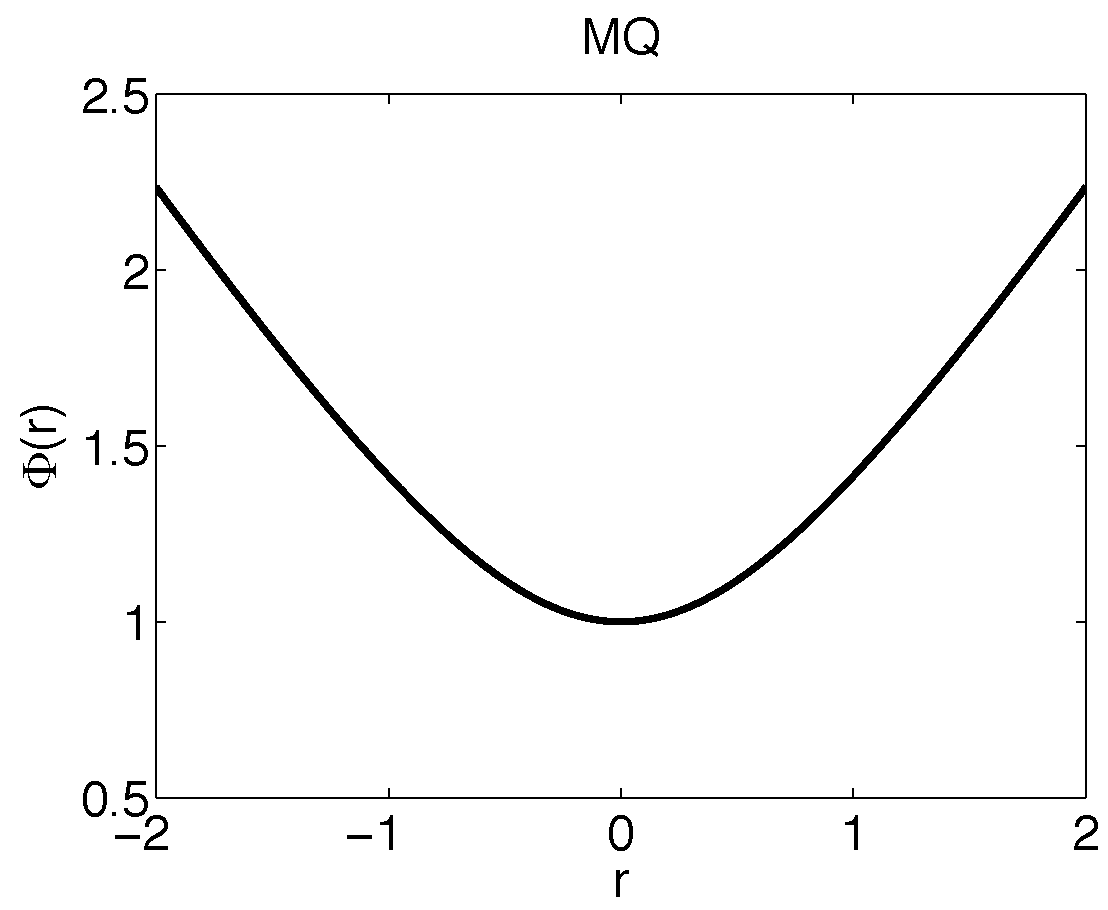
\includegraphics[width=0.25\textwidth]{matlab/mq_rbf.pdf}   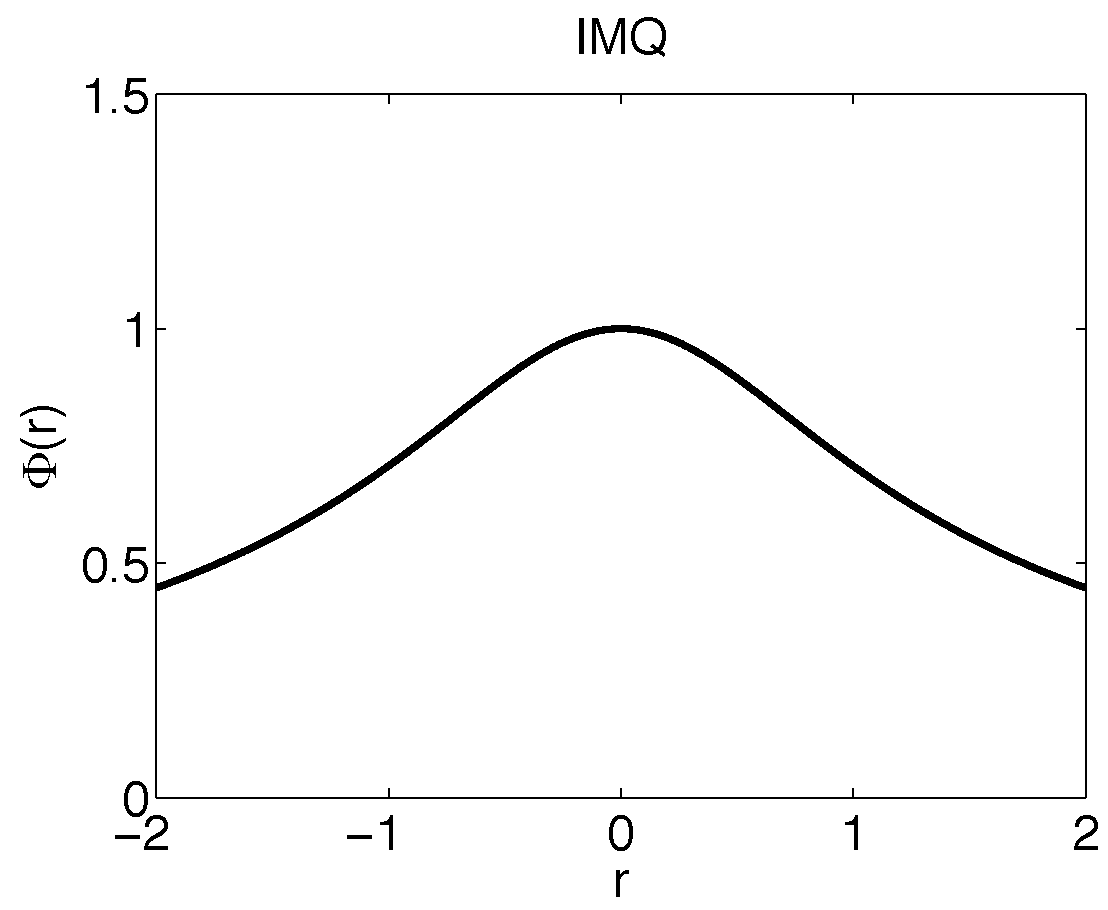
\includegraphics[width=0.25\textwidth]{matlab/imq_rbf.pdf} 
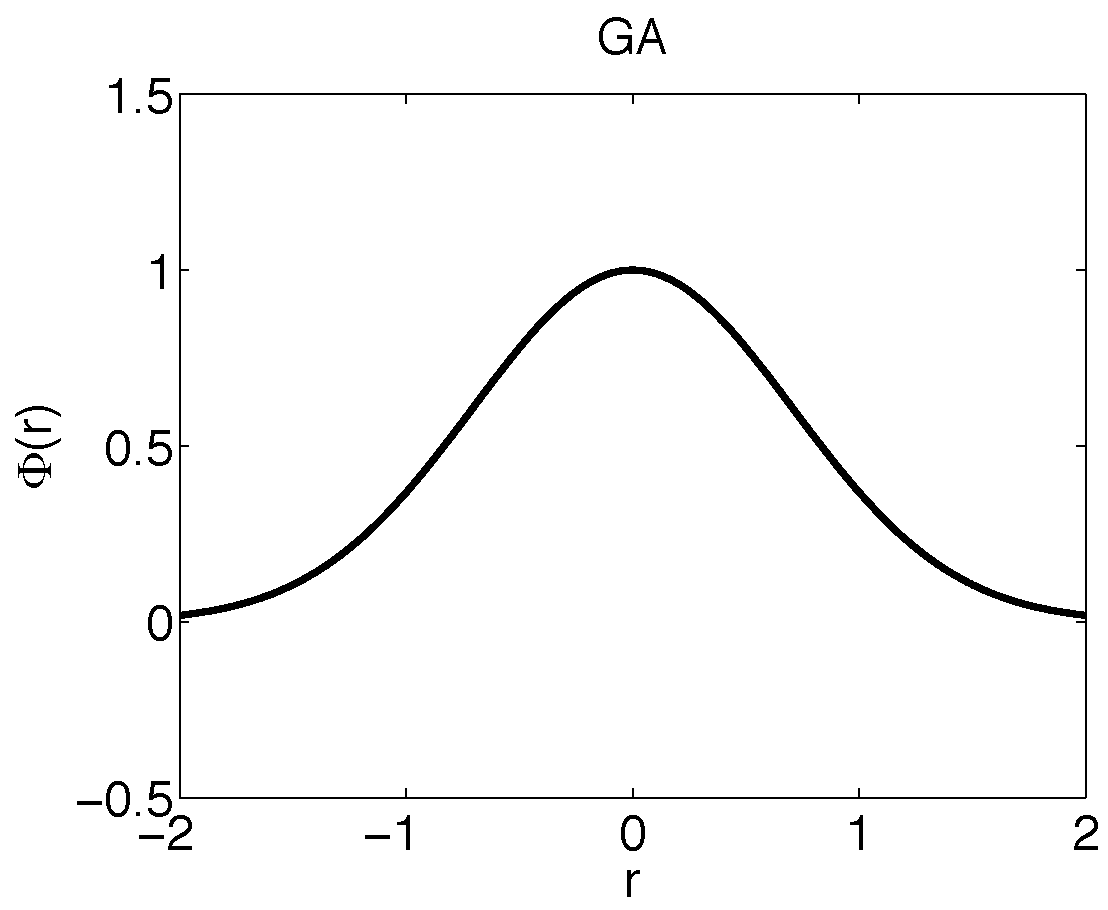
\includegraphics[width=0.25\textwidth]{matlab/ga_rbf.pdf} \\  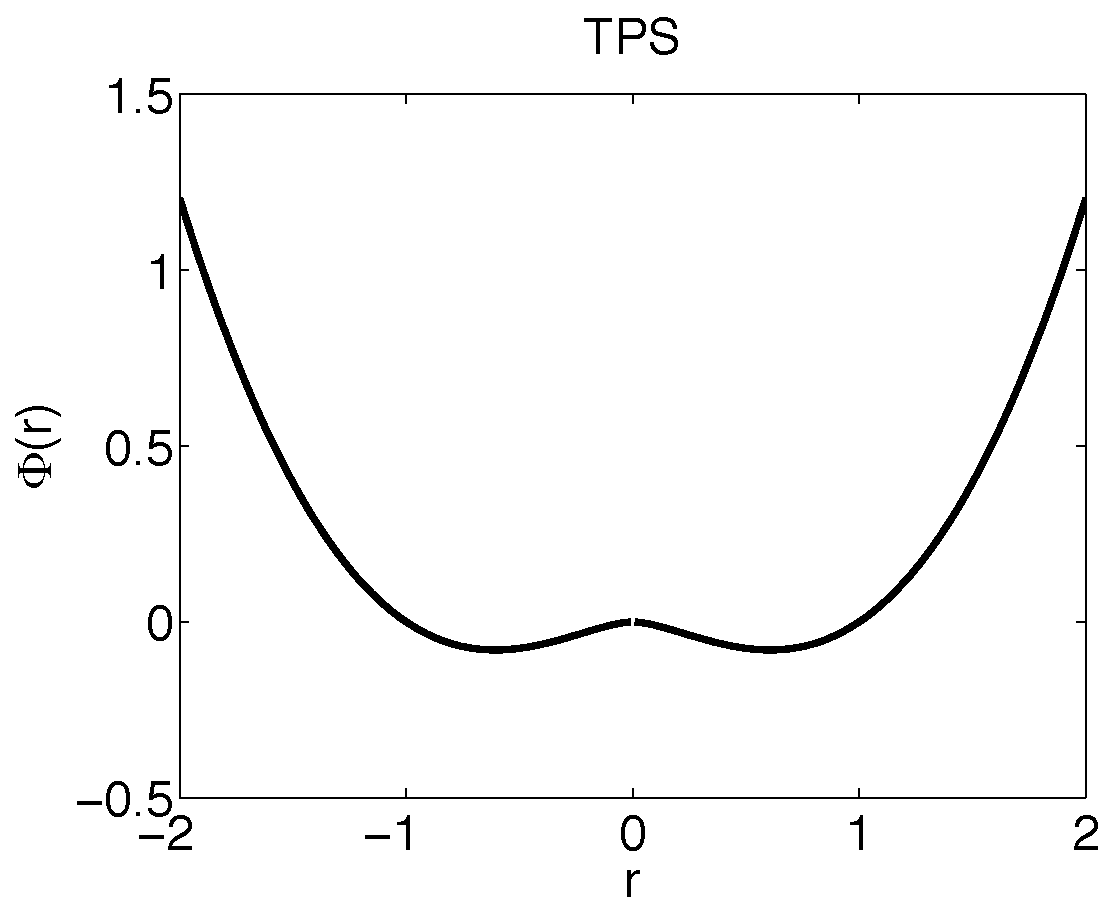
\includegraphics[width=0.25\textwidth]{matlab/tps_rbf.pdf} 
%\end{tabular} \\
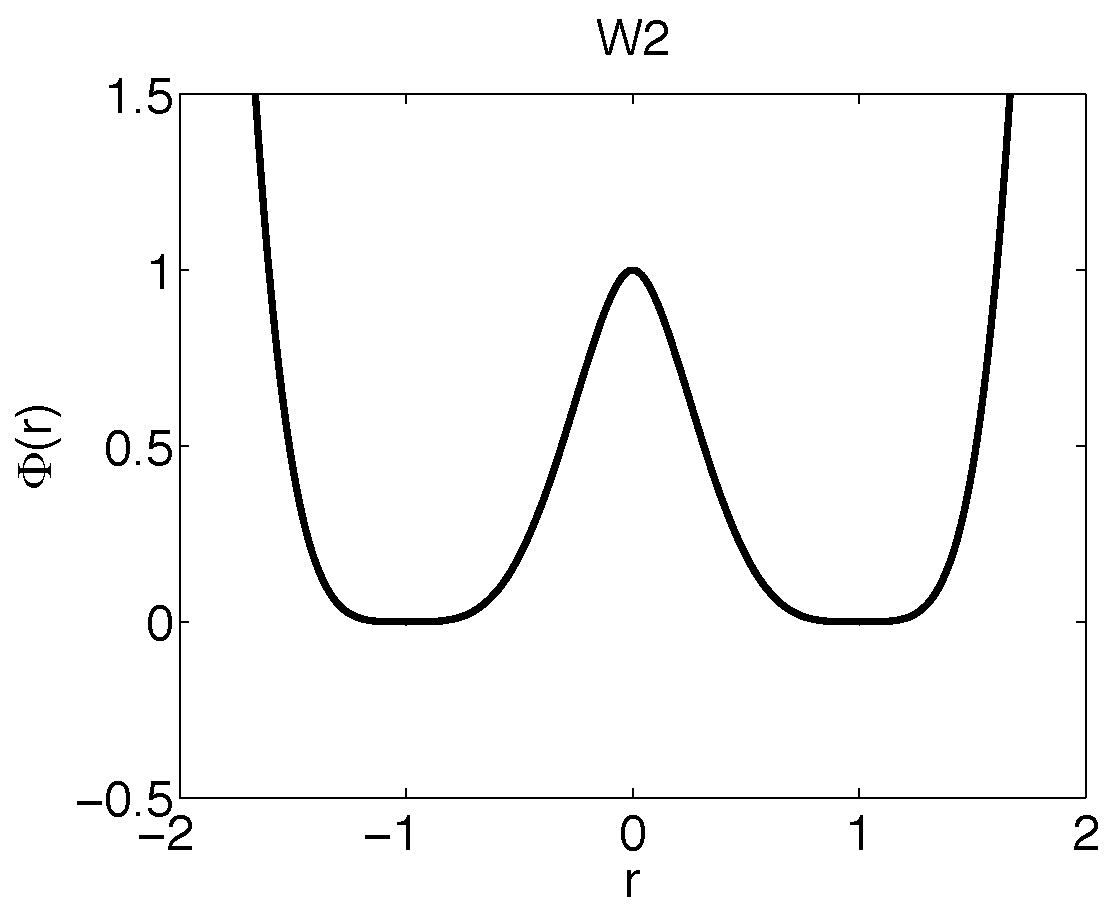
\includegraphics[width=0.25\textwidth]{matlab/w2_rbf.pdf}
\caption{Example RBF shapes from Table~\ref{tbl:rbfs} with parameter $\varepsilon=1$.}
\label{fig:rbf_examples}
\end{figure} 


\begin{figure}[t]
\centering
\begin{tabular}{cc}
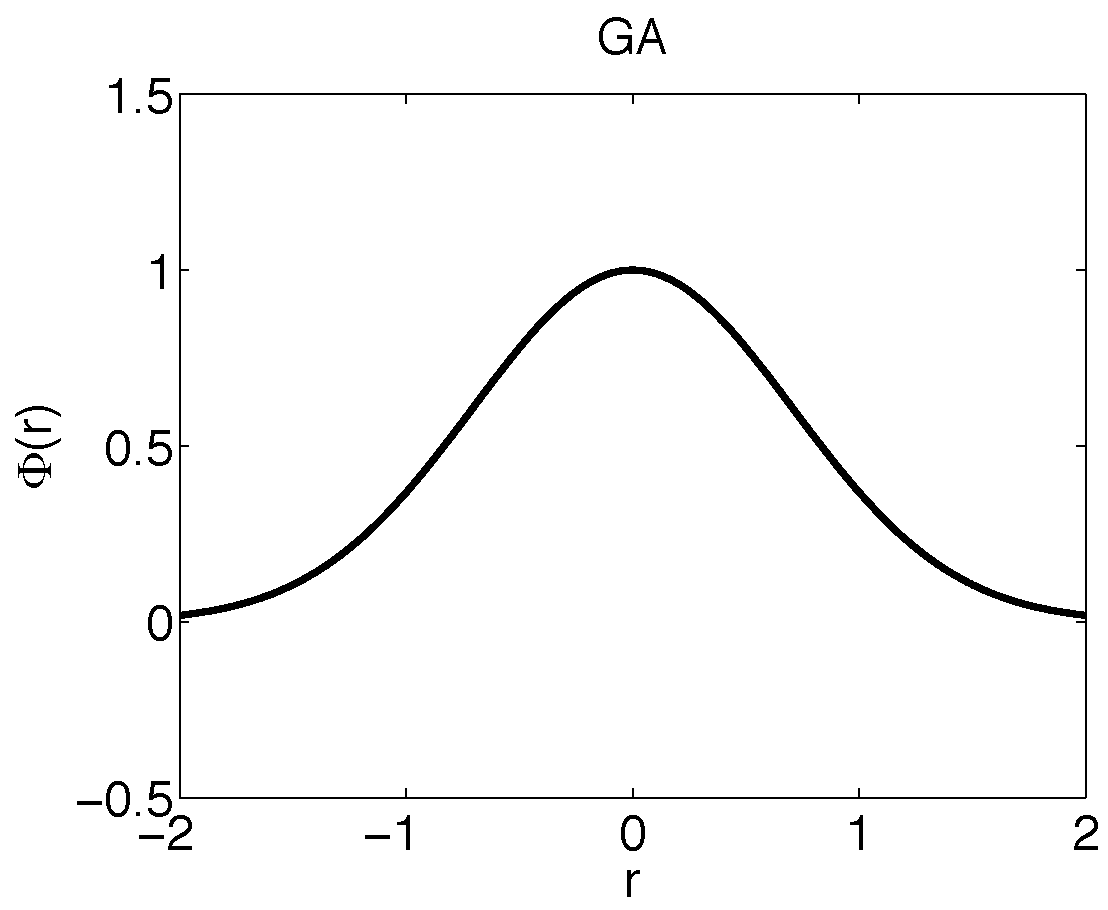
\includegraphics[width=0.25\textwidth]{matlab/ga_rbf.pdf}
\includegraphics[width=0.35\textwidth]{matlab/ga_rbf2D.eps}
\includegraphics[width=0.35\textwidth]{matlab/ga_rbf3D.eps}
\end{tabular} 
\caption{The Gaussian (GA) RBF (Table~\ref{tbl:rbfs}) with parameter $\varepsilon=1$ in dimensions 1, 2 and 3.}
\label{fig:rbf_dimension_example}
\end{figure} 

\begin{figure}[t]
    \centering
    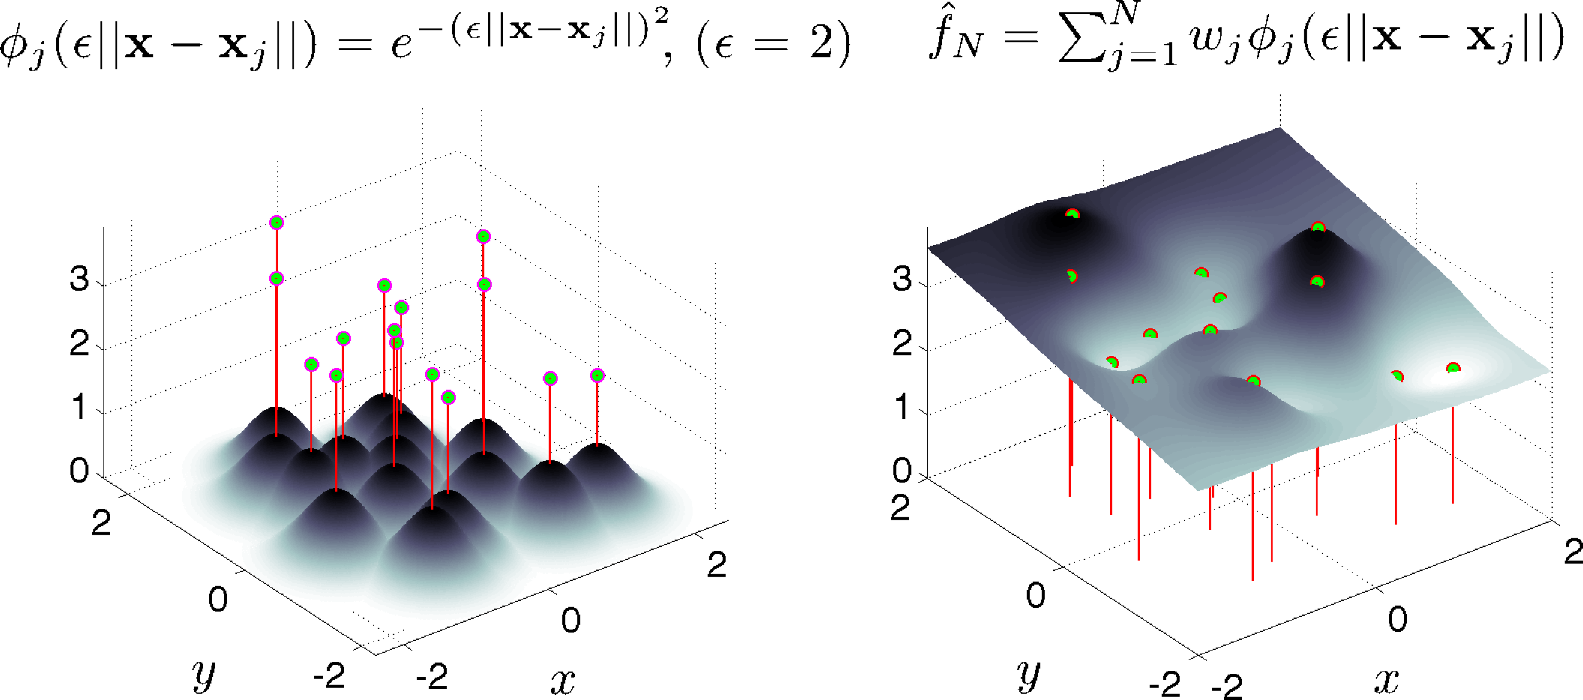
\includegraphics[scale=0.4]{figures/trimmed_interpolate2D_ga__m.pdf}
    \caption{RBF interpolation using 15 translates of the Gaussian RBF with $\epsilon=2$. One RBF is centered at each node in the domain. Linear
    combinations of these produce an interpolant over the domain passing through known function values. }
    \label{fig:rbfInterpolation}
\end{figure}

%TODO: expand with new literature since 2009
%TODO: any new methods?


RBF methods for interpolation first appeared in 1971 with Hardy's seminal research on multiquadrics
\cite{Hardy1971}. In his 1982 survey of scattered data interpolation methods \cite{Franke1982}, Franke rated multiquadrics first-in-class against 28 other methods (3 of which were RBFs) \cite{Franke1982}. Many other RBFs, 
including those presented in Table~\ref{tbl:rbfs} have been applied in literature, but for PDEs in particular, few can rival the 
attention received by multiquadrics. Recently, however, Gaussian RBFs are on the rise due to recent advances in eigenvalue stabilization and new methods for investigating the $\epsilon \rightarrow 0$ regime (see e.g., \cite{FornbergLehto11,Fornberg2011a}). 


By 1990, the understanding of the scientific community regarding RBFs was sufficiently developed for collocating PDEs \cite{Kansa1990a,Kansa1990b}. PDE collocation seeks a solution of the form
\begin{eqnarray*}
(\diffop{u})(x_i) = \sum_{j=1}^{N} \phi_j(x_i) c_j = f(x_i)
\end{eqnarray*}
where $\diffop{}$ is, in general, a nonlinear differential operator acting on $u(x)$. The solution $u(x)$ is expressed as a linear combination of $N$ basis functions $\phi_j(x)$, not necessarily RBFs: 
$$
u(x) = \sum_{i=1}^N \phi_j(x) c_j 
$$
As in the problem of RBF scattered data interpolation, $ \vc = \{c_j\} $ is the unknown coefficient vector. 
Under the assumption that $\mathcal{L}$ is a linear operator, one can collocate the differential equation. Alternatively, individual derivative operators can be expressed as linear combinations of the unknowns $u_j$ (leading to the RBF-FD methods). 
In all cases, a linear system of equations arises, with different degrees of sparsity, dependent on the chosen basis functions and how the various constraints are enforced.  While we restrict the $\phi_j(x)$ to RBFs or various operators applied to the RBFs, we note that spectral methods, finite-element or spectral-element methods can be formulated in a similar way with different choices of basis functions.  Of course, $u$ can be a vector of unknown variables ($\vc$ then becomes a matrix). 

Table~\ref{tbl:rbfcolloctypes} classifies references according to their choice of collocation method and RBF 
interpolation type. 
There are three main categories of RBF interpolation listed in Table~\ref{tbl:interp_types}. The first is \emph{Global} in the case that a single, large ($N\times N$) and 
dense matrix corresponding to globally supported RBFs is inverted; second, \emph{Compact} if compactly supported RBFs are used to 
produce a single, large, but \emph{sparse} matrix; and third, \emph{Local} if compactly supported RBFs are used to produce many small but 
dense matrices with one corresponding to each collocation point. In all three cases the matrices are symmetric and with the correct choice of RBF they are at least conditionally positive definite. The final row of Table~\ref{tbl:rbfcolloctypes} considers literature on the RBF-FD method and is discussed in depth in Chapter~\ref{chap:rbffd_method}.

\begin{table}[t]
   \centering
   \begin{tabular}{E | C | C | C | c | } % Column formatting, @{} suppresses leading/trailing space
   Interpolation Type & Dense/Sparse $A$ & Dim($A$) ($N_S \ll N$) &  \# of $A^{-1}$  & RBF Support \\ 
   \hline \hline
   Global & Dense & $N \times N$ & 1 & Global \\
   Compact & Sparse & $N \times N$ & 1 & Compact \\
   Local & Dense & $N_S \times N_S$ & N & Global/Compact
   \end{tabular}
   \caption{RBF interpolation types and properties, assuming a problem with $N$ nodes.}
   \label{tbl:interp_types}
\end{table}


We note that three types of collocation occur throughout the RBF literature: 
Kansa's unsymmetric collocation method \cite{Kansa1990a, Kansa1990b}, Fasshauer's symmetric collocation method \cite
{Fasshauer1997}, and the Direct collocation method \cite{Fedoseyev2002}. 
%TODO: classify RBF-PS applications

% While not a collocation method, RBF-FD represents the latest trend in solving PDEs with RBFs.  %A full explanation of RBF based collocation is deferred to Chapter~\ref{chap:rbf_pde}. 

We now turn to discussion of the benefits and shortcomings of each RBF method, before covering derivation of the methods. 
%Prior to launching into derivation each RBF collocation method, we first survey the classifications to highlight benefits, shortcomings, and to provide a brief historical context. A survey of related work in the RBF community that involves parallelization and optimization is deferred to Chapter~\ref{chap:parallel_rbf}. 

\subsection{Global RBF Methods}

\emph{Kansa's method} \cite{Kansa1990a, Kansa1990b} (a.k.a. unsymmetric collocation) was the first RBF method for PDEs, and is still the most frequently used method. The idea behind Kansa's method is that an 
approximate solution to the PDE can be found by finding an interpolant which satisfies the differential operator with zero residual at a set of \emph{collocation points} (these coincide with the RBF centers). To find the interpolant, the differential equation is formulated as a two block (unsymmetric) linear system with: 1) the approximation of values 
at boundary 
points with boundary data only, and 2) the approximation of interior points by directly applying the differential operator. It was 
shown in \cite{Fasshauer1997, Hon2001} that the unsymmetric linear system produced by Kansa's method does not guarantee 
non-singularity; although it is also noted that in practice singularities are rare encounters \cite{Larsson2003}. 

The second alternative for RBF collocation, is based on Hermite scattered 
data interpolation (see \cite{Wu1992}). The so-called \emph{Fasshauer} or \emph{Symmetric Collocation} method (\cite{Fasshauer1997}) 
performs a change of basis for the interpolant by directly applying the differential operator to the RBFs. It then collocates using the same approach as Kansa's method \cite{Stevens2009b, Larsson2003}. The resulting block structure of the linear system is symmetric and 
guaranteed to be non-singular \cite{Fasshauer1997}. In comparison to Kansa's method, the disadvantages of Fasshauer's method 
include: a) requirement of higher order differentiability of the basis functions (to satisfy double application of the differential operator)
% it has stronger regularity assumptions (it is Hermite interpolation), 
and b) the linear system is larger and more complex to form
%, and c) it is not ideally suited for non-linear problems
 \cite{Fasshauer2007}. As \cite{Hon2001} points out, 
the possible existence of a singularity in Kansa's method is not enough to justify the added difficulties of using Fasshauer's 
method.

%TODO: refs that refer to global RBF methods and RBF-PS as just RBF methods. 

The last collocation method, \emph{Direct Collocation}, was introduced by Fedoseyev, Friedman and Kansa
 \cite{Fedoseyev2002} and satisfies the differential operator on the interior and the boundary. Larsson and Fornberg \cite{Larsson2003} observe that this third method has a matrix structure similar to that found in Kansa's method; however, it is noted that the dimensions of the matrix blocks for each method differ. This is due to collocation constraints added for 
the differential operator applied to the boundary. Aside from the survey on RBF collocation presented by Larsson and Fornberg \cite{Larsson2003}, no related 
work was found that applied, or investigated, this method further.  

Both Kansa's method and Fasshauer's methods were shown in \cite{Fasshauer2006} to fit well in the generalized framework of pseudo-spectral methods with a subtle change in algorithm. While collocation methods explicitly compute the coefficients for a continuous derivative approximation, their alternates, referred to in literature as RBF-pseudospectral (RBF-PS) methods, never explicitly compute the interpolant coefficients. Instead, a differentiation matrix (DM) is assembled and used to approximate derivates at the collocation points only \cite{FasshauerZhang2007}. Since most computational models are simply concerned with the solution at collocation points, the change to assemble DMs as in RBF-PS is organic. 


Following the evolution of the RBF-PS algorithm, applications of global RBFs in the classic collocation sense (i.e., without the RBF-PS DMs) become impractical. This statement stems from the algorithmic complexity of each method. 
%As discussed in \cite{Fasshauer2007, FlyerWright09}, RBF methods result in matrices that are full. The 
Global RBF methods result in full matrices \cite{Fasshauer2007}. The global collocation methods then scale on the order of $O(N^3)$ floating point operations (FLOPs) to solve for weighting coefficients on a given node layout, plus $O(N^2)$ to apply the weights for derivatives. If time-stepping is required, global collocation methods must recompute the time-dependent coefficients with additional cost dominated by $O(N^3)$ operations. RBF-PS methods have similar requirements for $O(N^3)$ operations to assemble the differentiation matrix and $O(N^2)$ to apply for derivatives. However, by avoiding time-dependent coefficients, the differentiation matrix application at each time-step is only $O(N^2)$ operations. As an aside, the $O(N^3)$ complexity for each method---typically due to an LU-decomposition, with subsequent forward- and back-solves---could be reduced. While not in mainstream use by the RBF community, \cite{Morse2005} correctly points out that iterative solvers could be employed for $O(N^2)$ complexity. 
%For mid- to large-scale problems, in the unlikely event that conditioning of the system is not a limiting factor, the cost of the method is still seen as prohibitively high. 

Hon et al. \cite{Hon1999} employed Kansa's method to solve shallow water equations for Typhoon simulation.
In \cite{FlyerWright09}, Flyer and Wright employed RBF-PS (Kansa method) for the solution of shallow water equations on a sphere. Their 
results show that RBFs allow for longer time steps with spectral accuracy. The survey \cite{FlyerFornberg11} by Flyer and Fornberg showcases RBF-PS (Kansa's method) out-performing some of the of the best available methods in geosciences, namely: Finite Volume, Spectral Elements, Double Fourier, and Spherical Harmonics. When applied to problems such as transport on the sphere \cite{FlyerWright07}, shallow water equations \cite{FlyerWright09}, and 3D mantle convection \cite{WrightFlyerYuen10}, RBF-PS consistently required fewer time steps, and a fraction of the nodes for similar accuracy \cite{FlyerFornberg11}. 
%TODO: add \cite{Neves2009}

%
%In the survey on RBF collocation presented by Larsson and Fornberg \cite{Larsson2003}, it was found that performance of the 
%collocation methods depends on the choice of RBFs (i.e., whether they are infinitely smooth or piecewise smooth). Their end 
%conclusion, however, was that infinitely smooth RBFs are preferred for Elliptic PDEs as they do not require node placement 
%optimization.

%Kansa collocation
\newcommand{\kansaglobalrbf}[0]{\cite{Kansa:1990a, Kansa:1990b, Fasshauer:2006, Fornberg:2004, Mouat:2002, Hon:2001, Franke:1982, Flyer:2009b, Flyer:2007, Hon:1999, Fornberg:2008, Larsson:2003}}
\newcommand{\kansacsrbf}[0]{\cite{Fornberg:2008, Wang:2002}}
\newcommand{\kansalocalrbf}[0]{\cite{Divo:2007, Kosec:2008, Sarler:2006, Vertnik:2006}}

% Fasshauer collocation
\newcommand{\fassglobalrbf}[0]{\cite{Fasshauer:2006, Fasshauer:1997, Larsson:2003}}
\newcommand{\fasscsrbf}[0]{\cite{Liu:2005}}
\newcommand{\fasslocalrbf}[0]{\cite{Stevens:2008a, Stevens:2009a, Stevens:2009b}}

% Direct collocation
\newcommand{\directglobalrbf}[0]{\cite{Fedoseyev:2002, Larsson:2003}}
\newcommand{\directcsrbf}[0]{}
\newcommand{\directlocalrbf}[0]{}


% RBF-FD
\newcommand{\rbffdglobalrbf}[0]{N/A}
\newcommand{\rbffdcsrbf}[0]{N/A}
\newcommand{\rbffdlocalrbf}[0]{\cite{Wright:2006,Wright:2003, Shu:2003, Cecil:2004, Wright:2004, Shu:2006, Chandhini:2007}}


%\begin{sidewaystable}
\begin{table}[t]
\begin{center}
	\begin{tabular}{@{} R|C|C|C|}
		& \multicolumn{3}{c|}{RBF Interpolation Type} \\
		\hline
		Method & Global (Dense) & Compact (Sparse Global) & Local \\
		\hline \hline
		Kansa's Method &\kansaglobalrbf & \kansacsrbf & \kansalocalrbf \\
		\hdashline
		Fasshauer's Method &\fassglobalrbf & \fasscsrbf & \fasslocalrbf \\
		\hdashline
		Direct Collocation &\directglobalrbf & \directcsrbf & \directlocalrbf \\
		\hdashline
		RBF-FD & \rbffdglobalrbf & \rbffdcsrbf & \rbffdlocalrbf \\
		\hline
	\end{tabular}
\end{center}
\caption{Classification of references based on choice of RBF interpolation types and method for solving PDEs. References may appear in multiple cells according to the breadth of their research.}
\label{tbl:rbfcolloctypes}
\end{table}
%\end{sidewaystable}




\subsection{Compactly Support RBFs} 

Thus far, all cases of collocation and interpolation mentioned have assumed globally supported RBFs. While global RBFs are well-studied and have nice properties, a major limitation is the large, dense system that must be solved. One alternative to global support is to use a set of compactly supported RBFs (CSRBFs) that are defined as: 
\begin{equation}
\phi(r) = \begin{cases} \varphi(r) & r \in [0,1]\\
0 & r > 1
\end{cases}
\label{eqn:csrbf}
\end{equation}
where a cut-off radius is defined past which the RBF (in this case $\varphi(r)$) has no influence on the interpolant. Note that the radius can be scaled to fit a desired support. Methods that leverage CSRBFs produce a global interpolation matrix that is \emph{sparse} and therefore results in a system that is more efficiently assembled and solved with smaller memory requirements \cite{Fasshauer2007}. The actual complexity estimate of the CSRBF method depends on the sparsity of the problem as well as the ordering of the assembled system. Assuming $n \ll N$ where $n$ represents the number of nodes in support, \cite{Zhang2004} lists the complexity as dominated by $O(N)$ for properly structured systems within MATLAB, and the investigation in \cite{Morse2005} found $O(N^{1.5})$ consistent with the estimate provided by their choice of general sparse solver package. A multi-level CSRBF method, introduced by Fasshauer \cite{Fasshauer2007}, collocates solutions over multiple grid refinements to achieve reduced $O(N)$ complexity, but the method is plagued by poor convergence. It is also worth noting that in the context of CSRBFs, analogues to Kansa's method and Fasshauer's method are known by the names \emph{radial point interpolation method (RPIM)} \cite{Wang2002} and \emph{radial point interpolation collocation method (RPICM)} \cite{Liu2005}, respectively. A more thorough survey of CSRBF history can be found in \cite{Fasshauer2007,Iske2004}.

CSRBFs have attracted a lot of attention in applications. For example, in the field of dynamic surface and image deformation, compact support allows for local transformations which do not induce global deformation (see e.g., \cite{Yang2008, Lin2009, Correa2007}). 




\subsection{Local RBF Methods}
% TODO: review these papers
Around 2005, \v{S}arler and Vertnik \cite{Sarler2006, Vertnik2006} demonstrated that if compactly supported RBFs are chosen, the traditional global 
collocation matrix from Kansa's method, can be avoided altogether in favor of small localized collocation matrices defined for 
each node. Local collocation still faces possible ill-conditioning and singularities 
like global collocation, but make it easier to distribute computation across parallel systems. Also, the smaller linear systems can be 
solved 
with less conditioning issues. In \cite{Sarler2006}, the authors consider 2D diffusion problems. Divo and Kassab \cite{Divo2007} 
employ the 
method for Poisson-like PDEs including fluid flow and heat transfer. Kosec and \v{S}arler \cite{Kosec2008} apply the 
same technique to solve coupled heat transfer and fluid flow problems.

In similar fashion, Stevens et al. \cite{Stevens2009a} introduced a local version of 
Fasshauer's method called \emph{local Hermitian interpolation}. The authors have applied their method to 3D soil 
problems based on transient Richards' equations \cite{Stevens2008a, Stevens2009a, Stevens2009b}.



\section{Comparison of RBF Methods}

We now detail RBF methods for PDEs leading up to the derivation of RBF-FD. 

Following \cite{Mouat2002}, consider a PDE expressed in terms of a (linear) differential operator, $\diffop$: 
\begin{eqnarray*}
\diffop{u} & = & f \on{\Interior} \\
u &=& g \on{\Boundary}
\end{eqnarray*}
where $\Interior$ is the interior of the physical domain, $\Boundary$ is the boundary of $\Interior$ and $f,g$ are known explicitly. In the case of a non-linear differential operator, a Newton's iteration, or some other method, can be used to linearize the problem (see e.g., \cite{WrightFornberg06}); of course, this increases the complexity of a single time step. Then, the unknown solution, $u$, which produces the observations on the right hand side can be approximated by an interpolant function $u_{\phi}$ expressed as a linear combination of radial basis functions, $\{\phi_j(x) = \phi(\vectornorm{x-x_j})\}_{j=1}^{N}$, and polynomial functions$\{P_l(x)\}_{l=1}^{M}$:
\begin{equation}
	u_{\phi}(x) = \sum_{j=1}^{N}  \phi_j(x) c_{j} + \sum_{l=1}^{M}  P_l(x) d_{l}, \hskip1.5em P_l(x) \in \Pi^{d}_{p}
	\label{eqn:pde_approx}
\end{equation}
where $\phi_j(x) = \vectornorm{x - x_j}_2$ (Euclidean distance). The 
second sum represents a linear combination of polynomials that enforces zero approximation error
 when $u(x)$ is a polynomial of degree less than or equal to $p$. The variable $d$ is the 
 problem dimension (i.e., $u_{\phi}(x) \in \R^{d}$). 
%\toevan{Finish to end of paragraph} 
To eliminate degrees of freedom for well-posedness, $p$ should be greater than or equal to the order of the chosen RBF
 (see Table~\ref{tbl:rbfs}) \cite{Iske2004}.  
Note that Equation~\ref{eqn:pde_approx} is evaluated 
 at $\{x_j\}_{j=1}^{N}$ 
data points through which the interpolant is required to pass with zero residual.  We refer to 
the $x_j$'s as \emph{collocation points} (a.k.a. trial points), taken as the RBF centers. The test points, $x$, usually coincide with collocation points, although this is not a requirement. 
%$P_l(x)$ is needed to eliminate degrees of freedom for well-posedness \cite{Iske:2004}. 

To clarify the role of the polynomial part in Equation~\ref{eqn:pde_approx}, it is necessary to
put aside the PDE for the moment and consider only the problem of \emph{scattered data 
interpolation} with Radial Basis Functions.

\subsection{RBF Scattered Data Interpolation}
 Borrowing notation from \cite{Fasshauer2007, Iske2004}, 
we seek an interpolant of the form
\begin{eqnarray*}
f(x) = \sum_{j=1}^{N} \phi_j(x) c_{j}  \label{eq:rbf_scattered_data_interp}
\end{eqnarray*}
where $f(x)$ is expressed as a scalar product between the unknown coefficient weights $c_j$ and the radial basis functions $\phi_j(x)$.

To obtain the unknown coefficients, $c_j$, form a linear system in terms of the $N$ RBF centers:
\begin{eqnarray*}
f(x) & = & \sum_{j=1}^{N} c_{j}  \phi_j(x)  \hskip1.5em \textrm{for\ } x = \{x_j\}_{j = 1}^{N} \\
 \parray{c}{ f } & =&  \barray{c}{\phi}\parray{c}{ c } 
\end{eqnarray*}
The invertibility of this system depends on the choice of RBF, so one typically chooses a function that is positive definite to avoid issues. It has been shown (see \cite{Fasshauer2007, Iske2004}) that some choices of RBFs (e.g. multiquadrics and thin-plate splines \cite{Hon2001}) are not positive definite and therefore there is no guarantee that the approximation is well-posed. A sufficient condition for well-posedness is that the matrix be \emph{conditionally positive definite}. In \cite{Fasshauer2007}, Fasshauer demonstrates that conditional positive definiteness is guaranteed when Equation~\ref{eqn:pde_approx} exactly reproduces functions of degree less than or equal $m$. 
For RBF scattered data interpolation in one dimension, this can be achieved by adding a polynomial of order $m$ with $M =$${m+1}\choose{1}$ terms (e.g., $x^0, x^1, \cdots, x^{m}$). 
%For $\R^2$, the terms would be: $1, x, y, xy, x^2y, xy^2, \cdots, x^{m}y^{m-1}, x^{m-1}y^{m}, x^my^m$. 
In $\R^d$, $M =$${m+d}\choose{d}$ \cite{Iske2004}, giving
\begin{eqnarray}
\sum_{j=1}^{N} c_{j}  \phi_j(x)  +  \sum_{l=1}^{M} d_{l} P_l(x) & = & f(x),  \hskip1.5em  P_l(x) \in \Pi^{d}_{m} \label{eqn:interpolation_constraints} \\
\left[ \begin{array}{c c} 
	\phi & P
	\end{array} \right] \left( \begin{array}{c}
							c \\
							d
							 \end{array}
						 \right) & = & \parray{c}{ f } \nonumber
\end{eqnarray}
where the second summation (referred to as \emph{interpolation conditions} \cite{Iske2004}) ensures the minimum degree of the interpolant. Refer to Table~\ref{tbl:rbfs} for a short list of recommended RBFs and minimally required orders of $m$. This document prefers the Gaussian RBF. Notice, in Equation~\ref{eqn:interpolation_constraints}, that the interpolation conditions add $M$ new degrees of freedom, so we must provide $M$ 
additional constraints to square the system. In this case:
$$
\sum_{j=1}^{N} c_{j} P_l(x_j) = 0,  \hskip1.5em  l=1,..., M 
$$
or 
\begin{eqnarray}
P^T {c}  = {0}. 
\label{eqn:extra_constraints}
\end{eqnarray}
It is now possible again to write the interpolation problem as a complete linear system using Equations~\ref{eqn:interpolation_constraints} and ~\ref{eqn:extra_constraints}:%as
\begin{eqnarray}
 \underbrace{\left[ \begin{array}{c c} 
	\phi & P \\
	P^T & 0
	\end{array} \right]}_{A} \left( \begin{array}{c}
							c \\
							d
							 \end{array}
						 \right) = \left( \begin{array}{c}
							f \\
							0
							 \end{array}
						 \right) \label{eq:solve_rbf_scattered_interp}
\end{eqnarray}
%This system then produces coefficients capable of exactly approximating data from polynomials of degree less than or equal to $m$ \cite{Fasshauer2007}. 
Equation~\ref{eq:solve_rbf_scattered_interp}---typically a dense system except in the case of RBFs with compact support---can be solved efficiently via standard methods like LU-decomposition.  With the coefficients, the interpolant can be sampled at any test points, $\{x_i\}_{i=1}^{n}$, by substitution into Equation~\ref{eq:rbf_scattered_data_interp}:
\begin{eqnarray}
f(x_i) & = & \sum_{j=1}^{N} c_{j}  \phi_j(x_i) +  \sum_{l=1}^{M} d_{l} P_l(x_i)  \nonumber \\
 & = & \left. \underbrace{\left[ \begin{array}{c c} 
       \phi &  P
	\end{array} \right]}_{B} 
	  \left( \begin{array}{cc}  c \\ d  \end{array} \right) \ \right|_{x={x_i}}
	\label{eqn:interpolate_x}
\end{eqnarray}


\subsection{Reconstructing Solutions for PDEs}
In the next few subsections, we will consider collocation equations based on this general form: 
\begin{eqnarray*}
\diffop{u_\phi(x)} &=& f(x) \on{\Interior} \label{eqn:colloc_interior}\\ 
\boundop{u_\phi(x)} &=& g(x) \on{\Boundary}  \label{eqn:colloc_boundary} 
\end{eqnarray*}
where the methods presented below will apply the differential operators, $\diffop{}$ and $\boundop{}$, to different choices of $u_\phi$ and different sets of collocation points. In many applications $\diffop{}$ is chosen as a differential operator (e.g., $\pd{}{x}$, $\nabla$, $\nabla^2$) and $\boundop = I$ (i.e. identity operator for Dirichlet boundary conditions) for PDEs. For RBF scattered data interpolation, $\diffop{} = I$. There are also  applications where $\diffop{}$ is a convolution operator (see e.g., \cite{Carr2001, Carr2003}) capable of smoothing/de-noising a surface reconstructed from point clouds. 

%TODO: label x_j's as TRIAL and x_is as TEST points
%\section{Approximating the Solution}
For all the methods that follow a linear system is generated: 
$$
A_{\diffop{}}  \left( \begin{array}{cc}  c \\ d  \end{array} \right)  =  \left( \begin{array}{cc}  f \\ 0  \end{array} \right) 
$$
\begin{equation}
  \left( \begin{array}{cc}  c \\ d  \end{array} \right) = A^{-1}_{\diffop{}}  \left( \begin{array}{cc}  f \\ 0  \end{array} \right) \nonumber
  %\label{eqn:solve_coeffs}
 \end{equation}
 where matrix $A_{\diffop{}}$ depends on the choice of collocation method. 
 % TODO: fix use of A_diffop; "but contains $\diffop{\phi} = \phi_\diffop{}$. 
Once the linear system is solved, the value $u(x)$ is reconstructed at the test points following Equation~\ref{eqn:interpolate_x}:
\begin{eqnarray}
u(x) & \approx &  \left.
\left[ \begin{array}{c c} 
       \phi &  P
	\end{array} \right]
	  \left( \begin{array}{cc}  c \\ d  \end{array} \right)  \ \right|_{x={x_i}} \nonumber\\
	 & \approx & B A^{-1}_\diffop{} \left( \begin{array}{cc}  f \\ 0  \end{array} \right) 
	\label{eqn:solve_u}
\end{eqnarray}
Likewise, to obtain differential quantities we have: 
\begin{eqnarray*}
\diffop{u}(x) & \approx & \left.
\left[ \begin{array}{c c} 
       \phi_{\diffop{}} &  P_{\diffop{}}
	\end{array} \right]
	  \left( \begin{array}{cc}  c \\ d  \end{array} \right)  \ \right|_{x={x_i}} \\
  	 & \approx & B_{\diffop{}} A^{-1}_\diffop{} \left( \begin{array}{cc}  f \\ 0  \end{array} \right)
	\label{eqn:solve_uxx}
\end{eqnarray*}
%where $\phi_{\diffop}$ is the analytic RBF with 

%TODO: \subsection{Applying Methods for PDEs}
%TODO: \subsubsection{Explicit PDEs}
%TODO: \subsubsection{Implicit PDEs} 

%Here we substitute $B$ for test samples in Equation~\ref{eqn:solve_u} to get the reconstructed solution:
%\begin{eqnarray}
%u(x) = B A^{-1}_\diffop{} \left( \begin{array}{cc}  f \\ 0  \end{array} \right)
%	\label{eqn:solve_rbf}
%\end{eqnarray}
%where the vector-matrix inner product $(A A^{-1}_{\diffop{}})$ is a row-vector. Since the coefficient vectors ${c}$ and ${d}$ are the same for all $x_i$, we can group the evaluation of $\diffop{u(x_i)}$ for $i=1,...,n$ as a matrix-vector multiplication where the matrix rows correspond to $(A_\diffop{} A^{-1})$ for each $x_i$. 


%TODO: mention equation~\ref{eqn:solve_rbf} can be precomputed DM applied to f for collocation points in pseudo-spectral method.  
%Relevant to the discussion of RBF-PS and computational and memory efficient global RBF methods, if $A$ contains rows corresponding to the interpolation problem can be rewritten independent of coefficients by assembling a differentiation 
 
\subsection{PDE Methods} 

Now, since $u_{\phi}(x)$ from Equation~\ref{eqn:pde_approx} cannot (in general) satisfy the PDE everywhere, we enforce the PDE at a set of collocation points, which are  distributed over both the interior and the boundary. Again, these points do not necessarily coincide with the RBF centers, but it is convenient for this to be true in practice. Also, for each of the methods the choice of RBF can be either global, resulting in a large dense system, or compact, resulting in a large sparse system. 

\subsubsection{Kansa's Method}

The first global RBF method for PDEs, \emph{Kansa's method} \cite{Kansa1990a, Kansa1990b}, collocates the solution through known values on the boundary, while constraining the interpolant to satisfy the PDE operator on the interior. This is equivalent to choosing $u_\phi$ according to Equation~\ref{eqn:pde_approx}. The resulting system is given by \cite{Mouat2002}; assuming that $\diffop{}$ is a linear operator, 
\begin{eqnarray}
\diffop{u_\phi(x_i)} = \sum_{j=1}^{N}c_j\diffop{\phi_j(x_i)} + \sum_{l=1}^{M}d_l \diffop{P_l(x_i)} &=&f(x_i)  \hskip1.5em i = 1,...,n_I  \label{eqn:kansa_interior} \\ 
\boundop{u_\phi(x_i)} = \sum_{j=1}^{N}c_j \boundop{\phi_j(x_i)} + \sum_{l=1}^{M}d_l \boundop{P_l(x_i)} &=& g(x_i)  \hskip1.5em i = n_I + 1, \cdots, n \label{eqn:kansa_boundary} \\
\sum_{j=1}^{N} c_j P_l(x_j) & = & 0 \hskip3.0em l=1,\cdots,M \label{eqn:kansa_constraints} 
\end{eqnarray}
where $n_I$ are the number of interior collocation points, with the number of boundary collocation points equal to $n - n_I$. First, observe that the differential operators are applied directly to the RBFs inside summations, rather than first solving the scattered data interpolation problem and then applying the operator to the interpolant.  Second, since the basis functions are known analytically, it is possible (although sometimes painful) to derive $\diffop{\phi}$ (refer to \cite{Fasshauer2007} for RBF derivative tables); the same is true for the polynomials $P_l$. 

We can now reformulate Kansa's method as the linear system: 
\begin{eqnarray}
\underbrace{\left[ \begin{array}{c c} 
	\phi_\diffop{} & P_\diffop{} \\
	\phi_\boundop{} & P_\boundop{} \\
	P^T & 0
	\end{array} \right]}_{A_{\diffop{}}}  \left( \begin{array}{c}
							{c} \\
							{d}
							 \end{array}
						 \right) = \left( \begin{array}{c}
							{f} \\
							{g} \\
							0
							 \end{array}
						 \right) 
	\label{eqn:kansa_method}
\end{eqnarray}
% TODO: add underline stating that matrix is A. 


where $\phi_\diffop{} = \diffop{\phi}$, $P_\diffop{} = \diffop{P}$ are the interior components (Equation~\ref{eqn:kansa_interior}), $\phi_\boundop{}$ and $P_\boundop{}$ are the boundary components (Equation~\ref{eqn:kansa_boundary}), and $P^T = \left[P_\diffop{}^T \ \ P_\boundop{}^T\right]$ are constraints for both interior and boundary polynomial parts (Equation~\ref{eqn:kansa_constraints}). From Equation~\ref{eqn:kansa_method} it should be clear why Kansa's method is also known as the \emph{Unsymmetric} collocation method. 

%\toevan{Isn't $N+M=n$? For each case, you must put the proper relationships between $N$, $M$, $n_I$, $n$ so that the number of constraints equals the number of relations.}
Recall that the matrix in Equation~\ref{eqn:kansa_method} has no guarantee of non-singularity \cite{Fasshauer1997}; however, singularities are rare in practice \cite{Larsson2003}. 

\subsubsection{Fasshauer's Method}

\emph{Fasshauer's method} \cite{Fasshauer1997} addresses the problem of singularity in Kansa's method by assuming the interpolation to be Hermite. That is, it requires higher differentiability of the basis functions (they must be at least $C^k$-continuous if $\diffop{}$ is of order $k$). Leveraging this assumption, Fasshauer's method chooses: 
\begin{eqnarray}
u_\phi(x_i) & = & \sum_{j=1}^{N_I}  c_j \diffop{\phi_j(x_i)} + \sum_{j=N_{I} + 1}^{N} c_j \boundop{\phi_j(x_i)} + \sum_{l=1}^{M}d_l P_l(x_i)
\label{eqn:fasshauer_approx}
\end{eqnarray}
as the interpolant passing through collocation points. Note $N_I$ is used here to specify the number of RBF centers in the interior of $\Omega$. Here the interpolant is similar to Equation~\ref{eqn:pde_approx}, but a change of basis functions is used for the expansion: $\diffop{\phi_j(x)}$ on the interior and $\boundop{\phi_j(x)}$ on the boundary.

Substituting Equation~\ref{eqn:fasshauer_approx} into Equations~\ref{eqn:kansa_interior}-\ref{eqn:kansa_constraints} we get: 
\begin{eqnarray}
\sum_{j=1}^{N_I}c_j\diffop^2{\phi_j(x_i)} + \sum_{j=N_I+1}^{N}c_j\diffop{\boundop{\phi_j(x_i)}} + \sum_{l=1}^{M}d_l \diffop{P_l(x_i)} &=&f(x_i)  \hskip1.5em i = 1,...,n_I  \label{eqn:fasshauer_interior} \\ 
\sum_{j=1}^{N_I}c_j\boundop{\diffop{\phi_j(x_i)}} + \sum_{j=N_I+1}^{N}c_j\boundop^2{\phi_j(x_i)} + \sum_{l=1}^{M}d_l \boundop{P_l(x_i)} &=& g(x_i)  \hskip1.5em i = n_I + 1,..., n \label{eqn:fasshauer_boundary} \nonumber \\
\sum_{j=1}^{N_I} c_j \diffop{P_l(x_j)} + \sum_{j=N_I + 1}^{N} c_j \boundop{P_l(x_j)} &=& 0 \hskip3.0em l=1,...,M \label{eqn:fasshauer_constraints} \nonumber 
\end{eqnarray}
which becomes the following: 
\begin{eqnarray}
\underbrace{\left[ \begin{array}{c c c} 
	\phi_{\diffop{}\diffop{}} & \phi_{\diffop{}\boundop{}} & P_\diffop{} \\
	\phi_{\boundop{}\diffop{}} & \phi_{\boundop{}\boundop{}} & P_\boundop{} \\
	P^T_{\diffop{}} & P^T_{\boundop{}} & 0 \\
	\end{array} \right]}_{A_{\diffop{}}} \left( \begin{array}{c}
							{c} \\
							{d}
							 \end{array}
						 \right) = \left( \begin{array}{c}
							{f} \\
							{g} \\
							0
							 \end{array}
						 \right) 
	\label{eqn:fasshauer_method}
\end{eqnarray}
Note that $\phi_{\diffop{}\diffop{}}$ represents the first summation in Equation~\ref{eqn:fasshauer_interior}. 
%The linear system generated by Fasshauer's method reveals an interesting structure: namely, the subscripts $\diffop{}$ and $\boundop{}$ show blocks of influence in the matrix. For example, the interior RBF centers influence collocation on the interior collocation points ($\phi_{\diffop{}\diffop{}}$), boundary centers influence collocation on the interior ($\phi_{\diffop{}\boundop{}}$), interior centers influence collocation on the boundary($\phi_{\boundop{}\diffop{}}$), and so forth. In the case where the collocation points and RBF centers do not coincide, the subscripts would also indicate which set of points the operators are applied to \cite{Stevens2009b}. 

The symmetry of Fasshauer's (\emph{symmetric collocation}) method is apparent in Equation~\ref{eqn:fasshauer_method}. Likewise, it is clear that the symmetric method requires more storage and computation to solve compared to Kansa's method. However, based on the assumption that collocation points coincide with RBF centers, the symmetry reduces storage requirements by half. 
 
%\toevan{Its important to understand that Fasshauer's method reveals a general structure of collocation methods. Specifically, using the general notation in Equation~\ref{eqn:fasshauer_method}, we could separate the operators intended for RBF centers from those intended for the collocation points, which would allow reproduction of the cases: kansa, fasshauer, direct. Where kansa chooses $\diffop_{centers} = 1$,  $\diffop_{colloc} = \diffop$, and $\boundop_{both} = 1$. Fasshauer chooses  $\diffop_{centers} = \diffop{}$, $\diffop_{colloc} = \diffop$ and  $\boundop_{both}=1$. Direct chooses  $\diffop_{centers} = 1$ $\diffop_{colloc} = \diffop$, $\boundop_{centers}=1$, $\boundop_{colloc} = \diffop{}$. Thus Direct is a hybrid of Kansa and Fasshauer. Also, there are additional cases visible here which have not been considered in literature.} 
 
\subsubsection{Direct Collocation}

In \emph{Direct collocation} (see \cite{Larsson2003, Fedoseyev2002}, the interpolant is chosen as Equation~\ref{eqn:pde_approx} (the same as Kansa's method). However, the Direct method collocates both the interior and boundary operators at the boundary points:
%\toevan{Add boundary term and specify that Kansa's method is a special case that sets boundary to 0 (i.e. Dirichlet)}  
\begin{eqnarray}
\sum_{j=1}^{N}c_j\diffop{\phi_j(x_i)} + \sum_{l=1}^{M}d_l \diffop{P_l(x_i)} &=&f(x_i)  \hskip1.5em i = 1,...,n  \label{eqn:direct_interior} \\ 
\sum_{j=1}^{N}c_j\boundop{\phi_j(x_i)} + \sum_{l=1}^{M}d_l \boundop{P_l(x_i)} &=& g(x_i)  \hskip1.5em i = 1,..., n_B=n-n_I \label{eqn:direct_boundary} \nonumber \\
 \sum_{j=1}^{N} c_j P_l(x_j) &=& 0 \hskip3.0em l=1,...,M \label{eqn:direct_constraints} \nonumber 
\end{eqnarray}
Reformulating as a linear system we get: 
\begin{eqnarray}
\left[ \begin{array}{c c} 
	\phi_{\diffop{}} & P_\diffop{} \\
	\phi_{\boundop{}} & P_\boundop{} \\
	P^T  & 0 \\
	\end{array} \right] \left( \begin{array}{c}
							{c} \\
							{d}
							 \end{array}
						 \right) = \left( \begin{array}{c}
							{f} \\
							{g} \\
							0
							 \end{array}
						 \right) 
	\label{eqn:direct_method}
\end{eqnarray}

While the final system in Equation~\ref{eqn:direct_method} is structured the same as Kansa's method (Equation~\ref{eqn:kansa_method}), %and is often confused with it (see e.g. \cite{Fasshauer2007}), 
careful inspection of the index $i$ in Equations~\ref{eqn:kansa_interior} and \ref{eqn:direct_interior} reveals that Direct collocation produces a larger system. %Similar to Fasshauer's method, the larger system is due to additional information about influence of centers on collocation points (e.g.,  boundary on interior, interior on boundary, interior on interior, etc.). Unlike Fasshauer's method, the Direct collocation approach does not change the basis functions in the interpolant making it less obvious to readers when when a linear system represents Kansa's method or the Direct method. 


%DONE: RBF-PS
\subsubsection{RBF-PS}
%DONE: shown to solve great things
%DONE: in most cases nodes are constant

The extension of global collocation to traditional pseudo-spectral form was introduced by Fasshauer in \cite{Fasshauer2006}. Dubbed RBF-PS, the method utilizes the same logic from Kansa's and Fasshauer's collocation methods to form matrix $A_{\diffop{}}$ (i.e., $A_\diffop{}$ can be either Equation~\ref{eqn:kansa_method} or \ref{eqn:fasshauer_method}). However, RBF-PS subtly assumes the solution, $u(x)$, is only required at collocation points (i.e., $\{x_i\} = \{x_c\}$) \cite{Fasshauer2006, Fasshauer2007}. Then, extending Equation~\ref{eqn:solve_u}, RBF-PS gives:
\begin{eqnarray}
u(x) & = & \left( B A^{-1}_\diffop{} \right) \left( \begin{array}{cc}  f \\ 0  \end{array} \right) \nonumber \\
& = & D^T_{\diffop{}} \left( \begin{array}{cc}  f \\ 0  \end{array} \right) \label{eq:rbf-ps}.
\end{eqnarray}
where $D_\diffop{}$ is a discrete differentiation matrix (DM) for the operator $\diffop{}$.
Here, $D_\diffop{}$ is independent of the function $f(x)$ and is assembled by solving the system: 
\begin{eqnarray}
D_{\diffop{}} & = & A^{-T}_{\diffop{}} B^T
\end{eqnarray}
An LU-decomposition ($O(N^3)$) in preprocessing with forward- and back-solves ($O(N^2)$) are fitting to efficiently solve the multiple RHS system\cite{WrightFlyerYuen10,Fasshauer2007}. 

Since matrix $D_{\diffop{}}$ is independent of functions $u(x)$ and $f(x)$, the matrix requires update only if the RBF centers move---a compelling benefit for time-dependent problems on stationary nodes. The complexity of RBF-PS for time-dependent solutions is then reduced to a matrix-vector multiply ($O(N^2)$) for each time-step. In contrast, classic RBF collocation methods also construct LU factors of $A_{\diffop{}}^{-1}$ in preprocessing, but delay application of forward- and back-solves to acquire time-dependent weighting coefficients at each time-step. This is then followed by the pre-multiply of $B$ (i.e., additional $O(N^2)$) to complete the time-step.
 


%TODO: RBF-PS literature \cite{Fasshauer2006, Fasshauer2007}\cite{FasshauerZhang2007}\cite{WrightFlyerYuen10}


\subsection{Local Methods}

Another trend in RBF methods is to use compact support to produce local linear systems defined at each collocation point. Examples of this include \cite{Sarler2006, Vertnik2006} for Kansa's method, \cite{Stevens2008a, Stevens2009a, Stevens2009b} for Fasshauer's method. To our knowledge no one has considered local Direct collocation.  Also, instead of specifying a cut-off radius for RBF support, some authors specify the exact stencil size (i.e., number of neighboring points to include); see e.g., \cite{Divo2007, Stevens2009b}. 

After observing the general structure of the symmetric and unsymmetric collocation methods above, it is necessary only to present the symmetric (i.e. Fasshauer's) local method and note that in the unsymmetric case certain blocks will be zero allowing the system to shrink. 

The formula for the interpolant local to the $(k)$-th collocation point (i.e., RBF center) is given by: 
\begin{eqnarray*}
u^{(k)}_\phi(x_i) & = & \sum_{j(k)=1}^{N_{I}}  c_j^{(k)} \diffop{\phi_j(x_i)} + \sum_{j(k)=N_{I} + 1}^{N_{S}} c^{(k)}_j\boundop{\phi_j(x_i)} + \sum_{l=1}^{M}d^{(k)}_l P_l(x_i)
%\label{eqn:fasshauer_local_approx}
\end{eqnarray*}
where $N_{S}$ represents the number of points that defines the local stencil; $N$ is possibly a function of the cut-off radius in the RBF, $N_{I}$ is the number of interior stencil points (those points of the stencil that lie in the interior of $\Omega$). The index $j$ is a function of the stencil center $k$ allowing the system to include a local neighborhood of stencil points.

This results in a linear system with similar structure to the global collocation problem, but the dimensions are much smaller:
\begin{eqnarray}
\underbrace{\left[ \begin{array}{c c c} 
	\phi_{\diffop{}\diffop{}} & \phi_{\diffop{}\boundop{}} & P_\diffop{} \\
	\phi_{\boundop{}\diffop{}} & \phi_{\boundop{}\boundop{}} & P_\boundop{} \\
	P^T_{\diffop{}} & P^T_{\boundop{}} & 0 \\
	\end{array} \right]}_{A_{\diffop{}}} \left( \begin{array}{c}
							{c}^{(k)} \\
							{d}^{(k)}
							 \end{array}
						 \right) = \left( \begin{array}{c}
							{f} \\
							{g} \\
							0
							 \end{array}
						 \right) 
	\label{eqn:local_method}
\end{eqnarray}
Solving this system gives an interpolant locally defined around the stencil center. Note that approximating the PDE solution $u(x)$ requires finding the stencil center nearest $x$, then using the local interpolant for that stencil. Since interpolation is local (i.e., $c_j^{(k)}$'s are unique to each RBF center), reconstructing the derivatives with Equation~\ref{eqn:solve_uxx} is limited to an inner product for each center rather than the matrix-vector grouping possible with global RBFs.  
%In the event that a point lies on the perpendicular bisector between two stencils, one of them can be arbitrarily selected. 
This approach decomposes the problem into smaller and more manageable parts. However, because the interpolants are local, there is no notion of global continuity/smoothness of the solution. 



\section{Recent Advances in Conditioning}

The most limiting factor in the success of RBF methods has not been the complexity of the methods, nor the task of approximating derivatives. Rather, it is the support parameter, $\epsilon$, and the dilemma one faces in the \emph{Uncertainty Relation} \cite{Schaback1995}. Recall that as $\epsilon \rightarrow 0$ ill-conditioning of the RBF interpolation matrices increases, but the accuracy also increases. Similarly, as the number of collocation points increases, so too does the ill-conditioning of the linear systems produced by each RBF method. As \cite{Fornberg2011a} point out, much of the literature on RBF methods seek to find optimal values of the support parameter $\epsilon$ for the highest accuracy in applications. Occasionally the optimal values lie within a range of acceptable conditioning to solve the linear systems directly (a.k.a. RBF-Direct solutions). Unfortunately, more often one must compromise between accuracy loss for large $\epsilon$ and accuracy loss in RBF-Direct solutions due to lower values of $\epsilon$. Many attempts to express the optimal $\epsilon$ as a function of problem size have also been thwarted because the impact on the optimal $\epsilon$ values for small perturbations in node placement is still not fully understood. 

In an effort to overcome this limitation, Fornberg and Wright 
\cite{Fornberg2004} presented the \emph{Contour--Pad\'{e} algorithm}, which allows for numerically stable 
computation of highly 
accurate interpolants typically associated with ill-conditioning induced by nearly flat RBFs (i.e., $\epsilon \rightarrow 0$). Larsson and Fornberg \cite{Larsson2003} 
applied the 
algorithm to all three methods of collocation (Kansa's, Fasshauer's and Direct Collocation) with considerable gain in accuracy over solutions from classical second-order FD and a pseudospectral method. %TODO: verify 
Note that currently, the Contour-Pad\'{e} 
algorithm was only studied for global RBF interpolation, not for compact or local collocation methods. 

The \emph{RBF-QR} method, an alternative for numerically stable computation in the limit as $\epsilon \rightarrow 0$, was introduced by Fornberg  and 
Piret \cite{Fornberg2007} in context of a sphere, and later extended to planar 2D problems in \cite{Fornberg2011a} with details for extension into 3D. The 
RBF-QR 
method expands RBFs in terms of spherical harmonics or Chebyshev polynomials and then leverages QR factorization to create create a new well-conditioned basis in exactly the same space. The change of basis allows stable solution independent of the value $\epsilon$, although cost of the method increases as $\epsilon$ increases. Benchmarks in \cite{Fornberg2011a} demonstrate that RBF-QR is between 3x-7x slower than RBF-Direct for the same values of $\epsilon$. Fornberg, Larsson and Flyer \cite{Fornberg2011a} successfully implemented the method in less than 100 lines of matlab code and applied RBF-QR on large problems with 6000 quasi-unifrom nodes for globally supported basis functions. 

With these two algorithms, global RBF methods have overcome most ill-conditioning issues for small to mid-sized problems. Unfortunately, both Contour-Pad\'{e} and RBF-QR fail for large problems.
% due to ill-conditioning. 
As the number of RBFs increases beyond a few thousand nodes it is impossible to avoid ill-conditioning of the extremely large interpolation matrix. This reveals the benefit of local methods, which decrease the number of RBFs. To our knowledge, no applications of local methods require more than a few hundred nodes per local solution. 

Most recently, Fornberg et al. \cite{Fornberg2012} introduced another stable method called RBF-GA, which performs a similar change of basis as RBF-QR, but expands Gaussian RBFs in terms of incomplete Gamma functions. Unlike RBF-QR, this method is limited to Gaussian basis functions only. Interestingly, the benchmarks provided in \cite{Fornberg2012} demonstrate the cost (i.e., time to solve for weights) for existing stable methods can be ordered (from lowest to highest) as: RBF-Direct, RBF-GA, and then RBF-QR. Similar to the other methods, RBF-GA is also limited to mid-size problems, with the authors finding it effective on less than 2000 nodes. Unlike previous stable methods which were developed for global RBF methods, RBF-GA was demonstrated to improve the accuracy and stability of weight calculation for the RBF-FD method.



%To our our knowledge, no research has yet been published that applies the RBF-QR method to RBF-FD stencils.

%
%In 2002, Mouat and Beatson \cite{Mouat2002} suggested that Matern functions would be more accurate than the more 
%commonly chosen multiquadrics. 
%The authors also considered the problem of a large number of nodes with a discussion of a 
%domain decomposition method for PDE solution. 


%TODO: time stepping integrated into global collocation? For now, cut (see toadd timestepping.tex)

%\part{The RBF-FD Method}
%The RBF-FD chapter needs:
%•	Related papers on RBF-FD specifically (i.e., the complete history; follow Flyer Fornberg book). 
%o	Clearly state what every paper in the RBF-FD group accomplished
%•	Weight method
%•	Similarly to spectral and pseudospectral (only collocation points allow optimizations) modes, RBF-FD and FD are related and share much of the same approach. Use RBF-FD for general node placement and high order accuracy. Use FD for optimized solution, faster solvers (Fourier decomposition, Band solver, etc). 
%•	Apply weights to single node (figure from Paper 1) or form a DM
%•	Solve PDEs with explicit/implicit form (solvers)
%o	Mention GMRES
%•	List of weight types
%o	Projection operators
%•	Choosing epsilon
%•	Hyperviscosity stabilization


\part{RBF-FD for HPC Environments}

\chapter{Introduction to RBF-FD}
\label{chap:rbffd_method}


%We capitalize on the inherent parallelism of RBF-FD to develop a collection of multi-GPU test cases that span the compute nodes of a Top 500 supercomputer. 
%Second, RBF-FD inherits many of the positive features from global and local collocation schemes, but sacrifices others for reduced computational complexity and potentially increased parallelism. The method is sufficiently young, so many opportunities for investigation still remain. 


%Prior to considering implementation of RBF-FD and optimizations on one or more GPUs, it is prudent to dedicate significant attention to the method definition and related works.


%Rather than solely focus on the optimizations of said algorithms on the GPU, we dedicate significant attention to the practical application of RBF-FD to interesting problems in geophysics. This means we have walked a fine line between research topics to both apply the method to 

\section{Background}

RBF-generated Finite Differences (RBF-FD) were first introduced by Tolstykh in 2000 \cite{Tolstykh2000}, 
but it was the simultaneous, yet independent,
efforts in \cite{Shu2003}, \cite{Tolstykh2003a}, \cite{Wright2003} and \cite{Cecil2004} that gave the method its real start. 
The RBF-FD method (and the RBF-HFD, ``Hermite" equivalent \cite{WrightFornberg06}) is similar in concept to classical 
finite-differences (FD), but differs in that the underlying differentiation 
weights are exact for RBFs rather than polynomials. The method contrasts with global RBF methods in the sense that it does not collocate the PDE. Instead, RBF-FD provides a set of generalized FD weights representing the discrete differential operator for a small neighborhood of nodes.

RBF-FD 
share many advantages with global RBF methods, 
like the ability to function without an underlying mesh, easily extend to higher dimensions and afford large time steps; however spectral accuracy is lost. 
Other advantages of RBF-FD 
include lower computational complexity together with high-order accuracy
(6th to 10th order accuracy is common). 
As in FD, increasing the stencil size, $n$, increases the order accuracy of the approximation. While not a panacea for PDEs, the method is simple to code, easily extensible to higher dimensions, and powerful in its ability to avoid singularities introduced by the coordinate systems that might impact other methods (see e.g., \cite{FlyerWright07,FornbergLehto11}). 
% TODO: rbffd has the opportunity for parallelization.

In some ways, RBF-FD and global RBF methods are plagued by the same difficulties. For example, as the number of nodes in the stencil increases, so too does the ill-conditioning of the linear systems to be inverted. Similarly, the most accurate weights occur when $\epsilon \rightarrow 0$, but values in that regime beget additional ill-conditioning problems---a recurrence of the \emph{Uncertainty Relation} \cite{Schaback1995}. One key difference in the multiple independent RBF-FD origins was that Wright \cite{Wright2003} focused on bypassing ill-conditioning of RBF-FD and investigated its behavior in the limit as $\epsilon \rightarrow 0$ by means of the Contour-Pad\'{e} algorithm. 

Given $N$ total nodes in the domain, $N$ linear systems, each of size $(n+1) \times (n+1)$, are solved to calculate the differentiation weights for derivatives at each node. With $n \ll N$, the RBF-FD preprocessing complexity can behave as $O(N)$; significantly lower than the global RBF or RBF-PS methods ($O(N^3)$). Additionally, the cost per time step is also dominated by $O(N)$. 

RBF-FD have been successfully employed for a variety of problems including Hamilton-Jacobi equations \cite{Cecil2004}, convection-diffusion problems \cite{Chandhini2007, Stevens2009b},
incompressible Navier-Stokes equations \cite{Shu2003,Chinchapatnam2009}, transport on the sphere \cite{FornbergLehto11}, and the shallow water equations \cite{FlyerLehto11}.
%Another local alternative for solving PDEs with RBFs was presented by Wright and Fornberg \cite{Wright2004, WrightFornberg06}. 
%However, in the limit as RBF-FD stencils include all nodes in the domain, Kansa's method is reproduced \cite{Shu2006}. 
%\togordon{Statement about RBF-FD and Kansa's method is given without proof.}
%According to Wright and Fornberg \cite{Wright2004}, RBF-FD (and \emph{RBF-HFD} for the Hermite version) was i%ndependently 
%proposed by many authors including Wright \cite{Wright2003} in his dissertation, Tolstykh \cite{Tolstykh2000,Tolstykh2003a, Tolstykh2003b}, Shu et al. \cite{Shu2003}, and Cecil et al. \cite{Cecil2004}. 
Shu et al. \cite{Shu2006} compared the RBF-FD method to Least Squares FD (LSFD) in context of 2D incompressible viscous 
cavity flow, and found that under similar conditions, the RBF-FD method was more accurate than LSFD, but the solution required 
more iterations of an iterative solver. RBF-FD was applied to Poisson's 
equation in \cite{Wright2004}.  Chandhini and Sanyasiraju \cite{Chandhini2007} studied it in context of 1D and 2D, 
linear and non-linear, 
convection-diffusion equations, demonstrating solutions that are non-oscillatory for high Reynolds number, with improved 
accuracy over classical FD. An application to Hamilton-Jacobi problems \cite{Cecil2004}, and 2D linear and non-linear PDEs 
including Navier-Stokes equations \cite{Shu2003} have all been considered. 


%TODO: Expand description of each related work



%TODO : this should only be a reference
%\section{History}
%
%The process of solving PDEs using RBFs dates back to 1990 \cite{Kansa1990a,Kansa1990b}. This chapter starts with a description of the general approximation problem and provides background on RBF scattered data interpolation that will be required for the remainder of the chapter. This is followed by \authnote{FINISH}
%
%We categorize existing methods for solving PDEs with RBFs as either global or local. Global methods are based on collocation and invert a single large linear system to find the interpolant that satisfies the differential equations at nodes in the domain. Local methods limit the influence of basis functions and seek an interpolant at each node defined in terms of neighboring basis functions (local collocation) or nodal values (RBF-FD). 
%
%The selling points of RBF-FD are numerous. While not a panacea for PDEs, the method combines many inherited traits of global RBF methods with lower computational complexity. As demonstrated here, the method is simple to code, easily extensible for higher accuracy and dimensions, and powerful in its ability to avoid singularities introduced by the coordinate system that might impact other methods.  




\section{The RBF-generated Finite Differences Method}
%TODO: follow fornberg and flyer book 
The RBF-FD method is similar to classical Finite Differences in that RBF-FD allows derivatives of a function $u(x)$ to be approximated by weighted combinations of $n$ function values in a small neighborhood (i.e., $n \ll N$) around a \emph{center} node, $x_c$. That is: 
 %derivative of u (i.e., $\diffop{u}$) at the stencil center ($x_1$) as a weighted combination of neighbors (like typical Finite Differencing): 
        \begin{align} 
        \left. \diffop{u(x)} \ \right|_{x = x_c} &\approx \sum_{j=1}^{n} c_j u(x_j) 
        \label{eq:derivFromFDWeights}
        \end{align}
where $\diffop{u}$ again represents a differential quantity over $u(x)$ (e.g., $\diffop{} = \pd{}{x}$). We refer to the $n$ nodes around $x_c$ as a \emph{stencil} with size $n$. While not required, in practice one considers stencils to include the center, $x_c$, plus the $n - 1$ nearest neighboring nodes. The definition of ``nearest" depends the choice of distance metric; here, Euclidean distance ($||x-x_c||_2$) is preferred. 

Generally, one typically needs derivatives at every node in the discretized domain to solve PDEs. To achieve this with RBF-FD, stencils are generated around each node in the domain. Stencils need not have the same size ($n$), but this is assumed here for simplicity in discussion. Furthermore, the number of stencils need not match the number of nodes in the domain, but this is also assumed. 
%TODO: need ref to example of ghost nodes and/or leave-one-out}.

%TODO: convergence depends on stencil size

\begin{figure}[htbp]
	\centering
	\begin{subfigure}[m]{0.6\textwidth}
		\centering
		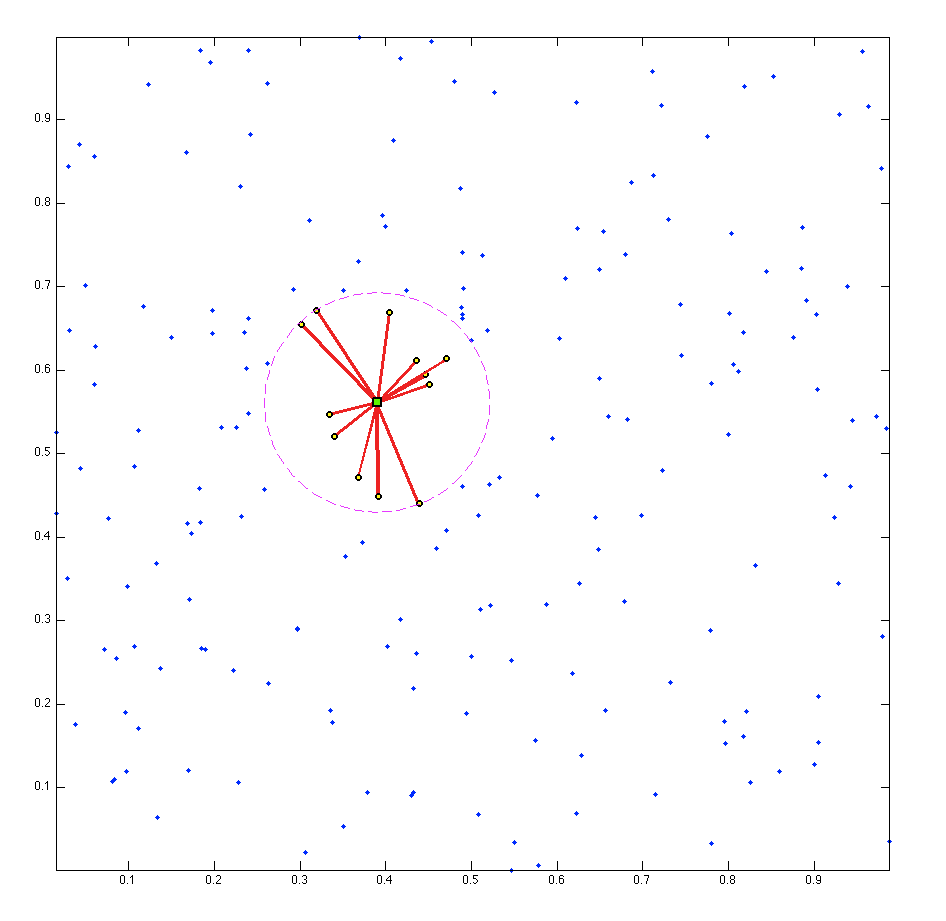
\includegraphics[width=1.0\textwidth]{../figures/chapter1/preview_stencils_example.png}
		\caption{A 13 node RBF-FD stencil of randomly distributed nodes. The stencil centered at the green square contains the 12 nearest neighbors contained within the minimum covering circle drawn in purple.}
		\label{fig:stencil_example_random}
	\end{subfigure}
	\begin{subfigure}[m]{0.35\textwidth}
		\centering
		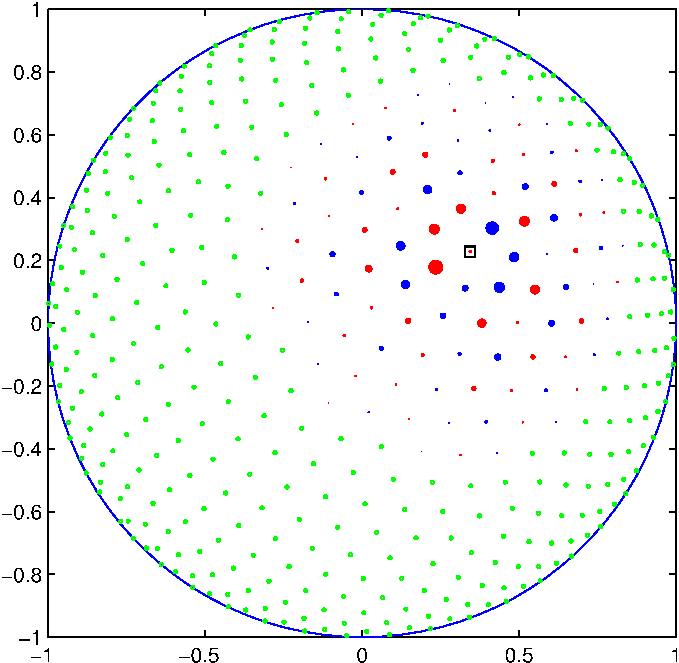
\includegraphics[width=1.0\textwidth]{../figures/chapter1/RBFFD_single-eps-converted-to.pdf}
		\caption{A 75 node RBF-FD stencil with blue (negative) and red (positive) differentiation weights to approximate advective operator at the square. Stencils weights indicated by scale of disk radii. (Image courtesy of Bengt Fornberg and Natasha Flyer)}
		\label{fig:stencil_example_sphere}
	\end{subfigure}
	\caption{Examples of stencils computable with RBF-FD}
	%TODO: Consider: show example FD stencil (5pt with regular grid)
	\label{fig:stencil_example}
\end{figure}

Figure~\ref{fig:stencil_example} provides two examples of RBF-FD stencils. First, Figure~\ref{fig:stencil_example_random} illustrates a single stencil of size $n=13$ in a domain of randomly distributed nodes. The stencil center, $x_c$, is represented by a green square, with the 12 neighboring nodes connected via red edges. The purple circle, the minimum covering circle for the stencil, demonstrates that the stencil contains only the 12 nearest neighbors of the center node. In Figure~\ref{fig:stencil_example_sphere}, a larger RBF-FD stencil of size $n=75$ on the unit sphere is shown as red and blue disks surrounding the center represented as a square. Green disks are nodes outside of the stencil. The radii and color of the red and blue disks represent the magnitude and alternating sign of coefficients, $c_j$, determined to calculate a derivative quantity at the stencil center. 

%TODO: stencil does not need to be regular distribution.
%One of the most appealing benefits of RBF-FD is its built-in support for irregular and unstructured node distributions. 





% The center node and its neighbors define a \emph{stencil}, $\{\vx\}_{i=1}^{n}$, in a localized (small) region or \emph{neighborhood} of the domain. 


%TODO: Weights for both classical Finite Difference and RBF-FD can be obtained through the solution of linear systems. In the case of Finite Difference, the system is a Vandermonde matrix. 
%TODO: For RBF-FD the system is based on a symmetric distance matrix. 
%TODO: Need better description and ref The key difference between FD and RBF-FD systems is the singularity that occurs when two nodes swap.

\subsection{Stencil Weights} 

 To approximate $\diffop{u(x)}$, one requires the stencil \emph{weights} (coefficients), ${c_j}$. Stencil weights are a discrete representation of the differential operator at the stencil center and may vary by node location (e.g., nodes at the boundary are usually governed by another operator, $\boundop$). Weights are obtained by enforcing that they be exact within the space spanned by the RBFs centered at stencil nodes (i.e., $\phi_j(x) = \phi(\epsilon ||x-x_j||_2)$; an RBF centered at $x_j$). Various studies  \cite{WrightFornberg06,FornbergDriscoll02,FornbergLehto11,FlyerLehto11} show that better accuracy is achieved when the 
interpolant can exactly reproduce a constant, $p_0$, such that	\begin{align*}
	       \left. \diffop{\phi_i(x)} \ \right|_{x=x_c} = \sum_{j=1}^{n} c_j \phi_j(x_i) + c_{n+1} p_0 \ \ \ \ \ \ \textrm{for }i=1,2,...,n  
	\end{align*}
	with $\diffop{\phi}_i$ provided by analytically applying the differential operator to the RBF. Assuming $p_0 = 1$, the constraint $\sum_{i=1}^{n}c_i=\diffop{p_0}|_{x=x_{c}}=0$ completes the system: 
	\begin{eqnarray}        
          \begin{bmatrix} \phi_1(x_1) & \phi_2(x_1) & \cdots & \phi_n(x_{1}) & 1 \\ 
            \phi_1(x_2) & \phi_2(x_2) & \cdots & \phi_n(x_{2}) & 1\\ 
            \vdots & \ddots & \ddots & \vdots & \vdots \\ 
            \phi_{1}(x_n) & \phi_{2}(x_n) & \cdots & \phi_{n}(x_{n}) & 1 
            \\ 1 & 1 & \cdots & 1 & 0 \end{bmatrix} 
            \begin{pmatrix} c_1 \\ c_2 \\ \vdots \\ c_n \\ c_{n+1} \end{pmatrix} & = & \begin{pmatrix} \left.\diffop{\phi_1}(x)\ \right|_{x=x_c} \\  \left.\diffop{\phi_2}(x)\ \right|_{x=x_c} \\ \vdots \\  \left.\diffop{\phi_{n}}(x)\ \right|_{x=x_c} \\ 0 \end{pmatrix} \label{eq:rbffd_weight_system} \\
\begin{bmatrix} \phi & P \\
		P^T & 0 \end{bmatrix} \begin{pmatrix} c_\diffop{} \\ 
							d_\diffop{} \end{pmatrix} & = & \begin{pmatrix} \phi_{\diffop{}} \\
							0 \end{pmatrix}. \nonumber
	\end{eqnarray}	
The choice of $\diffop{}$ can be any linear operator. As an example, if $\diffop$ is the identity operator, then the above procedure leads to RBF-FD weights for interpolation. If $\diffop=\pd{}{x}$, one obtains the weights to approximate the first derivative in $x$. Refer to \cite{Fasshauer2007} for a table of commonly used RBF derivatives. Section~\ref{sec:weight_operators} provides a list of derivatives used in this work. 

The small $(n + 1) \times (n + 1)$ system in Equation~\ref{eq:rbffd_weight_system} is dense, and is solved at a cost of $O(n^3)$ floating point operations (FLOPs) using direct methods like LU-decomposition. The resulting stencil weights, $c_\diffop{} = \{c_j\}_{j=1}^n$ can be substituted into Equation~\ref{eq:derivFromFDWeights} for the derivative approximation at $x_c$. Coefficient $c_{n+1}$ ($d_\diffop{} = c_{n+1}$), included in the solution of Equation~\ref{eq:rbffd_weight_system}, is of no use and discarded once the system has been solved. 

Based on the choice of support parameter, $\epsilon$, the Equation~\ref{eq:rbffd_weight_system} may suffer problems with conditioning. In such cases, stable methods like Contour--Pad\'{e} \cite{Wright2003} or RBF-QR \cite{Fornberg2011a,Davydov2011} may be preferred.  


%The above procedure 
%As an example, if $\diffop$ is the identity operator, 
%then the above procedure leads to RBF-FD interpolation. If $\diffop=\pd{}{x}$, one obtains the DM that approximates the first derivative in $x$. 

%TODO: Use of the 1's constraint is highly recommended. It keeps weights within magnitude 100, whereas not providing the constraint results in much higher magnitudes in the thousands or tens of thousands. Using first order monomials does not add benefit. Include examples of weights in 2D with 5 to 10 nodes.

%TODO: weights applied to u
\subsection{Differentiation Matrix}
Note that Equation~\ref{eq:rbffd_weight_system} resolves the weights only for the stencil $x_c$. The small system solve is repeated $N$ times---once for each stencil---to obtain a total of $N \times n$ stencil weights. 

For PDEs, it is common practice to assemble a \emph{differentiation matrix} (DM); a discrete representation of the PDE operator on the domain. Given the set of nodes in the domain $\{x_k\}_{k=1}^N$, the $c$-th row of the DM represents the discrete PDE operator for the stencil centered at node $x_c$ with stencil nodes $\{x_j\}_{j=1}^{n}$: 
\begin{align*}
 \diffop{u(x)} & \approx D_{\diffop{}} u \\
D_\diffop{}^{(c,k)} & = \begin{cases} c_j & x_k = x_j \\
                                    0 & x_k \neq x_j \\
                                    \end{cases} 
\end{align*}
where $(c,k)$ represents the (row, column) index of $D_\diffop{}$ and vector $u = \{u(x_k)\}_{k=1}^{N}$. Equation~\ref{eq:derivFromFDWeights} can be rewritten as:
\begin{align*}
\left. \diffop{u(x)} \ \right|_{x = x_c} & \approx D_{\diffop{}}^{(c)} u \ \ .
\end{align*}
In the solution of PDEs the DMs are utilized in explicit and implicit modes. Here explicit implies evaluating the matrix-vector mulitply to get derivative values, $u'$, from explicitly known vector of solution values $u$: 
\begin{align}
u' = D_{\diffop{}} u
\label{eq:explicit_eq}
\end{align}
whereas implicit solves for unknown $u$:
\begin{align}
D_{\diffop{}} u = f
\label{eq:implicit_eq}
\end{align}

An example RBF-FD DM is illustrated in Figure~\ref{fig:example_DM_rows}. In this example, assume operator $\diffop{} = \pd{}{x}$ is approximated at all $N$ stencil centers of an arbitrary domain. RBF-FD weights assemble the rows of the differentiation matrix, $D_{x}$. On each row, weights are indicated by blue dots. The sparsity of rows reflects the subset of $\{x_k\}_{k=1}^N$ included in corresponding stencils of size $n$. On the right hand side, discrete derivative values $\d{u}{x}$ are approximated at all stencil centers. 

\begin{figure}[htbp]
	\centering
		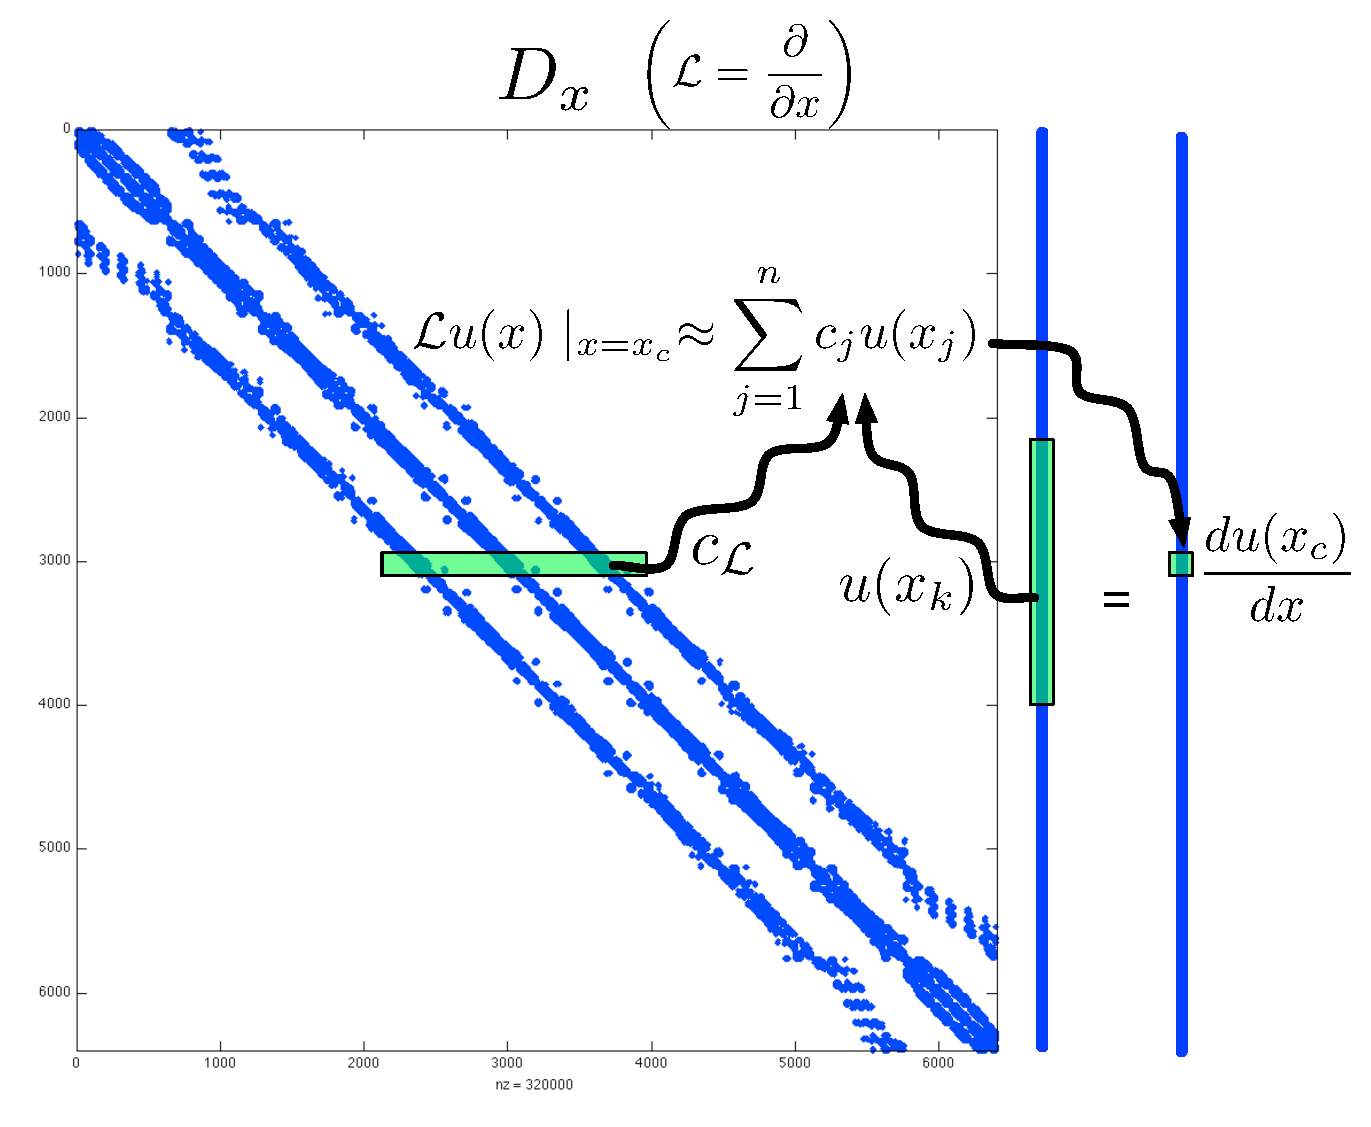
\includegraphics[width=0.65\textwidth]{omnigraffle/DM_rows.pdf}
		\caption{Differentiation matrix $D_x$ is applied to the solution values $u(x)$ to obtain derivative approximations, $\d{u}{x}$. }
		\label{fig:example_DM_rows}
\end{figure}

%TODO: note that DM does not depend on $u(x)$; only x. if the function u(x) wer
Differentiation matrices are assembled at a cost of $O(n^3 N)$ FLOPs. However, since the goal of RBF-FD is to keep stencil neighborhoods small ($n \ll N$), the cost of assembly scales as $O(N)$. Furthermore, RBF-FD weights are independent of function values ($u(x)$) and rely only on stencil node locations. The implications of this are as profound as in the context RBF-PS for time-dependent PDEs: the stencil weights are constant so long as the nodes are stationary. Thus, the DM assembly is part of a one-time preprocessing step.% and can applied explicitly in $O(N)$ operations  

%TODO: verify
% Generally speaking DM application at each time-step scales as $O(N)$ for explicit solutions and $O(N^2)$ for implicit. 

The sparsity exhibited by the DM in Figure~\ref{fig:example_DM_rows} is typical for RBF-FD due to $n \ll N$. 
%A problem of size $N$ with stencil size $n$ results in an $N \times N$ DM with only $N*n$ non-zeros. For $N=10,000$ and $n=31$, roughly $0.3\%$ of the matrix is non-zero, and the percentage only decreases as $N$ increases. 
Best practices dictate that the DMs be stored in a compressed sparse storage format to retain only non-zeros and their corresponding indices in memory. 
%TODO: This reduces the $N^2$ matrix elements to a memory footprint of  

%TODO: storage in sparse rather than dense form
%TODO: storage allows us to precompute and apply at later time-steps. 

%TODO: swapping nodes does not cause singularity



\subsection{Multiple Operators}

In many cases, multiple derivatives (e.g., $\diffop{} = \nabla^2$, $\pd{}{x}$, $\pd{}{y}$, etc.) are required at stencil centers. This is common, for example, when solving coupled PDEs. For RBF-FD, acquiring weights for each additional operator can be both straight-forward and computationally efficient. For each change of differential operator, observe that only the RHS of Equation~\ref{eq:rbffd_weight_system} is modified. Thus, new operators amount to extending Equation~\ref{eq:rbffd_weight_system} to solve 
\begin{eqnarray}
    \begin{bmatrix} \phi & P \\
		P^T & 0 \end{bmatrix} \begin{bmatrix} c_{\nabla^2} & c_{x} & c_{y} & \cdots \\ 
							d_{\nabla^2} & d_{x} & d_{y} & \dots \end{bmatrix} & = &     
		\begin{bmatrix} \phi_{\nabla^2} & \phi_{x} & \phi_{y} & \cdots \\
							0 & 0 & 0 & \cdots \end{bmatrix}. \nonumber
	\end{eqnarray}
where multiple sets of weights ($c_\nabla, c_x, c_y$) are obtained simultaneously. This dense, symmetric, multiple RHS linear system is considered ideal by linear algebra packages, and many highly optimized routines exist to solve them (e.g., LAPACK ``dgesv") \cite{Lapack1999}. 

%TODO: boundaries can be, but are not always handled by special operators
%TODO: preprocessing complexity vs timestep 


\subsection{Weight Operators}
\label{sec:weight_operators}
%Throughout the development of our parallel code we have verified code correctness through the solution of a variety of PDEs.
In the course of this work we work with a variety of PDEs. This section enumerates a list of relevant operators and their corresponding equations for the RHS of Equation~\ref{eq:rbffd_weight_system}. Whenever possible the general form of $\diffop{\phi}$ is provided; otherwise the Gaussian RBF ($\phi(r) = e^{-(\epsilon r)^2}$) is assumed. 

\subsubsection{First and Second Derivatives ($\frac{1}{r}\pd{\phi}{r}, \pdd{\phi}{r}$)}
The following are used in subsequent derviatives:
\begin{align*}
\frac{1}{r}\d{}{r}\phi(r) & = -2 \epsilon^2 \phi(r) \\
\pdd{\phi}{r} & = \epsilon^2(-2 + 4(\epsilon r)^2)\phi(r)
\end{align*}



\subsubsection{Cartesian Gradient ($\grad$)}
The first derivatives in Cartesian coordinates ($\pd{}{x}, \pd{}{y}, \pd{}{z}$) are produced via the chain rule:
	\begin{align*} 
	 \pd{\phi}{x} = \pd{r}{x} \pd{\phi}{r} = \frac{(x-x_{j})}{r} \pd{\phi}{r} \\
	 \pd{\phi}{y} = \pd{r}{y} \pd{\phi}{r} = \frac{(y-y_{j})}{r} \pd{\phi}{r} \\
	 \pd{\phi}{z} = \pd{r}{z} \pd{\phi}{r} = \frac{(z-z_{j})}{r} \pd{\phi}{r}
	\end{align*}
where $\pd{\phi}{r}$ for the Gaussian RBFs is given above. 


\subsubsection{Cartesian Laplacian ($\Laplacian$)}
Fasshauer \cite{Fasshauer2007} provides the general form of $\nabla^2$ in 2D as: 
\begin{align*}
\nabla^2 = \pdd{}{r}\phi(r) + \frac{1}{r}\pd{}{r} \phi(r) 
\end{align*}
For Gaussian RBFs in particular we have the following operators:
\begin{itemize}
\item 1D: $$\nabla^2 = \epsilon^2 (-2 + 4 (\epsilon r)^2) \phi(r)$$
\item 2D: $$\nabla^2 = \epsilon^2 (-4 + 4 (\epsilon r)^2) \phi(r)$$
% e^{-(\epsilon r)^2}$
\item 3D: $$\nabla^2 = \epsilon^2 (-6 + 4 (\epsilon r)^2) \phi(r)$$
% e^{-(\epsilon r)^2}$
\end{itemize}
which all fit $\nabla^2 = \pdd{}{r}\phi(r) + \frac{d - 1}{r}\pd{}{r} \phi(r)$ for dimension $d$.

%
%
%
%2D: \begin{align}
% \nabla^2 = 
% \end{align}
%3D: 
%\begin{align} 
%\epsilon^2 \\
%r^2 \\
%r^2 (\epsilon r)^2 \\
%\nabla^2 = \pd{}{x^2} = 2 \epsilon^2 ( -1 + 2 r^2 ( \epsilon r)^2) \phi(r)
%\end{align}
%
%
%\begin{verbatim}
%                eps2 = ep.^2;
%                xdv = nodes(imat,1) - nodes(imat(1),1);
%                x2eps2 = xdv.^2 * eps2;
%                switch dim
%                    case 1
%                        B(1:n, windx) = 2 .* eps2 .* (-1 + 2.*x2eps2) .* rbf.phi(ep, rdv);
%                    case 2
%                        % Imat is stencil indices
%                        % imat(1) gets stencil center
%                        % ydv = x_i.y - x_j.y
%                        % nodes(imat(1),:) = x_j
%                        ydv = nodes(imat,2) - nodes(imat(1),2);
%                        y2eps2 = ydv.^2 * eps2;
%                        B(1:n, windx) = 4 .* eps2 .* (-1 + x2eps2 + y2eps2) .* rbf.phi(ep, rdv);
%                    case 3
%                        ydv = nodes(imat,2) - nodes(imat(1),2);
%                        zdv = nodes(imat,3) - nodes(imat(1),3);
%                        r2eps4 = (xdv.^2 + ydv.^2 + zdv.^2) * eps2 * eps2;
%                        % r2eps4 = r^2 \epsilon^4
%                        B(1:n, windx) = (-6 .* eps2 + 4 .* r2eps4) .* rbf.phi(ep, rdv);
%\end{verbatim}


\subsubsection{Laplace-Beltrami ($\LaplaceBeltrami$) on the Sphere}

The $\Laplacian$ operator can be represented in spherical polar coordinates for $\mathbb{R}^3$ as: 
\begin{align*} 
\Laplacian = \underbrace{\frac{1}{r} \pd{}{r} \left( r^{2} \pd{}{r}  \right)}_{\mathsf{radial}} + \underbrace{\frac{1}{r^2} \Delta_{S}}_{\mathsf{angular}} , \label{eq:laplacian_in_spherical}
\end{align*}
where $\LaplaceBeltrami$ is the Laplace-Beltrami operator---i.e., the Laplacian operator constrained to the surface of the sphere. This form nicely illustrates the separation of components into radial and angular terms. 

In the case of PDEs solved on the unit sphere, there is no radial term, so we have:
\begin{align}
\Laplacian  \equiv \LaplaceBeltrami.
\end{align}
Although this originated in the spherical coordinate system, \cite{WrightFlyerYuen10} introduced the following Laplace-Beltrami operator for the surface of the sphere: 
\begin{align*} 
\LaplaceBeltrami = \frac{1}{4} \left[ \left(4-r^2\right) \pdd{\phi}{r} + \frac{4-3r^2}{r} \pd{\phi}{r} \right],
\end{align*} 
where $r$ is the Euclidean distance between nodes of an RBF-FD stencil and is independent of our choice of coordinate system. 

\subsubsection{Constrained Gradient ($P_{x} \cdot \grad$) on the Sphere}

Following \cite{FlyerWright09, FlyerLehto11}, the gradient operator can be constrained to the sphere with this projection matrix: 
%\frac{1}{||\mathbf{x}||}
\begin{align}
P = I - \mathbf{x} \mathbf{x}^T =  \begin{pmatrix} 
(1-x_1^2) & -x_1 x_2 & -x_1 x_3 \\
-x_1 x_2 & (1-x_2^2) & -x_2 x_3 \\ 
-x_1 x_3 & -x_2 x_3 & (1-x_3^2) 
\end{pmatrix} = \begin{pmatrix} P_{x_1} \\ P_{x_2} \\ P_{x_3} \end{pmatrix}
\label{eq:project_gradient}
\end{align}
where $\mathbf{x}$ is the unit normal at the stencil center. 


The direct method of computing RBF-FD weights for the projected gradient for $\mathbf{P} \cdot \nabla $ is presented in \cite{FlyerWright09}. When solving for the weights, we apply the projection on the right hand side of our small linear system. We let $\vx = \begin{pmatrix} x_1, x_2, x_3 \end{pmatrix} $ be the stencil center, and $\vx_k=\begin{pmatrix} x_{1,k}, x_{2,k}, x_{3,k}\end{pmatrix}$ indicate an RBF-FD stencil node. 

Using the chain rule, and assumption that 
$$r(\vx_k-\vx)=\vectornorm{\vx_k-\vx} = \sqrt{(x_{1,k}-x_1)^2 + (x_{2,k}-x_2)^2 + (x_{3,k}-x_3)^2},$$
 we obtain the unprojected gradient of $\phi$ as
\begin{align*}
\nabla \phi(r(\vx_k - \vx)) = \pd{r}{\vx} \pd{\phi(r(\vx_k - \vx))}{r} = - (\vx_k - \vx)\frac{1}{r(\vx_k - \vx)} \pd{\phi(r(\vx_k - \vx))}{r} .
\end{align*} 

Applying the projection matrix gives 
\begin{align*}
\mathbf{P} \nabla \phi(r(\vx_k - \vx)) & = - (\mathbf{P} \cdot \vx_k - \mathbf{P}\cdot\vx)\frac{1}{r(\vx_k - \vx)} \pd{\phi(r(\vx_k - \vx))}{r} \\
& =  - (\mathbf{P}\cdot\vx_k - 0)\frac{1}{r(\vx_k - \vx)} \pd{\phi(r(\vx_k - \vx))}{r} \\
& = - (I-\vx\vx^T)(\vx_k
)\frac{1}{r(\vx_k - \vx)} \pd{\phi(r(\vx_k - \vx))}{r} \\
& = \begin{pmatrix} x \vx^T \vx_k - x_k \\ y \vx^T \vx_k -  y_k \\ z \vx^T \vx_k -z_k \end{pmatrix} \frac{1}{r(\vx_k - \vx)} \pd{\phi(r(\vx_k - \vx))}{r} 
 \end{align*}
Thus, we directly compute the weights for $P_{x}\cdot\grad{}$ using these three RHS in Equation~\ref{eq:rbffd_weight_system}: 
\begin{align*} 
P\pd{}{x_1} = ( x_1 \vx^T \vx_k - x_{1,k}) \frac{1}{r(\vx_k - \vx)} \pd{\phi(r(\vx_k - \vx))}{r} |_{\vx=\vx_j} \\
P\pd{}{x_2} = ( x_2 \vx^T \vx_k - x_{2,k}) \frac{1}{r(\vx_k - \vx)} \pd{\phi(r(\vx_k - \vx))}{r} |_{\vx=\vx_j} \\
P\pd{}{x_3} = ( x_3 \vx^T \vx_k - x_{3,k}) \frac{1}{r(\vx_k - \vx)} \pd{\phi(r(\vx_k - \vx))}{r} |_{\vx=\vx_j}
\end{align*}

%TODO: finish appendix
%Alternatively, assuming weights for operators $\grad = \pd{}{x_{1}}, \pd{}{x_{2}}, \pd{}{x_{3}}$ are already computed, the projected operator could be constructed via weighting the unprojected gradient components. For example: 

%\authnote{Show accuracy of derivative approximation when using projected operator vs linear combinations of dx,dy,dz operators}


\subsubsection{Hyperviscosity $\Delta^k$ for Stabilization}

When explicitly solving hyperbolic equations, differentiation matrices encode convective operators of the form 
\begin{equation}
D = \alpha \pd{}{\lambda} + \beta \pd{}{\theta} \label{eqconv}
\end{equation}
%TODO: where $\alpha$ and $\beta$ are a function of the fluid velocity. 
The convective operator, discretized
through RBF-FD, has eigenvalues  
 in the right half-plane causing the method to be unstable~\cite{FornbergLehto11, FlyerLehto11}.  
Stabilization of the RBF-FD method is achieved through the application of a hyperviscosity filter 
to Equation~(\ref{eqconv}) \cite{FornbergLehto11}. By using Gaussian 
 RBFs, $\phi(r) = e^{-(\epsilon r)^2}$, the hyperviscosity (a high order Laplacian operator) simplifies to
\begin{equation}
\Delta^{k}\phi(r) = \epsilon^{2k} p_k(r) \phi(r)
\label{eqn:gaussian_hv}
\end{equation}
where $k$ is the order of the Laplacian and  $p_k(r)$ are multiples of generalized Laguerre polynomials that
are generated recursively (\cite{FornbergLehto11}):
\begin{align*}
\begin{cases} 
p_0(r) &=1, \\
p_1(r) &= 4(\epsilon r)^2 - 2d, \\
p_k(r) &= 4((\epsilon r)^2 - 2(k-1) - \frac{d}{2})  p_{k-1}(r) - 8(k-1)(2(k-1) - 2 + d) p_{k-2}(r), \ \ \ \ k = 2, 3, ...
\end{cases}
\end{align*}
where $d$ is the dimension of the problem. The application of hyperviscosity in Chapter~\ref{chap:explicit_implicit_pdes}, utilizes the operator as a filter to shift eigenvalues and stabilize advection equations on the surface of the unit sphere. In that case, $d=2$ is assumed ksince individual RBF-FD stencils can be viewed as (nearly) lying on a plane. For small $N$, the diameter of the stencil may not be sufficiently 
small compared to the radius of the sphere, and hyperviscosity might not work as advertised. 
%However,
%numerical evidence in \cite{FornbergLehto11,BolligFlyer} \ci suggests that if the RBFs adequately resolve the convective operator, the 2D 
%hyperviscosity operator does its job. 
%We base our work on the work of Fornberg and Lehto \cite{FornbergLehto11}, which was
%performed on a sphere, and tune our parameters following their guidelines. 

In the case of parabolic and hyperbolic PDEs, hyperviscosity is added as a filter to the right hand side of the evaluation. For example, at the continuous level, 
the equation solved takes the form
\begin{equation}
\pd{u}{t} = - \diffop u + H u,
\label{eq:evaluation_with_hyperviscosity}
\end{equation}
where $\diffop$ is the PDE operator, and $H$ is the hyperviscosity filter operator.
Applying hyperviscosity shifts all the eigenvalues of $L$ (the discrete form of $\diffop{}$) to the left half of the complex plane. 
This shift is controlled by $k$, the order of the Laplacian, and a scaling parameter $\gamma_c$, defined by
\begin{equation*}	
H = \gamma \Delta^{k} = \gamma_c N^{-k} \Delta^{k}.
\end{equation*}
It was found in \cite{FlyerLehto11}, and verified in our own application, that $\gamma = \gamma_c N^{-k}$  provides stability and good accuracy for all values of $N$ considered here. It also ensures that the viscosity vanishes as $N\rightarrow\infty$ \cite{FlyerLehto11}.
In general, the larger the stencil size, the higher the order of the Laplacian.  This is attributed to the fact that, for convective operators, larger stencils treat a wider range of modes accurately. As a result, the hyperviscosity operator should preserve as much of that range as possible. The parameter $\gamma_c$ must also be chosen with care and its sign depends on $k$ (for $k$ even, $\gamma_c$ will be negative and for $k$ odd, it will be positive). If $\gamma_c$ is too large, the eigenvalues move outside the stability domain of our time-stepping scheme and/or eigenvalues corresponding to lower physical modes are not left intact, reducing the accuracy of our approximation. If $\gamma_c$ is too small, eigenvalues remain in the right half-plane \cite{FornbergLehto11,FlyerLehto11}.


%TODO: sparsity
%TODO: Node ordering
%TODO: show blocks for boundary conditions (annulus)
%TODO: application (explicit/implicit solution)

\section{Implementation}

This section provides an overview of how one implements RBF-FD. Consider Algorithm~\ref{alg:rbffd_high_level}. The algorithm is partitioned into two phases: preprocessing and application. The complexity of each phase depends on the choice of algorithms/method utilized for each task. 

Preprocessing encompasses tasks such as grid setup/generation, stencil generation and stencil weight calculations. As output from these tasks one expects one or more DMs representing the discrete differential operators. Assuming the grid nodes do not move, the DMs remain constant for the duration of the second phase. Additionally, DMs can be loaded from disk on subsequent runs to effectively bypass the cost of all preprocessing. 


\begin{algorithm}                      
\caption{A High-Level View of RBF-FD}          
\label{alg:rbffd_high_level}                           
\textbf{Preprocessing:}
\begin{algorithmic}[0]                   
    \State $\{x\}_{j=1}^N$ = GenerateGrid()
   	\For {$j = 1$ to $N$} \label{alg:stencil_gen} 
   	    \State Stencil $\{S_{j,i}\}_{i=1}^{n}$ = QueryNeighbors($x_j$)
   	\EndFor
    \For {$j = 1$ to $N$} \label{alg:weight_calc} 
   	    \State $\{w_{j,i}\}_{i=1}^{n} = $ SolveForWeights($\{S_j\}$)
   	    \State $D_{\diffop{}}^{(j)} = $ AssembleDM($\{w_j\}$)     
    \EndFor
    \algstore{myalg}    % Store the algorithm number count
\end{algorithmic}
\textbf{Application:}
\begin{algorithmic}[1] 
\algrestore{myalg}      % continue to count from store line
    \State $t = t_{min}$                
    \While{ $t < t_{max}$ }
        \State $\{u'\} =$ SolvePDE($D_{\diffop{}}$, $\{u\}$)
        \State $\{u\} =$ UpdateSolution($\{u\}$, $\{u'\}$, $\Delta t$)
        \State $t$ += $\Delta t$
    \EndWhile
\end{algorithmic}
\end{algorithm}


The constructed DMs are applied in the Application phase to solve a PDE either explicitly or implicitly. Note that regardless of the explicit or implicit method, this phase reduces to a Sparse Matrix-Vector Multiply (SpMV) within the SolvePDE step. For explicit solutions, SolvePDE computes the SpMV in Equation~\ref{eq:explicit_eq}. In the implicit case, SolvePDE must invert the DM in Equation~\ref{eq:implicit_eq} via a direct or iterative linear system solve. In the case of time-dependent PDEs, RBF-FD is applied the same as any other finite difference method within a time-stepping scheme (represented by UpdateSolution). % (e.g., Runge-Kutta, Adams-Bashforth, etc.) may require multiple applications of the DM, with the outputs weighted and combined within UpdateSolution. 

Tuning the performance of RBF-FD requires one to focus on the Application phase. This is especially true for time-dependent PDEs where an increase in grid size results in proportional increase in the number time-steps. The recurring cost of computing an SpMV each time-step quickly amortizes the one-time cost of preprocessing. 
 
On the other hand, preprocessing tasks have more impact on accuracy, stability and conditioning of the method. As each of these properties improve, the overall time to solution can decrease thanks to larger stable time-steps, smaller required grid size, and faster convergence (i.e., fewer iterations) within iterative linear system solves.

Here we discuss various design decisions in implementing the preprocessing tasks for RBF-FD and consider potential impacts on performance (if any).  Chapter~\ref{chap:rbffd_multi_gpu} will discuss Application and SpMV performance in more detail. 

\subsection{Grid} 

An implementation of RBF-FD begins with the grid. The method has no requirement for structured grids, or for a well-refined mesh/lattice that limits connectivity between nodes. It operates both on structured grids and random point clouds; although, the choice of grid does impact the accuracy of the method. This freedom to function on domains of any shape, dimension, and granularity is a major selling point for RBF-FD and often impossible for many other PDE methods. 
%Typically, the only constraint placed on the grid is that nodes should not coincide. If two nodes do coincide it is possible for a stencil to include both, and 

%TODO: cubed, ying-yang
% For example classic Finite Difference and many Finite Volume methods operate on regular/Cartesian grids. When operating on the sphere, it is common to encounter Cubed-spheres \cite{TODO:NairJablonowski08} and/or Ying-Yang grids in attempts to bypass the need for small time-steps and to alleviate troubling pole singularities common to Latitude/Longitude grids \cite{TODO}. Generalizations to unstructured meshes 
% TODO: Discontinuous Galerkin? How deep do I want to go?
%are possible for many methods (e.g., Finite Volume on multi-resolution \cite{RinglerJuGunzberger2008}) and Finite Element methods \cite{TODO}, but such methods still have a strong dependence on a Delaunay Triangulation or other mesh to determine the connectivity between nodes. 

The choice of grid is only relevant to the extent that it impacts the connectivity between nodes in stencils. Connectivity translates to non-zeros in rows of the DMs, so the various grid distributions result in a number of sparsity patterns. For all other intents and purposes, the choice of grid is only pertinent to ensure consistency with the PDEs to solve. 

In the course of this work, we applied RBF-FD to a number of PDEs and grid distributions. Here we focus on the subset utilized in Chapters~\ref{chap:explicit_implicit_pdes} and \ref{chap:benchmarks}. This subset is chosen for two reasons: a) to easily construct refinements in 2D/3D for consistent benchmarking and convergence studies, and b) to verify our solutions against existing methods. 

%In Chapter~\ref{chap:explicit_implicit_pdes} we test the performance of our method with application to transient and steady-state PDEs. For the purpose of verification we demonstrate convergence for sets of grids previously published in the RBF literature. We briefly describe each type of grid and when it is used. 

\subsubsection{Regular Grid}
For basic debugging and benchmarking purposes the most natural choice is to start with a regular or Cartesian grid. Equally spaced nodes in multiple dimensions are simple to generate. Additionally, refinements---for convergence tests---are direct subsamples. 

In theory, RBF-FD functions the same whether nodes are uniformly spaced or random. However, regular grids do not fully exercise advantages that RBF-FD has over other methods with its ability to operate on scattered nodes.


\subsubsection{Maximum Determinant Nodes}

In Chapter~\ref{chap:explicit_implicit_pdes} we verify our RBF-FD implementation by solving PDEs on the unit sphere. For consistency with respect to related investigations (e.g., \cite{Fornberg2009a, Fornberg2007,FornbergLehto11}), we choose the Maximum Determinant (MD) node sets \cite{Womersley2001, Sloan2003}. %TODO: need ref Womersley2001

MD node sets were introduced to the RBF community due to their success in spherical harmonics interpolation, where the seemingly irregular node distributions gain an order of magnitude accuracy compared to regular looking (Minimum Energy) node distributions \cite{Womersley2001}. RBF interpolation tends to reproduce spherical harmonics interpolants on the sphere when $\epsilon \rightarrow 0$, and RBF methods have been shown to benefit similarly from a subtle irregularity in node locations \cite{Fornberg2007}. 

\begin{figure} 
\centering
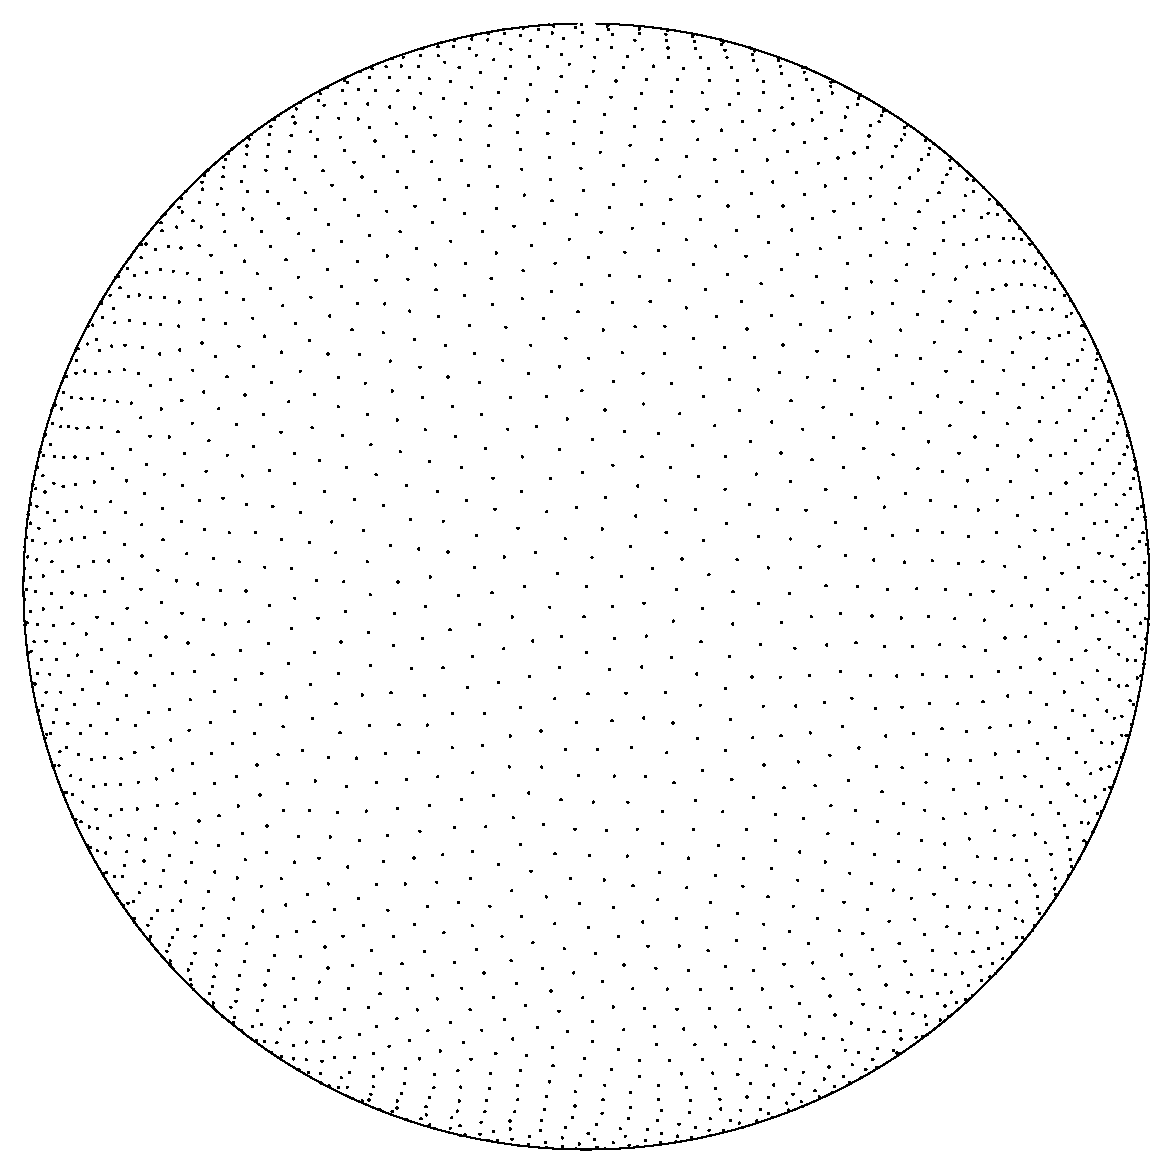
\includegraphics[width=0.4\textwidth]{rbffd_methods_content/grids/N4096_points.pdf} 
\caption{Example of $N=4096$ maximum determinant (MD) node sets on the unit sphere.} 
\label{fig:md_nodes}
\end{figure}

The MD node files are available for download on the authors' web site (\url{http://web.maths.unsw.edu.au/~rsw/Sphere}), and range in size from $N=4$ up to N=27,556 nodes on the sphere. Figure~\ref{fig:md_nodes} plots the $N=4096$ node set to illustrate the irregularity in distribution. Node sets greater than N=27,556 are not available. Unlike regular grids, each MD node set is a refinement of the sphere, but not a subdivision, so extending beyond N=27,556 nodes would require complete regeneration.

%The process of generating new MD node sets greater than $N=27,556$ nodes would require recomputing the entire distribution. 


\subsubsection{Centroidal Voronoi Tessellations}

While the MD nodes suffice for verification against related work, our objective is to scale RBF-FD to problem sizes never attempted. To this end, we sought approximately regular grids on the sphere on the order of hundreds of thousands and even millions of nodes. To this end we leverage Spherical Centroidal Voronoi Tessellations (SCVTs) to generate approximately regular node distributions on the sphere \cite{Du2003b, Womeldorff2008}. 

SCVTs come with a sense of ``optimality" in node locations due to energy minimizing properties \cite{Du2003b}. The process to generate SCVTs involves constructing a Voronoi diagram, computing the mass centroids for each Voronoi partition, and updating node locations to the mass centroids projected onto the sphere. After a number of iterations the nodes coincide with the projected mass centroids and a converged SCVT is produced. In most large-scale applications, this iterative process leverages a probabilistic Lloyd's method, where integrals to compute mass centroids are approximated through random sampling \cite{Womeldorff2008, Du2003b}. While SCVTs in theory converge to a regular node distribution, the probabilistic nature of the centroid calculation introduces irregularities in distribution reminiscent of MD nodes. 

\begin{figure} 
\centering
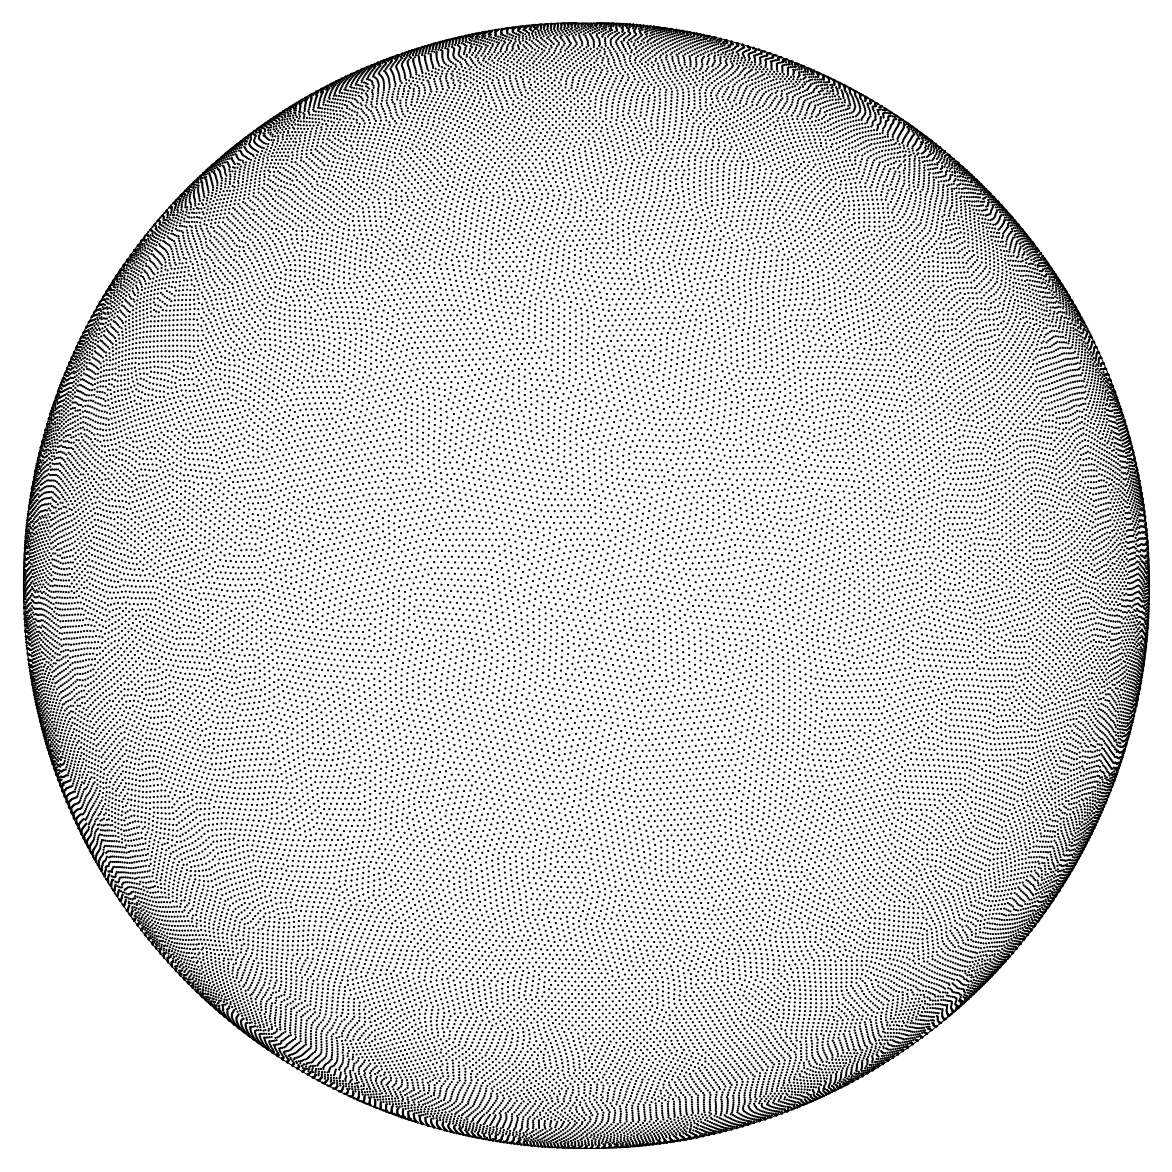
\includegraphics[width=0.4\textwidth]{rbffd_methods_content/grids/N100000_points.png}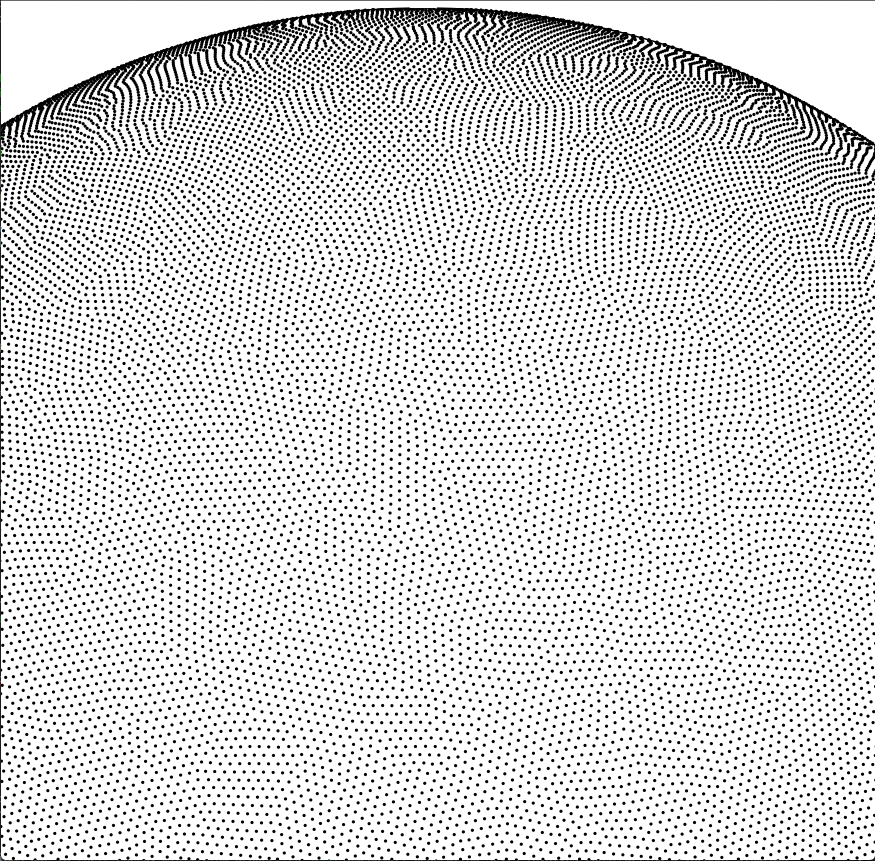
\includegraphics[width=0.4\textwidth]{rbffd_methods_content/grids/N100000_closeup.png} 
\caption{(Left) N=100,000 Spherical Centroidal Voronoi Tessellation nodes. (Right) Close-up of the same N=100,000 nodes to illustrate the irregularities in the grid.} 
\label{fig:scvt_nodes}
\end{figure}

Figure~\ref{fig:scvt_nodes} provides an example SCVT grid with N=100,000 nodes. On the left, the full sphere; on the right, a close-up of the same node set. The close-up perspective clearly demonstrates the random artifacts/scarring of irregularly distributed nodes. For benchmarking purposes we use node sets N=100,000, N=500,000 and N=1,000,000 generated by the SCVT library from \cite{Womeldorff2008}. These SCVT grids are publicly available from: \url{https://github.com/bollig/sphere_grids.git}.

%Not considered here: it is possible to refine grids using density functions in the calculation of the mass centroids. 



%% TODO: mention other grids generated with CVTs and provide examples 
%\subsubsection{Other Grids}
%
%% TODO: wanted to test without the presence of boundary conditions 
%% TODO: other grids tested boundary conditions
%
%While not discussed in detail in this work, various attempts to leverage Centroidal Voronoi Tessellations have been made in our investigation of RBF-FD. Figures~\ref{fig:cvt_other} were used to generate other complex geometries such as the 3D sphere shell, 2D annulus, ellipse and ellipsoid, 
%
%Other grids considered during the thesis, but not included in the applications below: 
%
%\begin{itemize}
%\item Anulus
%\item Nested Sphere CVT
%\item a
%\end{itemize}

\chapter{Generating Stencils for RBF-FD}
\label{chap:stencils}

TODO:
\begin{itemize}
\item Finish KDTree description
\item Hashing neighbor query algorithm description
\item Cite refs on multi-dim spatial data structures
\item Complexity of algorithms
\item impact from ordering on matrix sparsity. Bandwidth impact. Bandwidth impact on condition considered in future chapter. 
\item what is best overlay resolution? based on time to generate. choose resolution as n/2, n/9? etc? 
\item perform neighbor queries on raster order because its easiest to jump cells. then each cell can be reordered according to z,x,u, etc. for better memory locality. Matlab script to do this (can be ported to C)
\end{itemize}

With a grid present, stencils are generated by querying $n$ neighbors for each $N$ total nodes in the domain. While not required, one typically assumes a stencil of $n$ nodes must be the nearest neighbors to a stencil center. Afterall, as the distance between stencil nodes and the stencil center decreases, the accuracy of derivatives increases. 

Brute force searching for neighbors---computing the distance between every pair of nodes and then selecting the $n$ nearest---is discouraged due to its $O(N^2)$ complexity. Common practice in the RBF community is to construct $k$D-Trees to decrease the cost of queries (e.g., \cite{Fasshauer2007, FlyerLehto11, FornbergLehto11}). 

\authnote{Incomplete here to end of section}

Many algorithms exist to query the $k$-nearest neighbors (equivalently all nodes in the minimum/smallest enclosing circle). Some algorithms overlay a grid similar to Locality Sensitive Hashing and query such as... \cite{HarPeledMazumdar2003}.

RBF-FD is designed to handle irregular node distributions. Therefore, it is not essential that stencils contain only nearest neighbors. Instead, one can acquire the \emph{approximate nearest neighbors}. Figure~\ref{fig:ann_example} demonstrates a case where a does not contain all nearest neighbors. As illustrated in the Figure, the ANN stencil and true nearest neighbor stencil differ by one node. THis is not dire



Leveraging $k$D-Trees involves two costs: a) the initial tree construction, and b) $k$-nearest neighbor queries. 

GPU version of Locality Sensitive Hashing could reduce complexity further \cite{Pan2011}

This can be done efficiently using neighbor query algorithms or spatial partitioning data-structures such as Locality Sensitive Hashing (LSH) and $k$D-Tree. Different query algorithms often have a profound impact on the DM structure and memory access patterns. We choose a Raster ($ijk$) ordering LSH algorithm \cite{Bollig2011} leading to the matrix structure in Figures~\ref{fig:oneThreadPerStencil} and \ref{fig:oneWarpPerStencil}. While querying neighbors for each stencil is an embarrassingly parallel operation, the node sets used here are stationary and require stencil generation only once. Efficiency and parallelism for this task has little impact on the overall run-time of tests, which is dominated by the time-stepping. We preprocess node sets and generate stencils serially, then load stencils and nodes from disk at run-time. In contrast to the RBF-FD view of a static grid, Lagrangian/particle based PDE algorithms promote efficient parallel variants of LSH in order to accelerate querying neighbors at each time-step \cite{Pan2011, Goswami2010}. 


At the onset of our work on RBF-FD, the most commonly used KDTree implmentation used by the RBF community was \cite{Tagliasacchi2008}. Recently, improvements were made to the KDTree algorithm to reduce the cost of building the KDTree to $O(N log^2 N)$. 

Figure~\ref{fig:stencil_query_old_and_new} compares the total time to generate $N$ stencils of size $n=50$ with three methods: \cite{Tagliasacchi2008}, our hash-based neighbor query, and the improved KDTree from \cite{Tagliasacchi2012}. 
Until the new release of KDTree, our algorithm was a major improvement to the performance of stencil generation. The hash-based approach achieved greater than 


RBF-FD operates on general node distributions. Historically, stencils are uniform in size ($n$) and generated by selecting the $(n-1)$ true nearest neighbors to a node $x_c$. This is a $k$-NN query. 

Alternative queries are possible: ball query and approximate nearest neighbor. The approximate is of particular interest because nodes closest to the stencil will always be selected, whereas the nodes further away have minimal influence so swapping out cant hurt. The justification in altering the selection is for reduced complexity in neighbor queries.  

%RBF methods are traditionally described as general and meshless in that they apply to unstructured clouds of points in arbitrary dimensions. However, although the term meshless implies a method capable of operating with no node connectivity, all numerical methods---meshless RBF methods included---connect nodes in the domain. For example, the ``meshless'' global RBF method connects every node in the domain to all other nodes. Compact support or local RBF methods like RBF-FD limit connections to nodes that lie within a predetermined radius.

%The connections between nodes form a directed adjacency graph with edges that dictate the paths along which data/phenomena can travel. For example, a plus shaped stencil of five points with a center node and four neighboring nodes allows values to propagate north, south, east and west; not northeast, southeast, etc.


%They are robust and function on scattered point clouds. RBF-FD in particular requires stencils to be generated from $n$ nearest neighbors to a stencil center. The cost of these neighbor queries can vary greatly depending on the choice of algorithm or data-structure used to make the query. 

For example, in general brute force is inefficient 
The author of \cite{Fasshauer2007} queries $n$ nearest neighbors for a compact-support RBF partition of unity example with a $k$-D tree. In \cite{FlyerLehto11,FornbergLehto11} a $k$-D Tree is leveraged for all neighbor queries for RBF-FD. 

Our work in \cite{BolligFlyerErlebacher2012} leveraged an alternative to $k$-D tree, based loosely on space-filling curve orderings common in Lagrangian schemes like Smoothed Particle Hydrodynamics (e.g., \cite{IanThesis}, \cite{Kelager}). %TODO: I have used Locality Sensitive Hashing \cite{Indyk} in the past. According to Samet \cite{Samet "Multidimensional and Metric..."}, LSH uses a set of random hashes to assign indices for each node. Our case uses space-filling curve, so we use . 

Rather than iterate through all $N$ nodes to find the true neighbors, or step through a k-D tree in something like $O(log N)$ that requires extra built-out, ANN allows us to use a set of nodes that satisfy


\begin{figure}
\centering
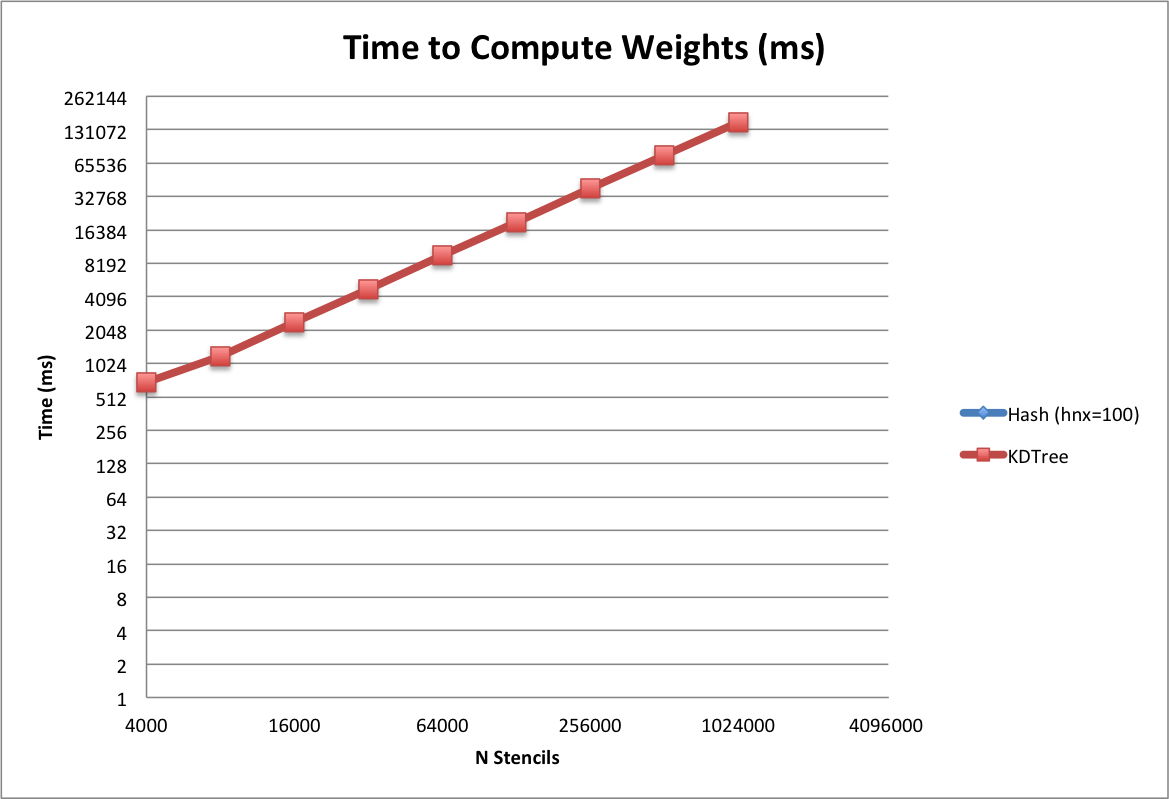
\includegraphics[width=6.5cm]{../figures/stencils/computeWeights_hash_vs_kdtree_hnx100.png}
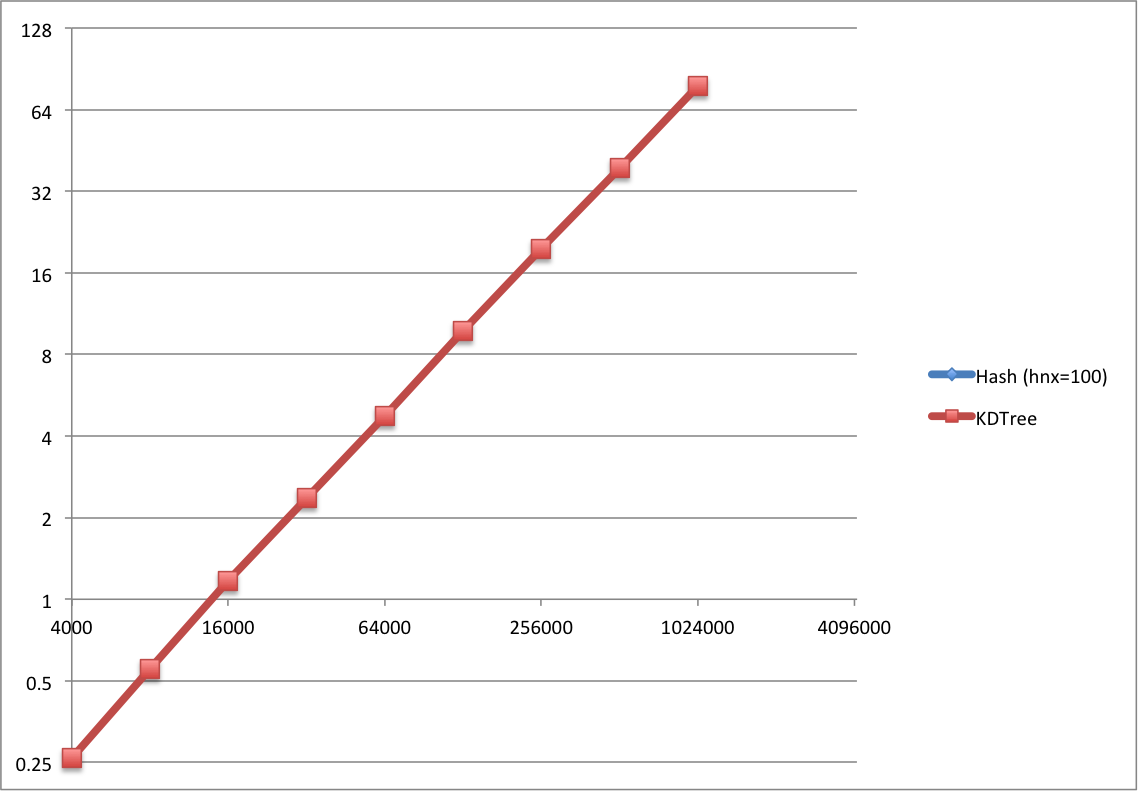
\includegraphics[width=6.5cm]{../figures/stencils/SpMV_hash_vs_kdtree_hnx100.png} \\
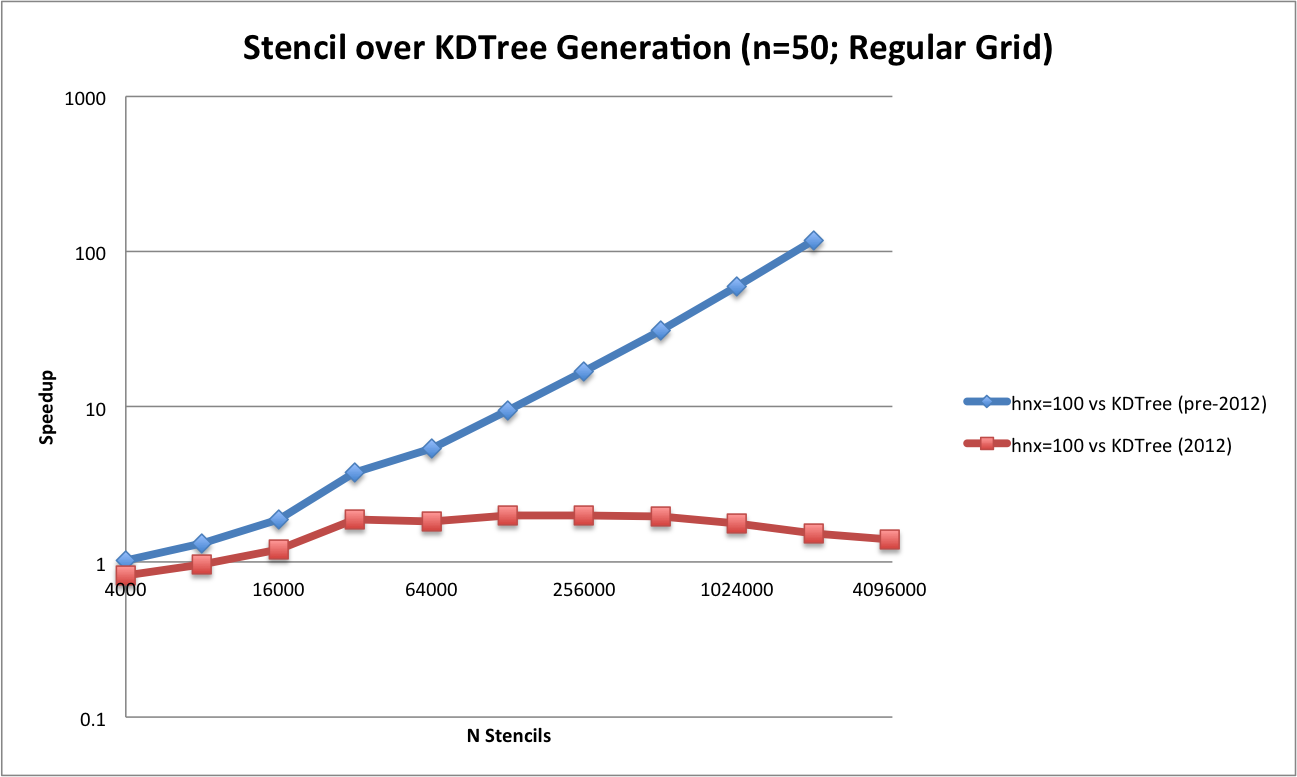
\includegraphics[width=6.5cm]{../figures/stencils/speedup_hash_vs_kdtree_hnx100.png}
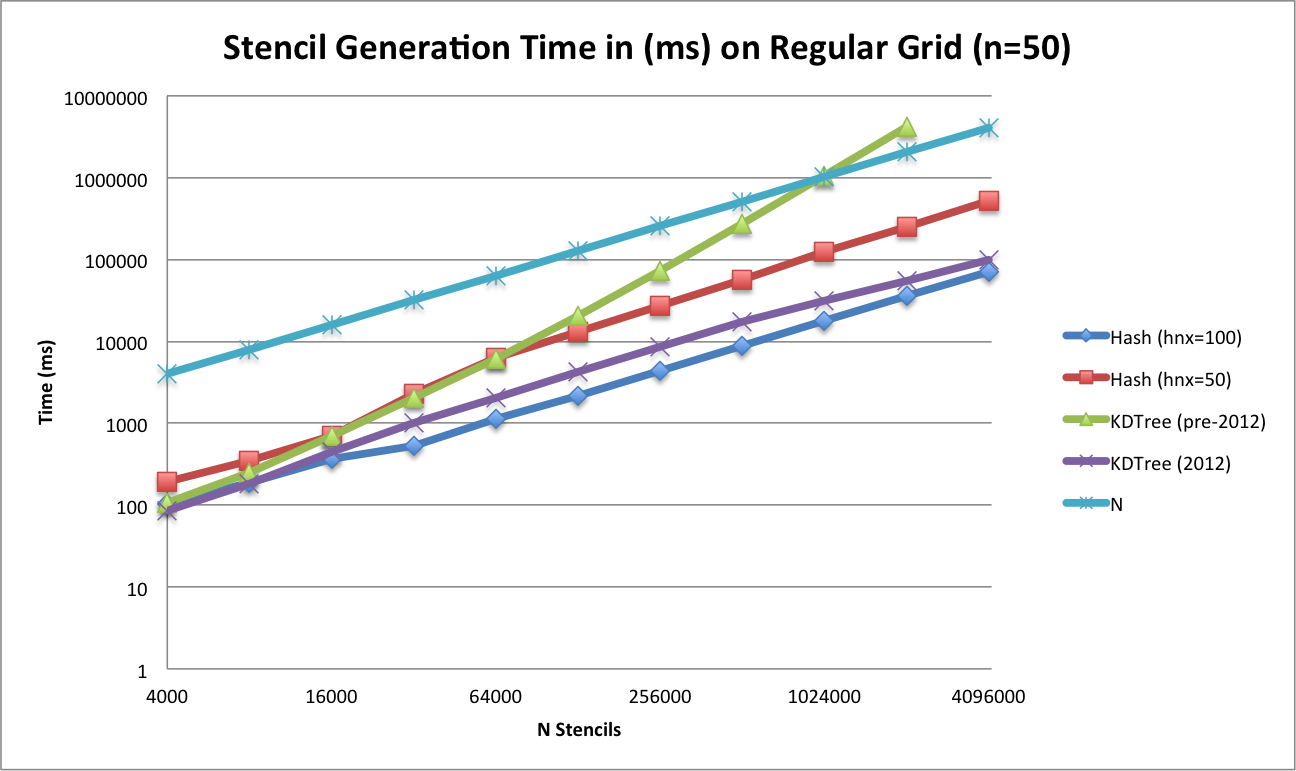
\includegraphics[width=6.5cm]{../figures/stencils/hash_vs_kdtree_hnx100_w_kdtree_new.png} \\
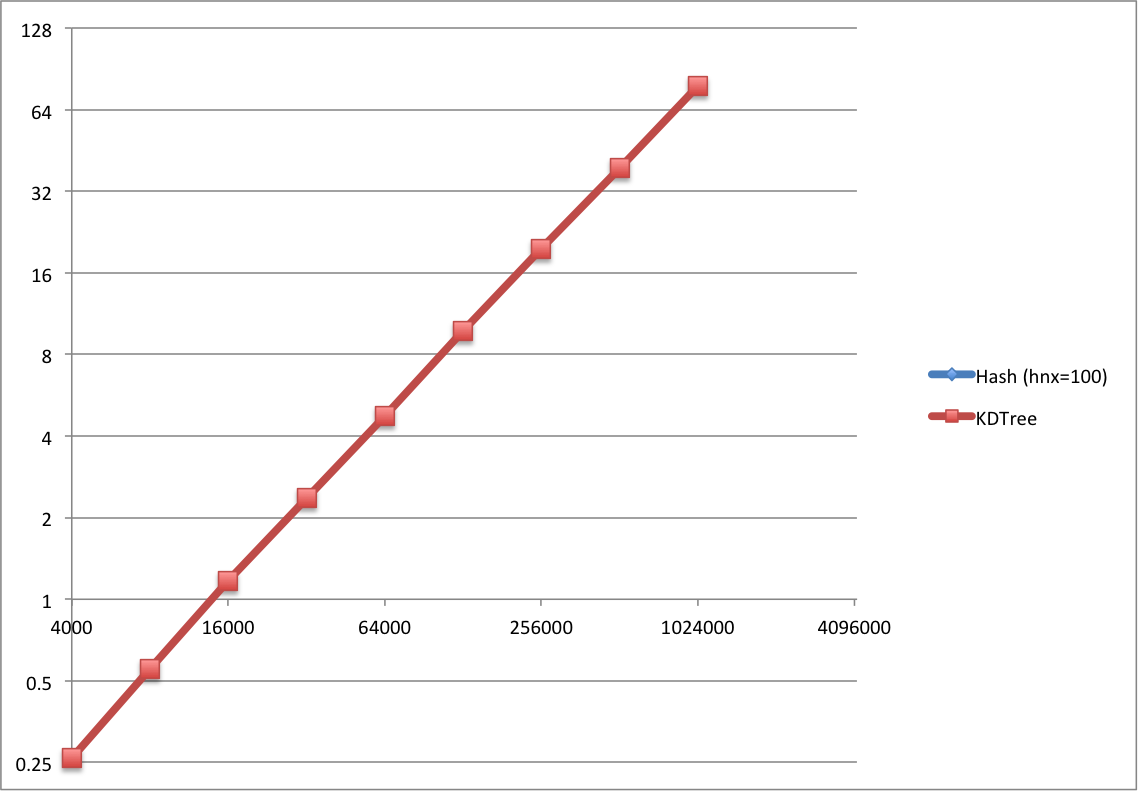
\includegraphics[width=6.5cm]{../figures/stencils/SpMV_hash_vs_kdtree_hnx100.png}
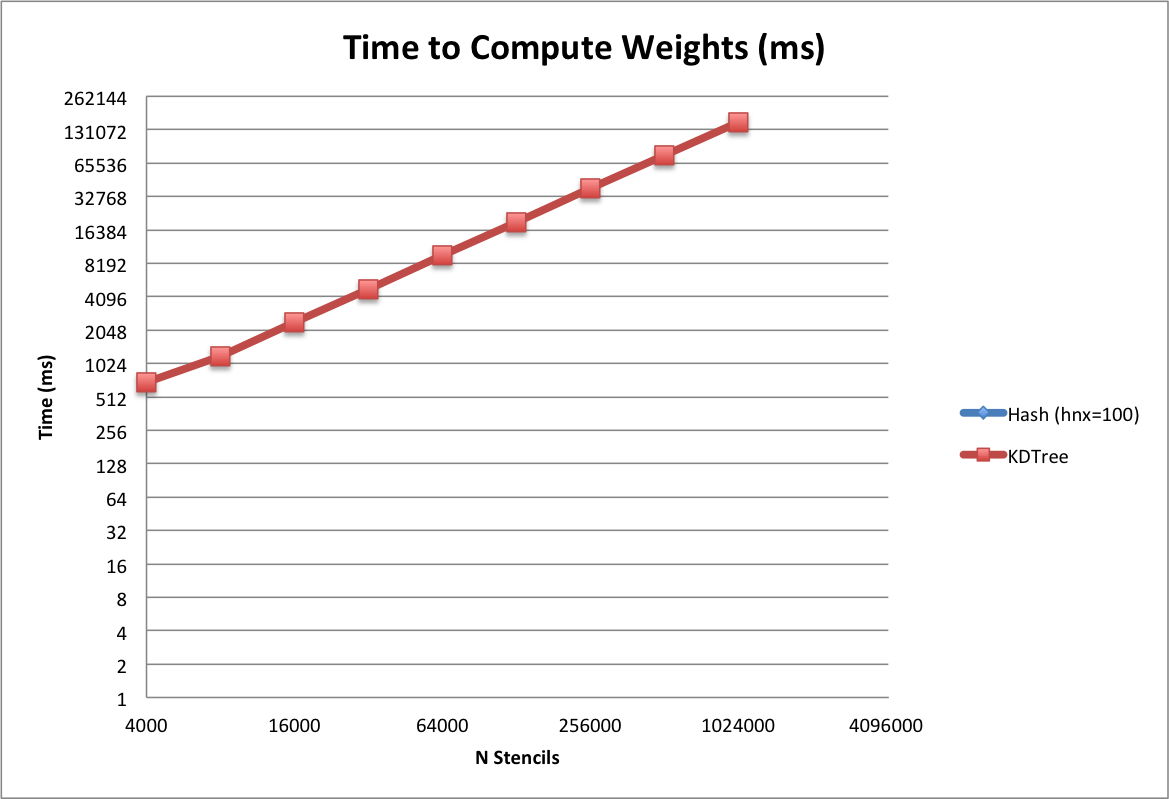
\includegraphics[width=6.5cm]{../figures/stencils/computeWeights_hash_vs_kdtree_hnx100.png} \\
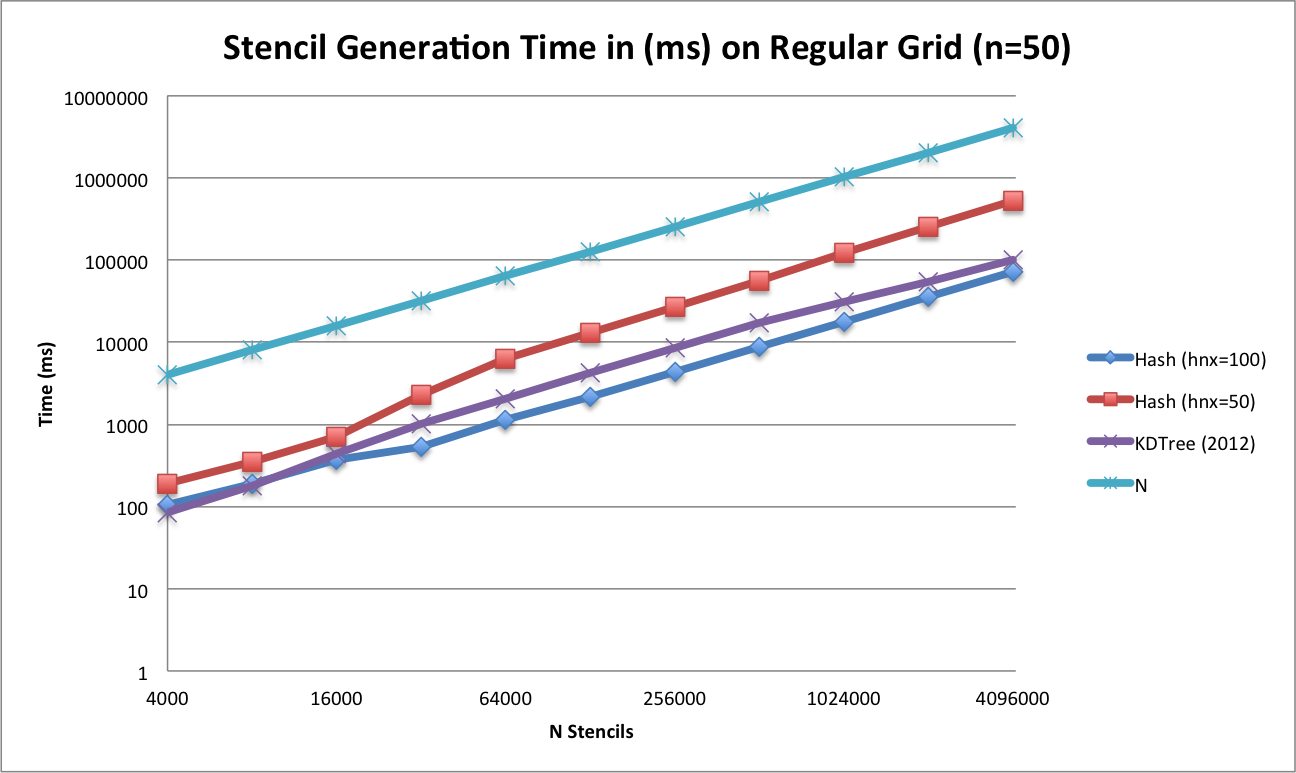
\includegraphics[width=6.5cm]{../figures/stencils/hash_vs_kdtree_hnx100.png}
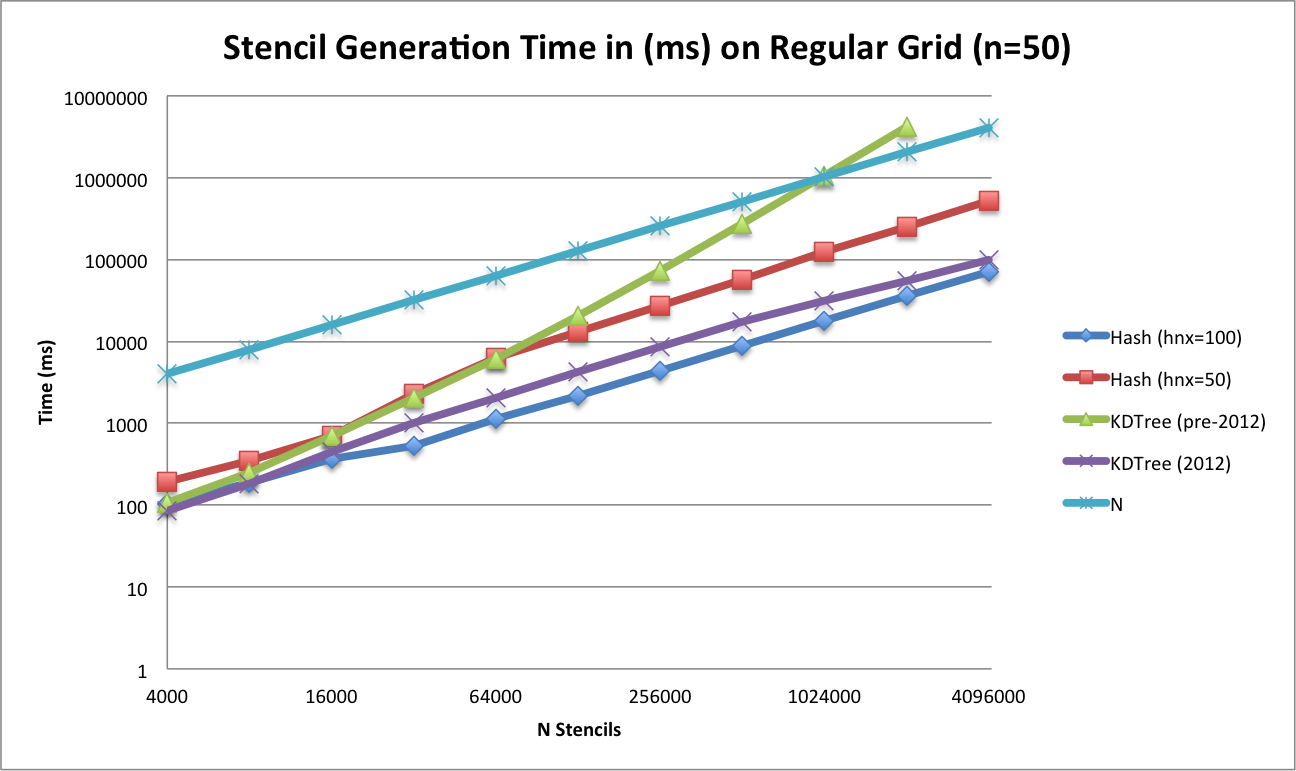
\includegraphics[width=6.5cm]{../figures/stencils/hash_vs_kdtree_hnx100_w_kdtree_new.png} \\
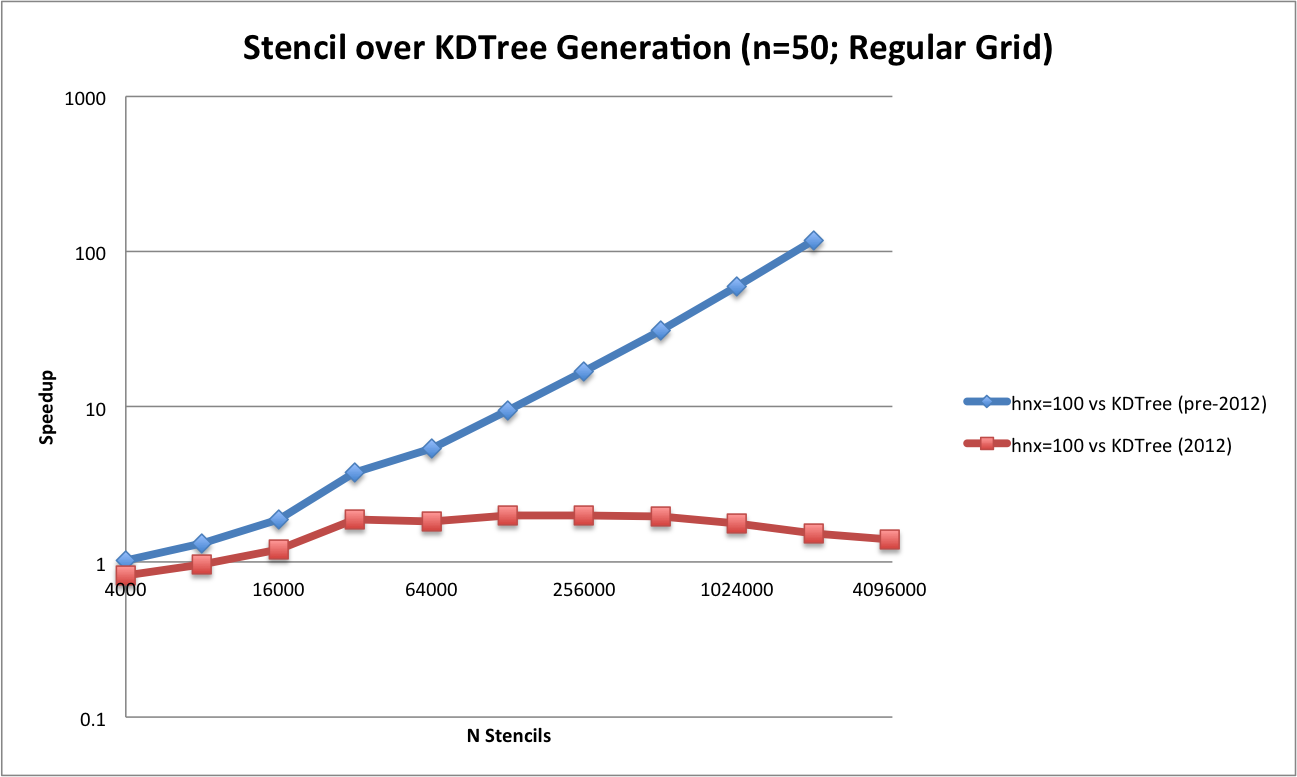
\includegraphics[width=6.5cm]{../figures/stencils/kdtree_old_reg_subsets_4m_stencil_gen_speedup.png}
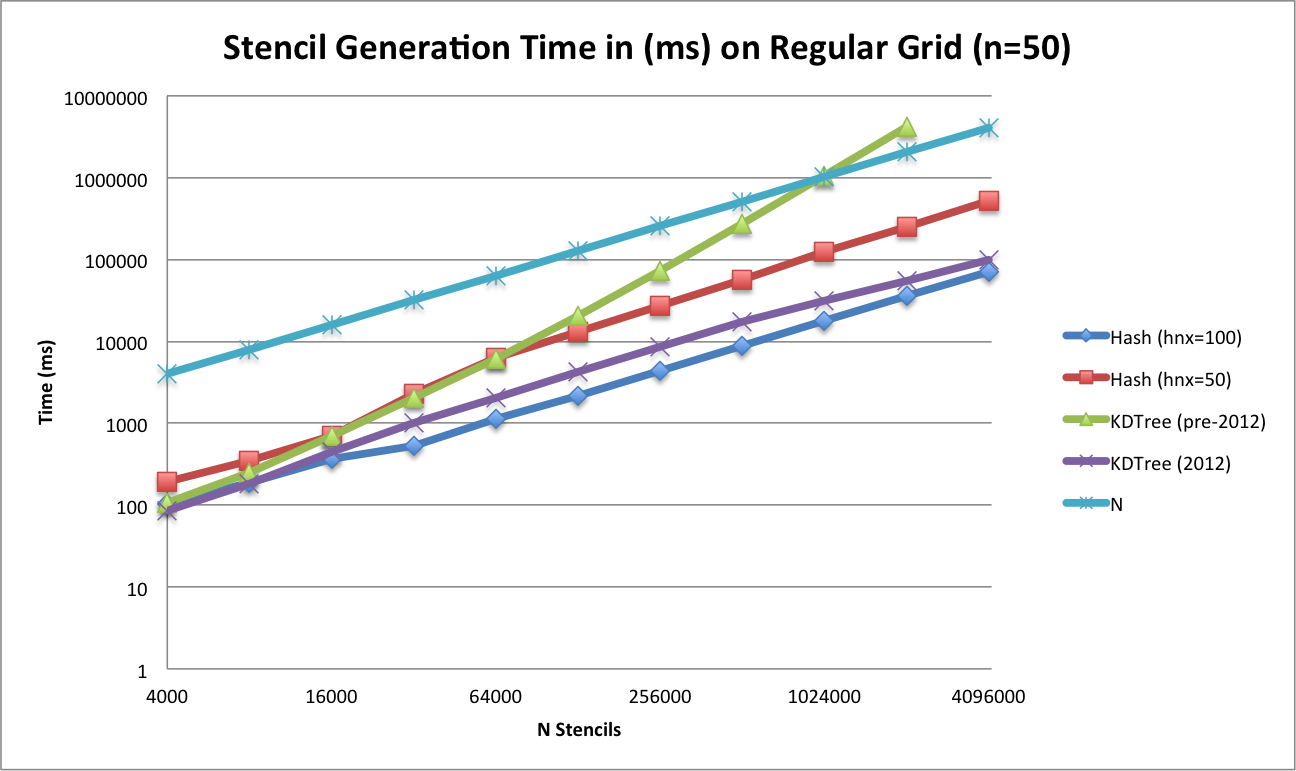
\includegraphics[width=6.5cm]{../figures/stencils/kdtree_old_reg_subsets_4m_stencil_gen_time.png} \\
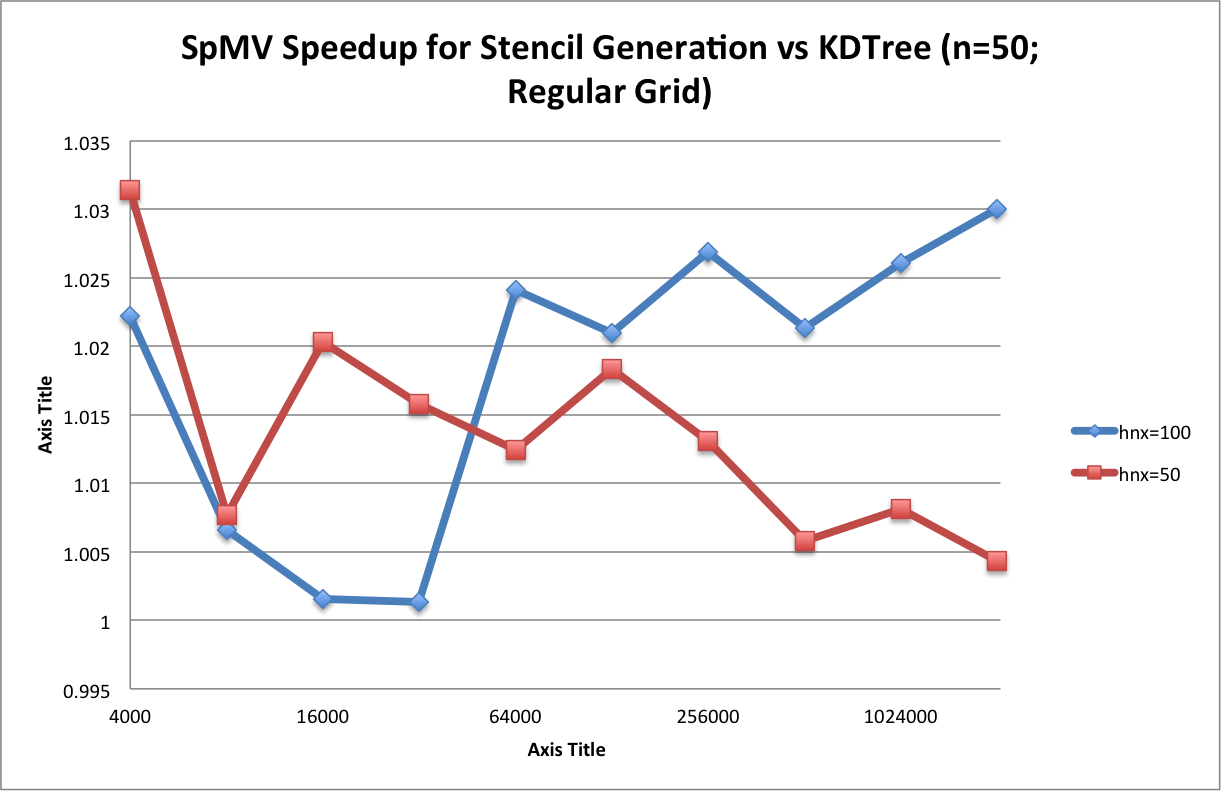
\includegraphics[width=6.5cm]{../figures/stencils/reg_subsets_2m_spmv_speedup.png}
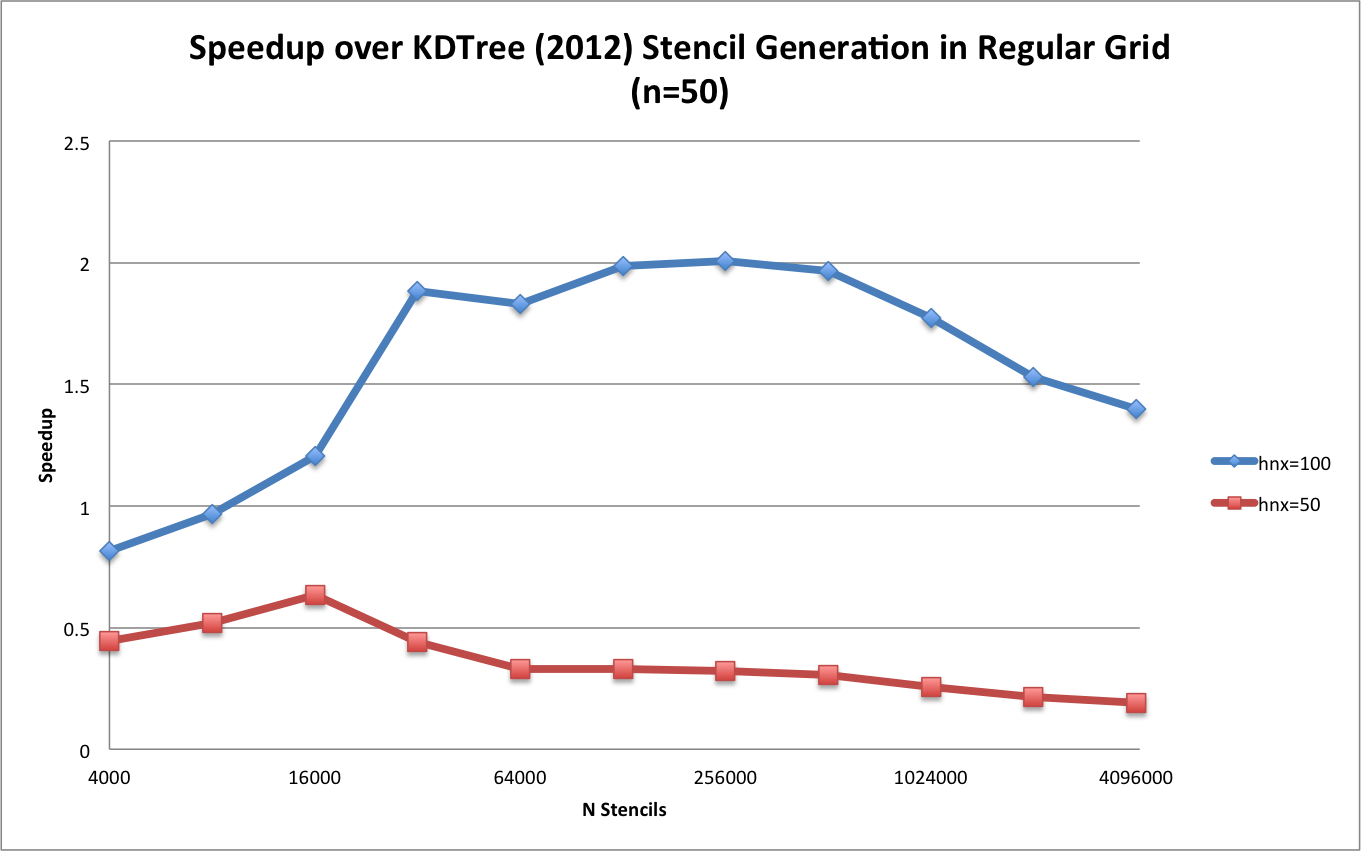
\includegraphics[width=6.5cm]{../figures/stencils/reg_subsets_4m_stencil_gen_speedup.png} \\
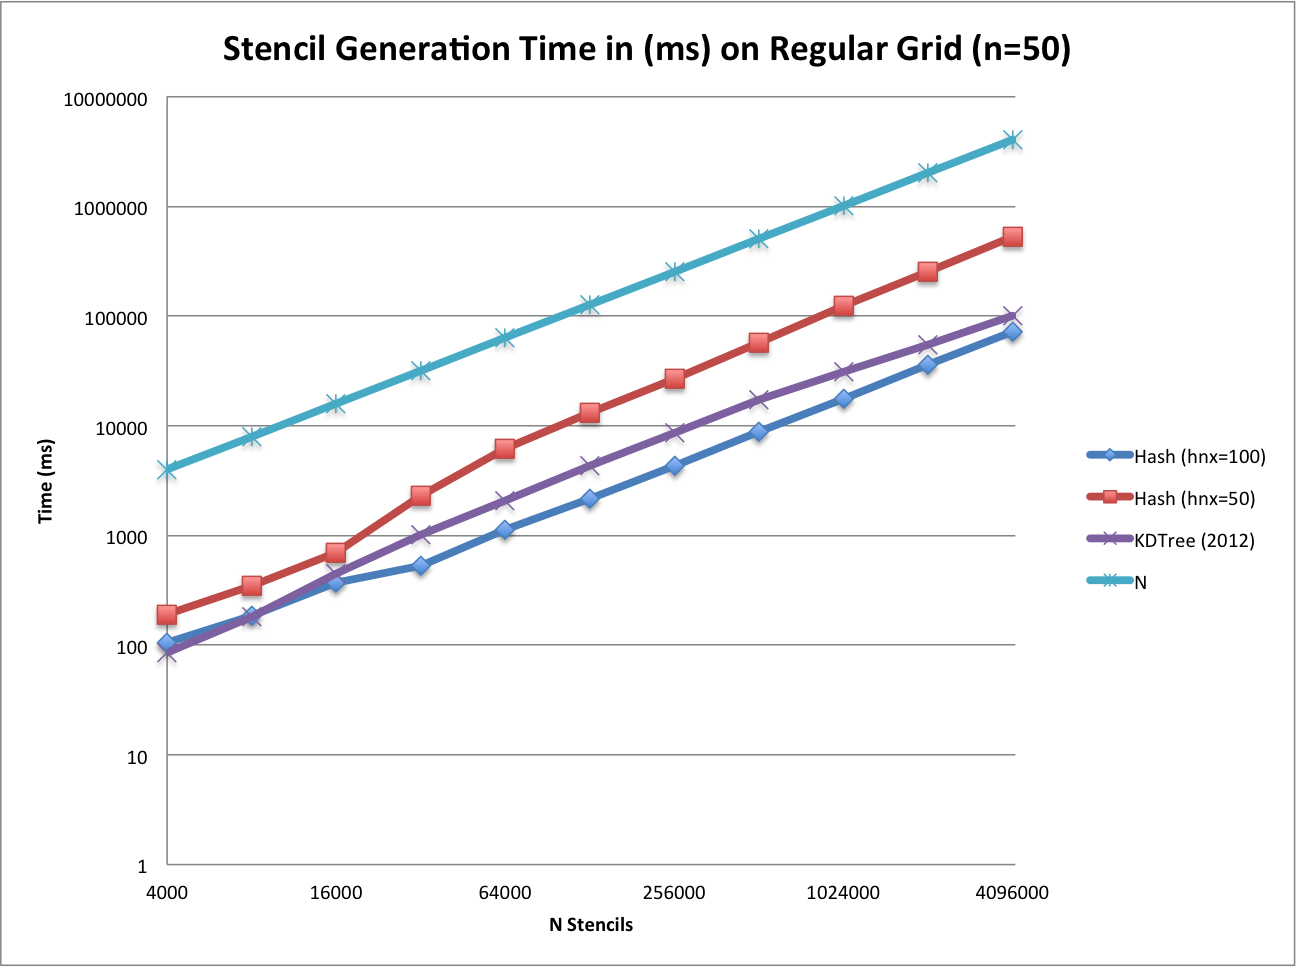
\includegraphics[width=6.5cm]{../figures/stencils/reg_subsets_4m_stencil_gen_time.png}
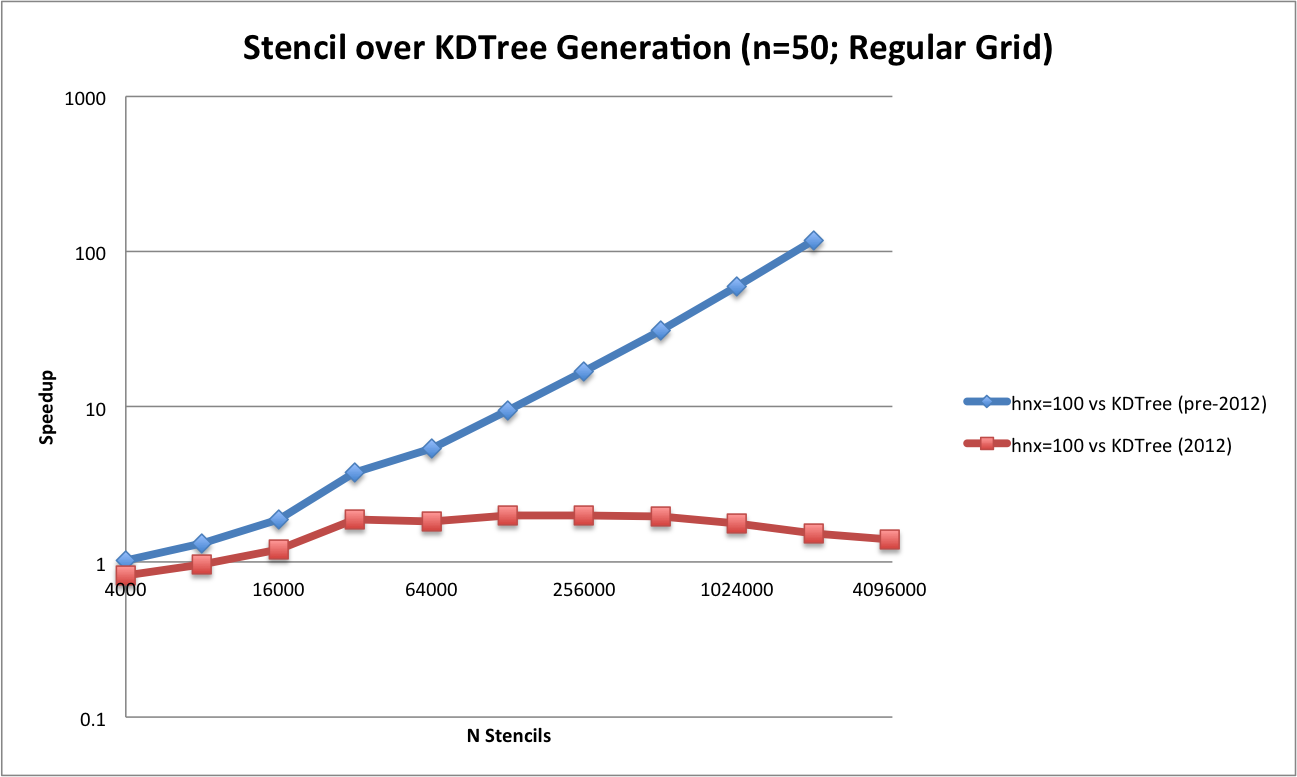
\includegraphics[width=6.5cm]{../figures/stencils/speedup_hash_vs_kdtree_hnx100.png} \\
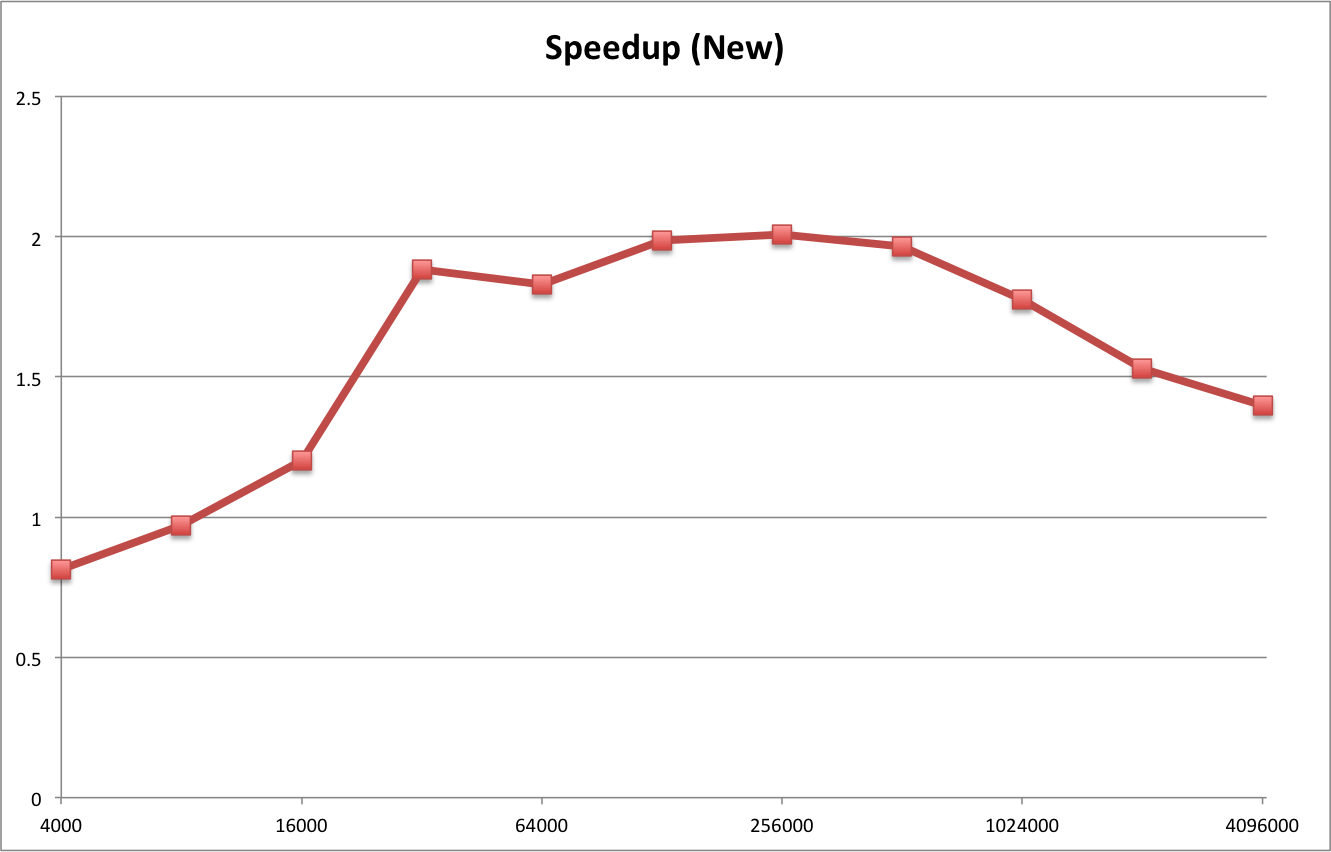
\includegraphics[width=6.5cm]{../figures/stencils/speedup_hnx100_vs_kdtree_new.png}
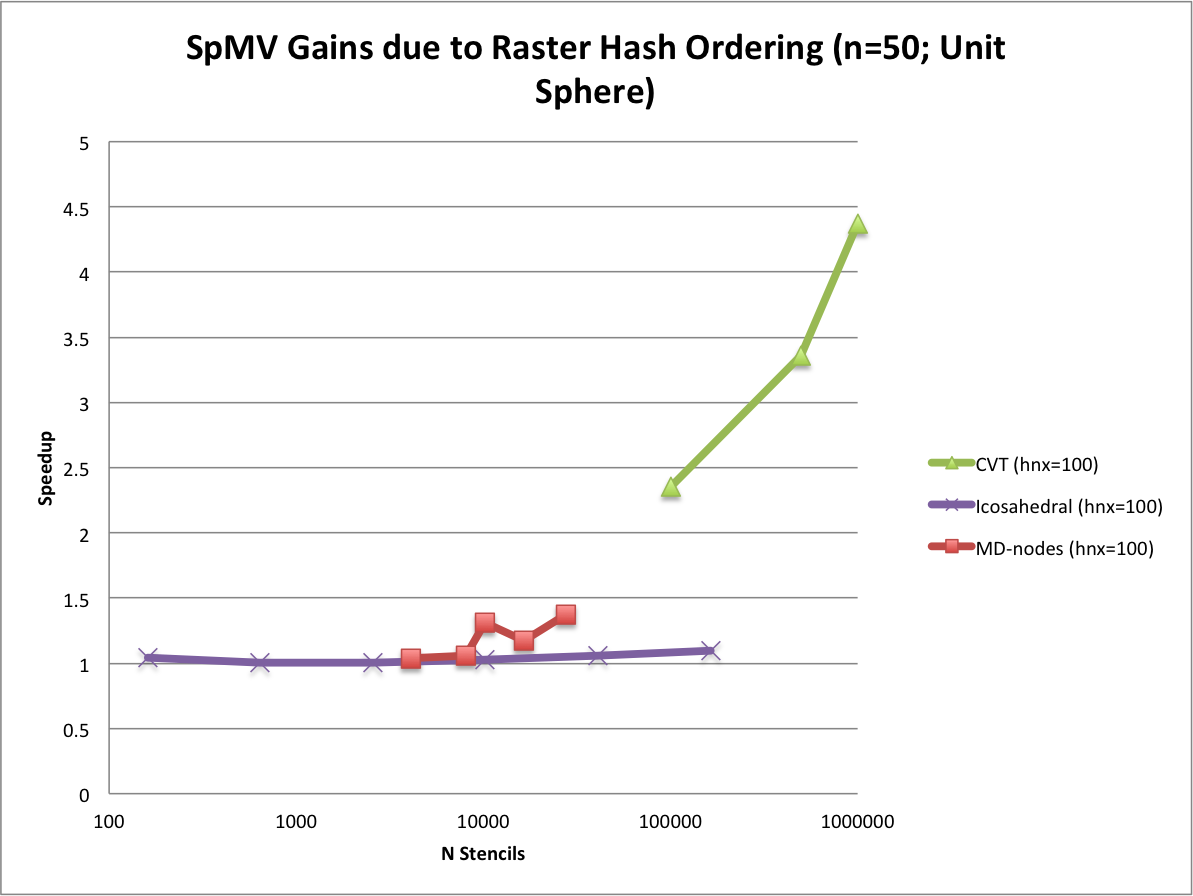
\includegraphics[width=6.5cm]{../figures/stencils/sphere_spmv_speedup.png} \\
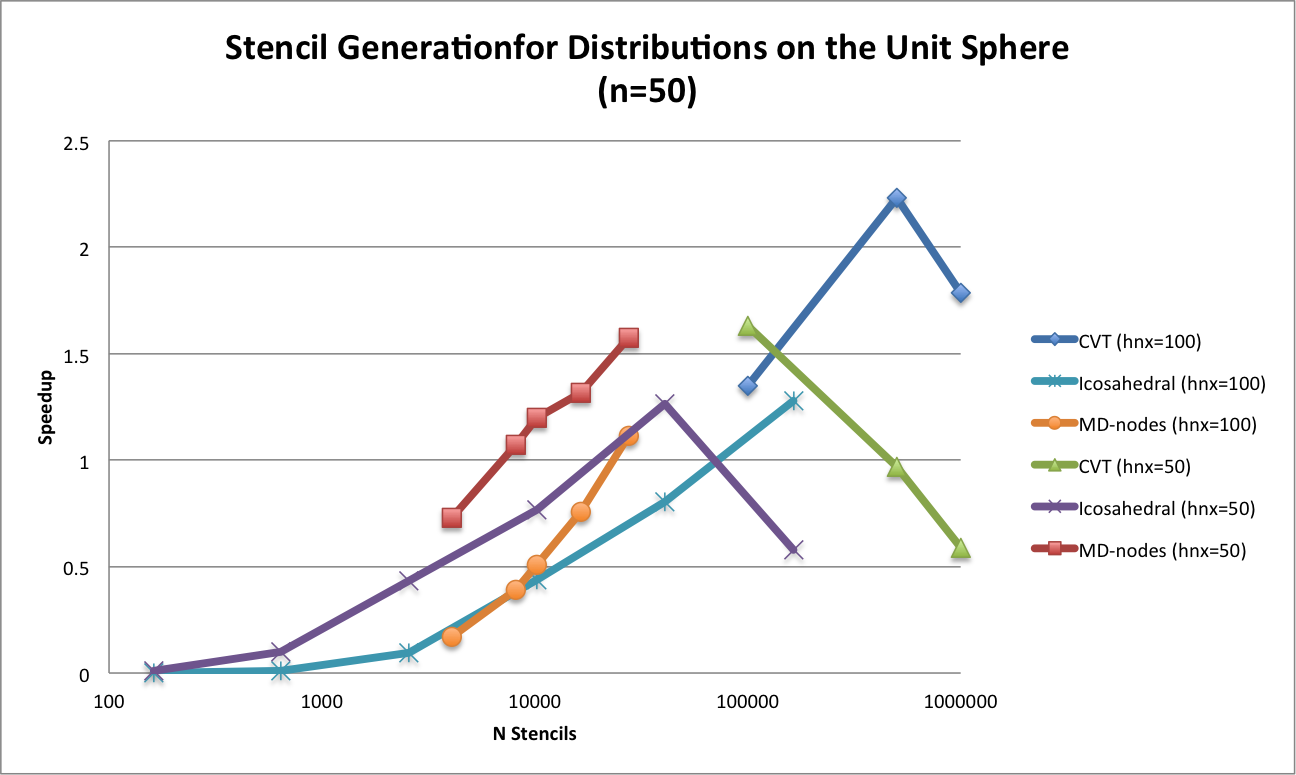
\includegraphics[width=6.5cm]{../figures/stencils/sphere_stencil_gen_speedup.png}
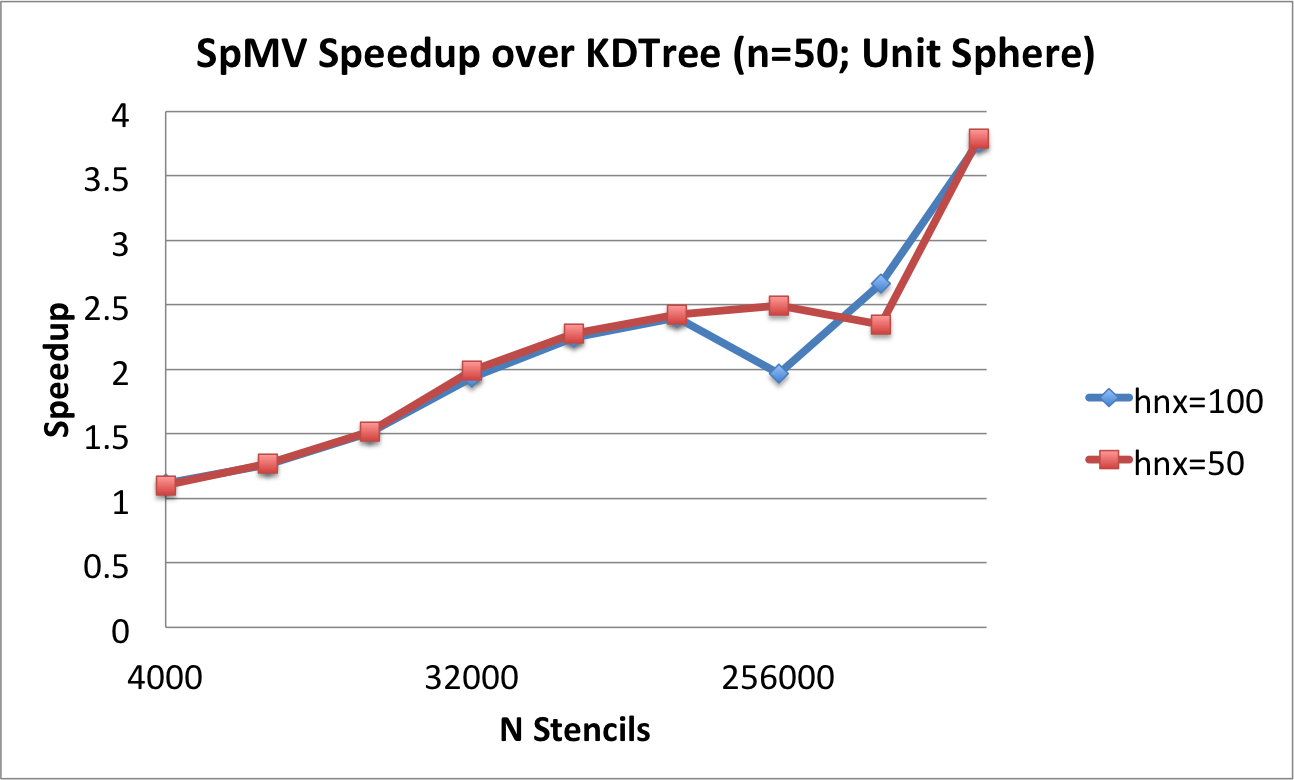
\includegraphics[width=6.5cm]{../figures/stencils/sphere_subsets_1m_spmv_speedup.png} \\
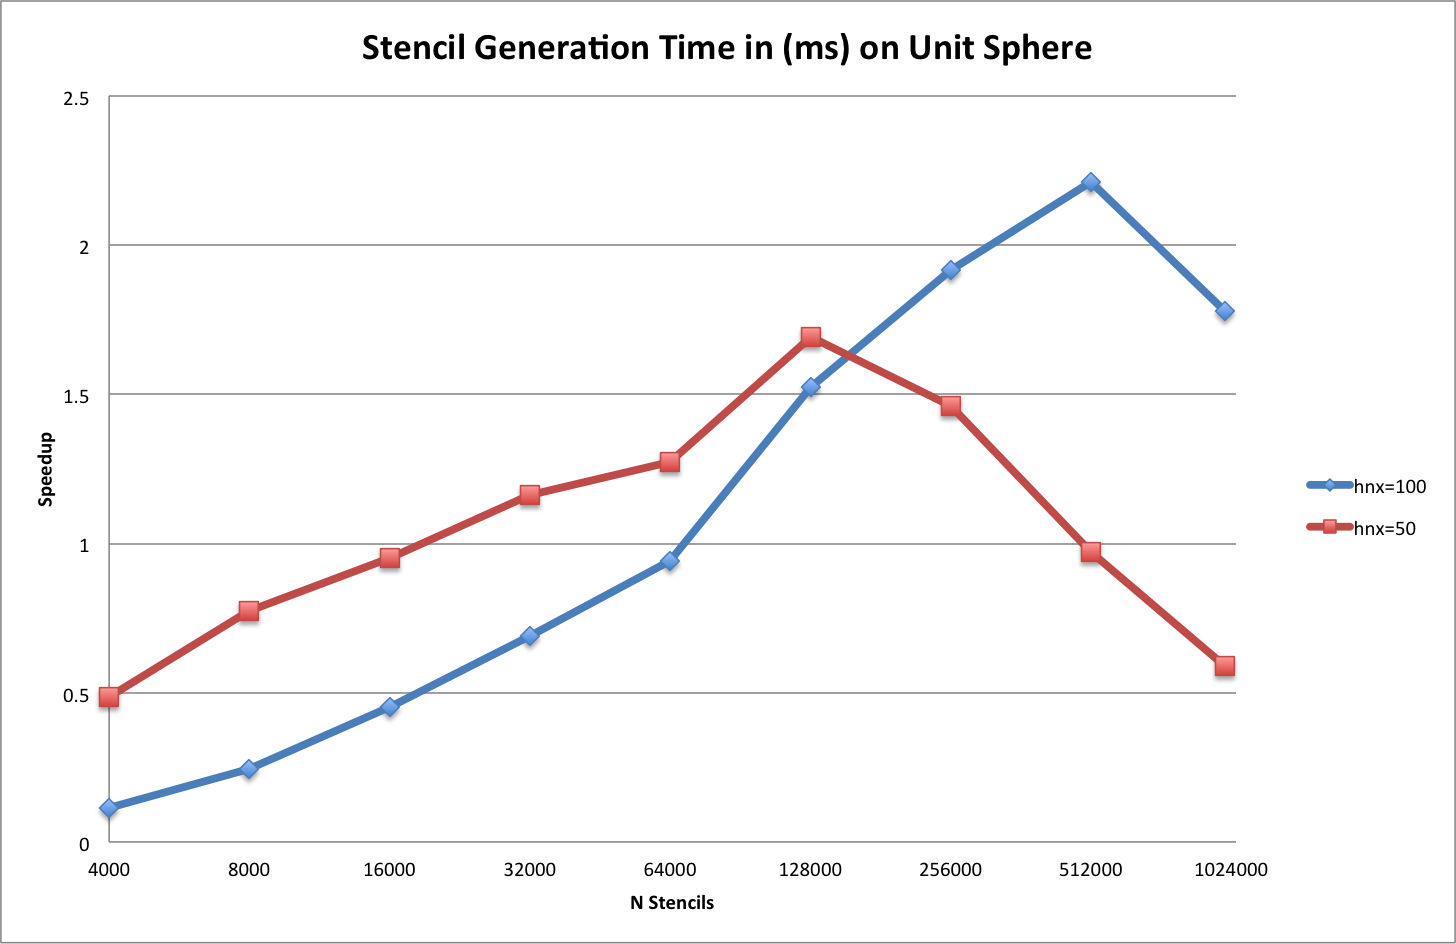
\includegraphics[width=6.5cm]{../figures/stencils/sphere_subsets_1m_stencil_gen_speedup.png}
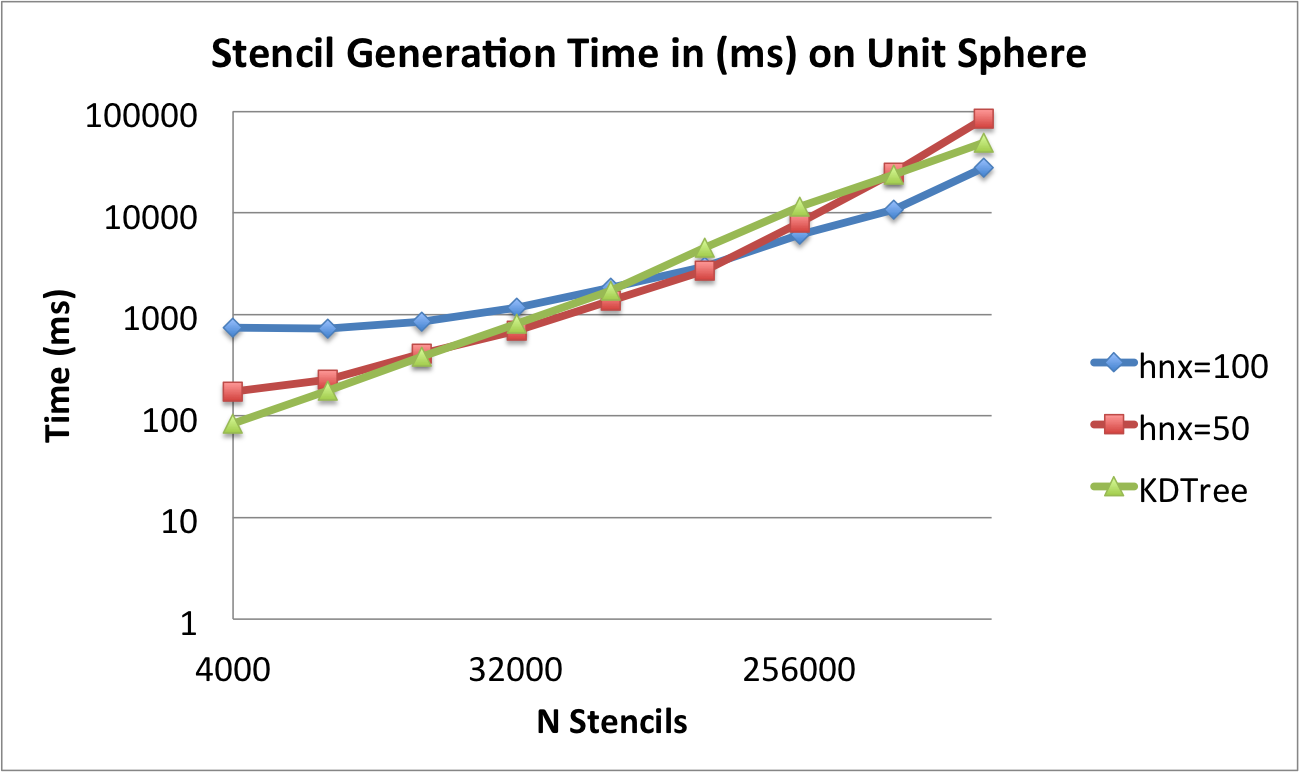
\includegraphics[width=6.5cm]{../figures/stencils/sphere_subsets_1m_stencil_gen_time.png}
\caption{Querying the $n=50$ nearest neighbors on a regular grid up to $N=160^3$ demonstrates the significant gains achieved by our spatially binned neighbor query. While KDTree queries grow as $O(N log N)$}
\label{fig:hash_results}
\end{figure}




\subsubsection{KDTree}
Most of the RBF community leverages the $k$-D tree, due to its low computational complexity for querying neighbors and its wide availability as standalone software in the public domain (e.g., matlab central has a few implementations for download, and the MATLAB Statistics Toolbox includes an efficient k-D Tree). 

The complexity of assembling he tree is

The Matlab central $k$-D Tree is MEX compiled and efficient. We integrated the standalone C++ code into our library.  

While the $k$-D Tree functions well for queries, its downfall is a large cost in preprocessing to build the tree. For moving nodes, such as in Lagrangian schemes, this cost is prohibitively high. In an attempt to reduce the cost, lagrangian schemes introduced approximate nearest neighbor queries based on 


\subsubsection{Hashing}

Approximate nearest neighbors will be nearly balanced. 
We observe that RBF-FD functions as well on stencils of true nearest neighbors as it does on approximate nearest neighbors.

Consider Figure~\ref{fig:ann_stencil} in which an Approximate Nearest Neighbor stencil is constructed. For this stencil, all but one of the nearest neighboring nodes are chosen. 

\begin{figure}
\centering
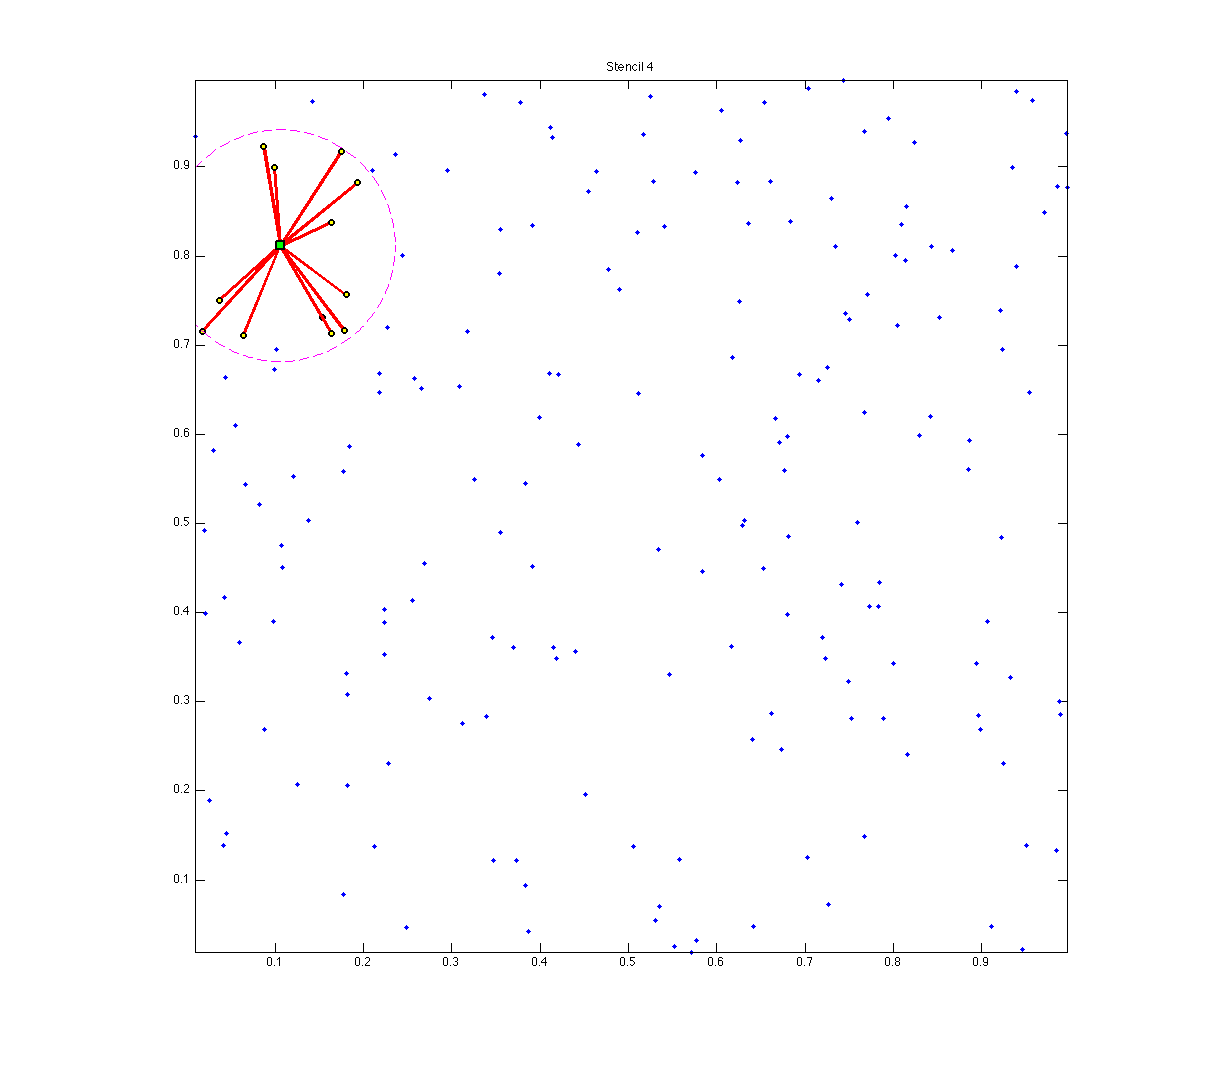
\includegraphics[width=0.6\textwidth]{rbffd_methods_content/neighbors/neighbor_incorrect.png}
\caption{Example of an Approximate Nearest Neighbor (ANN) stencil, with all but one of the true nearest neighbors included in the stencil. }
\label{fig:ann_stencil}
\end{figure}



Hashing, shown in Figure~\ref{fig:hashing_example} overlays a regular grid. This is equivalent to an axis aligned bounding box AABB, with refinement. In other words, we form a quad-tree in 2D, an octree in 3D. The neighbor query starts with the cell in which $x_c$ resides. Since we use an axis aligned bounding box, this cell index is easily calculated given the coordinate and number of subdivisions in each dimension. Once the cell index is resolved, the stencil is populated by taking the $n$ nearest neighbors from within the current cell. If the cell does not contain sufficient number of nodes to fill the stencil, the search for neighbors expands to include the cells immediately adjoining the center cell, taking only the nearest nodes in the provided cells. The search continues to expand outward in a rasterized circle/sphere until $n$ is satisifed. This search is considered approximate because it can happen that a true nearest neighbor would lie in a cell that is is not included in the rasterized circle, and other nodes are substituted from the far reaches of the discretized grid.

%TODO: cite lagrangian sph knn
The complexity of the method is still higher than the more efficient implementations used by Lagrangian methods, but as demonstrated in Figure~\ref{sten_methods_compare} the savings are significant. Generating stencils for RBF-FD is a preprocessing cost, so we do not dedicate an excessive amount of attention to this algorithm. However, a few ideas that would improve: hilbert ordering, choose AABB resolution based on $N$ not user parameters, faster sorting, GPU implementation


To demonstrate the savings in choice of stencil generation method, we provide Figure~\ref{fig:sten_methods_compare}. 
 

The impact of our neighbor query also extends influence on the structure of the RBF-FD DMs.
has is to To quantify the sparsity of a Differentiation Matrix we consider the ratio of non-zeros ($N*n$) to total elements in the matrix ($N^2$). For example, a problem of size $N = 10,000$ with stencil size $n=31$ has a ratio of $0.0031$ and is $99.69\%$ empty. 

Querying neighbors requires searching at least the immediate cell one layer of neighbors. by including one extra layer we ensure that small stencils near the border of the immediate cell can pick up neighbors in adjacent cells.


%TODO: sparsity
%TODO: Node ordering
%TODO: show blocks for boundary conditions (annulus)



\begin{figure}
\centering
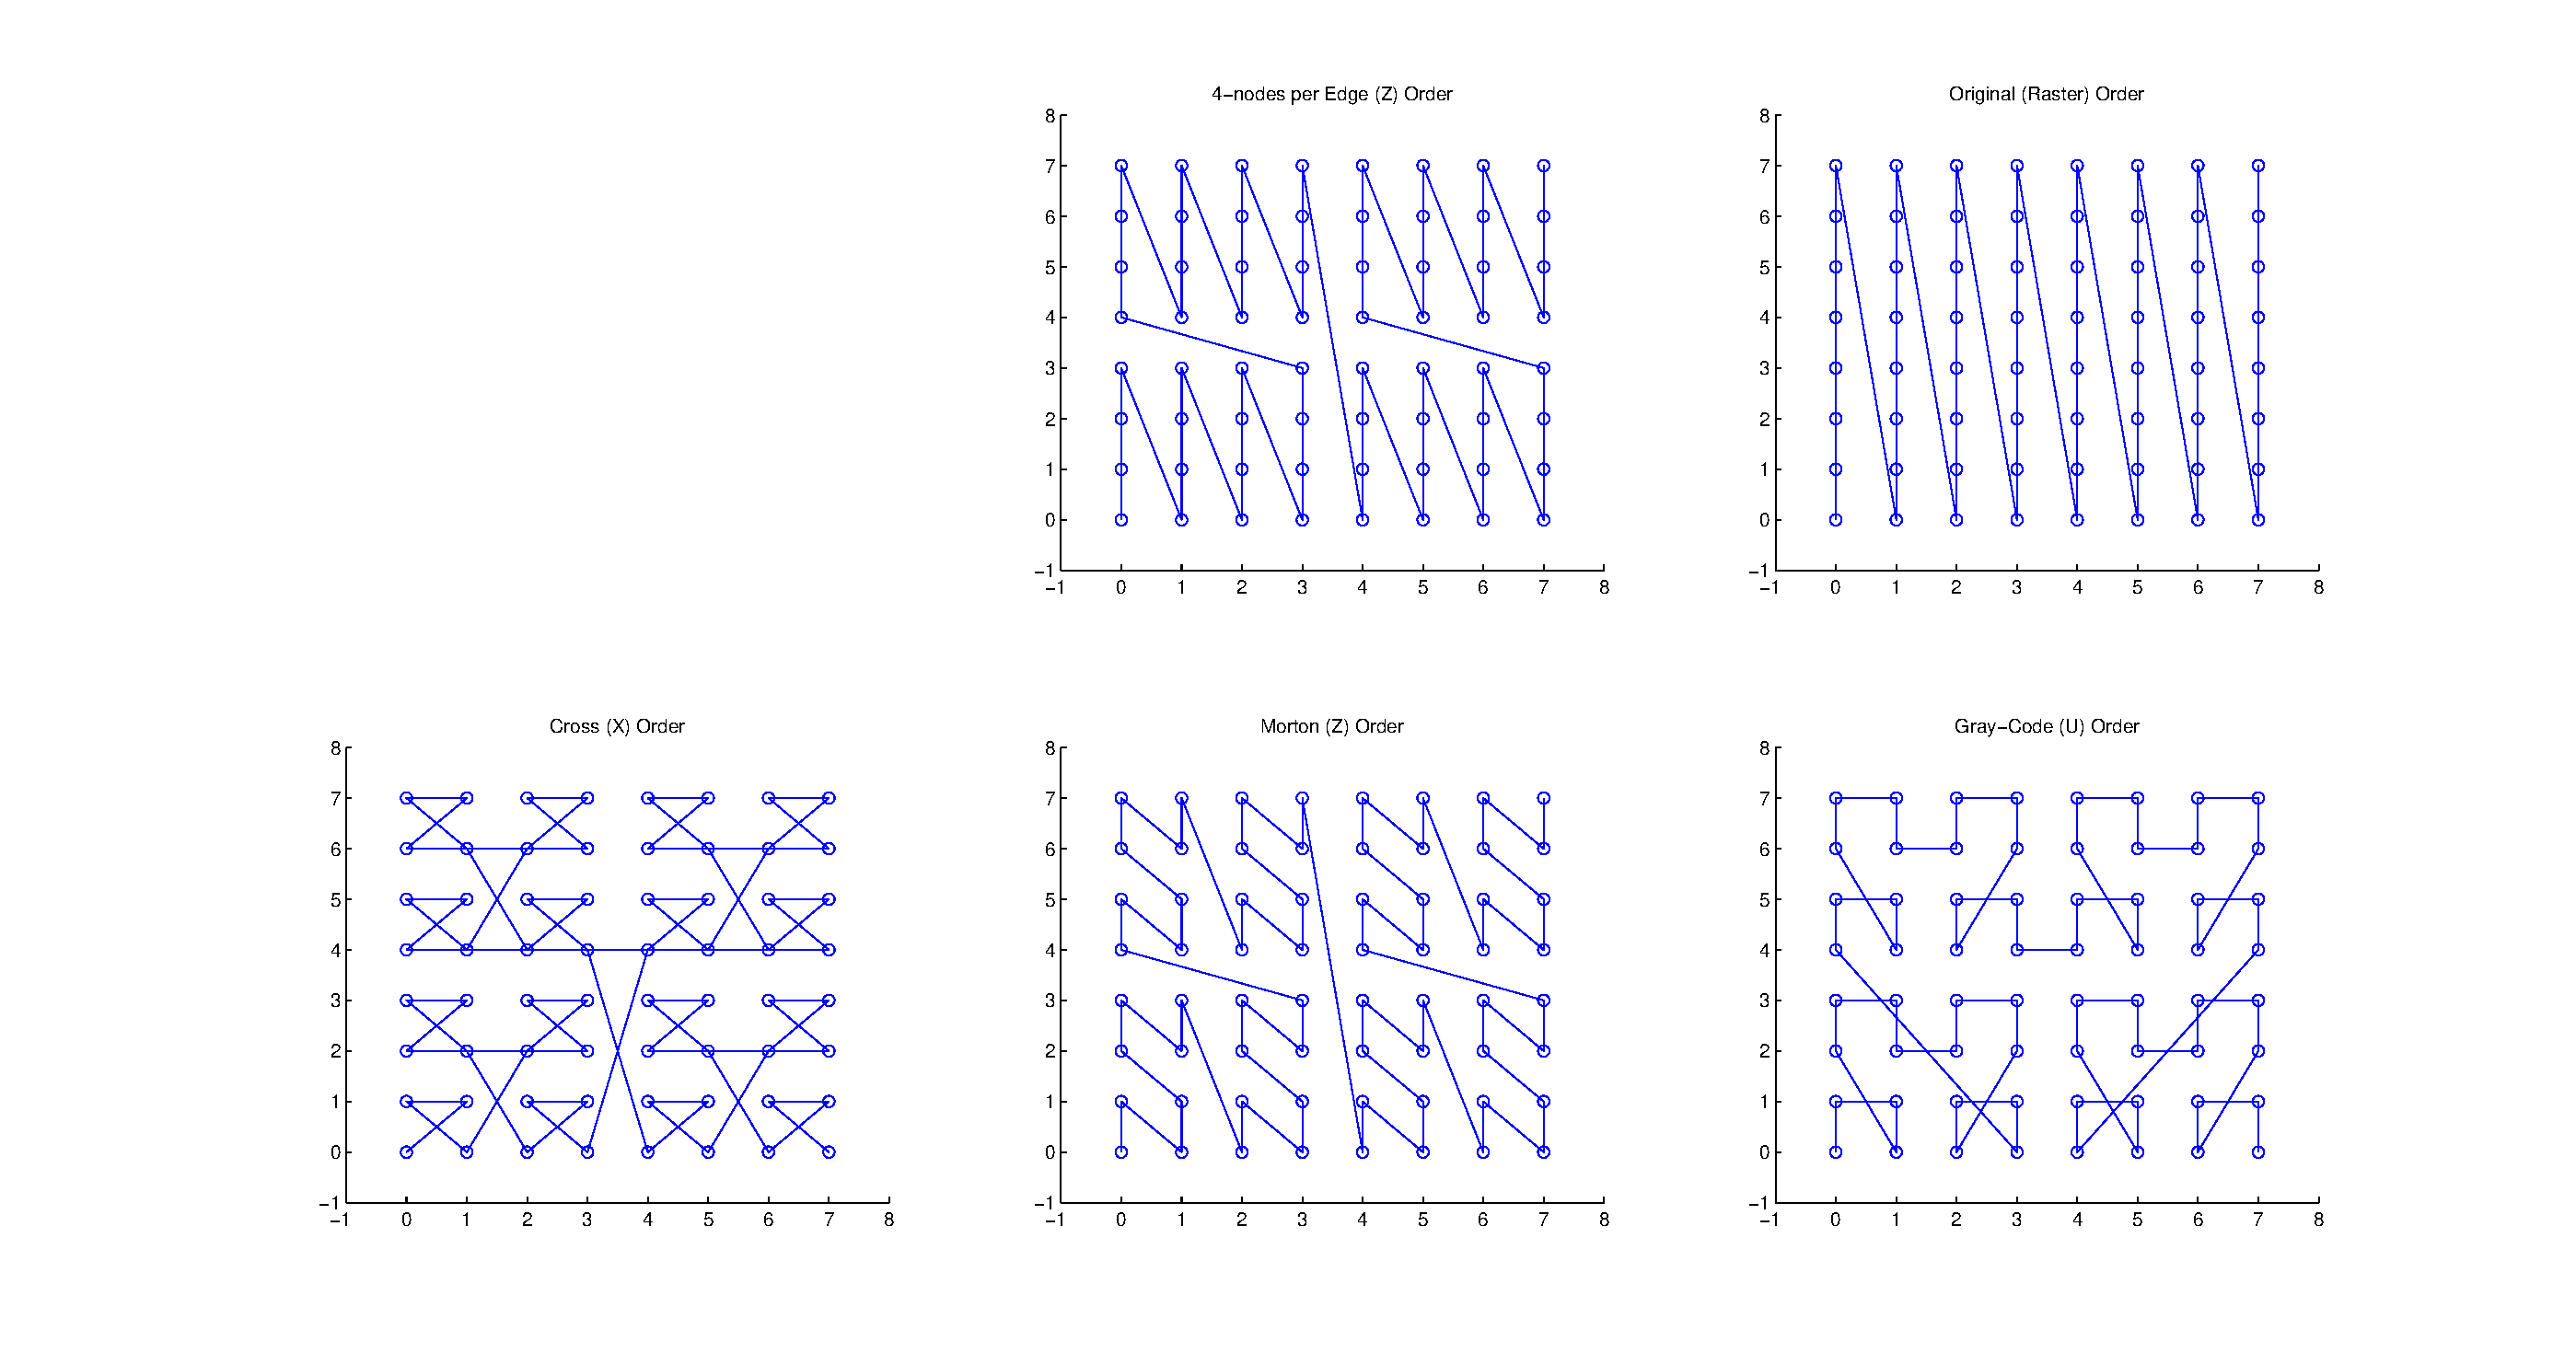
\includegraphics[width=0.65\textwidth]{rbffd_methods_content/hashing/node_orderings.eps} \\
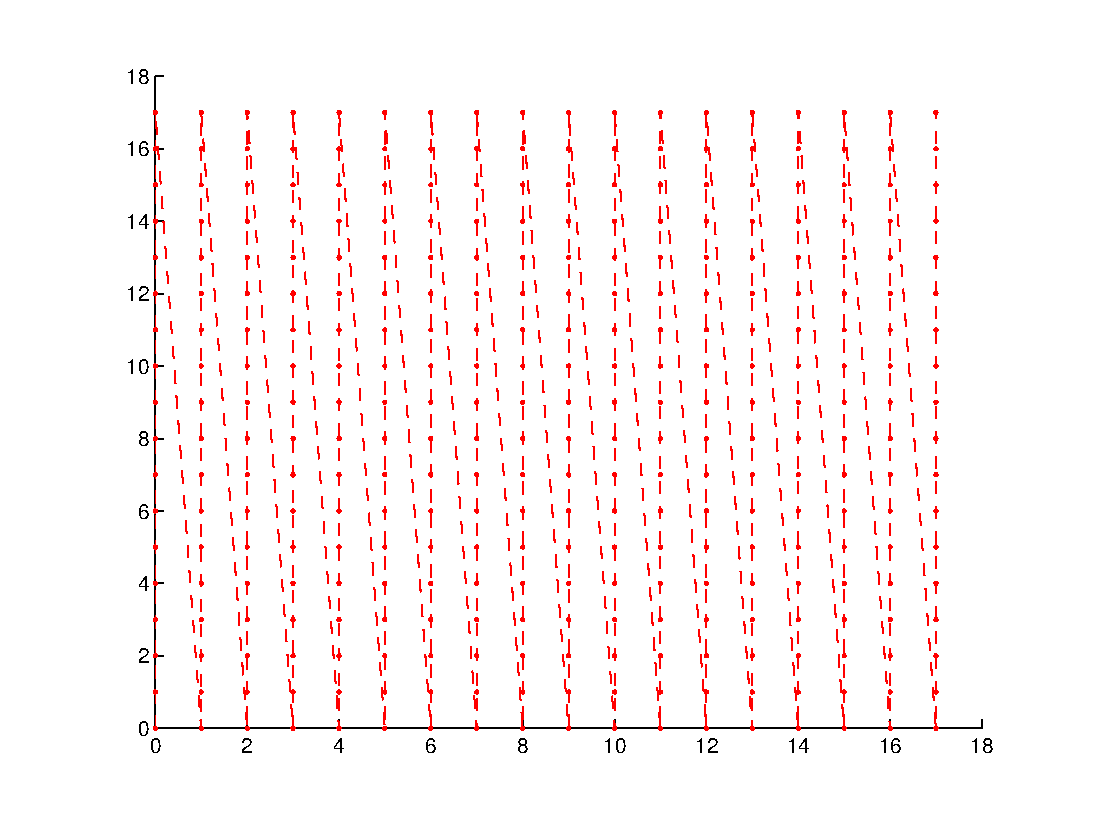
\includegraphics[width=0.45\textwidth]{rbffd_methods_content/hashing/originalorder_regulargrid.eps} \\
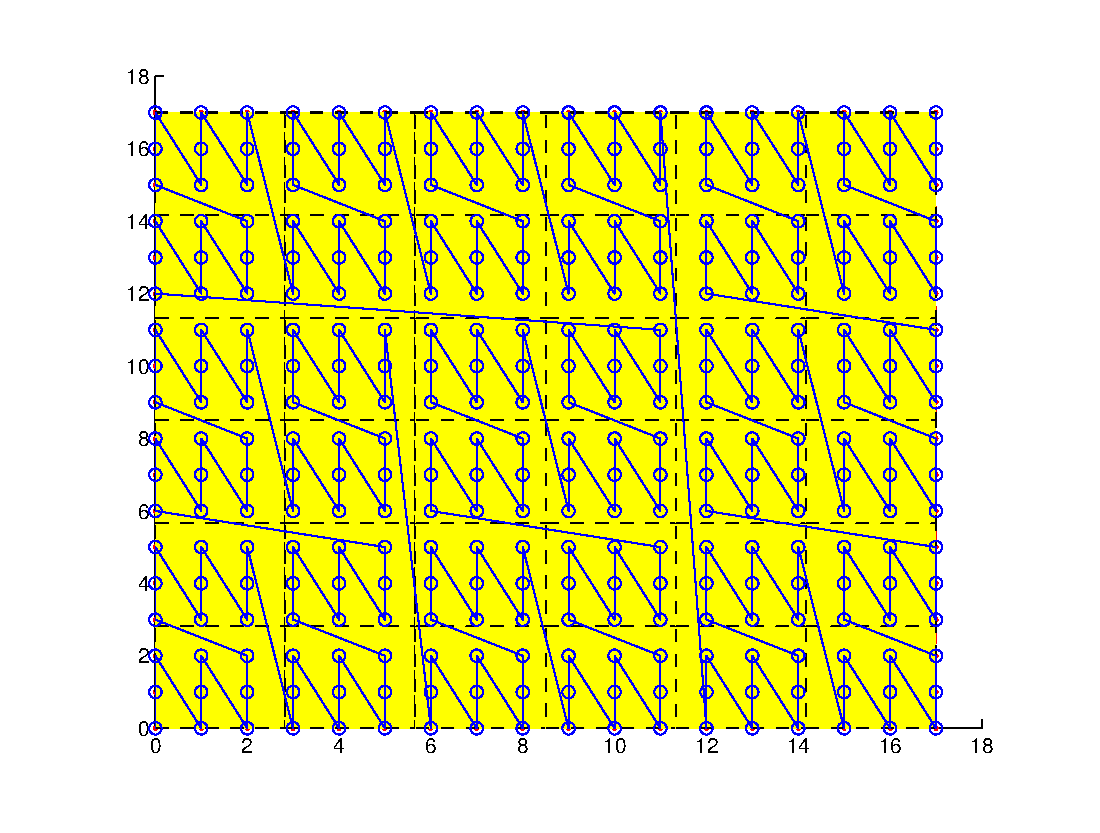
\includegraphics[width=0.45\textwidth]{rbffd_methods_content/hashing/overlay_regulargrid.eps} 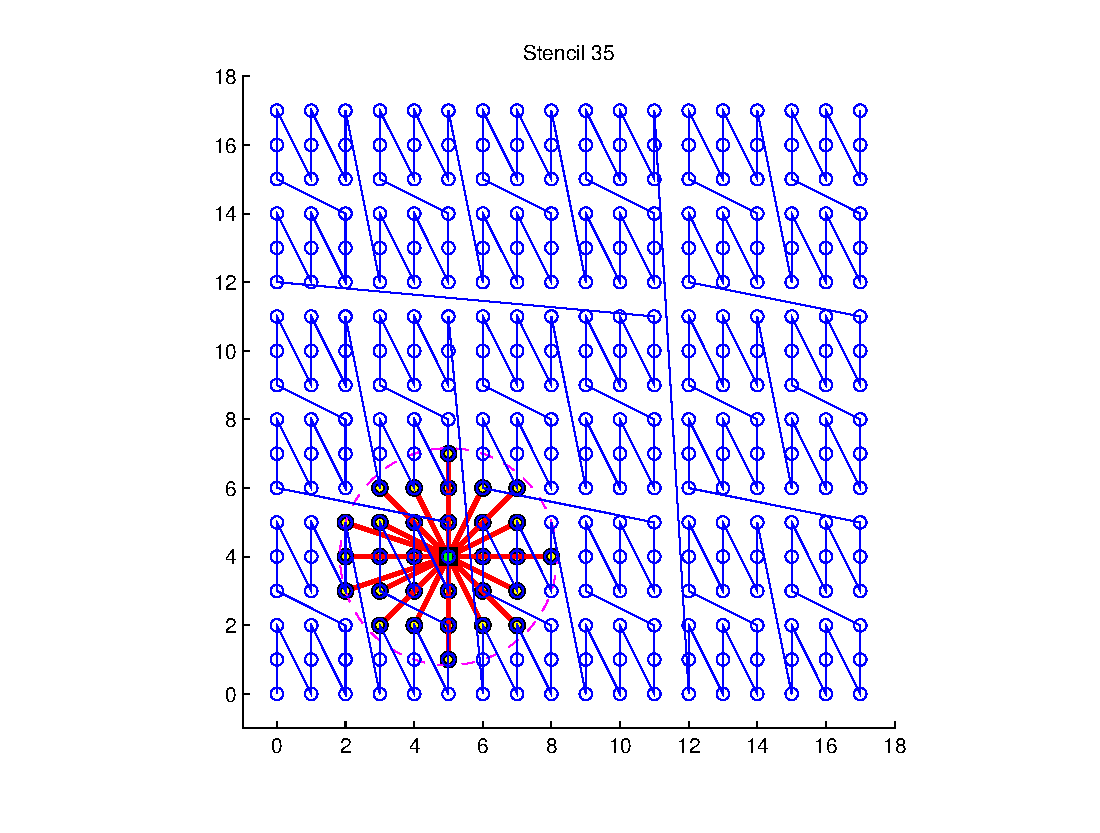
\includegraphics[width=0.45\textwidth]{rbffd_methods_content/hashing/stencil_regulargrid.eps} \\
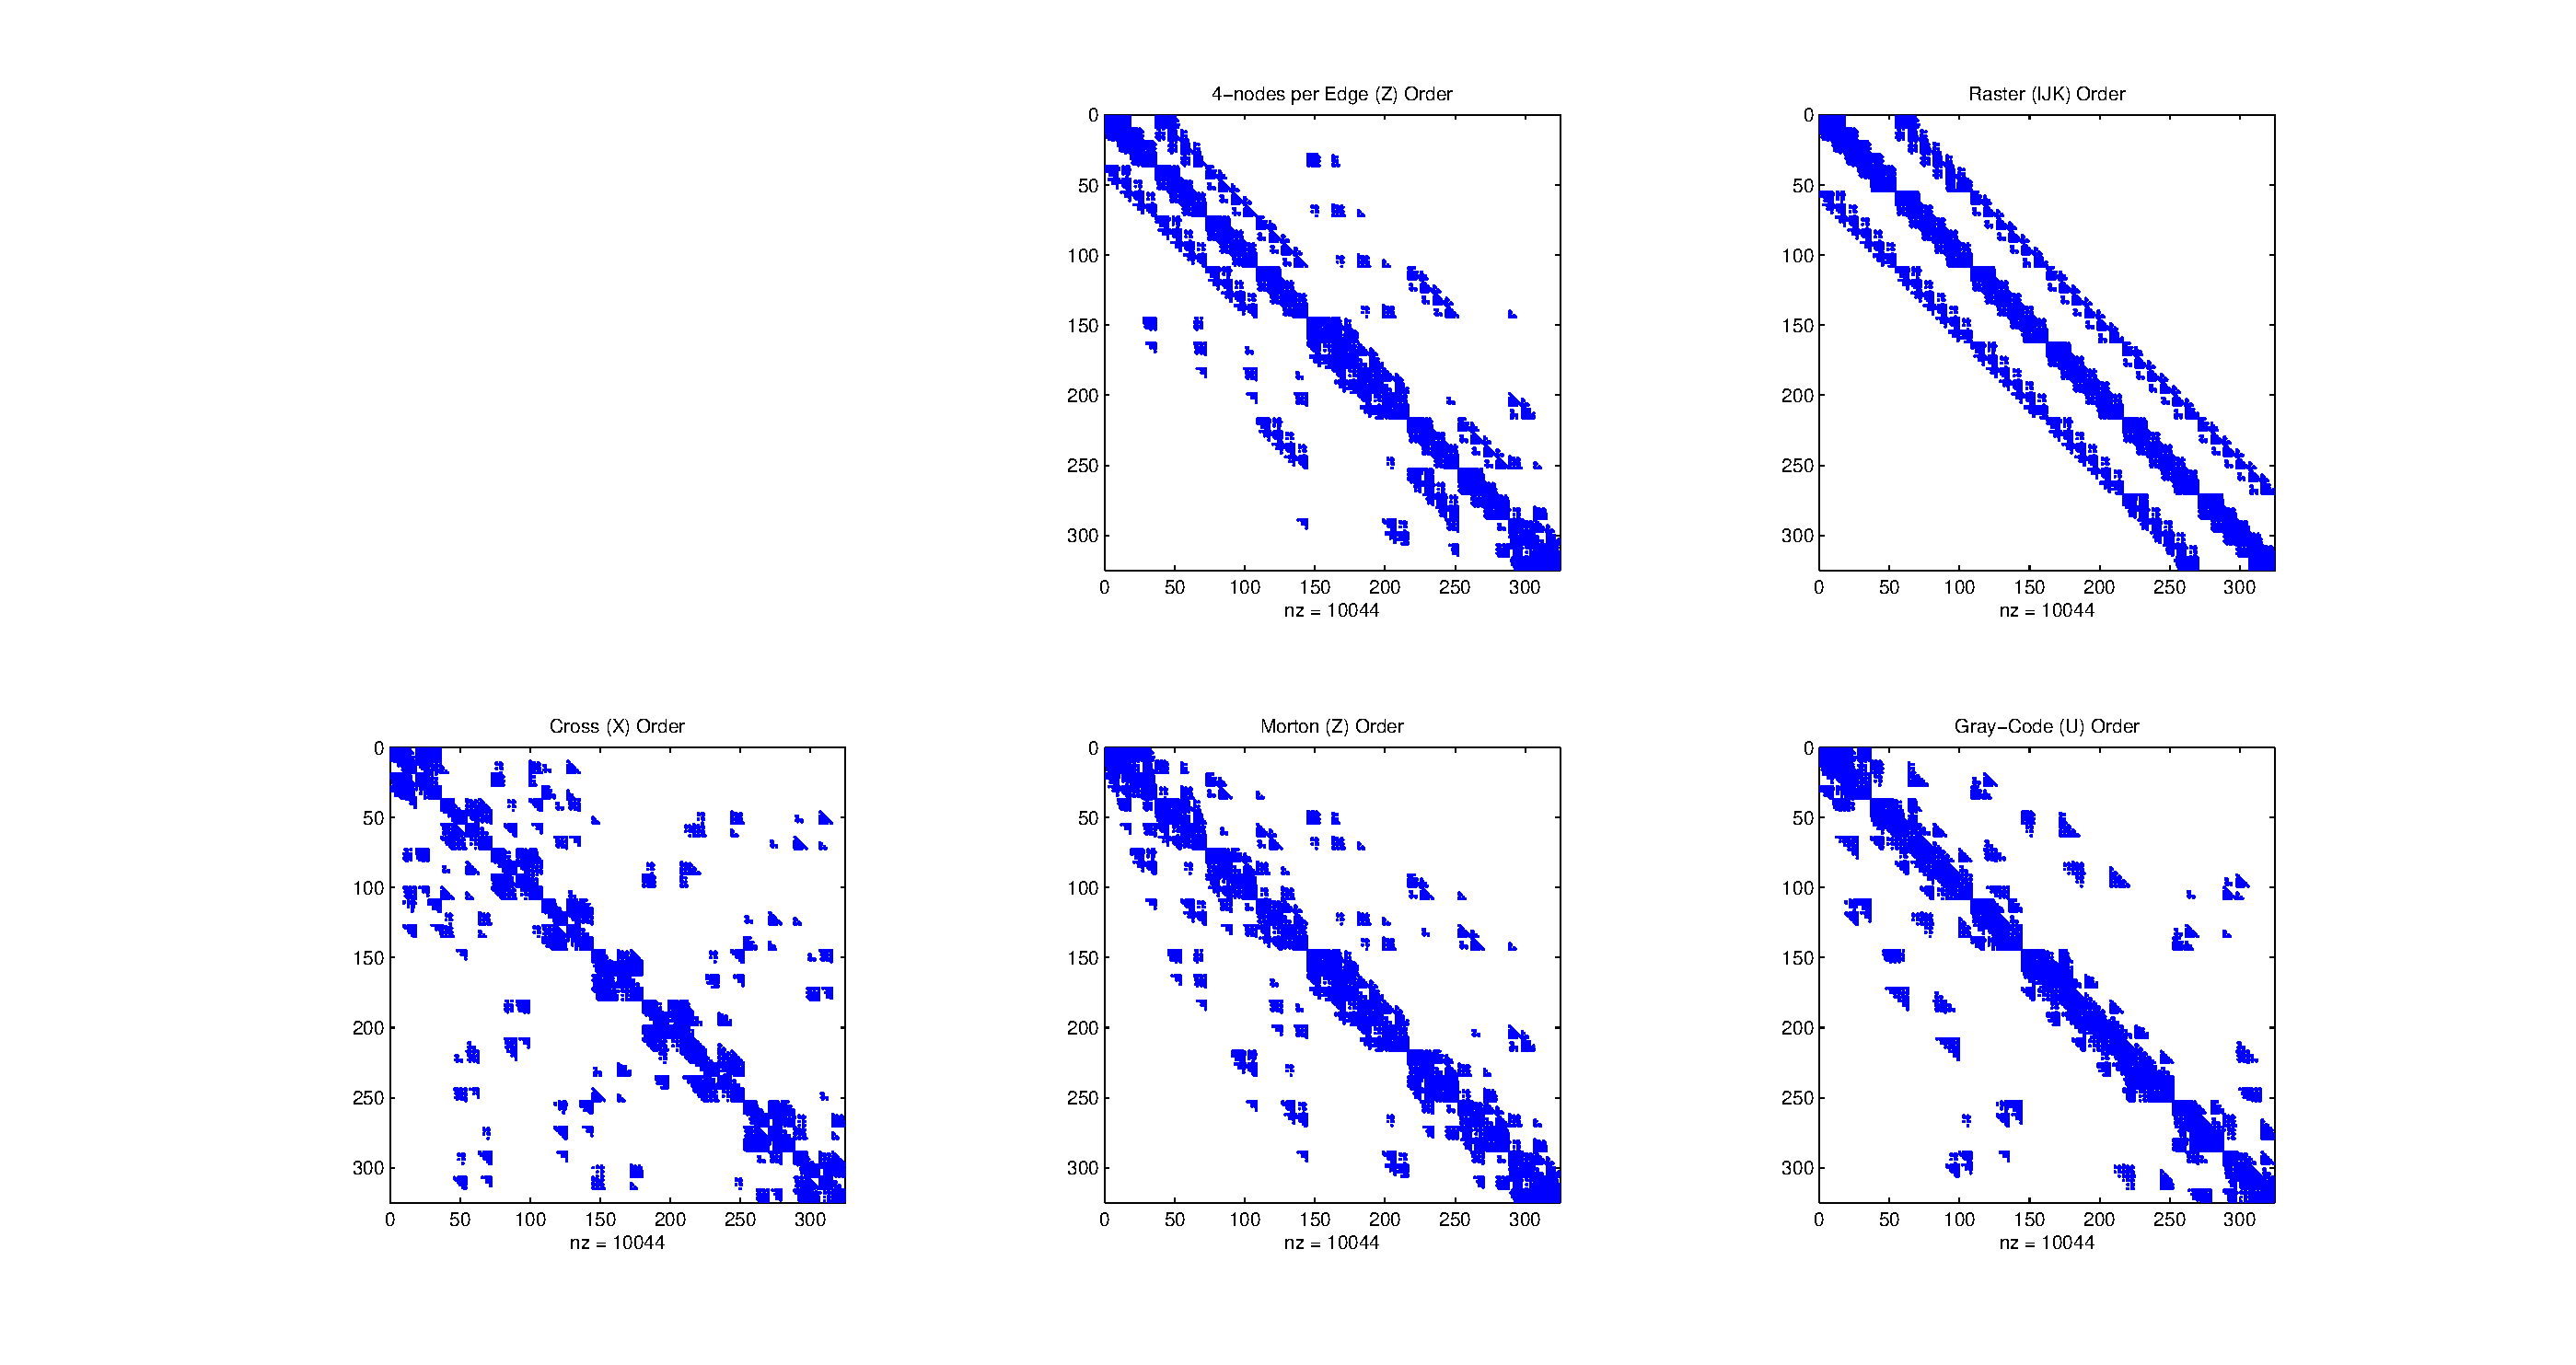
\includegraphics[width=0.65\textwidth]{rbffd_methods_content/hashing/spy_regulargrid.eps} 
\caption{In order: a) node ordering test cases; b) original ordering of regular grid (raster); c) coarse grid overlay for hash functions ($hnx = 6$); d) example stencil ($n=31$) spanning multiple Z's; e) spy of DM after orderings. }
\label{fig:orderings}
\end{figure}

The KDTree implementation used in this work is from 

Original data showed our algorithm as wildly successful against a version  


%TODO: get the compareKDTreeLSH.m output; this was for my C++ code and compared queries on 
%\begin{figure}
%\centering
%\includegraphics[width=0.65\textwidth]{rbffd_methods_content/hashing/
%\end{figure}



%TODO: \cite{Indyk "Algorithms for Nearest Neighbor Search"} for reference on quad vs kd vs lsh
%TODO: \cite{ChenChang "Neighbor-Finding Based on Space-Filling Curves"} 
%TODO: \cite{Stocco and Schrack "On Spatial Orders and Location Codes"}


Obviously, the ideal case for bandwidth is when all rows contain the $\frac{n}{2}$ nodes corresponding to solution value to either side of $u_j$. In 1-D this corresponds to every node containing the $\frac{n}{2}$ nodes to the left and right of $x_j$. In 2-D this is only possible if the nodes in the domain are properly indexed such that stencils contain the proper set of neighbors---a stringent requirement that will 




\subsection{On Choosing the Right $\epsilon$} 
% TODO: expand missing content



%First, the method is not infallible; it faces similar conditioning issues as global/compact RBF method in that the success of the method depends on the choice of support parameter, $\epsilon$. Second, proper choice of $\epsilon$ varies based on the underlying node distribution, as well as the generated stencils. Third, the complexity of the method is low, but there are a few 

If solving for the weights directly (i.e., inverting Equation~\ref{eq:rbffd_weight_system}), one must carefully choose $\epsilon$ to prevent ill-conditioning. Numerous attempts exist in literature to provide ``good" functions for $\epsilon$ based on node spacing, $h$, stencil size $n$, etc. In general, the values provided are particular to the specific problem and/or grid under consideration. No fool-proof method exists to select the support parameters, so the prospect of hassle-free application of the RBF-FD method is still out of reach. 

Modern algorithms introduced in the last couple years provide methods for acquiring weights. Contour-Pad\'{e}, RBF-QR, and RBF-GA are all options for weights corresponding to the $\epsilon \rightarrow 0$. These methods appear to resolve many issues including conditioning of implicit systems for more accurate solutions \cite{Davydov2011}  \cite{Fornberg2013} 

In this work, we have attempted a variety of scalings on $\epsilon$. We forego discussion of these attempts since they are outside our current scope of investigation. In the end, we find that the most effective method for choosing $\epsilon$ was to adopt the approach introduced in \cite{FlyerLehto11}, wherein $\epsilon$ is expressed as a function of the number of nodes $N$ and desired mean condition number, $\bar{\kappa}_A$. 

%TODO: what papers provide epsilon choice? based on grid? based on node density? proportional to what?
%TODO: what is the algorithm to choose epsilon?
%TODO: what examples are provided? 
%TODO: does the choice of c1 and c2 depend on the problem? 
%TODO: what level coarse grid is necessary to get contours? 
%TODO: what other epsilon tests? why not uniform epsilon? why not variable epsilon? 

%TODO: add references and descriptions. 
The optimal $\epsilon$ for general node distributions is out of the scope of this research and not necessary for our purposes. For now we assume that nodes are more or less regularly distributed, either via some algorithm such as Lloyd's method to create Centroidal Voronoi Tessellations, repelling springs (distmesh), minimum energy or minimum determinant, or some other algorithm. Except in cases where convergence on PDE solutions can not be attained via RBF-FD, we find that a direct solve for RBF-FD weights is sufficient. To a certain extent, this work considers parallelization of the method so it does not matter if our weights are precise or not. 


We adopt similar appraoch as \cite{FlyerLehto11} by choosing the same epsilon values specified in Table~\ref{tbl:vortex_hv_params}. 

I also produced a Matlab script to generate the contours for any stencil size and produced the following figures. 

\begin{figure}[htbp]
\centering
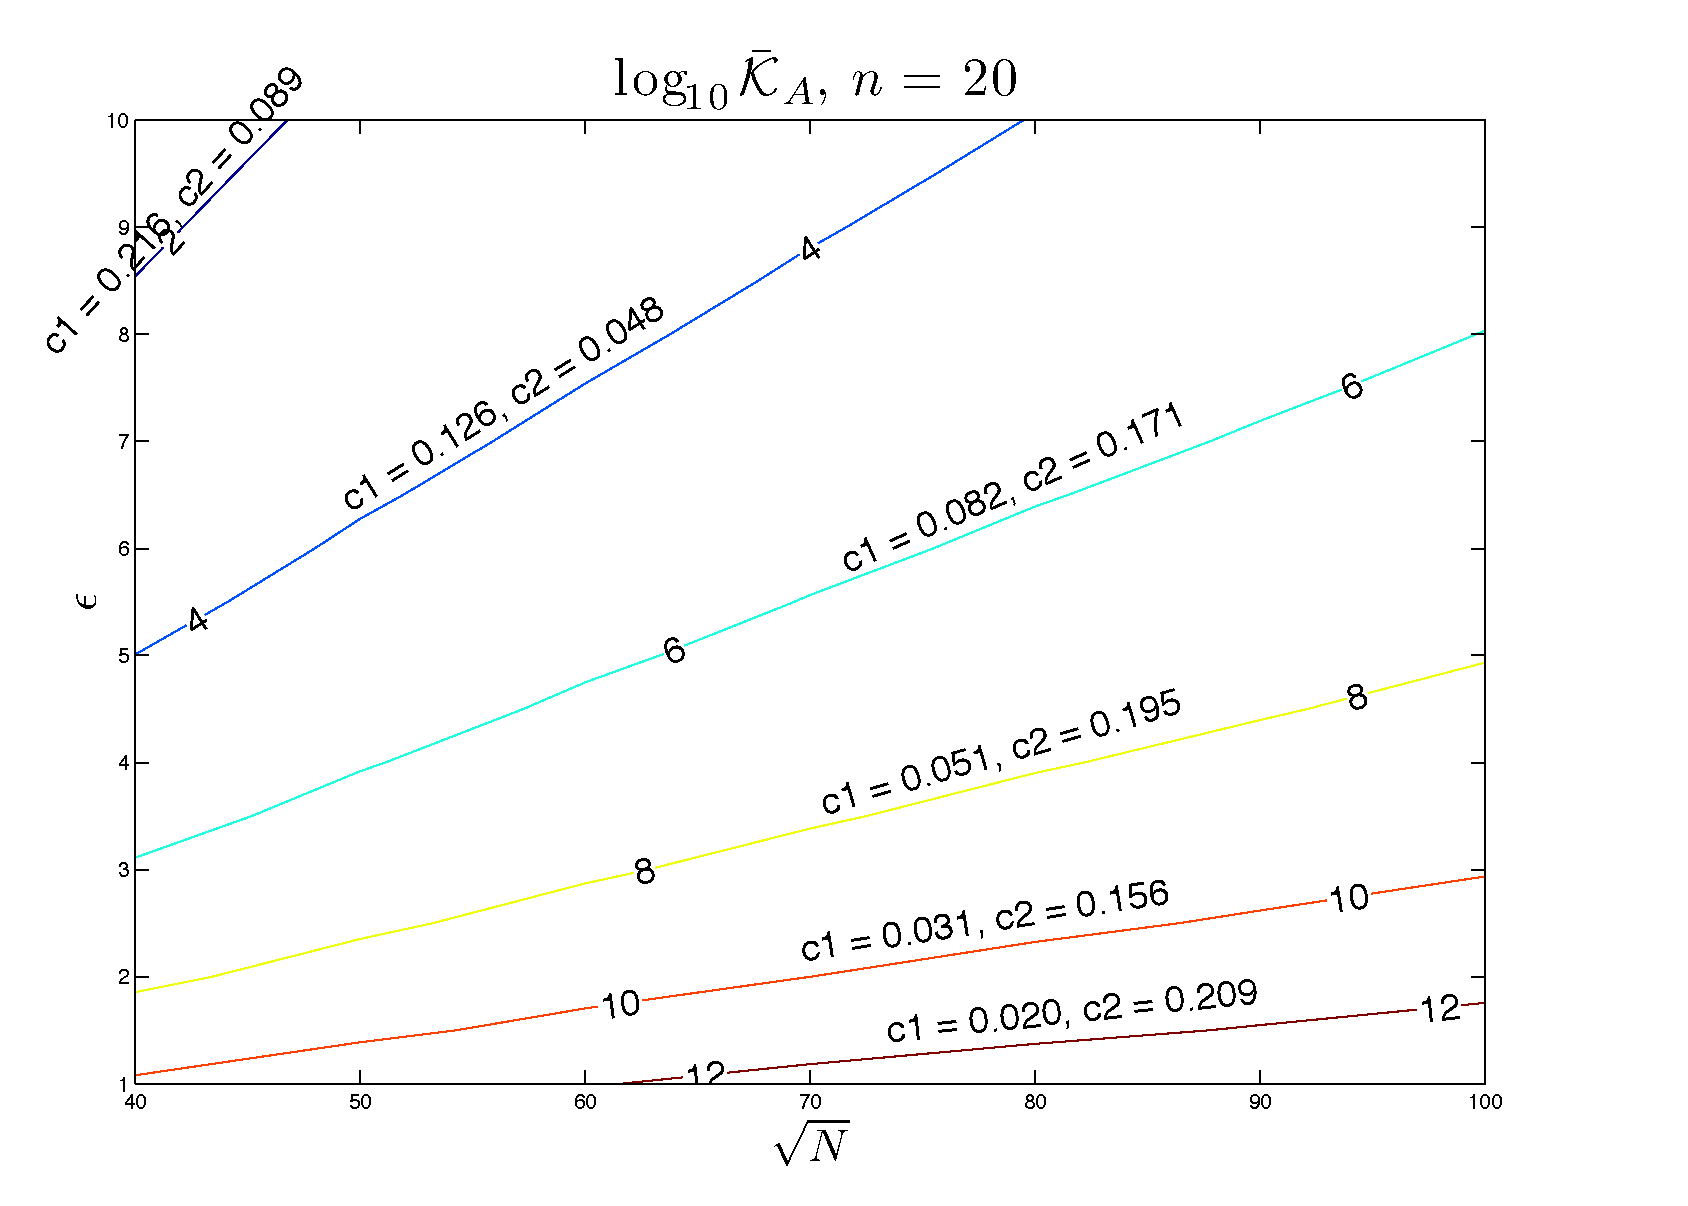
\includegraphics[width=0.45\textwidth]{../figures/chapter2/epsilon_contours/labeled_contour_n20.pdf}
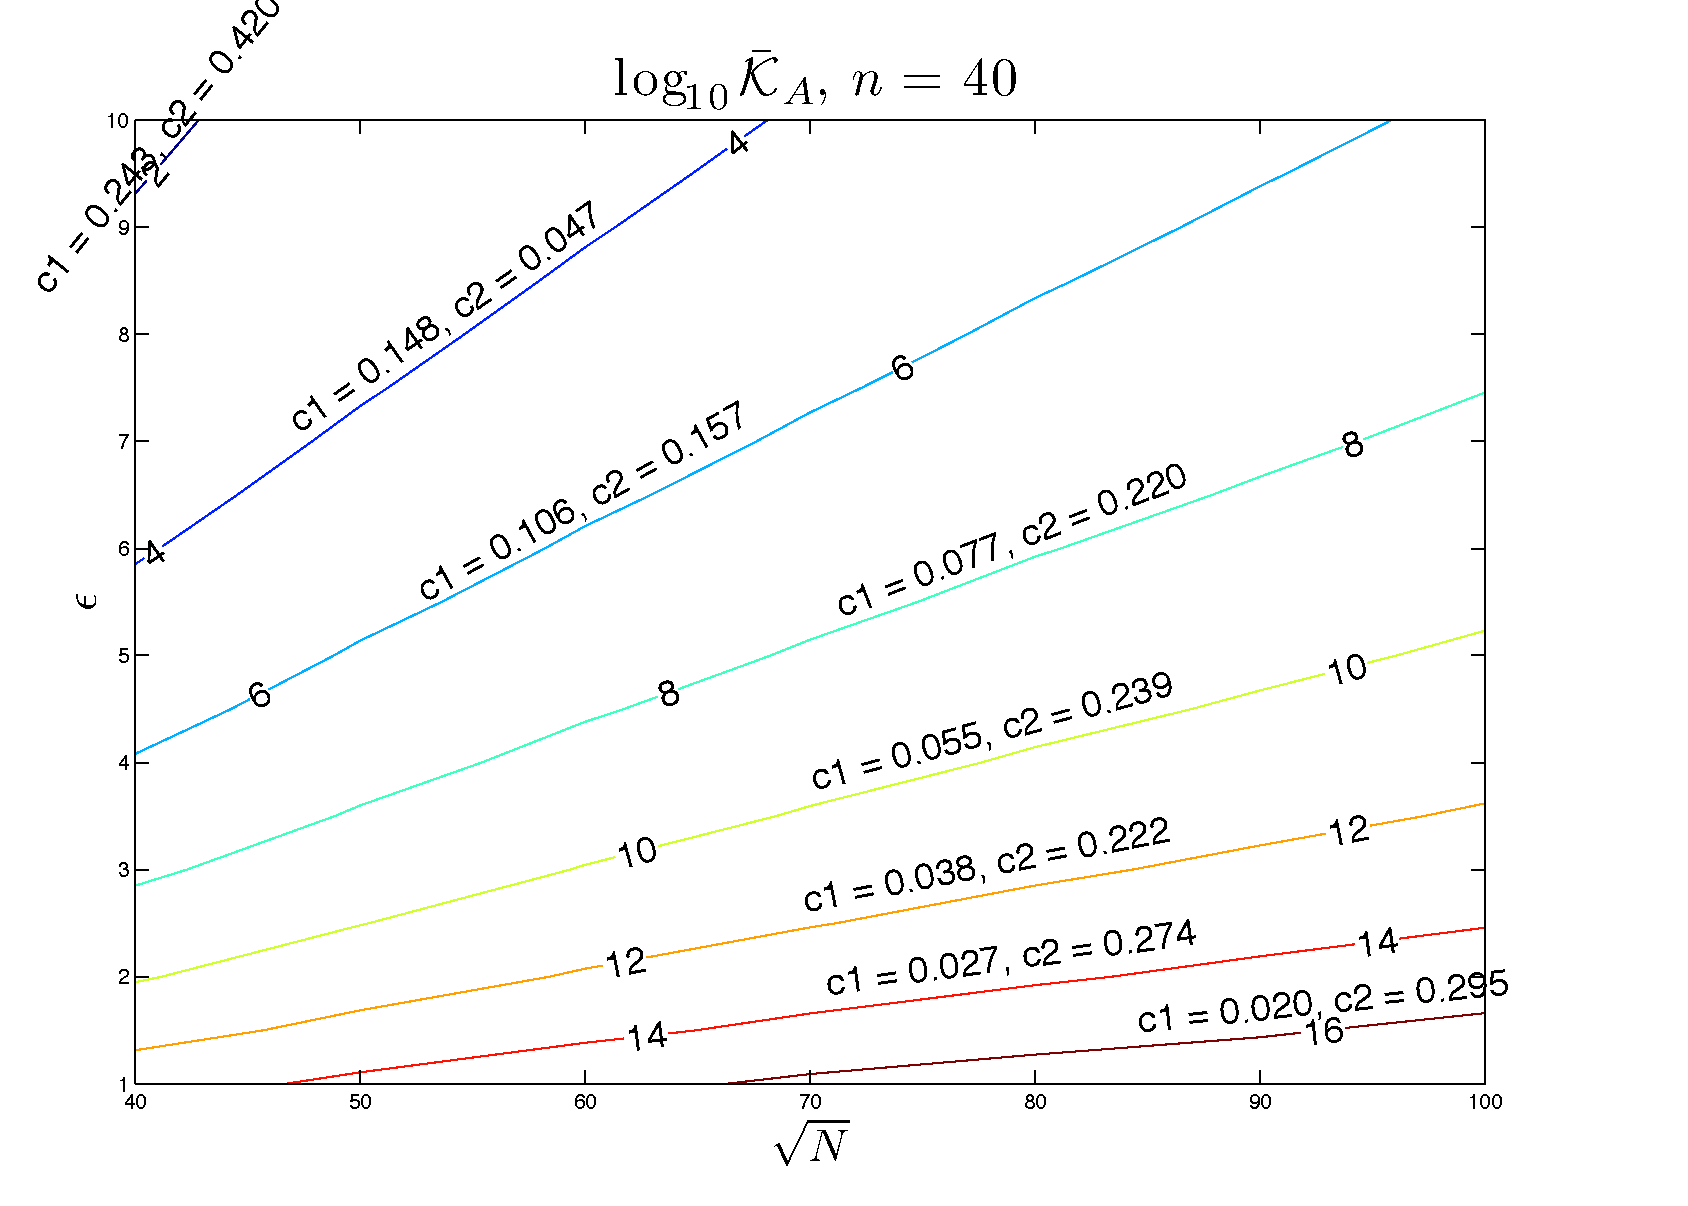
\includegraphics[width=0.45\textwidth]{../figures/chapter2/epsilon_contours/labeled_contour_n40.pdf}
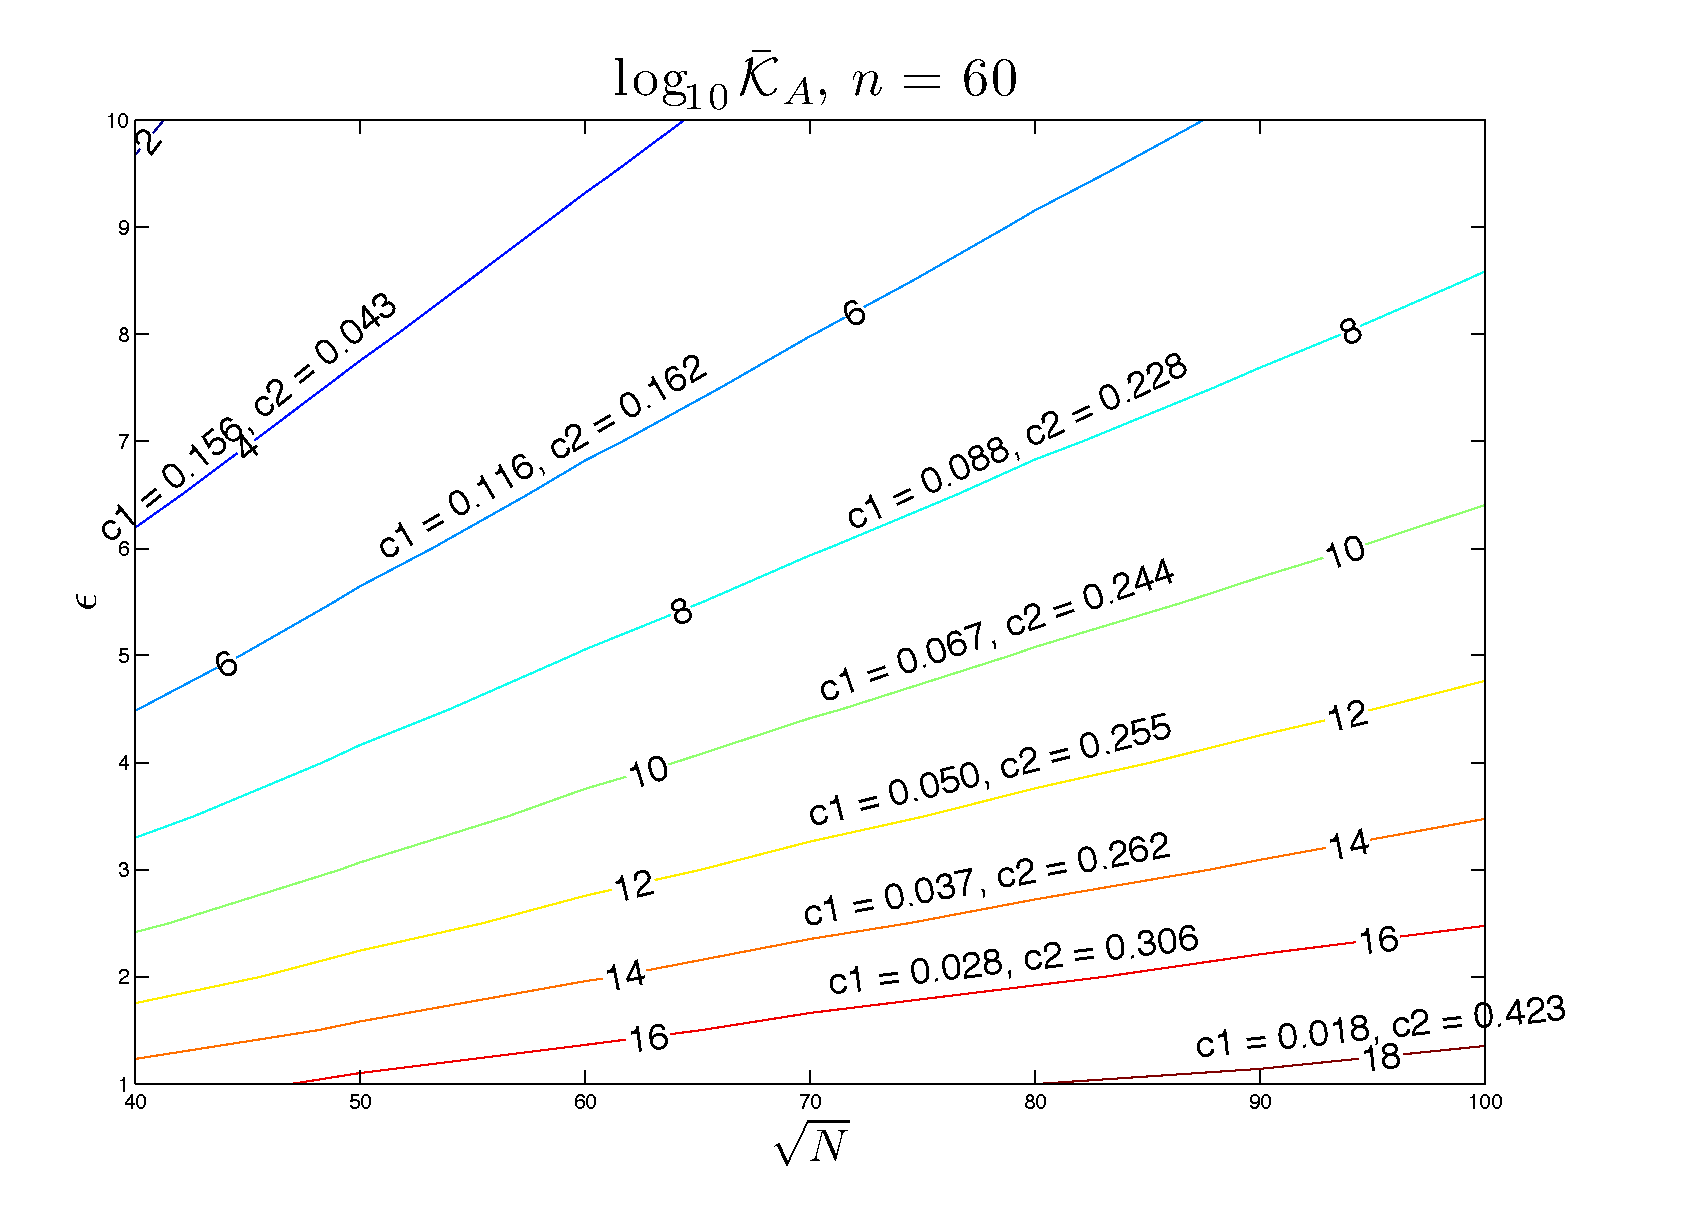
\includegraphics[width=0.45\textwidth]{../figures/chapter2/epsilon_contours/labeled_contour_n60.pdf}
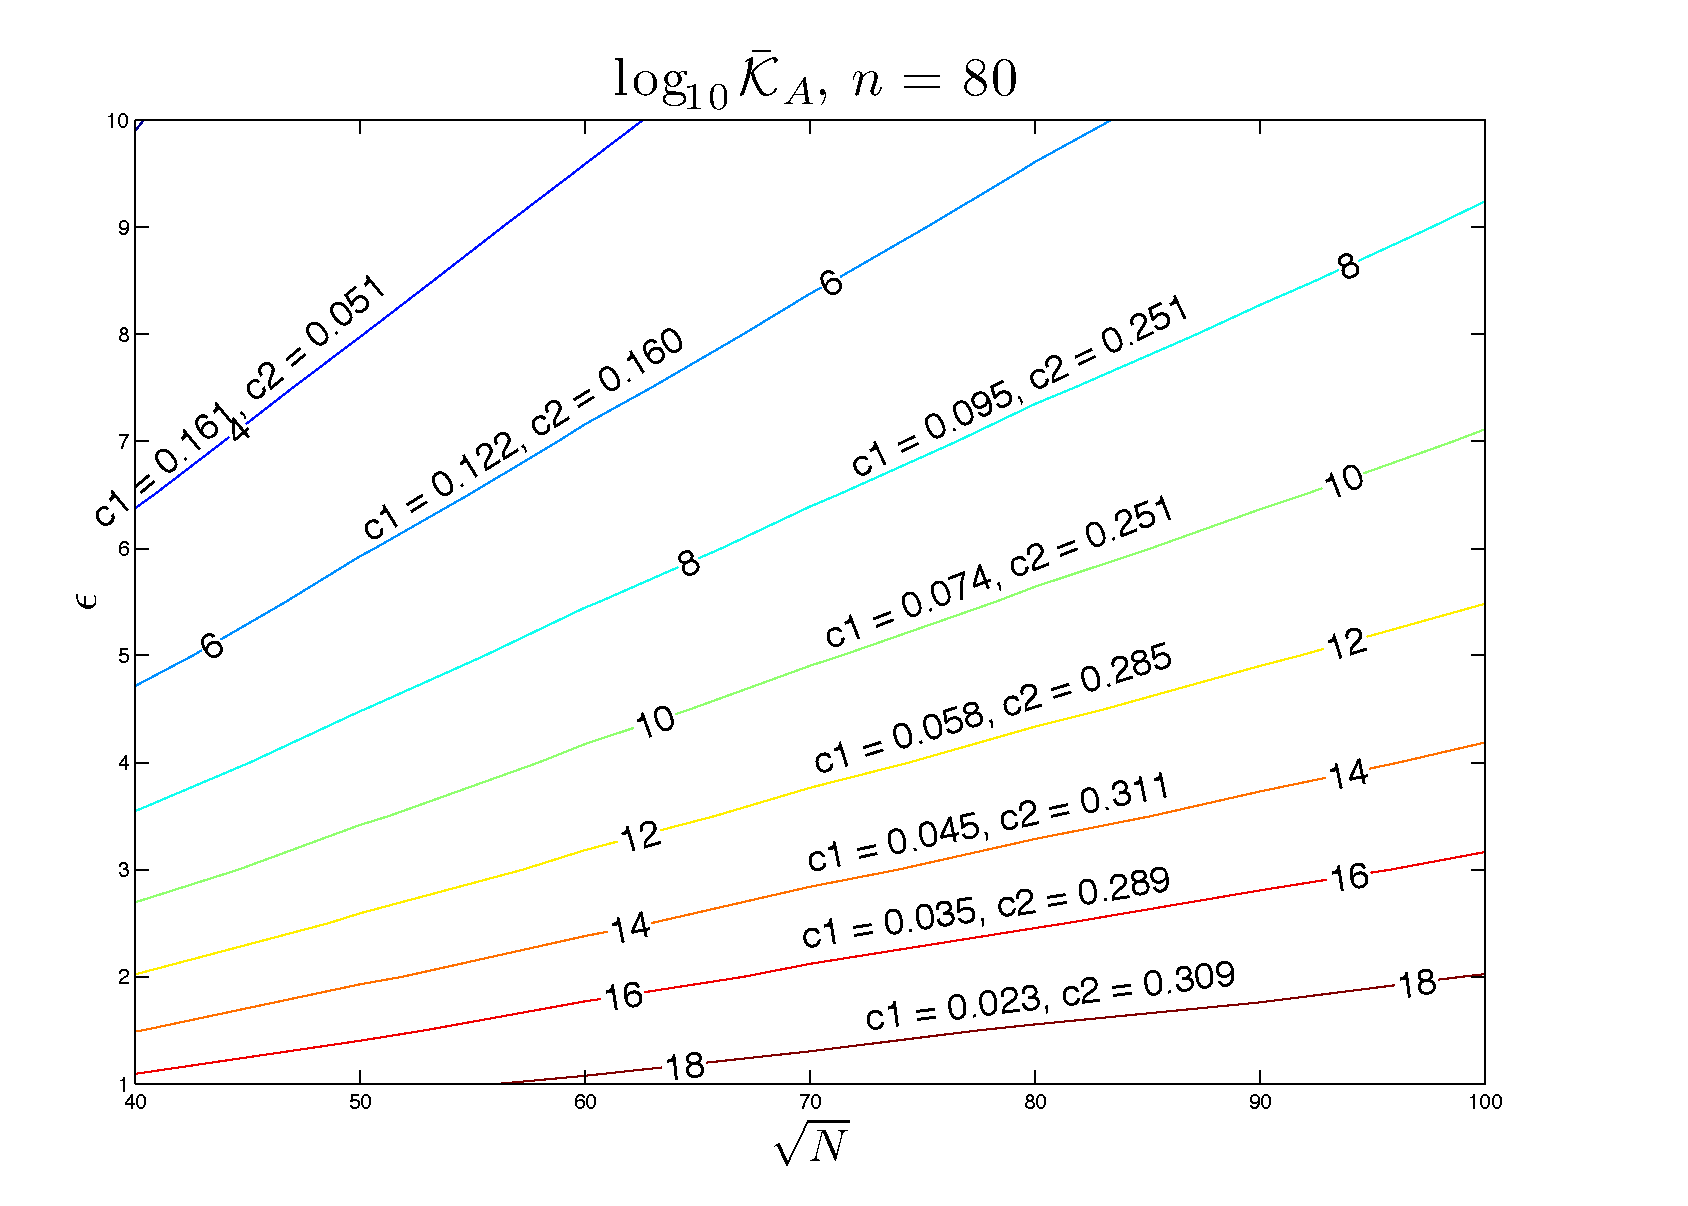
\includegraphics[width=0.45\textwidth]{../figures/chapter2/epsilon_contours/labeled_contour_n80.pdf}
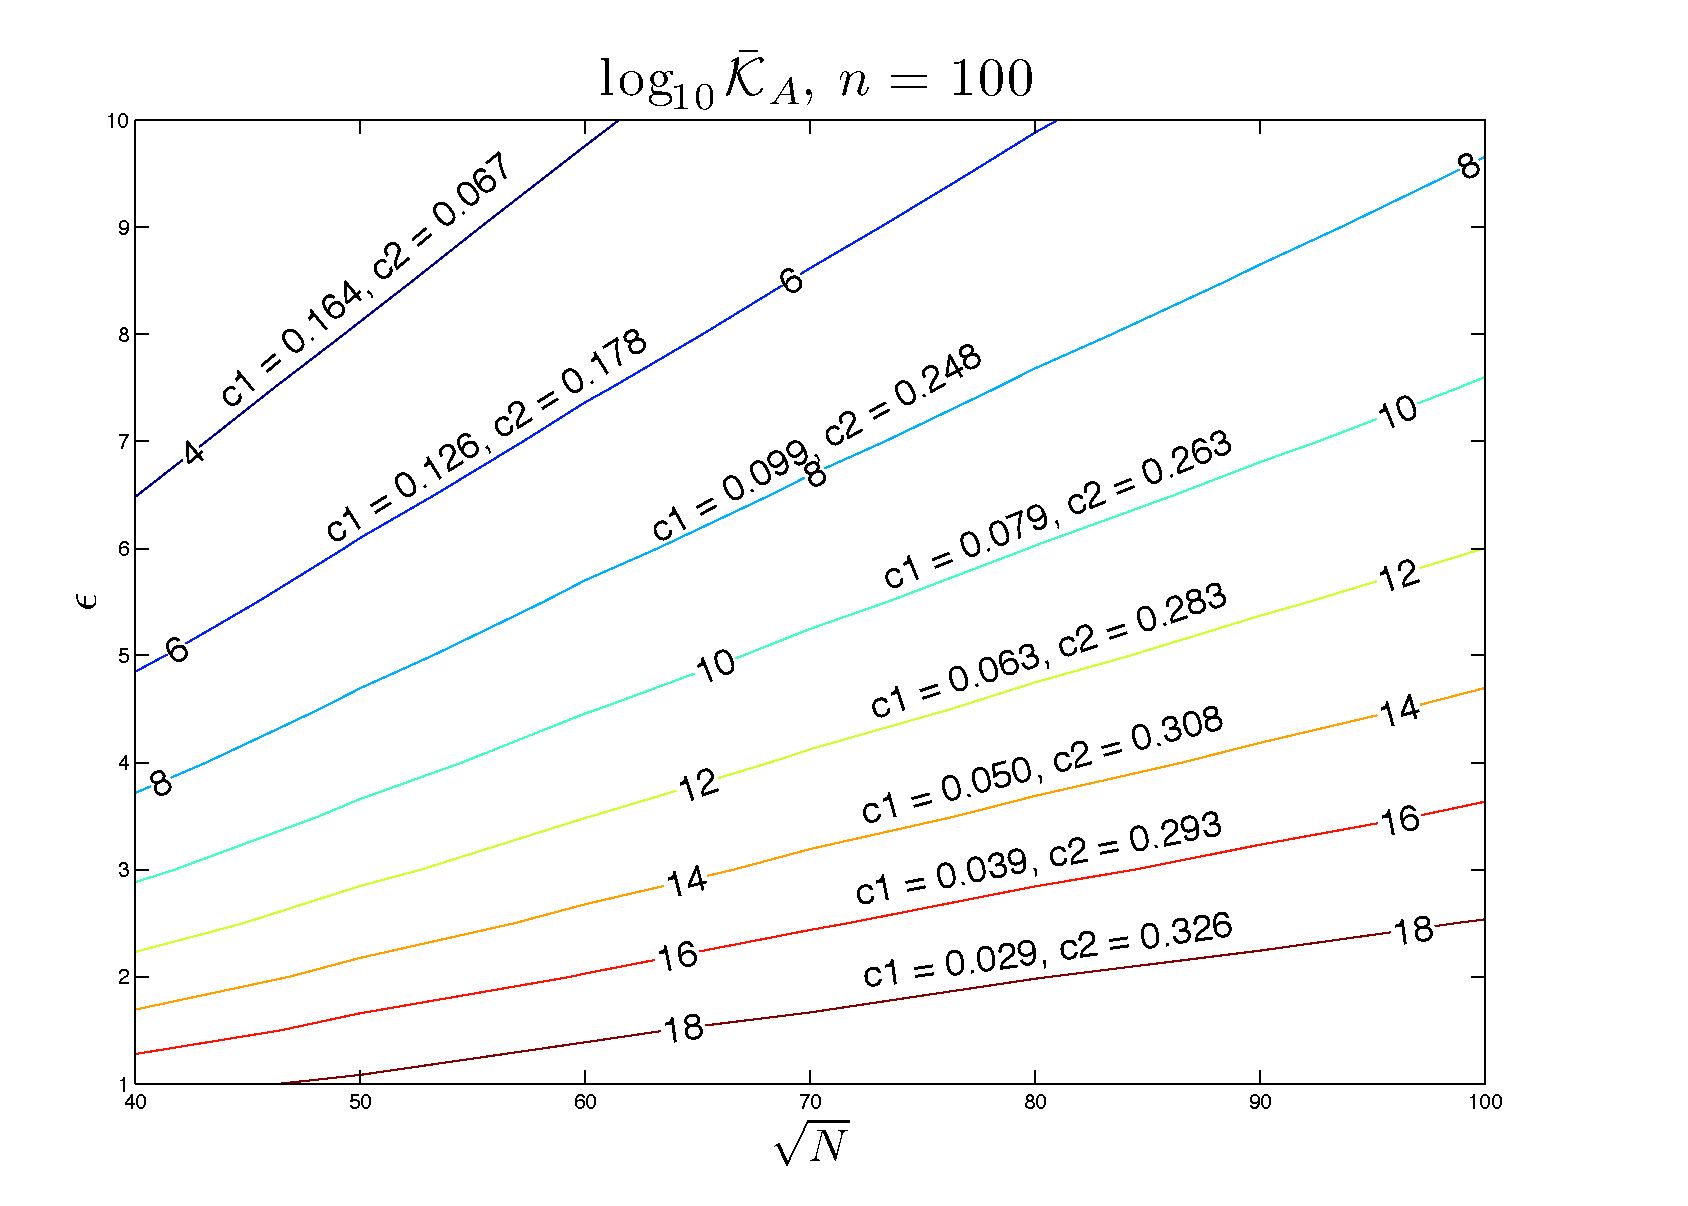
\includegraphics[width=0.45\textwidth]{../figures/chapter2/epsilon_contours/labeled_contour_n100.pdf}
\caption{Contours for choosing $\epsilon$ for $n=20$, 40, 60, 80 and 100 on the unit sphere as a function of $\sqrt{N}$. Contours assume near uniform distribution of nodes (e.g., maximum determinant nodes, icosahedral grids and spherical centroidal voronoi tessellations). Superimposed above each contour are parameters for the linear regression of the line, $c_{1} \sqrt{N} - c_{2}$. }
\label{fig:epsilon_contours}
\end{figure}



}

%\part{Appendices}
%\appendix
%The following appendices are included to illuminate subtleties of the RBF-FD method. The first discusses the method's ability to avoid pole singularities when applied to solid body transport on the sphere. The second considers the difference between directly computing weights for differentiation operators versus leveraging linear combinations of weights to indirectly construct the same operators. 
%%\makeatletter
%\@ifundefined{standalonetrue}{\newif\ifstandalone}{}
%\@ifundefined{section}{\standalonetrue}{\standalonefalse}
%\makeatother
%\ifstandalone
%\documentclass{report}
%
%\usepackage{textcase}
%\usepackage{hyperref}
%\hypersetup{breaklinks=true}


% Added packages
\usepackage[usenames]{color}
\usepackage{amsfonts, amsmath, amssymb, graphics}

% NOTE: bibentry MUST appear before the hyperref or build will fail
\usepackage{bibentry}
\nobibliography*
\usepackage[square,sort,comma,numbers]{natbib}
  
\usepackage{float}
\usepackage[
	hidelinks,%
    %hyperindex=true,		% Make numbers of index links as well
   	backref=page, 		% Provide page listing where refs occur in the bibliography
	%breaklinks=true,
    %colorlinks,%
    %citecolor=green,%
    %filecolor=blue,%
    %linkcolor=red,%
    %urlcolor=red, 
]{hyperref}

\usepackage{dsfont}
%%%% USEPACKAGES for MACROS %%%%%
\usepackage{algpseudocode}
\usepackage[chapter]{algorithm}
%\usepackage{caption}
\usepackage{subcaption}
\usepackage{url}

\usepackage{array}
\usepackage{arydshln}
\usepackage{multirow}
\usepackage{multicol}
%\usepackage[section]{placeins}

\usepackage[usenames,dvipsnames]{color}
%\usepackage[english]{babel}
\usepackage{tabularx}
\usepackage{soul}
\usepackage{xparse}
\usepackage{listings}
%\usepackage[normalem]{ulem}



%%%%%%%%%%%%%%%
% Show a list of items "todo" or "done" 
% USAGE: 
% \begin{todolist} 
% 	\todo Something not finished
% 	\done Something finished
% \end{todolist} 
\newenvironment{todolist}{%
  \begin{list}{}{}% whatever you want the list to be
  \let\olditem\item
  \renewcommand\item{\olditem \textcolor{red}{(TODO)}: }
  \newcommand\todo{\olditem \textcolor{red}{(TODO)}: }
   \newcommand\done{\olditem \textcolor{ForestGreen}{(DONE)}: }
}{%
  \end{list}
} 
%%%%%%%%%%%%%%%

%%%%%%%%%%%%%%%
% Show a Author's Note
% USAGE: 
% \incomplete[Optional footnote message to further clarify note]{The text which is currently not finished}
\DeclareDocumentCommand \incomplete{ o m }
{%
\IfNoValueTF {#1}
{\textcolor{red}{Incomplete: \ul{#2}}} 
{\textcolor{red}{Incomplete: \ul{#2}}\footnote{Comment: #1}}%
}
%%%%%%%%%%%%%%%



%%%%%%%%%%%%%%%
% Show a Author's Note
% USAGE: 
% \authnote[Optional footnote message to further clarify note]{The note to your readers}
\DeclareDocumentCommand \authnote { o m }
{%
\IfNoValueTF {#1}
{\textcolor{blue}{Author's Note: \ul{#2}}} 
{\textcolor{blue}{Author's Note: \ul{#2}}\footnote{Comment: #1}}%
}
%%%%%%%%%%%%%%%



%%%%%%%%%%%%%%%
% Strike out text that doesn't belong in the paper
% USAGE: 
% \strike[Optional footnote to state why it doesn't belong]{Text to strike out}
\DeclareDocumentCommand \strike { o m }
{%
\setstcolor{Red}
\IfNoValueTF {#1}
{\textcolor{Gray}{\st{#2}}} 
{\textcolor{Gray}{\st{#2}}\footnote{Comment: #1}}%
}
%%%%%%%%%%%%%%%

\definecolor{light-gray}{gray}{0.95}

\newcommand{\cbox}[3]{
\ \\
\fcolorbox{#1}{#2}{
\parbox{\textwidth}{
#3
}
}
}

% Setup an environment similar to verbatim but which will highlight any bash commands we have
\lstnewenvironment{unixcmds}[0]
{
%\lstset{language=bash,frame=shadowbox,rulesepcolor=\color{blue}}
\lstset{ %
language=sh,		% Language
basicstyle=\ttfamily,
backgroundcolor=\color{light-gray}, 
rulecolor=\color{blue},
%frame=tb, 
columns=fullflexible,
%framexrightmargin=-.2\textwidth,
linewidth=0.8\textwidth,
breaklines=true,
%prebreak=/, 
  prebreak = \raisebox{0ex}[0ex][0ex]{\ensuremath{\hookleftarrow}},
%basicstyle=\footnotesize,       % the size of the fonts that are used for the code
%numbers=left,                   % where to put the line-numbers
%numberstyle=\footnotesize,      % the size of the fonts that are used for the line-numbers
%stepnumber=2,                   % the step between two line-numbers. If it's 1 each line 
                                % will be numbered
%numbersep=5pt,                  % how far the line-numbers are from the code
showspaces=false,               % show spaces adding particular underscores
showstringspaces=false,         % underline spaces within strings
showtabs=false,                 % show tabs within strings adding particular underscores
frame=single,	                % adds a frame around the code
tabsize=2,	                % sets default tabsize to 2 spaces
captionpos=b,                   % sets the caption-position to bottom
breakatwhitespace=false,        % sets if automatic breaks should only happen at whitespace
}
} { }

% Setup an environment similar to verbatim but which will highlight any bash commands we have
\lstnewenvironment{cppcode}[1]
{
%\lstset{language=bash,frame=shadowbox,rulesepcolor=\color{blue}}
\lstset{ %
	backgroundcolor=\color{light-gray}, 
	rulecolor=\color[rgb]{0.133,0.545,0.133},
	tabsize=4,
	language=[GNU]C++,
%	basicstyle=\ttfamily,
        basicstyle=\scriptsize,
        upquote=true,
        aboveskip={1.5\baselineskip},
        columns=fullflexible,
        %framexrightmargin=-.1\textwidth,
       %framexleftmargin=6mm,
        showstringspaces=false,
        extendedchars=true,
        breaklines=true,
        prebreak = \raisebox{0ex}[0ex][0ex]{\ensuremath{\hookleftarrow}},
        frame=single,
        showtabs=false,
        showspaces=false,
        showstringspaces=false,
        numbers=left,                   % where to put the line-numbers
	numberstyle=\footnotesize,      % the size of the fonts that are used for the line-numbers
	stepnumber=4,                   % the step between two line-numbers. If it's 1 each line 
                                % will be numbered
	firstnumber=#1,
         numbersep=5pt,                  % how far the line-numbers are from the code
        identifierstyle=\ttfamily,
        keywordstyle=\color[rgb]{0,0,1},
        commentstyle=\color[rgb]{0.133,0.545,0.133},
        stringstyle=\color[rgb]{0.627,0.126,0.941},
}
} { }

% Setup an environment similar to verbatim but which will highlight any bash commands we have
\lstnewenvironment{mcode}[1]
{
\lstset{ %
	backgroundcolor=\color{light-gray}, 
	rulecolor=\color[rgb]{0.133,0.545,0.133},
	tabsize=4,
	language=Matlab,
%	basicstyle=\ttfamily,
        basicstyle=\scriptsize,
        upquote=true,
        aboveskip={1.5\baselineskip},
        columns=fullflexible,
        %framexrightmargin=-.1\textwidth,
       %framexleftmargin=6mm,
        showstringspaces=false,
        extendedchars=true,
        breaklines=true,
        prebreak = \raisebox{0ex}[0ex][0ex]{\ensuremath{\hookleftarrow}},
        frame=single,
        showtabs=false,
        showspaces=false,
        showstringspaces=false,
        numbers=left,                   % where to put the line-numbers
	numberstyle=\footnotesize,      % the size of the fonts that are used for the line-numbers
	stepnumber=4,                   % the step between two line-numbers. If it's 1 each line 
                                % will be numbered
	firstnumber=#1,
         numbersep=5pt,                  % how far the line-numbers are from the code
        identifierstyle=\ttfamily,
        keywordstyle=\color[rgb]{0,0,1},
        commentstyle=\color[rgb]{0.133,0.545,0.133},
        stringstyle=\color[rgb]{0.627,0.126,0.941},
}
} { }

\newcommand{\inputmcode}[1]{%
\lstset{ %
	backgroundcolor=\color{light-gray},  %
	rulecolor=\color[rgb]{0.133,0.545,0.133}, %
	tabsize=4, %
	language=Matlab, %
%	basicstyle=\ttfamily,
        basicstyle=\scriptsize, %
        %        upquote=true,
        aboveskip={1.5\baselineskip}, %
        columns=fullflexible, %
        %framexrightmargin=-.1\textwidth,
       %framexleftmargin=6mm,
        showstringspaces=false, %
        extendedchars=true, %
        breaklines=true, %
        prebreak = \raisebox{0ex}[0ex][0ex]{\ensuremath{\hookleftarrow}}, %
        frame=single, %
        showtabs=false, %
        showspaces=false, %
        showstringspaces=false,%
        numbers=left,                   % where to put the line-numbers
	numberstyle=\footnotesize,      % the size of the fonts that are used for the line-numbers
	stepnumber=4,                   % the step between two line-numbers. If it's 1 each line 
                                % will be numbered
         numbersep=5pt,                  % how far the line-numbers are from the code
        identifierstyle=\ttfamily, %
        keywordstyle=\color[rgb]{0,0,1}, %
        commentstyle=\color[rgb]{0.133,0.545,0.133}, %
        stringstyle=\color[rgb]{0.627,0.126,0.941} %
}
\lstinputlisting{#1}%
}

%\lstset{ %
%	backgroundcolor=\color{light-gray}, 
%	rulecolor=\color[rgb]{0.133,0.545,0.133},
%	tabsize=4,
%	language=Matlab,
%%	basicstyle=\ttfamily,
%        basicstyle=\scriptsize,
%        upquote=true,
%        aboveskip={1.5\baselineskip},
%        columns=fullflexible,
%        %framexrightmargin=-.1\textwidth,
%       %framexleftmargin=6mm,
%        showstringspaces=false,
%        extendedchars=true,
%        breaklines=true,
%        prebreak = \raisebox{0ex}[0ex][0ex]{\ensuremath{\hookleftarrow}},
%        frame=single,
%        showtabs=false,
%        showspaces=false,
%        showstringspaces=false,
%        numbers=left,                   % where to put the line-numbers
%	numberstyle=\footnotesize,      % the size of the fonts that are used for the line-numbers
%	stepnumber=4,                   % the step between two line-numbers. If it's 1 each line 
%                                % will be numbered
%	firstnumber=#1,
%         numbersep=5pt,                  % how far the line-numbers are from the code
%        identifierstyle=\ttfamily,
%        keywordstyle=\color[rgb]{0,0,1},
%        commentstyle=\color[rgb]{0.133,0.545,0.133},
%        stringstyle=\color[rgb]{0.627,0.126,0.941},
%}


\newcommand{\Laplacian}[1]{\nabla^2 #1}

% set of all nodes received and contained on GPU
\newcommand{\setAllNodes}[0]{\mathcal{G}}
% set of stencil centers on GPU
\newcommand{\setCenters}[0]{\mathcal{Q}}
% set of stencil centers with nodes in \setDepend
\newcommand{\setBoundary}[0]{\mathcal{B}}
% set of nodes received by other GPUs
\newcommand{\setDepend}[0]{\mathcal{R}}
% set of nodes sent to other GPUs
\newcommand{\setProvide}[0]{\mathcal{O}}


\newcommand{\toprule}[0]{\hline}
\newcommand{\midrule}[0]{\hline\hline}
\newcommand{\bottomrule}[0]{\hline}

\newcolumntype{C}{>{\centering\arraybackslash}b{1in}}
\newcolumntype{L}{>{\flushleft\arraybackslash}b{1.5in}}
\newcolumntype{R}{>{\flushright\arraybackslash}b{1.5in}}
\newcolumntype{D}{>{\flushright\arraybackslash}b{2.0in}}
\newcolumntype{E}{>{\flushright\arraybackslash}b{1.0in}}

\DeclareSymbolFont{AMSb}{U}{msb}{m}{n}
\DeclareMathSymbol{\N}{\mathbin}{AMSb}{"4E}
\DeclareMathSymbol{\Z}{\mathbin}{AMSb}{"5A}
\DeclareMathSymbol{\R}{\mathbin}{AMSb}{"52}
\DeclareMathSymbol{\Q}{\mathbin}{AMSb}{"51}
\DeclareMathSymbol{\PP}{\mathbin}{AMSb}{"50}
\DeclareMathSymbol{\I}{\mathbin}{AMSb}{"49}
%\DeclareMathSymbol{\C}{\mathbin}{AMSb}{"43}

%%%%%% VECTOR NORM: %%%%%%%
\newcommand{\vectornorm}[1]{\left|\left|#1\right|\right|}
\newcommand{\vnorm}[1]{\left|\left|#1\right|\right|}
\newcommand{\by}[0]{\times}
\newcommand{\vect}[1]{\mathbf{#1}}
%\newcommand{\mat}[1]{\mathbf{#1}} 

%\renewcommand{\vec}[1]{ \textbf{#1} }
%%%%%%%%%%%%%%%%%%%%%%

%%%%%%% THM, COR, DEF %%%%%%%
%\newtheorem{theorem}{Theorem}[section]
%\newtheorem{lemma}[theorem]{Lemma}
%\newtheorem{proposition}[theorem]{Proposition}
%\newtheorem{corollary}[theorem]{Corollary}
%\newenvironment{proof}[1][Proof]{\begin{trivlist}
%\item[\hskip \labelsep {\bfseries #1}]}{\end{trivlist}}
%\newenvironment{definition}[1][Definition]{\begin{trivlist}
%\item[\hskip \labelsep {\bfseries #1}]}{\end{trivlist}}
%\newenvironment{example}[1][Example]{\begin{trivlist}
%\item[\hskip \labelsep {\bfseries #1}]}{\end{trivlist}}
%\newenvironment{remark}[1][Remark]{\begin{trivlist}
%\item[\hskip \labelsep {\bfseries #1}]}{\end{trivlist}}
%\newcommand{\qed}{\nobreak \ifvmode \relax \else
%      \ifdim\lastskip<1.5em \hskip-\lastskip
%      \hskip1.5em plus0em minus0.5em \fi \nobreak
%      \vrule height0.75em width0.5em depth0.25em\fi}
%%%%%%%%%%%%%%%%%%%%%%

%
%\usepackage[algochapter]{algorithm2e}
%\usepackage[usenames]{color}
% colors to show the corrections
\newcommand{\red}[1]{\textbf{\textcolor{red}{#1}}}
\newcommand{\blue}[1]{\textbf{\textcolor{blue}{#1}}}
\newcommand{\cyan}[1]{\textbf{\textcolor{cyan}{#1}}}
\newcommand{\green}[1]{\textbf{\textcolor{green}{#1}}}
\newcommand{\magenta}[1]{\textbf{\textcolor{magenta}{#1}}}
\newcommand{\orange}[1]{\textbf{\textcolor{orange}{#1}}}
%%%%%%%%%% DK DK
% comments between authors
\newcommand{\toall}[1]{\textbf{\green{@@@ All: #1 @@@}}}
\newcommand{\toevan}[1]{\textbf{\red{*** Evan: #1 ***}}}
%\newcommand{\toevan}[1]{}  % USE FOR FINAL VERSION
\newcommand{\toe}[1]{\textbf{\red{*** Evan: #1 ***}}}
\newcommand{\tog}[1]{\textbf{\blue{*** Gordon: #1 ***}}}
%\newcommand{\togordon}[1]{\textbf{\blue{*** Gordon: #1 ***}}}
\renewcommand{\ge}[3]{{\textcolor{blue}{*** \textbf{Gordon:}\strike{#1} #2 ***}}\red{(#3)}}
\renewcommand{\ge}[3]{{\textcolor{blue}{#2}}}
\renewcommand{\ge}[3]{{\textcolor{Red}{#2}}}
\newcommand{\eb}[3]{{\textcolor{Red}{*** \textbf{Evan:}\strike{#1} #2 ***}}\red{(#3)}}
\renewcommand{\eb}[3]{{{\textcolor{Red}{#2}}}}
%\def\ge#1#2#3{}{\textbf{\blue{*** Gordon: #2 ***}}}{(#3)}
\newcommand{\gee}[1]{{\bf{\blue{{\em #1}}}}}
\newcommand{\old}[1]{}
\newcommand{\del}[1]{***#1*** }



% \DeclareMathOperator{\Sample}{Sample}
%\let\vaccent=\v % rename builtin command \v{} to \vaccent{}
%\renewcommand{\vec}[1]{\ensuremath{\mathbf{#1}}} % for vectors
\newcommand{\gv}[1]{\ensuremath{\mbox{\boldmath$ #1 $}}} 
% for vectors of Greek letters
\newcommand{\uv}[1]{\ensuremath{\mathbf{\hat{#1}}}} % for unit vector
\newcommand{\abs}[1]{\left| #1 \right|} % for absolute value
\newcommand{\avg}[1]{\left< #1 \right>} % for average
\let\underdot=\d % rename builtin command \d{} to \underdot{}
\renewcommand{\d}[2]{\frac{d #1}{d #2}} % for derivatives
\newcommand{\dd}[2]{\frac{d^2 #1}{d #2^2}} % for double derivatives
\newcommand{\pd}[2]{\frac{\partial #1}{\partial #2}} 
% for partial derivatives
\newcommand{\pdd}[2]{\frac{\partial^2 #1}{\partial #2^2}} 
\newcommand{\pdda}[3]{\frac{\partial^2 #1}{\partial #2 \partial #3}} 
% for double partial derivatives
\newcommand{\pdc}[3]{\left( \frac{\partial #1}{\partial #2}
 \right)_{#3}} % for thermodynamic partial derivatives
\newcommand{\ket}[1]{\left| #1 \right>} % for Dirac bras
\newcommand{\bra}[1]{\left< #1 \right|} % for Dirac kets
\newcommand{\braket}[2]{\left< #1 \vphantom{#2} \right|
 \left. #2 \vphantom{#1} \right>} % for Dirac brackets
\newcommand{\matrixel}[3]{\left< #1 \vphantom{#2#3} \right|
 #2 \left| #3 \vphantom{#1#2} \right>} % for Dirac matrix elements
\newcommand{\grad}[1]{\gv{\nabla} #1} % for gradient
\let\divsymb=\div % rename builtin command \div to \divsymb
\renewcommand{\div}[1]{\gv{\nabla} \cdot #1} % for divergence
\newcommand{\curl}[1]{\gv{\nabla} \times #1} % for curl
\let\baraccent=\= % rename builtin command \= to \baraccent
\renewcommand{\=}[1]{\stackrel{#1}{=}} % for putting numbers above =
\newcommand{\diffop}[1]{\mathcal{L}#1}
\newcommand{\boundop}[1]{\mathcal{B}#1}
\newcommand{\rvec}[0]{{\bf r}}

\newcommand{\Interior}[0]{\Omega}
\newcommand{\domain}[0]{\Omega}
%\newcommand{\Boundary}[0]{\partial \Omega}
\newcommand{\Boundary}[0]{\Gamma}

\newcommand{\on}[1]{\hskip1.5em \textrm{ on } #1}

\newcommand{\gemm}{\texttt{GEMM}}
\newcommand{\trmm}{\texttt{TRMM}}
\newcommand{\gesvd}{\texttt{GESVD}}
\newcommand{\geqrf}{\texttt{GEQRF}}


\newcommand{\minitab}[2][l]{\begin{tabular}{#1}#2\end{tabular}}
\newcommand{\comm}[1]{\textcolor{red}{\textit{#1}}}

\newcommand{\nfrac}[2]{
\nicefrac{#1}{#2}
%\frac{#1}{#2}
}

\usepackage{xparse}
\usepackage{soul}


%%%%%%%%%%%%%%%
% Show a Author's Note
% USAGE: 
% \incomplete[Optional footnote message to further clarify note]{The text which is currently not finished}
\DeclareDocumentCommand \incomplete{ o m }
{%
\IfNoValueTF {#1}
{\textcolor{red}{Incomplete: \ul{#2}}} 
{\textcolor{red}{Incomplete: \ul{#2}}\footnote{Comment: #1}}%
}
%%%%%%%%%%%%%%%



%%%%%%%%%%%%%%%
% Show a Author's Note
% USAGE: 
% \authnote[Optional footnote message to further clarify note]{The note to your readers}
\DeclareDocumentCommand \authnote { o m }
{%
\IfNoValueTF {#1}
{\textcolor{blue}{Author's Note: \ul{#2}}} 
{\textcolor{blue}{Author's Note: \ul{#2}}\footnote{Comment: #1}}%
}
%%%%%%%%%%%%%%%



%%%%%%%%%%%%%%%
% Strike out text that doesn't belong in the paper
% USAGE: 
% \strike[Optional footnote to state why it doesn't belong]{Text to strike out}
\DeclareDocumentCommand \strike { o m }
{%
\setstcolor{red}
\IfNoValueTF {#1}
{\textcolor{Gray}{\st{#2}}} 
{\textcolor{Gray}{\st{#2}}\footnote{Comment: #1}}%
}
%%%%%%%%%%%%%%%



%
% colors to show the corrections
\newcommand{\red}[1]{\textbf{\textcolor{red}{#1}}}
\newcommand{\blue}[1]{\textbf{\textcolor{blue}{#1}}}
\newcommand{\cyan}[1]{\textbf{\textcolor{cyan}{#1}}}
\newcommand{\green}[1]{\textbf{\textcolor{green}{#1}}}
\newcommand{\magenta}[1]{\textbf{\textcolor{magenta}{#1}}}
\newcommand{\orange}[1]{\textbf{\textcolor{orange}{#1}}}
%%%%%%%%%% DK DK
% comments between authors
\newcommand{\toall}[1]{\textbf{\green{@@@ All: #1 @@@}}}
\newcommand{\toevan}[1]{\textbf{\red{*** Evan: #1 ***}}}
%\newcommand{\toevan}[1]{}  % USE FOR FINAL VERSION
\newcommand{\toe}[1]{\textbf{\red{*** Evan: #1 ***}}}
\newcommand{\tog}[1]{\textbf{\blue{*** Gordon: #1 ***}}}
%\newcommand{\togordon}[1]{\textbf{\blue{*** Gordon: #1 ***}}}
\renewcommand{\ge}[3]{{\textcolor{blue}{*** \textbf{Gordon:}\strike{#1} #2 ***}}\red{(#3)}}
\renewcommand{\ge}[3]{{\textcolor{blue}{#2}}}
\renewcommand{\ge}[3]{{\textcolor{red}{#2}}}
\newcommand{\eb}[3]{{\textcolor{red}{*** \textbf{Evan:}\strike{#1} #2 ***}}\red{(#3)}}
\renewcommand{\eb}[3]{{{\textcolor{red}{#2}}}}
%\def\ge#1#2#3{}{\textbf{\blue{*** Gordon: #2 ***}}}{(#3)}
\newcommand{\gee}[1]{{\bf{\blue{{\em #1}}}}}
\newcommand{\old}[1]{}
\newcommand{\del}[1]{***#1*** }



% Rename  this file          misc_mac.tex
%----------------------------------------------------------------------
%%%%%%%%%%%%%%%%%%%%%%%%%%%%%%%%%%%%%%%%%%%%%%%%%%%%%%%%%%%%%%%%%%%%%%%%%%%%%%%
%
%	Math Symbols   Math Symbols   Math Symbols   Math Symbols   
%
%%%%%%%%%%%%%%%%%%%%%%%%%%%%%%%%%%%%%%%%%%%%%%%%%%%%%%%%%%%%%%%%%%%%%%%%%%%%%%%
\def\pmb#1{\setbox0=\hbox{$#1$}%
	\kern-.025em\copy0\kern-\wd0
	\kern.05em\copy0\kern-\wd0
	\kern-.025em\raise.0433em\box0}
\def\pmbf#1{\pmb#1}
\def\bfg#1{\pmb#1}

% BETTER VALUES FOR AUTOMATIC FIGURE PLACEMENT THAN THOSE PROVIDED BY 
% LATEX DEFAULTS.

\renewcommand{\textfloatsep}{1ex}
\renewcommand{\floatpagefraction}{0.9}
\renewcommand{\intextsep}{1ex}
\renewcommand{\topfraction}{.9}
\renewcommand{\bottomfraction}{.9}
\renewcommand{\textfraction}{.1}

% #1  position of floating figure (h|t|b|p)
% #1  EPS postscript file
% #2  size
% #3  caption

%usage of newfig:
%  \newfig{file.ps}{3in}{Fig1: this is a figure}

\input{epsf}
\def\newfig#1#2#3{
  \begin{figure}[htbp]
  \vspace{1ex}
  \setlength{\epsfxsize}{#2}
  \centerline{\epsfbox{#1}}
  \vspace{-.1in}\caption{\small #3}\break\vspace{.2in}
  \label{#1}
  \end{figure}
}

%usage of newfigtwo: 2 figures, vertically stacked
% \newfig
%	{file1.ps}
%	{file2.ps}
%	{width}
%	{vertical space}
%	{Caption}

\def\newfigtwo#1#2#3#4#5{
  \begin{figure}[htbp]
  \vspace{1ex}
  \setlength{\epsfxsize}{#3}
  \centerline{\epsfbox{#1}}
  \vspace{#4}
  \setlength{\epsfxsize}{#3}
  \centerline{\epsfbox{#2}}
  \vspace{-.1in}\caption{\small #5}\break\vspace{.2in}
  \label{#1}
  \end{figure}
}

\def\newfigh#1#2#3#4{  % add height specification
  \begin{figure}[htbp]
  \vspace{1ex}
  \setlength{\epsfxsize}{#2}
  \setlength{\epsfysize}{#4}
  \centerline{\epsfbox{#1}}
  \vspace{-.1in}\caption{\small #3}\break\vspace{.2in}
  \label{#1}
  \end{figure}
}

\def\herefig#1#2#3{
  \begin{figure}[h]
  \setlength{\epsfxsize}{#2}
  \centerline{\epsfbox{#1}}
  \caption{\small #3}
  \label{#1}
  \end{figure}
}

\def\etal{{{\em et~al.\,\,}}}
\def\note#1{\\ =====#1===== \\}
\def\FBOX#1{\ \\ \fbox{\begin{minipage}{5in}#1\end{minipage}}\\ }
\newcount\sectionno     \sectionno=0
\newcount\eqnum         \eqnum=0
\def\addeqno{\global\advance \eqnum by  1 }
\def\subeqno{\global\advance \eqnum by -1 }
%\def\eqn{\addeqno \eqno \hbox{(\number\sectionno.\number\eqnum)} }

\def\tildetilde#1{\tilde{\tilde{#1}}}
\def\barbar#1{\overbar{\overbar{#1}}}

\def\vsp#1{\vspace{#1 ex}}
\def\fpar{\hspace{\parindent}}
%
%  \pf : 2 arguments: numerator and denominator of partial derivative
%
\def\pf#1#2{{\frac{\partial{#1}}{\partial{#2}}}}
\def\pfs#1#2{{\partial_{#2}{#1}}}
\def\pftwo#1#2{{\frac{\partial^2{#1}}{\partial{#2}^2}}}
\def\pfxx#1#2{{\frac{\partial^2{#1}}{\partial{#2}^2}}}
%\def\pfxy#1#2{{\frac{\partial^2{#1}}{\partial{#2}\partial{#3}}}}
\def\pfn#1#2#3{{\frac{\partial^{#1}{#2}}{\partial{#3}^{#1}}}}
\def\df#1#2{{\frac{d{#1}}{d{#2}}}}
\def\dfn#1#2#3{{\frac{d^{#1}{#2}}{d{#3}^{#1}}}}
\def\Dt#1#2{\frac{D#1}{D#2}}
\def\dt#1#2{\frac{d#1}{d#2}}
\def\bld#1{{\bf #1}}
\def\pfp#1#2#3{\pf{}{#3}{\left(\frac{#1}{#2}\right)}}

\def\norm#1{\|#1\|}

%
% Graphic characters  (\dot already defined by TeX/LateX)
%
\def\dash{\rule[1.5pt]{2mm}{.3mm}\HS{.9mm}}
\def\dott{\rule[1.5pt]{.7mm}{.3mm}\HS{.7mm}}
\def\dashline{\dash\dash\dash}
\def\dotline{\dott\dott\dott\dott\dott\dott}
\def\dashdotline{\dash$\cdot$\HS{.9mm}\dash}
\def\solidline{\rule[2pt]{7mm}{.3mm}}
% 
% overcircle
%
\def\ovcircle#1{\buildrel{\circ}\over{#1}}
%\def\below#1#2{\buildrel{#2}\under{#1}}
%\def\above#1#2{\buildrel{#2}\over{#1}}
%
%  big parenthesis and brackets
%
\def\bigpar#1#2{{\left(\frac{#1}{#2}\right)}}
\def\bigbra#1#2{{\left\[\frac{#1}{#2}\right\]}}

\def\Lp{\left(}
\def\Rp{\right)}
\def\Lb{\left[}
\def\Rb{\right]}
\def\Ln{\left\langle}
\def\Rn{\right\rangle}
\def\Ld{\left.}
\def\Rd{\right.}
\def\Lv{\left|}
\def\Rv{\right|}
\def\Lbr{\left|}
\def\Rbr{\right|}
\def\lng{\langle}
\def\rng{\rangle}
\def\Lc{\left\{}
\def\Rc{\right\}}
%%% %

% Cannot be handled by Lyx
%\def\[{{[}}
%\def\]{{]}}

%
\def\eol{\nonumber \\}
\def\eolnonb{\nonumber\\}
\def\eolnb{\\}
\def\nonb{\nonumber}
\def\be{\begin{equation}}
\def\ee{\end{equation}}
\def\BEQNA{\begin{eqnarray}}
\def\EEQNA{\end{eqnarray}}
\def\eqa{&=&}
\def\beqna{\begin{eqnarray}}
\def\eeqna{\end{eqnarray}}
\def\bverb{\begin{verbatim}}
\def\everb{\end{verbatim}}
\def\VERB#1{\bverb #1 \everb}
\def\btbl{\begin{tabular}}
\def\etbl{\end{tabular}}
\def\bmini{\begin{minipage}[t]{5.5in}}
\def\emini{\end{minipage}}
\def\parray#1#2{\left(\begin{array}{#1}#2\end{array}\right)}
\def\barray#1#2{\left[\begin{array}{#1}#2\end{array}\right]}
\def\carray#1#2{\left\{\begin{array}{#1}#2\end{array}\right.}
\def\darray#1#2{\left|\begin{array}{#1}#2\end{array}\right|}

\def\BEGTABLE#1{\begin{table}[hbt]\vspace{2ex}\begin{center}\bmini\centering\btbl{#1}}
\def\ENDTABLE#1#2{\etbl\caption[#1]{#2}\EMINI\end{center}\vspace{2ex}\end{table}}

\def\bfltbl#1{\begin{table}[hbt]\vspace{2ex}\begin{center}\bmini\centering\btbl{#1}}
\def\efltbl#1#2{\etbl\caption[#1]{#2}\emini\end{center}\vspace{2ex}\end{table}}
\def\mcol{\multicolumn}
%
%  label equations with (#)
%
\def\reff#1{(\ref{#1})}
%
%  macros borrowed from viewgraph package
%

\newenvironment{LETTRS}[3]{\begin{letter}{#1}
\input{origin}\opening{Dear #2:}\input{#3}\closing{Sincerely yours,}\end{letter}}{\clearpage}

\newenvironment{VIEW}[1]{{\BC\Huge\bf #1 \EC}\LARGE\VS{.05in}}{\clearpage}

\def\RM#1{\rm{#1\ }}
\def\BV{\begin{VIEW}}
\def\EV{\end{VIEW}}

\def\NI{\noindent}

\def\VS{\vspace*}
\def\HS{\hspace*}
\def\IT{\item}

\def\BARR{\begin{array}}
\def\EARR{\end{array}}

\def\BPARR{\left(\begin{array}}
\def\EPARR{\end{array}\right)}

\def\BDET{\left|\begin{array}}
\def\EDET{\end{array}\right|}

\def\BDF{\begin{definition}}
\def\EDF{\end{definition}}

\def\BSU{\begin{block}{Summary}}
\def\ESU{\end{block}}

\def\BEX{\begin{example}}
\def\EEX{\end{example}}

\def\BTH{\begin{theorem}}
\def\ETH{\end{theorem}}

\def\BCO{\begin{corollary}}
\def\ECO{\end{corollary}}

\def\BPROOF{\begin{proof}}
\def\EPROOF{\end{proof}}

\def\BLM{\begin{lemma}}
\def\ELM{\end{lemma}}

\def\BEQ{\begin{equation}}
\def\EEQ{\end{equation}}

\def\BEQNNB{$$}
\def\EEQNNB{$$}

\def\BE{\begin{enumerate}}
\def\EE{\end{enumerate}}

\def\BD{\begin{description}}
\def\ED{\end{description}}

\def\BI{\begin{itemize}}
\def\EI{\end{itemize}}

\def\BC{\begin{center}}
\def\EC{\end{center}}

\def\BFIG{\begin{figure}}
\def\EFIG{\end{figure}}

\def\BTABB{\begin{tabbing}}
\def\ETABB{\end{tabbing}}

\def\BMINI{\begin{minipage}}
\def\EMINI{\end{minipage}}

\def\BTABLE{\begin{table}}
\def\ETABLE{\end{table}}

\def\BTABUL{\begin{tabular}}
\def\ETABUL{\end{tabular}}

\def\MCOL{\multicolumn}
\def\UL{\underline}
\def\ULL#1{\UL{\UL{#1}}}

\def\BDOC{\begin{document}}
\def\EDOC{\end{document}}

\def\EM#1{{\em #1\/}}
\def\FN{\footnote}

% Courtesy of Ugo Piomelli

\def\latexfig #1 #2 #3 #4 #5 {\ \vfill
\hfill\hbox to 0.05in{\vbox to #3truein{
         \special{psfile="#1" angle=270 hscale=100 
                  hoffset=#4 voffset=#5 vscale=100} }\hfill}
\hfill\vspace{-0.1in}        }

% #1 is the .ps filename
% #2 is not used in the present version
% #3 is the size of the white space left above the caption (in inches)
% #4 is the horizontal offset from some unknown reference point.
%    It is in 1/72 of an inch and is positive to the right.
% #5 is the vertical offset from some unknown reference point.
%    It is in 1/72 of an inch and is positive upwards.


\newcommand{\mathsym}[1]{{}}
\newcommand{\unicode}[1]{{}}
\newcommand{\ep}{\epsilon}
\newcommand{\vv}{\mathbf{v}}
\newcommand{\vu}{\mathbf{u}}
\newcommand{\vx}{\mathbf{x}}

\newcommand{\Laplacian}[1]{\nabla^2 #1}
\newcommand{\LaplaceBeltrami}[1]{\Delta_S #1}

% set of all nodes received and contained on GPU
\newcommand{\setAllNodes}[0]{\mathcal{G}}
% set of stencil centers on GPU
\newcommand{\setCenters}[0]{\mathcal{Q}}
% set of stencil centers with nodes in \setDepend
\newcommand{\setBoundary}[0]{\mathcal{B}}
% set of nodes received by other GPUs
\newcommand{\setDepend}[0]{\mathcal{R}}
% set of nodes sent to other GPUs
\newcommand{\setProvide}[0]{\mathcal{O}}





\usepackage{tabularx} 
\newcolumntype{C}{>{\centering\arraybackslash}b{1in}}
\newcolumntype{L}{>{\flushleft\arraybackslash}b{1.5in}}
\newcolumntype{R}{>{\flushright\arraybackslash}b{1.5in}}
\newcolumntype{D}{>{\flushright\arraybackslash}b{2.0in}}
\newcolumntype{E}{>{\flushright\arraybackslash}b{1.0in}}


 


%\usepackage{xcolor}

%\usepackage{refcheck}
% Sepia
%\definecolor{myBGcolor}{HTML}{F6F0D6}
%\definecolor{myTextcolor}{HTML}{4F452C}
% Dark
%\definecolor{myBGcolor}{HTML}{3E3535}
%\definecolor{myTextcolor}{HTML}{CFECEC}
%\color{myTextcolor}
%\pagecolor{myBGcolor}
 
%
%\begin{document}
%\fi

\chapter{Avoiding Pole Singularities with RBF-FD}
This content follows \cite{FlyerWright07,FlyerWright09}. 

Within the test cases of this dissertation, we solve convective PDEs on the unit sphere with the form: 
$$
\pd{h}{t} = \vu \cdot \nabla h
$$
where $\vu$ is velocity. For example, the cosine bell advection has this particular form:
\begin{equation}
\pd{h}{t} = \frac{u}{\cos{\theta}} \pd{h}{\lambda} + v \pd{h}{\theta} \label{eq:cosine_bell_appendix}
\end{equation}
in the spherical coordinate system defined by
\begin{align*}
x & = \cos{\theta}\cos{\lambda} \\
y & = \cos{\theta}\sin{\lambda} \\
z & = \sin{\theta}
\end{align*}
where $\theta \in (-\frac{\pi}{2}, \frac{\pi}{2})$ is the elevation angle and $\lambda \in (-\pi,\pi)$ is the azimuthal angle.
Observe that as $\theta \rightarrow \pm \frac{\pi}{2}$, the $\frac{1}{\cos{\theta}}$ term goes to infinity as a discontinuity. 

One of the many selling points for RBF-FD and other RBF methods is their ability analytically avoid pole singularities, which arise from the choice of coordinate system and not from the methods themselves. Since RBFs are inherently based on Euclidean distance between nodes, and not geodesic distance, it is said that they do not ``feel'' the effects of the geometry or recognize singularities naturally inherent in the coordinate system \cite{FlyerWright07}. 
Here we demonstrate how pole singularities are analytically avoided with RBF-FD for cosine bell advection.  


Let $r = || \vx - \vx_j ||$ be the Euclidean distance which is invariant of the coordinate system. In Cartesian coordinates, we have
$$
r = \sqrt{(x-x_j)^2 + (y-y_j)^2 + (z-z_j)^2}.
$$
In spherical coordinates we have:
$$
r = \sqrt{2(1-\cos{\theta}\cos{\theta_j}\cos{(\lambda-\lambda_j)} - \sin{\theta}\sin{\theta_j})}.
$$

The RBF-FD operators for $\d{}{\lambda}, \d{}{\theta}$ are discretized with the chain rule: 

\begin{align}
\d{\phi_{j}(r)}{\lambda} = \d{r}{\lambda} \d{\phi_{j}(r)}{r} & = \frac{\cos{\theta}\cos{\theta_j}\sin{(\lambda - \lambda_j)}}{r} \d{\phi_j(r)}{r}, \label{eq:rbfffd_d_dlambda} \\
\d{\phi_{j}(r)}{\theta} = \d{r}{\theta} \d{\phi_{j}(r)}{r} & = \frac{\sin{\theta}\cos{\theta_j}\cos{(\lambda-\lambda_j)} - \cos{\theta}\sin{\theta_j}}{r} \d{\phi}{r}, \label{eq:rbfffd_d_dtheta}
\end{align}
where $\phi_{j}(r)$ is the RBF centered at $\vx_{j}$. 

Plugging \ref{eq:rbfffd_d_dlambda} and \ref{eq:rbfffd_d_dtheta} into \ref{eq:cosine_bell_appendix}, produces the following explicit form: 
\begin{align*}
\d{h}{t} = u(\cos{\theta_j}\sin{(\lambda - \lambda_j)} \frac{1}{r} \d{\phi_j}{r}) + v (\sin{\theta}\cos{\theta_j}\cos{(\lambda-\lambda_j)} - \cos{\theta}\sin{\theta_j} \frac{1}{r} \d{\phi}{r}) 
\end{align*}
where $\cos{\theta}$ from \ref{eq:rbfffd_d_dlambda} analytically cancels with the $\frac{1}{\cos{\theta}}$ in \ref{eq:cosine_bell_appendix}.


Then, formally, one would assemble differentiation matrices containing weights for the following operators: 
\begin{align}
\D_\lambda & = \cos{\theta_j}\sin{(\lambda - \lambda_j)} \frac{1}{r} \d{\phi_j}{r}, \label{eq:dm_lambda} \\
\D_\theta &=  \sin{\theta}\cos{\theta_j}\cos{(\lambda-\lambda_j)} - \cos{\theta}\sin{\theta_j} \frac{1}{r} \d{\phi}{r}, \label{eq:dm_theta}
\end{align} 
and solve the explicit method of lines problem:
$$
\d{h}{t} = u \D_\lambda h + v \D_\theta h
$$
where now the system is completely free of singularities at the poles \cite{FlyerWright09}. 

We note that the expression $\cos{(\frac{\pi}{2})}$ evaluates on some systems to a very small number rather than zero (e.g., $6.1(10^{-17}$) on the Keeneland system with the GNU gcc compiler). The small value in turn allows $\frac{1}{\cos{\theta}}$ to evaluate to a large value (e.g., $1.6(10^{16})$) rather than ``inf" or ``NaN". A large value allows the cosine terms to cancel in double precision, whereas an ``inf'' or ``NaN'' would corrupt the numerics. Rather than avoid placing nodes at the poles, or assuming the machine will numerically cancel the singularities, it is preferred to use operators \ref{eq:dm_lambda}, \ref{eq:dm_theta} on the RHS of Equation~\ref{eq:rbffd_weight_system} to compute RBF-FD weights. 

%
%\ifstandalone
%\bibliographystyle{plain}
%\bibliography{merged_references}
%\end{document}
%\else
%\expandafter\endinput
%\fi
%%\makeatletter
%\@ifundefined{standalonetrue}{\newif\ifstandalone}{}
%\@ifundefined{section}{\standalonetrue}{\standalonefalse}
%\makeatother
%\ifstandalone
%\documentclass{report}
%
%\usepackage{textcase}
%\usepackage{hyperref}
%\hypersetup{breaklinks=true}


% Added packages
\usepackage[usenames]{color}
\usepackage{amsfonts, amsmath, amssymb, graphics}

% NOTE: bibentry MUST appear before the hyperref or build will fail
\usepackage{bibentry}
\nobibliography*
\usepackage[square,sort,comma,numbers]{natbib}
  
\usepackage{float}
\usepackage[
	hidelinks,%
    %hyperindex=true,		% Make numbers of index links as well
   	backref=page, 		% Provide page listing where refs occur in the bibliography
	%breaklinks=true,
    %colorlinks,%
    %citecolor=green,%
    %filecolor=blue,%
    %linkcolor=red,%
    %urlcolor=red, 
]{hyperref}

\usepackage{dsfont}
%%%% USEPACKAGES for MACROS %%%%%
\usepackage{algpseudocode}
\usepackage[chapter]{algorithm}
%\usepackage{caption}
\usepackage{subcaption}
\usepackage{url}

\usepackage{array}
\usepackage{arydshln}
\usepackage{multirow}
\usepackage{multicol}
%\usepackage[section]{placeins}

\usepackage[usenames,dvipsnames]{color}
%\usepackage[english]{babel}
\usepackage{tabularx}
\usepackage{soul}
\usepackage{xparse}
\usepackage{listings}
%\usepackage[normalem]{ulem}



%%%%%%%%%%%%%%%
% Show a list of items "todo" or "done" 
% USAGE: 
% \begin{todolist} 
% 	\todo Something not finished
% 	\done Something finished
% \end{todolist} 
\newenvironment{todolist}{%
  \begin{list}{}{}% whatever you want the list to be
  \let\olditem\item
  \renewcommand\item{\olditem \textcolor{red}{(TODO)}: }
  \newcommand\todo{\olditem \textcolor{red}{(TODO)}: }
   \newcommand\done{\olditem \textcolor{ForestGreen}{(DONE)}: }
}{%
  \end{list}
} 
%%%%%%%%%%%%%%%

%%%%%%%%%%%%%%%
% Show a Author's Note
% USAGE: 
% \incomplete[Optional footnote message to further clarify note]{The text which is currently not finished}
\DeclareDocumentCommand \incomplete{ o m }
{%
\IfNoValueTF {#1}
{\textcolor{red}{Incomplete: \ul{#2}}} 
{\textcolor{red}{Incomplete: \ul{#2}}\footnote{Comment: #1}}%
}
%%%%%%%%%%%%%%%



%%%%%%%%%%%%%%%
% Show a Author's Note
% USAGE: 
% \authnote[Optional footnote message to further clarify note]{The note to your readers}
\DeclareDocumentCommand \authnote { o m }
{%
\IfNoValueTF {#1}
{\textcolor{blue}{Author's Note: \ul{#2}}} 
{\textcolor{blue}{Author's Note: \ul{#2}}\footnote{Comment: #1}}%
}
%%%%%%%%%%%%%%%



%%%%%%%%%%%%%%%
% Strike out text that doesn't belong in the paper
% USAGE: 
% \strike[Optional footnote to state why it doesn't belong]{Text to strike out}
\DeclareDocumentCommand \strike { o m }
{%
\setstcolor{Red}
\IfNoValueTF {#1}
{\textcolor{Gray}{\st{#2}}} 
{\textcolor{Gray}{\st{#2}}\footnote{Comment: #1}}%
}
%%%%%%%%%%%%%%%

\definecolor{light-gray}{gray}{0.95}

\newcommand{\cbox}[3]{
\ \\
\fcolorbox{#1}{#2}{
\parbox{\textwidth}{
#3
}
}
}

% Setup an environment similar to verbatim but which will highlight any bash commands we have
\lstnewenvironment{unixcmds}[0]
{
%\lstset{language=bash,frame=shadowbox,rulesepcolor=\color{blue}}
\lstset{ %
language=sh,		% Language
basicstyle=\ttfamily,
backgroundcolor=\color{light-gray}, 
rulecolor=\color{blue},
%frame=tb, 
columns=fullflexible,
%framexrightmargin=-.2\textwidth,
linewidth=0.8\textwidth,
breaklines=true,
%prebreak=/, 
  prebreak = \raisebox{0ex}[0ex][0ex]{\ensuremath{\hookleftarrow}},
%basicstyle=\footnotesize,       % the size of the fonts that are used for the code
%numbers=left,                   % where to put the line-numbers
%numberstyle=\footnotesize,      % the size of the fonts that are used for the line-numbers
%stepnumber=2,                   % the step between two line-numbers. If it's 1 each line 
                                % will be numbered
%numbersep=5pt,                  % how far the line-numbers are from the code
showspaces=false,               % show spaces adding particular underscores
showstringspaces=false,         % underline spaces within strings
showtabs=false,                 % show tabs within strings adding particular underscores
frame=single,	                % adds a frame around the code
tabsize=2,	                % sets default tabsize to 2 spaces
captionpos=b,                   % sets the caption-position to bottom
breakatwhitespace=false,        % sets if automatic breaks should only happen at whitespace
}
} { }

% Setup an environment similar to verbatim but which will highlight any bash commands we have
\lstnewenvironment{cppcode}[1]
{
%\lstset{language=bash,frame=shadowbox,rulesepcolor=\color{blue}}
\lstset{ %
	backgroundcolor=\color{light-gray}, 
	rulecolor=\color[rgb]{0.133,0.545,0.133},
	tabsize=4,
	language=[GNU]C++,
%	basicstyle=\ttfamily,
        basicstyle=\scriptsize,
        upquote=true,
        aboveskip={1.5\baselineskip},
        columns=fullflexible,
        %framexrightmargin=-.1\textwidth,
       %framexleftmargin=6mm,
        showstringspaces=false,
        extendedchars=true,
        breaklines=true,
        prebreak = \raisebox{0ex}[0ex][0ex]{\ensuremath{\hookleftarrow}},
        frame=single,
        showtabs=false,
        showspaces=false,
        showstringspaces=false,
        numbers=left,                   % where to put the line-numbers
	numberstyle=\footnotesize,      % the size of the fonts that are used for the line-numbers
	stepnumber=4,                   % the step between two line-numbers. If it's 1 each line 
                                % will be numbered
	firstnumber=#1,
         numbersep=5pt,                  % how far the line-numbers are from the code
        identifierstyle=\ttfamily,
        keywordstyle=\color[rgb]{0,0,1},
        commentstyle=\color[rgb]{0.133,0.545,0.133},
        stringstyle=\color[rgb]{0.627,0.126,0.941},
}
} { }

% Setup an environment similar to verbatim but which will highlight any bash commands we have
\lstnewenvironment{mcode}[1]
{
\lstset{ %
	backgroundcolor=\color{light-gray}, 
	rulecolor=\color[rgb]{0.133,0.545,0.133},
	tabsize=4,
	language=Matlab,
%	basicstyle=\ttfamily,
        basicstyle=\scriptsize,
        upquote=true,
        aboveskip={1.5\baselineskip},
        columns=fullflexible,
        %framexrightmargin=-.1\textwidth,
       %framexleftmargin=6mm,
        showstringspaces=false,
        extendedchars=true,
        breaklines=true,
        prebreak = \raisebox{0ex}[0ex][0ex]{\ensuremath{\hookleftarrow}},
        frame=single,
        showtabs=false,
        showspaces=false,
        showstringspaces=false,
        numbers=left,                   % where to put the line-numbers
	numberstyle=\footnotesize,      % the size of the fonts that are used for the line-numbers
	stepnumber=4,                   % the step between two line-numbers. If it's 1 each line 
                                % will be numbered
	firstnumber=#1,
         numbersep=5pt,                  % how far the line-numbers are from the code
        identifierstyle=\ttfamily,
        keywordstyle=\color[rgb]{0,0,1},
        commentstyle=\color[rgb]{0.133,0.545,0.133},
        stringstyle=\color[rgb]{0.627,0.126,0.941},
}
} { }

\newcommand{\inputmcode}[1]{%
\lstset{ %
	backgroundcolor=\color{light-gray},  %
	rulecolor=\color[rgb]{0.133,0.545,0.133}, %
	tabsize=4, %
	language=Matlab, %
%	basicstyle=\ttfamily,
        basicstyle=\scriptsize, %
        %        upquote=true,
        aboveskip={1.5\baselineskip}, %
        columns=fullflexible, %
        %framexrightmargin=-.1\textwidth,
       %framexleftmargin=6mm,
        showstringspaces=false, %
        extendedchars=true, %
        breaklines=true, %
        prebreak = \raisebox{0ex}[0ex][0ex]{\ensuremath{\hookleftarrow}}, %
        frame=single, %
        showtabs=false, %
        showspaces=false, %
        showstringspaces=false,%
        numbers=left,                   % where to put the line-numbers
	numberstyle=\footnotesize,      % the size of the fonts that are used for the line-numbers
	stepnumber=4,                   % the step between two line-numbers. If it's 1 each line 
                                % will be numbered
         numbersep=5pt,                  % how far the line-numbers are from the code
        identifierstyle=\ttfamily, %
        keywordstyle=\color[rgb]{0,0,1}, %
        commentstyle=\color[rgb]{0.133,0.545,0.133}, %
        stringstyle=\color[rgb]{0.627,0.126,0.941} %
}
\lstinputlisting{#1}%
}

%\lstset{ %
%	backgroundcolor=\color{light-gray}, 
%	rulecolor=\color[rgb]{0.133,0.545,0.133},
%	tabsize=4,
%	language=Matlab,
%%	basicstyle=\ttfamily,
%        basicstyle=\scriptsize,
%        upquote=true,
%        aboveskip={1.5\baselineskip},
%        columns=fullflexible,
%        %framexrightmargin=-.1\textwidth,
%       %framexleftmargin=6mm,
%        showstringspaces=false,
%        extendedchars=true,
%        breaklines=true,
%        prebreak = \raisebox{0ex}[0ex][0ex]{\ensuremath{\hookleftarrow}},
%        frame=single,
%        showtabs=false,
%        showspaces=false,
%        showstringspaces=false,
%        numbers=left,                   % where to put the line-numbers
%	numberstyle=\footnotesize,      % the size of the fonts that are used for the line-numbers
%	stepnumber=4,                   % the step between two line-numbers. If it's 1 each line 
%                                % will be numbered
%	firstnumber=#1,
%         numbersep=5pt,                  % how far the line-numbers are from the code
%        identifierstyle=\ttfamily,
%        keywordstyle=\color[rgb]{0,0,1},
%        commentstyle=\color[rgb]{0.133,0.545,0.133},
%        stringstyle=\color[rgb]{0.627,0.126,0.941},
%}


\newcommand{\Laplacian}[1]{\nabla^2 #1}

% set of all nodes received and contained on GPU
\newcommand{\setAllNodes}[0]{\mathcal{G}}
% set of stencil centers on GPU
\newcommand{\setCenters}[0]{\mathcal{Q}}
% set of stencil centers with nodes in \setDepend
\newcommand{\setBoundary}[0]{\mathcal{B}}
% set of nodes received by other GPUs
\newcommand{\setDepend}[0]{\mathcal{R}}
% set of nodes sent to other GPUs
\newcommand{\setProvide}[0]{\mathcal{O}}


\newcommand{\toprule}[0]{\hline}
\newcommand{\midrule}[0]{\hline\hline}
\newcommand{\bottomrule}[0]{\hline}

\newcolumntype{C}{>{\centering\arraybackslash}b{1in}}
\newcolumntype{L}{>{\flushleft\arraybackslash}b{1.5in}}
\newcolumntype{R}{>{\flushright\arraybackslash}b{1.5in}}
\newcolumntype{D}{>{\flushright\arraybackslash}b{2.0in}}
\newcolumntype{E}{>{\flushright\arraybackslash}b{1.0in}}

\DeclareSymbolFont{AMSb}{U}{msb}{m}{n}
\DeclareMathSymbol{\N}{\mathbin}{AMSb}{"4E}
\DeclareMathSymbol{\Z}{\mathbin}{AMSb}{"5A}
\DeclareMathSymbol{\R}{\mathbin}{AMSb}{"52}
\DeclareMathSymbol{\Q}{\mathbin}{AMSb}{"51}
\DeclareMathSymbol{\PP}{\mathbin}{AMSb}{"50}
\DeclareMathSymbol{\I}{\mathbin}{AMSb}{"49}
%\DeclareMathSymbol{\C}{\mathbin}{AMSb}{"43}

%%%%%% VECTOR NORM: %%%%%%%
\newcommand{\vectornorm}[1]{\left|\left|#1\right|\right|}
\newcommand{\vnorm}[1]{\left|\left|#1\right|\right|}
\newcommand{\by}[0]{\times}
\newcommand{\vect}[1]{\mathbf{#1}}
%\newcommand{\mat}[1]{\mathbf{#1}} 

%\renewcommand{\vec}[1]{ \textbf{#1} }
%%%%%%%%%%%%%%%%%%%%%%

%%%%%%% THM, COR, DEF %%%%%%%
%\newtheorem{theorem}{Theorem}[section]
%\newtheorem{lemma}[theorem]{Lemma}
%\newtheorem{proposition}[theorem]{Proposition}
%\newtheorem{corollary}[theorem]{Corollary}
%\newenvironment{proof}[1][Proof]{\begin{trivlist}
%\item[\hskip \labelsep {\bfseries #1}]}{\end{trivlist}}
%\newenvironment{definition}[1][Definition]{\begin{trivlist}
%\item[\hskip \labelsep {\bfseries #1}]}{\end{trivlist}}
%\newenvironment{example}[1][Example]{\begin{trivlist}
%\item[\hskip \labelsep {\bfseries #1}]}{\end{trivlist}}
%\newenvironment{remark}[1][Remark]{\begin{trivlist}
%\item[\hskip \labelsep {\bfseries #1}]}{\end{trivlist}}
%\newcommand{\qed}{\nobreak \ifvmode \relax \else
%      \ifdim\lastskip<1.5em \hskip-\lastskip
%      \hskip1.5em plus0em minus0.5em \fi \nobreak
%      \vrule height0.75em width0.5em depth0.25em\fi}
%%%%%%%%%%%%%%%%%%%%%%

%
%\usepackage[algochapter]{algorithm2e}
%\usepackage[usenames]{color}
% colors to show the corrections
\newcommand{\red}[1]{\textbf{\textcolor{red}{#1}}}
\newcommand{\blue}[1]{\textbf{\textcolor{blue}{#1}}}
\newcommand{\cyan}[1]{\textbf{\textcolor{cyan}{#1}}}
\newcommand{\green}[1]{\textbf{\textcolor{green}{#1}}}
\newcommand{\magenta}[1]{\textbf{\textcolor{magenta}{#1}}}
\newcommand{\orange}[1]{\textbf{\textcolor{orange}{#1}}}
%%%%%%%%%% DK DK
% comments between authors
\newcommand{\toall}[1]{\textbf{\green{@@@ All: #1 @@@}}}
\newcommand{\toevan}[1]{\textbf{\red{*** Evan: #1 ***}}}
%\newcommand{\toevan}[1]{}  % USE FOR FINAL VERSION
\newcommand{\toe}[1]{\textbf{\red{*** Evan: #1 ***}}}
\newcommand{\tog}[1]{\textbf{\blue{*** Gordon: #1 ***}}}
%\newcommand{\togordon}[1]{\textbf{\blue{*** Gordon: #1 ***}}}
\renewcommand{\ge}[3]{{\textcolor{blue}{*** \textbf{Gordon:}\strike{#1} #2 ***}}\red{(#3)}}
\renewcommand{\ge}[3]{{\textcolor{blue}{#2}}}
\renewcommand{\ge}[3]{{\textcolor{Red}{#2}}}
\newcommand{\eb}[3]{{\textcolor{Red}{*** \textbf{Evan:}\strike{#1} #2 ***}}\red{(#3)}}
\renewcommand{\eb}[3]{{{\textcolor{Red}{#2}}}}
%\def\ge#1#2#3{}{\textbf{\blue{*** Gordon: #2 ***}}}{(#3)}
\newcommand{\gee}[1]{{\bf{\blue{{\em #1}}}}}
\newcommand{\old}[1]{}
\newcommand{\del}[1]{***#1*** }



% \DeclareMathOperator{\Sample}{Sample}
%\let\vaccent=\v % rename builtin command \v{} to \vaccent{}
%\renewcommand{\vec}[1]{\ensuremath{\mathbf{#1}}} % for vectors
\newcommand{\gv}[1]{\ensuremath{\mbox{\boldmath$ #1 $}}} 
% for vectors of Greek letters
\newcommand{\uv}[1]{\ensuremath{\mathbf{\hat{#1}}}} % for unit vector
\newcommand{\abs}[1]{\left| #1 \right|} % for absolute value
\newcommand{\avg}[1]{\left< #1 \right>} % for average
\let\underdot=\d % rename builtin command \d{} to \underdot{}
\renewcommand{\d}[2]{\frac{d #1}{d #2}} % for derivatives
\newcommand{\dd}[2]{\frac{d^2 #1}{d #2^2}} % for double derivatives
\newcommand{\pd}[2]{\frac{\partial #1}{\partial #2}} 
% for partial derivatives
\newcommand{\pdd}[2]{\frac{\partial^2 #1}{\partial #2^2}} 
\newcommand{\pdda}[3]{\frac{\partial^2 #1}{\partial #2 \partial #3}} 
% for double partial derivatives
\newcommand{\pdc}[3]{\left( \frac{\partial #1}{\partial #2}
 \right)_{#3}} % for thermodynamic partial derivatives
\newcommand{\ket}[1]{\left| #1 \right>} % for Dirac bras
\newcommand{\bra}[1]{\left< #1 \right|} % for Dirac kets
\newcommand{\braket}[2]{\left< #1 \vphantom{#2} \right|
 \left. #2 \vphantom{#1} \right>} % for Dirac brackets
\newcommand{\matrixel}[3]{\left< #1 \vphantom{#2#3} \right|
 #2 \left| #3 \vphantom{#1#2} \right>} % for Dirac matrix elements
\newcommand{\grad}[1]{\gv{\nabla} #1} % for gradient
\let\divsymb=\div % rename builtin command \div to \divsymb
\renewcommand{\div}[1]{\gv{\nabla} \cdot #1} % for divergence
\newcommand{\curl}[1]{\gv{\nabla} \times #1} % for curl
\let\baraccent=\= % rename builtin command \= to \baraccent
\renewcommand{\=}[1]{\stackrel{#1}{=}} % for putting numbers above =
\newcommand{\diffop}[1]{\mathcal{L}#1}
\newcommand{\boundop}[1]{\mathcal{B}#1}
\newcommand{\rvec}[0]{{\bf r}}

\newcommand{\Interior}[0]{\Omega}
\newcommand{\domain}[0]{\Omega}
%\newcommand{\Boundary}[0]{\partial \Omega}
\newcommand{\Boundary}[0]{\Gamma}

\newcommand{\on}[1]{\hskip1.5em \textrm{ on } #1}

\newcommand{\gemm}{\texttt{GEMM}}
\newcommand{\trmm}{\texttt{TRMM}}
\newcommand{\gesvd}{\texttt{GESVD}}
\newcommand{\geqrf}{\texttt{GEQRF}}


\newcommand{\minitab}[2][l]{\begin{tabular}{#1}#2\end{tabular}}
\newcommand{\comm}[1]{\textcolor{red}{\textit{#1}}}

\newcommand{\nfrac}[2]{
\nicefrac{#1}{#2}
%\frac{#1}{#2}
}

\usepackage{xparse}
\usepackage{soul}


%%%%%%%%%%%%%%%
% Show a Author's Note
% USAGE: 
% \incomplete[Optional footnote message to further clarify note]{The text which is currently not finished}
\DeclareDocumentCommand \incomplete{ o m }
{%
\IfNoValueTF {#1}
{\textcolor{red}{Incomplete: \ul{#2}}} 
{\textcolor{red}{Incomplete: \ul{#2}}\footnote{Comment: #1}}%
}
%%%%%%%%%%%%%%%



%%%%%%%%%%%%%%%
% Show a Author's Note
% USAGE: 
% \authnote[Optional footnote message to further clarify note]{The note to your readers}
\DeclareDocumentCommand \authnote { o m }
{%
\IfNoValueTF {#1}
{\textcolor{blue}{Author's Note: \ul{#2}}} 
{\textcolor{blue}{Author's Note: \ul{#2}}\footnote{Comment: #1}}%
}
%%%%%%%%%%%%%%%



%%%%%%%%%%%%%%%
% Strike out text that doesn't belong in the paper
% USAGE: 
% \strike[Optional footnote to state why it doesn't belong]{Text to strike out}
\DeclareDocumentCommand \strike { o m }
{%
\setstcolor{red}
\IfNoValueTF {#1}
{\textcolor{Gray}{\st{#2}}} 
{\textcolor{Gray}{\st{#2}}\footnote{Comment: #1}}%
}
%%%%%%%%%%%%%%%



%
% colors to show the corrections
\newcommand{\red}[1]{\textbf{\textcolor{red}{#1}}}
\newcommand{\blue}[1]{\textbf{\textcolor{blue}{#1}}}
\newcommand{\cyan}[1]{\textbf{\textcolor{cyan}{#1}}}
\newcommand{\green}[1]{\textbf{\textcolor{green}{#1}}}
\newcommand{\magenta}[1]{\textbf{\textcolor{magenta}{#1}}}
\newcommand{\orange}[1]{\textbf{\textcolor{orange}{#1}}}
%%%%%%%%%% DK DK
% comments between authors
\newcommand{\toall}[1]{\textbf{\green{@@@ All: #1 @@@}}}
\newcommand{\toevan}[1]{\textbf{\red{*** Evan: #1 ***}}}
%\newcommand{\toevan}[1]{}  % USE FOR FINAL VERSION
\newcommand{\toe}[1]{\textbf{\red{*** Evan: #1 ***}}}
\newcommand{\tog}[1]{\textbf{\blue{*** Gordon: #1 ***}}}
%\newcommand{\togordon}[1]{\textbf{\blue{*** Gordon: #1 ***}}}
\renewcommand{\ge}[3]{{\textcolor{blue}{*** \textbf{Gordon:}\strike{#1} #2 ***}}\red{(#3)}}
\renewcommand{\ge}[3]{{\textcolor{blue}{#2}}}
\renewcommand{\ge}[3]{{\textcolor{red}{#2}}}
\newcommand{\eb}[3]{{\textcolor{red}{*** \textbf{Evan:}\strike{#1} #2 ***}}\red{(#3)}}
\renewcommand{\eb}[3]{{{\textcolor{red}{#2}}}}
%\def\ge#1#2#3{}{\textbf{\blue{*** Gordon: #2 ***}}}{(#3)}
\newcommand{\gee}[1]{{\bf{\blue{{\em #1}}}}}
\newcommand{\old}[1]{}
\newcommand{\del}[1]{***#1*** }



% Rename  this file          misc_mac.tex
%----------------------------------------------------------------------
%%%%%%%%%%%%%%%%%%%%%%%%%%%%%%%%%%%%%%%%%%%%%%%%%%%%%%%%%%%%%%%%%%%%%%%%%%%%%%%
%
%	Math Symbols   Math Symbols   Math Symbols   Math Symbols   
%
%%%%%%%%%%%%%%%%%%%%%%%%%%%%%%%%%%%%%%%%%%%%%%%%%%%%%%%%%%%%%%%%%%%%%%%%%%%%%%%
\def\pmb#1{\setbox0=\hbox{$#1$}%
	\kern-.025em\copy0\kern-\wd0
	\kern.05em\copy0\kern-\wd0
	\kern-.025em\raise.0433em\box0}
\def\pmbf#1{\pmb#1}
\def\bfg#1{\pmb#1}

% BETTER VALUES FOR AUTOMATIC FIGURE PLACEMENT THAN THOSE PROVIDED BY 
% LATEX DEFAULTS.

\renewcommand{\textfloatsep}{1ex}
\renewcommand{\floatpagefraction}{0.9}
\renewcommand{\intextsep}{1ex}
\renewcommand{\topfraction}{.9}
\renewcommand{\bottomfraction}{.9}
\renewcommand{\textfraction}{.1}

% #1  position of floating figure (h|t|b|p)
% #1  EPS postscript file
% #2  size
% #3  caption

%usage of newfig:
%  \newfig{file.ps}{3in}{Fig1: this is a figure}

\input{epsf}
\def\newfig#1#2#3{
  \begin{figure}[htbp]
  \vspace{1ex}
  \setlength{\epsfxsize}{#2}
  \centerline{\epsfbox{#1}}
  \vspace{-.1in}\caption{\small #3}\break\vspace{.2in}
  \label{#1}
  \end{figure}
}

%usage of newfigtwo: 2 figures, vertically stacked
% \newfig
%	{file1.ps}
%	{file2.ps}
%	{width}
%	{vertical space}
%	{Caption}

\def\newfigtwo#1#2#3#4#5{
  \begin{figure}[htbp]
  \vspace{1ex}
  \setlength{\epsfxsize}{#3}
  \centerline{\epsfbox{#1}}
  \vspace{#4}
  \setlength{\epsfxsize}{#3}
  \centerline{\epsfbox{#2}}
  \vspace{-.1in}\caption{\small #5}\break\vspace{.2in}
  \label{#1}
  \end{figure}
}

\def\newfigh#1#2#3#4{  % add height specification
  \begin{figure}[htbp]
  \vspace{1ex}
  \setlength{\epsfxsize}{#2}
  \setlength{\epsfysize}{#4}
  \centerline{\epsfbox{#1}}
  \vspace{-.1in}\caption{\small #3}\break\vspace{.2in}
  \label{#1}
  \end{figure}
}

\def\herefig#1#2#3{
  \begin{figure}[h]
  \setlength{\epsfxsize}{#2}
  \centerline{\epsfbox{#1}}
  \caption{\small #3}
  \label{#1}
  \end{figure}
}

\def\etal{{{\em et~al.\,\,}}}
\def\note#1{\\ =====#1===== \\}
\def\FBOX#1{\ \\ \fbox{\begin{minipage}{5in}#1\end{minipage}}\\ }
\newcount\sectionno     \sectionno=0
\newcount\eqnum         \eqnum=0
\def\addeqno{\global\advance \eqnum by  1 }
\def\subeqno{\global\advance \eqnum by -1 }
%\def\eqn{\addeqno \eqno \hbox{(\number\sectionno.\number\eqnum)} }

\def\tildetilde#1{\tilde{\tilde{#1}}}
\def\barbar#1{\overbar{\overbar{#1}}}

\def\vsp#1{\vspace{#1 ex}}
\def\fpar{\hspace{\parindent}}
%
%  \pf : 2 arguments: numerator and denominator of partial derivative
%
\def\pf#1#2{{\frac{\partial{#1}}{\partial{#2}}}}
\def\pfs#1#2{{\partial_{#2}{#1}}}
\def\pftwo#1#2{{\frac{\partial^2{#1}}{\partial{#2}^2}}}
\def\pfxx#1#2{{\frac{\partial^2{#1}}{\partial{#2}^2}}}
%\def\pfxy#1#2{{\frac{\partial^2{#1}}{\partial{#2}\partial{#3}}}}
\def\pfn#1#2#3{{\frac{\partial^{#1}{#2}}{\partial{#3}^{#1}}}}
\def\df#1#2{{\frac{d{#1}}{d{#2}}}}
\def\dfn#1#2#3{{\frac{d^{#1}{#2}}{d{#3}^{#1}}}}
\def\Dt#1#2{\frac{D#1}{D#2}}
\def\dt#1#2{\frac{d#1}{d#2}}
\def\bld#1{{\bf #1}}
\def\pfp#1#2#3{\pf{}{#3}{\left(\frac{#1}{#2}\right)}}

\def\norm#1{\|#1\|}

%
% Graphic characters  (\dot already defined by TeX/LateX)
%
\def\dash{\rule[1.5pt]{2mm}{.3mm}\HS{.9mm}}
\def\dott{\rule[1.5pt]{.7mm}{.3mm}\HS{.7mm}}
\def\dashline{\dash\dash\dash}
\def\dotline{\dott\dott\dott\dott\dott\dott}
\def\dashdotline{\dash$\cdot$\HS{.9mm}\dash}
\def\solidline{\rule[2pt]{7mm}{.3mm}}
% 
% overcircle
%
\def\ovcircle#1{\buildrel{\circ}\over{#1}}
%\def\below#1#2{\buildrel{#2}\under{#1}}
%\def\above#1#2{\buildrel{#2}\over{#1}}
%
%  big parenthesis and brackets
%
\def\bigpar#1#2{{\left(\frac{#1}{#2}\right)}}
\def\bigbra#1#2{{\left\[\frac{#1}{#2}\right\]}}

\def\Lp{\left(}
\def\Rp{\right)}
\def\Lb{\left[}
\def\Rb{\right]}
\def\Ln{\left\langle}
\def\Rn{\right\rangle}
\def\Ld{\left.}
\def\Rd{\right.}
\def\Lv{\left|}
\def\Rv{\right|}
\def\Lbr{\left|}
\def\Rbr{\right|}
\def\lng{\langle}
\def\rng{\rangle}
\def\Lc{\left\{}
\def\Rc{\right\}}
%%% %

% Cannot be handled by Lyx
%\def\[{{[}}
%\def\]{{]}}

%
\def\eol{\nonumber \\}
\def\eolnonb{\nonumber\\}
\def\eolnb{\\}
\def\nonb{\nonumber}
\def\be{\begin{equation}}
\def\ee{\end{equation}}
\def\BEQNA{\begin{eqnarray}}
\def\EEQNA{\end{eqnarray}}
\def\eqa{&=&}
\def\beqna{\begin{eqnarray}}
\def\eeqna{\end{eqnarray}}
\def\bverb{\begin{verbatim}}
\def\everb{\end{verbatim}}
\def\VERB#1{\bverb #1 \everb}
\def\btbl{\begin{tabular}}
\def\etbl{\end{tabular}}
\def\bmini{\begin{minipage}[t]{5.5in}}
\def\emini{\end{minipage}}
\def\parray#1#2{\left(\begin{array}{#1}#2\end{array}\right)}
\def\barray#1#2{\left[\begin{array}{#1}#2\end{array}\right]}
\def\carray#1#2{\left\{\begin{array}{#1}#2\end{array}\right.}
\def\darray#1#2{\left|\begin{array}{#1}#2\end{array}\right|}

\def\BEGTABLE#1{\begin{table}[hbt]\vspace{2ex}\begin{center}\bmini\centering\btbl{#1}}
\def\ENDTABLE#1#2{\etbl\caption[#1]{#2}\EMINI\end{center}\vspace{2ex}\end{table}}

\def\bfltbl#1{\begin{table}[hbt]\vspace{2ex}\begin{center}\bmini\centering\btbl{#1}}
\def\efltbl#1#2{\etbl\caption[#1]{#2}\emini\end{center}\vspace{2ex}\end{table}}
\def\mcol{\multicolumn}
%
%  label equations with (#)
%
\def\reff#1{(\ref{#1})}
%
%  macros borrowed from viewgraph package
%

\newenvironment{LETTRS}[3]{\begin{letter}{#1}
\input{origin}\opening{Dear #2:}\input{#3}\closing{Sincerely yours,}\end{letter}}{\clearpage}

\newenvironment{VIEW}[1]{{\BC\Huge\bf #1 \EC}\LARGE\VS{.05in}}{\clearpage}

\def\RM#1{\rm{#1\ }}
\def\BV{\begin{VIEW}}
\def\EV{\end{VIEW}}

\def\NI{\noindent}

\def\VS{\vspace*}
\def\HS{\hspace*}
\def\IT{\item}

\def\BARR{\begin{array}}
\def\EARR{\end{array}}

\def\BPARR{\left(\begin{array}}
\def\EPARR{\end{array}\right)}

\def\BDET{\left|\begin{array}}
\def\EDET{\end{array}\right|}

\def\BDF{\begin{definition}}
\def\EDF{\end{definition}}

\def\BSU{\begin{block}{Summary}}
\def\ESU{\end{block}}

\def\BEX{\begin{example}}
\def\EEX{\end{example}}

\def\BTH{\begin{theorem}}
\def\ETH{\end{theorem}}

\def\BCO{\begin{corollary}}
\def\ECO{\end{corollary}}

\def\BPROOF{\begin{proof}}
\def\EPROOF{\end{proof}}

\def\BLM{\begin{lemma}}
\def\ELM{\end{lemma}}

\def\BEQ{\begin{equation}}
\def\EEQ{\end{equation}}

\def\BEQNNB{$$}
\def\EEQNNB{$$}

\def\BE{\begin{enumerate}}
\def\EE{\end{enumerate}}

\def\BD{\begin{description}}
\def\ED{\end{description}}

\def\BI{\begin{itemize}}
\def\EI{\end{itemize}}

\def\BC{\begin{center}}
\def\EC{\end{center}}

\def\BFIG{\begin{figure}}
\def\EFIG{\end{figure}}

\def\BTABB{\begin{tabbing}}
\def\ETABB{\end{tabbing}}

\def\BMINI{\begin{minipage}}
\def\EMINI{\end{minipage}}

\def\BTABLE{\begin{table}}
\def\ETABLE{\end{table}}

\def\BTABUL{\begin{tabular}}
\def\ETABUL{\end{tabular}}

\def\MCOL{\multicolumn}
\def\UL{\underline}
\def\ULL#1{\UL{\UL{#1}}}

\def\BDOC{\begin{document}}
\def\EDOC{\end{document}}

\def\EM#1{{\em #1\/}}
\def\FN{\footnote}

% Courtesy of Ugo Piomelli

\def\latexfig #1 #2 #3 #4 #5 {\ \vfill
\hfill\hbox to 0.05in{\vbox to #3truein{
         \special{psfile="#1" angle=270 hscale=100 
                  hoffset=#4 voffset=#5 vscale=100} }\hfill}
\hfill\vspace{-0.1in}        }

% #1 is the .ps filename
% #2 is not used in the present version
% #3 is the size of the white space left above the caption (in inches)
% #4 is the horizontal offset from some unknown reference point.
%    It is in 1/72 of an inch and is positive to the right.
% #5 is the vertical offset from some unknown reference point.
%    It is in 1/72 of an inch and is positive upwards.


\newcommand{\mathsym}[1]{{}}
\newcommand{\unicode}[1]{{}}
\newcommand{\ep}{\epsilon}
\newcommand{\vv}{\mathbf{v}}
\newcommand{\vu}{\mathbf{u}}
\newcommand{\vx}{\mathbf{x}}

\newcommand{\Laplacian}[1]{\nabla^2 #1}
\newcommand{\LaplaceBeltrami}[1]{\Delta_S #1}

% set of all nodes received and contained on GPU
\newcommand{\setAllNodes}[0]{\mathcal{G}}
% set of stencil centers on GPU
\newcommand{\setCenters}[0]{\mathcal{Q}}
% set of stencil centers with nodes in \setDepend
\newcommand{\setBoundary}[0]{\mathcal{B}}
% set of nodes received by other GPUs
\newcommand{\setDepend}[0]{\mathcal{R}}
% set of nodes sent to other GPUs
\newcommand{\setProvide}[0]{\mathcal{O}}





\usepackage{tabularx} 
\newcolumntype{C}{>{\centering\arraybackslash}b{1in}}
\newcolumntype{L}{>{\flushleft\arraybackslash}b{1.5in}}
\newcolumntype{R}{>{\flushright\arraybackslash}b{1.5in}}
\newcolumntype{D}{>{\flushright\arraybackslash}b{2.0in}}
\newcolumntype{E}{>{\flushright\arraybackslash}b{1.0in}}


 


%\usepackage{xcolor}

%\usepackage{refcheck}
% Sepia
%\definecolor{myBGcolor}{HTML}{F6F0D6}
%\definecolor{myTextcolor}{HTML}{4F452C}
% Dark
%\definecolor{myBGcolor}{HTML}{3E3535}
%\definecolor{myTextcolor}{HTML}{CFECEC}
%\color{myTextcolor}
%\pagecolor{myBGcolor}
 
%
%\begin{document}
%\fi


\chapter{Projected Weights on the Sphere} 
\label{app:indirect_weights}

Operating on the sphere requires constrained operators described in Section~\ref{sec:projected_grad}:
\begin{align}
\mathbf{P} \cdot \nabla \phi_{k}(r(\vx)) & = \mathbf{P} \cdot \frac{(\vx-\vx_{k})}{r(\vx)} \d{\phi_{k}(r(\vx))}{r(\vx)}  \nonumber \\
& = -\mathbf{P} \cdot \vx_{k}\frac{1}{r(\vx)} \d{\phi_{k}(r(\vx))}{r(\vx)}  \nonumber \\ %\label{eq:xsfc_negative}
& = \begin{pmatrix} x \vx^{T} \vx_{k} - x_{k} \\  y \vx^{T} \vx_{k} - y_{k} \\  z \vx^{T} \vx_{k} - z_{k} \end{pmatrix} \frac{1}{r(\vx)} \d{\phi(r(\vx))}{r} \label{eq:sfc_gradient_operator}.
\end{align}
where 
\begin{align}
P = I - \mathbf{x} \mathbf{x}^T =  \begin{pmatrix} 
(1-x_1^2) & -x_1 x_2 & -x_1 x_3 \\
-x_1 x_2 & (1-x_2^2) & -x_2 x_3 \\ 
-x_1 x_3 & -x_2 x_3 & (1-x_3^2) 
\end{pmatrix} 
\label{eq:sfc_project_gradient}
\end{align}
%The operator $\mathbf{I} - \vx \vx^{T}$ for $\vx = (x,y,z)$ projects a vector onto the plane tangent to the unit sphere at $(x,y,z)$. Therefore, Equation~\ref{eq:sfc_gradient_operator} gives the projection of the gradient operator at $\vx_{k}$ onto the plane tangent to $\vx$. 

Here we investigate the difference between constructing DMs using Equation~\ref{eq:sfc_gradient_operator} on the RHS of Equation~\ref{eq:rbffd_weight_system} versus composing DMs for the standard Cartesian $\grad$ operator and combined using Equation~\ref{eq:sfc_project_gradient}.


\section{Direct Weights} 

Following \cite{FlyerLehto11}, \ref{eq:sfc_gradient_operator} takes the following form when adapted to RBF-FD:  
\begin{equation}
[ \mathbf{p}_{x} \cdot \nabla{f(\vx)}] |_{\vx = \vx_{c}} = \sum_{k=1}^{n} c_{k} \underbrace{\left[ x_{c} \vx_{c}^{T} \vx_{k} - x_{k} \right] \frac{1}{r} \d{\phi(r(x_{c}))}{r}}_{B_{c,k}^{\mathbf{p}_{x}}}. 
\label{eq:xsfc_operator_flyer_et_al}
\end{equation}
and so forth for the $\mathbf{p}_{y} \cdot \nabla, \mathbf{p}_{z}  \cdot \nabla$ operators, where $\vx_{c}$ is the stencil center and $\vx_{k}$ are stencil nodes. To compute RBF-FD weights for the $\mathbf{p}_{x} \cdot \nabla$ operator, the RHS of Equation~\ref{eq:rbffd_weight_system} is filled with elements $B_{c,k}^{\mathbf{p}_{x}}$. We will refer to this method of obtaining the weights as the \emph{direct} method due to the ability to directly compute RBF-FD weights for the operators $\mathbf{P} \cdot \nabla $, and assemble the differentiation matrices $\D_{\mathbf{p_{x}} \cdot \nabla}, \D_{\mathbf{p_{y}} \cdot \nabla}, \D_{\mathbf{p_{z}} \cdot \nabla}$ without the need to compute   and/or store other weights.

\section{Indirect Weights} 

%TODO: refer to sloan2001 for a set of test functions on the sphere that would be good test cases. 

Alternatively, weights can be computed \emph{indirectly} as a weighted combination of existing RBF-FD DMs for the unprojected $\nabla$ operator. Here we assume that differentiation matrices to compute the components of $\nabla$ are readily available in memory: 
$$
\D_{\nabla} = \begin{pmatrix} \D_{x} \\ \D_{y} \\ \D_{z} \end{pmatrix},
$$
where each matrix contains weights computed with the operators from Section~\ref{sec:rbffd_grad_weights} applied to the RHS of Equation~\ref{eq:rbffd_weight_system}.  

The differentiation matrices for $\mathbf{P} \cdot \nabla$ can then be assembled as a weighted combination of the differentiation matrices for the unprojected operator: 
\begin{equation}
\D_{\mathbf{P} \cdot \nabla} = \begin{pmatrix} \D_{\mathbf{p_{x} \cdot \nabla}} \\  \D_{\mathbf{p_{y}\cdot \nabla}} \\  \D_{\mathbf{p_{z}\cdot \nabla}} \end{pmatrix} = \begin{pmatrix} 
diag(1-X^{2}) \D_{x} - diag(XY) \D_{y} - diag(XZ) \D_{z} \\
- diag(XY)\D_{x} + diag(1-Y^{2}) \D_{y} - diag(YZ) \D_{z} \\
- diag(XZ)\D_{x} - diag(YZ) \D_{y} + diag(1-Y^{2}) \D_{z} 
\end{pmatrix}
\end{equation}
 where $X = \{x_{c,i}\}_{i=1}^{N}$, $Y = \{y_{c,i}\}_{i=1}^{N}$, $Z = \{z_{c,i}\}_{i=1}^{N}$ are the individual component values of the stencil centers $\{\vx_{c,i}\}_{i=1}^{N}$ respectively (i.e., $x_c = (x_c, y_c, z_c)$). 
%TODO: Gordon discussion: B1: explain why we use this manufactured solution. what was it designed to check.

This concept equates to classical Finite Differences where for example, the standard 5-point finite difference formula in 2-D for approximating the Laplacian can be expressed a weighted combination of coefficients for 1-D differences. 

Indirectly computing weights is of interest for at least two reasons: 
\begin{itemize}
\item The potential for memory conservation. For example, consider a coupled PDE that requires four operators: $D_x, D_y, D_z, D_{\Laplacian{}}$. A single DM on $N=10^6$ nodes with stencil size $n=101$ requires roughly $1.6$ GB of memory in double precision. Indirectly computing $D_{\Laplacian{}}$ based on the three other DMs can save a large chunk of memory. For a GPU or other accelerator (e.g., Intel Phi) with only 6 GB of global memory, the savings can be compelling.
\item The ability to compose an operator with weights loaded from disk. Possible use cases include distributing a generated grid online with precomputed RBF-FD weights for the Cartesian gradient. New investigations can reuse the grid and indirectly compose consistent operators for their problem.
%\item The cost to solve for weights and assemble DMs is $O(N*n^{3})$. The cost of adding DMs $O(N*n)$.  
\end{itemize}


\section{Comparison of Direct and Indirect Weights (INCOMPLETE)} 

%TODO: code in ~/Karen/rbffd_prototypes/matlab/stokes/test_weights

To compare direct and indirect approaches, weights are computed with each method for the MD-node sets ranging between $N = 121$ and $N=27556$. The resulting DMs for each resolution are applied to reproduce a manufactured solution. 

We monitor relative error in approximation, defined as: 
$$ \text{relative $\ell_{2}$ error} = \frac{|| f_{approx} - f_{exact} ||_{2} }{ || f_{exact} ||_{2} }, $$ 
where $f_{approx}$ is the approximate derivatives and $f_{exact}$ is the manufactured solution. 


We also look at the difference of relative errors and its absolute value: 
$$
|\text{($\ell_{2}$)}_{\text{direct}} - \text{($\ell_{2}$)}_{\text{indirect}}|
$$

We find that our indirect approach functions well compared to the direct method. For small node sizes ($N < 2500$ nodes) we see that the direct method has the advantage with 

%But the question is, how accurate is it? In situations where memory is critical and these FLOPs need to be saved (i.e., large $N$ and complicated equations), would it be useful?

%TODO: analyze results in this appendix
\begin{figure}
\begin{center}
	\centering
	\begin{subfigure}[t]{0.48\textwidth}
	\centering
	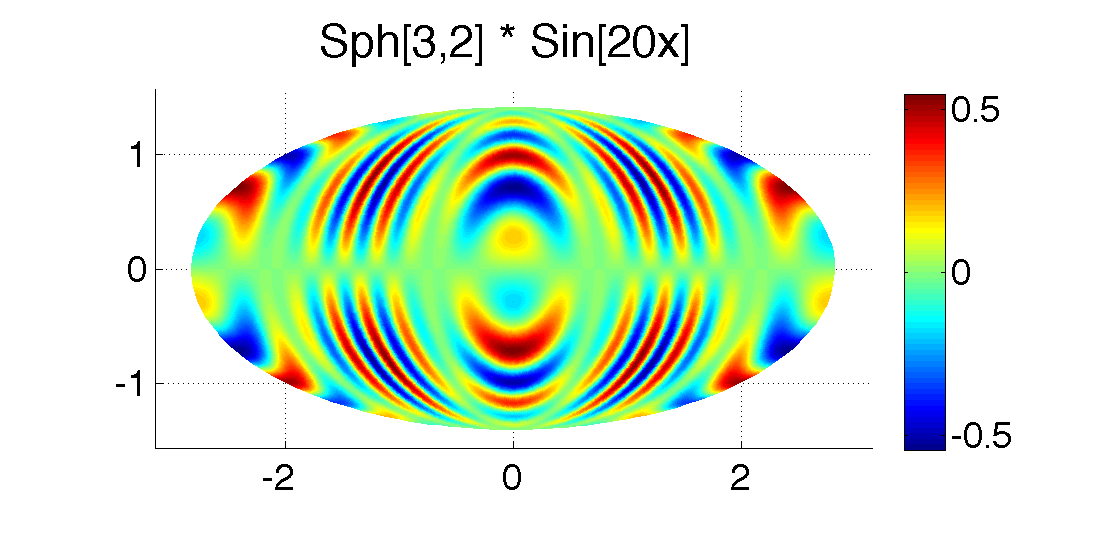
\includegraphics[width=1.0\textwidth]{../figures/appendices/direct_vs_indirect_weights/compare_weight_generation/xsfc_vs_xsfc_alt_on_sph32_times_sine_20x/sph32_times_sin20x.eps}
	\caption{Test function:  \\ $Y_{3}^{2} \sin(20 x) $.  }
	\end{subfigure}
	
	\begin{subfigure}[t]{0.48\textwidth}
		\centering
	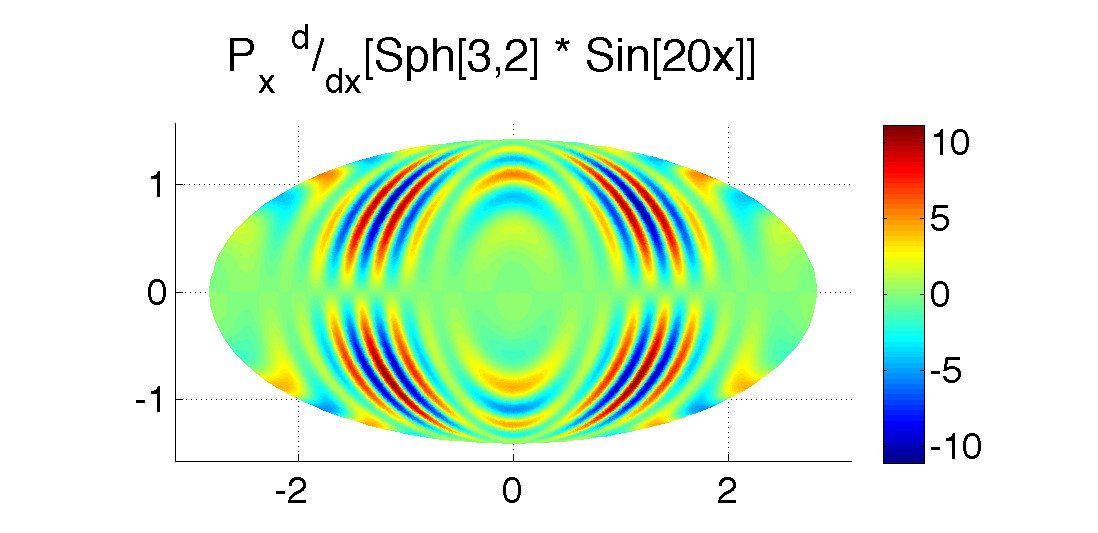
\includegraphics[width=1.0\textwidth]{../figures/appendices/direct_vs_indirect_weights/compare_weight_generation/xsfc_vs_xsfc_alt_on_sph32_times_sine_20x/pdx_sph32_times_sin20x.eps}
	\caption{$\mathbf{p}_{x} \cdot \nabla ( Y_{3}^{2} \sin(20 x))$ }
	\end{subfigure}
	\begin{subfigure}[t]{0.48\textwidth}
		\centering
	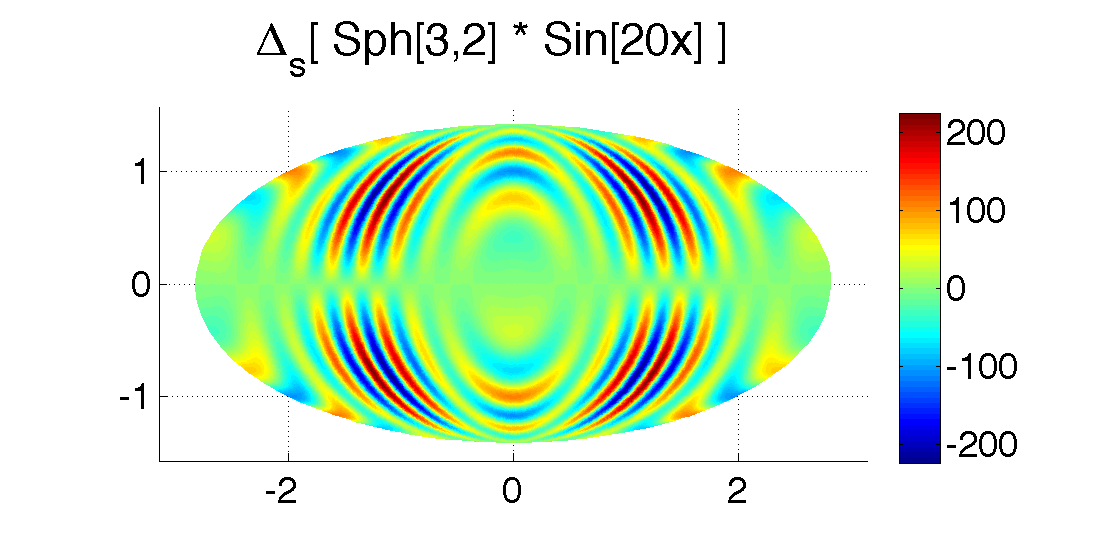
\includegraphics[width=1.0\textwidth]{../figures/appendices/direct_vs_indirect_weights/compare_weight_generation/lsfc_vs_px_grad_dot_px_grad/lsfc_sph32_times_sin20x.eps}
	\caption{Surface Laplacian: \\ $\LaplaceBeltrami ( Y_{3}^{2} \sin(20 x) )$  }
	\end{subfigure}
	\caption{Test function and its projected derivatives on the surface of the unit sphere. }
	\end{center}
\end{figure}

\begin{figure}
	\centering
	\begin{subfigure}[t]{0.48\textwidth}
	\includegraphics[width=1.0\textwidth]{../figures/appendices/direct_vs_indirect_weights/compare_weight_generation/xsfc_vs_xsfc_alt_on_sph32_times_sine_20x/direct_rel_l2_error.eps}
	\caption{$\mathbf{p}_{x} \cdot \nabla ( Y_{3}^{2} \sin(20 x))$ }
	\end{subfigure}
	\begin{subfigure}[t]{0.48\textwidth}
	\includegraphics[width=1.0\textwidth]{../figures/appendices/direct_vs_indirect_weights/compare_weight_generation/lsfc_vs_px_grad_dot_px_grad/direct_rel_l2_error.eps}
	\caption{$\LaplaceBeltrami ( Y_{3}^{2} \sin(20 x) )$}
    \end{subfigure}
	\caption{Relative $\ell_{2}$ error in differentiation.}
\end{figure}


\begin{figure}
	\centering
	\begin{subfigure}[t]{0.48\textwidth}
	\includegraphics[width=1.0\textwidth]{../figures/appendices/direct_vs_indirect_weights/compare_weight_generation/xsfc_vs_xsfc_alt_on_sph32_times_sine_20x/diff_of_rel_l2_errors.eps}
	\caption{$\mathbf{p}_{x} \cdot \nabla ( Y_{3}^{2} \sin(20 x))$}
	\end{subfigure}
		\begin{subfigure}[t]{0.48\textwidth}
	\centering
	\includegraphics[width=1.0\textwidth]{../figures/appendices/direct_vs_indirect_weights/compare_weight_generation/lsfc_vs_px_grad_dot_px_grad/diff_of_rel_l2_errors.eps}
	\caption{$\LaplaceBeltrami ( Y_{3}^{2} \sin(20 x) )$ (Indirect error is significantly higher for small resolutions. This likely due to compounding errors from the operator $P_x (D_x D_x + D_y D_y + D_z D_z)$). Where negative this figure indicates that the error is higher for indirect weight calculation. }
	\end{subfigure}
	\caption{Signed differences of relative $\ell_{2}$ errors in differentiation between Direct and Indirect weights. The sign indicates on the error indicates the higher of the two weight approaches.}
\end{figure}


\begin{figure}
	\centering
		\begin{subfigure}[t]{0.48\textwidth}
		\centering
	\includegraphics[width=1.0\textwidth]{../figures/appendices/direct_vs_indirect_weights/compare_weight_generation/xsfc_vs_xsfc_alt_on_sph32_times_sine_20x/abs_diff_of_rel_l2_errors.eps}
	\caption{$\mathbf{p}_{x} \cdot \nabla ( Y_{3}^{2} \sin(20 x))$}
	\end{subfigure}
	\begin{subfigure}[t]{0.48\textwidth}
	\centering
	\includegraphics[width=1.0\textwidth]{../figures/appendices/direct_vs_indirect_weights/compare_weight_generation/lsfc_vs_px_grad_dot_px_grad/abs_diff_of_rel_l2_errors.eps}
	\caption{$\LaplaceBeltrami ( Y_{3}^{2} \sin(20 x) )$}
	\end{subfigure}
		\caption{Absolute differences of relative $\ell_{2}$ errors in differentiation between Direct and Indirect weights.}
\end{figure}

%% NOT USEFUL: %%
%\begin{figure}[htbp]
%\centering
%\includegraphics[width=0.425\textwidth]{../figures/chapter2/compare_weight_generation/xsfc_vs_xsfc_alt_on_sph32/condest_dm_xsfc.pdf}
%\caption{Condition number estimates (condest) of direct $\mathbf{p}_{x}\nabla$ differentiation matrix}
%\end{figure}


\section{Conclusions}

%TODO: It appears that indirect weight calculations function. 
%TODO: They do have potential for savings
%TODO: Low resolution amplifies the errors in indirect weights. 
%TODO: still need to compare with the RBF-GA stable weight methods. What if stable weights initially resolve the extra error we see for small resolutions?




%Although it is clear the indirect method functions well compared to the direct method, we must consider its usefulness. Typically, weights are computed only as necessary for a PDE. If the PDE is on the sphere, then directly computing the $\mathbf{P}\cdot \nabla$ operator would be most efficient for both memory and computation. However, one could imagine a scenario such as a 3-D spherical shell domain with physics on the boundaries that must be constrained to the surface, while the interior requires only an unprojected $\nabla$ operator. In such cases, by simply computing for the $\nabla$ operator, we assemble all necessary operators with minimal loss of accuracy and significant savings ($3Nn$ doubles) in storage. 


%\ifstandalone
%\bibliographystyle{plain}
%\bibliography{merged_references}
%\end{document}
%\else
%\expandafter\endinput
%\fi


\ifstandalone
\bibliographystyle{plain}
\bibliography{merged_references}
\end{document}
\else
\expandafter\endinput
\fi

